  %%% -*-LaTeX-*-
%%% ====================================================================
%%% This is a sample top-level LaTeX-2e file for typesetting a thesis
%%% or dissertation at the University of Utah.  Most students find it
%%% convenient to start with a COPY of this file as a template, and
%%% then alter that copy to match their needs.
%%%
%%% There is an associated Unix Makefile that can be similarly
%%% customized, and then the only command ever needed to typeset the
%%% complete thesis is the single word "make".  Of course, during
%%% writing and typesetting, not all of the steps are needed, so
%%% often, one can just name a convenience target such as "make
%%% dvi-pass" or "make pdf-pass" to do just a single pass of LaTeX and
%%% BibTeX.
%%%
%%% There should be no, or very few, macro definitions in this file;
%%% any needed belong in a private style file, called mythesis.sty,
%%% and input below after all other packages.  The bulk of this file
%%% should just be command invocations, and any arguments that they
%%% need.
%%%
%%% We exploit the fact that TeX ignores spaces after command names to
%%% line up arguments for better readability.
%%%
%%% Each chapter should be a separate complete file, so that you can
%%% insert a command like \includeonly{chap_intro} before the first
%%% \include{chap_xxx} command to avoid typesetting all but the
%%% chapter that you are currently working on, to save time.
%%%
%%% Remember that occupants of job positions change jobs from time to
%%% time: YOU are responsible for ensuring correct names of all humans
%%% mentioned in this file!
%%%
%%% [16-Mar-2016]
%%% ====================================================================

\documentclass[11pt,Chicago]{uuthesis2e}

%%% Undefine two macros from uuthesis2e.cls that conflict with
%%% definitions in amsthm.sty that fail to check for prior definitions!
%%% NB: The amsthm package refines the LaTeX theorem environment,
%%% and the uuthesis-color-headings wraps that definition, so the
%%% amsthm package must be read first!
\let \proof    = \relax
\let \endproof = \relax
\usepackage {amsthm}

%%% ====================================================================
%%% Choose an alternate font family for the document if the TeX default
%%% of Computer Modern is not wanted:

\usepackage{mathpazo}

%%% ====================================================================
%%% Some miscellaneous Utah- and student-specific settings:
%%%
%%% Chapter is one level, section and subsection are the next two levels.

\fourlevels

%%% ====================================================================
%%% The remaining packages are required by this particular thesis,
%%% but other theses will almost certainly need different packages:
%%%
%%% WARNING: MANY \LaTeX{} packages change dimensions, glue, and/or
%%% formatting styles, and such changes are likely to conflict with
%%% University of Utah Thesis Office requirements.  Therefore, minimize
%%% the number of packages that you include!

\usepackage {amsmath}
\usepackage {amssymb}
\usepackage {bm}
\usepackage {bibnames}
\usepackage {citesort}
\usepackage {graphicx}
\usepackage {graphpap}
\usepackage {longtable}
\usepackage {multirow}
\usepackage {tikz}
\usetikzlibrary {decorations.markings}
\usepackage {varioref}

%%% ====================================================================
%%% Support for a subject index:

\usepackage {uuthesis-index}

%%% ====================================================================
%%% The various uuthesis-*.sty packages must come AFTER all other
%%% system-provided packages, so that they can correctly override
%%% settings from those packages.

%%% Include latest updates for 2016 (WARNING: the name is subject to
%%% change: see http://www.math.utah.edu/pub/uuthesis/ for the most
%%% current version.)

\usepackage {uuthesis-2016-h}  % MANDATORY package

%%% This is an OPTIONAL package that sets chapter and sectional headings
%%% in color:
%%% Use one or the other of these:
% \usepackage {color}
\usepackage {uuthesis-color-headings}
\definecolor{utahheadingcolor} {rgb}  {0.7, 0.0, 0.0}
\definecolor{utahtheoremcolor} {rgb}  {0.490,0.149,0.804} % purple4
\definecolor{utahtheoremcolor} {rgb}  {0.545,0.137,0.137} % brown4

%%% Here is another, and more convenient, way to define colors, via
%%% aliases of named colors in the X11-derived rgb.sty file

\usepackage{coloralias}
\definecoloralias{utahheadingcolor}{steelblue4}
\definecoloralias{utahtheoremcolor}{hotpink3}
\usepackage{textcomp}
\usepackage{url}
\usepackage{booktabs}
\usepackage{listings}
\usepackage{csquotes}
\usepackage{float}
%\usepackage{caption}
\usepackage{xr}
\usepackage{subcaption}
\captionsetup{compatibility=false}




%%% The default heading color is utahred (defined by University Printing
%%% Services as 0.8 red, 0.0 green, 0.0 blue), but you could redefine
%%% that to, for example, a dark blue color, like this AFTER including
%%% the package:
%%%
%%%     \definecolor{utahheading}{rgb}{0,0,0.8}
%%%
%%% NB: Be careful with use of colors in typesetting, and in figures,
%%% because about 6 percent of the human male population is red/green
%%% color blind: they see those colors as shades of brown.  Red and
%%% blue, or blue and green, are better choices for choosing
%%% distinguishable colors.  Also, avoid light colors, especially
%%% yellow, because they are hard to see against white paper and
%%% screen backgrounds, and when printed on black-and-white printers,
%%% where they are rendered in gray, they may be too faint to read.

%%% ====================================================================
%%% Support for a subject index:

\usepackage {uuthesis-index}

%%% ====================================================================
%%% This single user-specific file is where all personal customizations
%%% and macro definitions should be placed, and it should come LAST,
%%% after ALL OTHER packages, in case it needs to override some of their
%%% definitions.

\usepackage {mythesis}

%%% ====================================================================
%%% The student-specific front matter fields are defined here:

\author                 {Aniraj Kesavan}
\title                  {Making Large Transfers Fast \\For In-Memory Databases\\ In Modern Networks}
\thesistype             {thesis}

\dedication             {To my parents and teachers, Kindergarten to the U}

%%% Most students need just a short degree name, like this:
\degree                 {M.S}
%%% However, multiline degrees are possible, and are done like this:
\degree                 {Master of Science \\
                         in \\
                         Computer Science}

%%% College- and Department-level definitions:
\approvaldepartment     {Computing}
\department             {School of Computing}
\graduatedean           {David B Kieda}
\departmentchair        {Ross Whitaker}

%%% The graduate student's committee members:
\committeechair         {Ryan Stutsman}
\firstreader            {Robert Ricci}
\secondreader           {Feifei Li}
\chairtitle             {Assistant Professor}

%%% NB: It is rare, but possible, for there to be two chairs, For
%%% example, one student had
%%%
%%% \committeechair{\mbox{\small Andrej Cherkaev and Andrejs Treibergs}}
%%%
%%% The \mbox{} ensures that line breaks cannot happen, and the \small
%%% is necessary to make the names fit on the Dissertation Approval form

%%% Dates that must be adjusted for each academic term, and be permitted
%%% according to the University of Utah Thesis Office:
\submitdate             {May  2017}
\copyrightyear          {2017}

%%% Dates on which committee members approved the thesis
\chairdateapproved      {23 Feb 2017}
\firstdateapproved      {23 Feb 2017}
\seconddateapproved     {23 Feb 2017}
\thirddateapproved      {23 Feb 2017}
\fourthdateapproved     {23 Feb 2017}

%%% ====================================================================
%%% Typesetting begins here:

\begin{document}

%% Comment out items by inserting a percent % character
\frontmatterformat
\titlepage
\copyrightpage
\dissertationapproval
\setcounter {page}     {2}             % UofU Thesis Office demands abstract on p. iii: start one lower
\preface    {abstract} {Abstract}
%\preface {timeline-preface} {Timeline}
\dedicationpage
\tableofcontents
\listoffigures
%\listoftables
%
%%% Optional front matter page(s), made from source "notation.tex". If
%%% you don't need it, then comment out the \optionalfront command
%%% line!  The first argument is the (unnumbered) section header for
%%% the text supplied by the file input by the second argument; that
%%% file must NOT contain \chapter, \section, \subsection, \ldots{}
%%% sectioning commands.

%\optionalfront {Notation and Symbols} {%%% -*-LaTeX-*-
%%%
%%% This is notation.tex.
%%%
%%% This file is included in a thesis with a front-matter command
%%%
%%%     \optionalfront {Notation and Symbols} {%%% -*-LaTeX-*-
%%%
%%% This is notation.tex.
%%%
%%% This file is included in a thesis with a front-matter command
%%%
%%%     \optionalfront {Notation and Symbols} {%%% -*-LaTeX-*-
%%%
%%% This is notation.tex.
%%%
%%% This file is included in a thesis with a front-matter command
%%%
%%%     \optionalfront {Notation and Symbols} {\input{notation}}
%%%
%%% The heading for this material is provided by the first argument
%%% so none needs to be supplied here.

\begin{tabular}{ll}
    \hline
    $\alpha$      & fine-structure (dimensionless) constant, approximately $1 / 137$ \\
    $\alpha$      & radiation of doubly-ionized helium ions, He++ \\
    $\beta$       & radiation of electrons \\
    $\gamma$      & radiation of very high frequency, beyond that of X rays \\
    $\gamma$      & Euler's constant, approximately $0.577\,215\,\ldots{}$  \\
    $\delta$      & stepsize in numerical integration \\
    $\delta(x)$   & Dirac's famous function \\
    $\epsilon$    & a tiny number, usually in the context of a limit to zero \\
    $\zeta(x)$    & the famous Riemann zeta function \\
    \ldots{}      & \ldots{}  \\
    $\psi(x)$     & logarithmic derivative of the gamma function \\
    $\omega$      & frequency \\
    \hline
\end{tabular}
}
%%%
%%% The heading for this material is provided by the first argument
%%% so none needs to be supplied here.

\begin{tabular}{ll}
    \hline
    $\alpha$      & fine-structure (dimensionless) constant, approximately $1 / 137$ \\
    $\alpha$      & radiation of doubly-ionized helium ions, He++ \\
    $\beta$       & radiation of electrons \\
    $\gamma$      & radiation of very high frequency, beyond that of X rays \\
    $\gamma$      & Euler's constant, approximately $0.577\,215\,\ldots{}$  \\
    $\delta$      & stepsize in numerical integration \\
    $\delta(x)$   & Dirac's famous function \\
    $\epsilon$    & a tiny number, usually in the context of a limit to zero \\
    $\zeta(x)$    & the famous Riemann zeta function \\
    \ldots{}      & \ldots{}  \\
    $\psi(x)$     & logarithmic derivative of the gamma function \\
    $\omega$      & frequency \\
    \hline
\end{tabular}
}
%%%
%%% The heading for this material is provided by the first argument
%%% so none needs to be supplied here.

\begin{tabular}{ll}
    \hline
    $\alpha$      & fine-structure (dimensionless) constant, approximately $1 / 137$ \\
    $\alpha$      & radiation of doubly-ionized helium ions, He++ \\
    $\beta$       & radiation of electrons \\
    $\gamma$      & radiation of very high frequency, beyond that of X rays \\
    $\gamma$      & Euler's constant, approximately $0.577\,215\,\ldots{}$  \\
    $\delta$      & stepsize in numerical integration \\
    $\delta(x)$   & Dirac's famous function \\
    $\epsilon$    & a tiny number, usually in the context of a limit to zero \\
    $\zeta(x)$    & the famous Riemann zeta function \\
    \ldots{}      & \ldots{}  \\
    $\psi(x)$     & logarithmic derivative of the gamma function \\
    $\omega$      & frequency \\
    \hline
\end{tabular}
}

%%% Uncomment this is you want the contents of acknowledge.tex typeset here.
%%% Note that both "Acknowledgement" and "Acknowledgment" are accepted
%%% spellings of that word.

\preface{acknowledge}{Acknowledgements}

%%% Demonstrations of thesis typesetting features for the sample thesis.
%%% Once you have seen the examples, you can comment out this line.
%\optionalfront {Typesetting Experiments} {%%% -*-LaTeX-*-
%%% ====================================================================
%%% This file is intended to be included as a front-matter section of
%%% the sample thesis, with a command like this
%%%
%%% \optionalfront{Typesetting Experiments}{%%% -*-LaTeX-*-
%%% ====================================================================
%%% This file is intended to be included as a front-matter section of
%%% the sample thesis, with a command like this
%%%
%%% \optionalfront{Typesetting Experiments}{%%% -*-LaTeX-*-
%%% ====================================================================
%%% This file is intended to be included as a front-matter section of
%%% the sample thesis, with a command like this
%%%
%%% \optionalfront{Typesetting Experiments}{\input{samples}}
%%%
%%% just before the \maintext macro that begins the body of the thesis,
%%% and starts chapter numbering.
%%%
%%% [16-Mar-2016]
%%% ====================================================================

\input{rgb.sty}

\definecolor{utahred} {rgb} {0.8, 0.0, 0.0} % official definition for University of Utah Printing Services

\doublespace

%% \showthe \baselineskip

In this section, we use color in several places.
The \verb=\colorbox= command takes two arguments
--- a named color and text to be in black on a
background of that color --- and sets the text in
a box with a small margin of width \verb=\fboxsep=
(set to \texttt{\the\fboxsep} in this document).

Here, we want a tighter colored box that has a
fixed height, and is independent of letter shape.
We set the margin to zero inside a group so that
the change is purely local, and so that height and
depth of the line are not increased over what they
would be if the colored box were not used.  We
prefix a \TeX{} \verb=\strut= to the user-supplied
text, because that command expands to a zero-width
box of the height and depth of parentheses, which,
in most fonts, delimit the extent of letter
shapes.

\begin{verbatim}
\newcommand {\hilitebox} [1] {{\fboxsep = 0pt\colorbox{pink}{\strut #1}}}
\end{verbatim}

\newcommand {\hilitebox} [1] {{\fboxsep = 0pt\colorbox{pink}{\strut #1}}}

Here is a fragment from the first chapter in another
thesis, set in \emph{emphasized text} to distinguish it
from the rest of this section:

\begin{itshape}
    In light of the known results, the consistency
    of empirical semivariogram and related
    estimators is widely considered a settled
    matter.  For example, Lahiri, Lee, and Cressie
    \cite{Lahiri:2002:ADA} state:

    \begin{quote}
        The simpler and more commonly used
        nonparametric estimators of the variogram,
        such as the method of moments estimator of
        Matheron (1962) and its robustified
        versions due to Cressie and Hawkins (1980)
        have many desirable properties like,
        unbiasedness, consistency, etc. \ldots
    \end{quote}
    \noindent
    Regarding a kernel estimator of the covariance
    function, Hall and Patil
    \cite{Hall:1994:PNE} remarked:
    \begin{quote}
        It is not difficult to see that if, as $ n
        $ increases, the points $ t_i $ become
        increasingly dense in each bounded subset
        of $ \mathbb{R}^d $, then the bandwidth $
        h $ may be chosen so that $ \check \rho(t)
        \to \rho(t) $ as $ n \to \infty $, for
        each $ t \in \mathbb{R}^d $.
    \end{quote}
    However, in order to be true, such statements
    would need to be qualified by many assumptions
    on the random field as well as on the
    observation locations. We will see in
    \S2.3 that even for well-behaved
    random fields (e.g., $\rho^*$-mixing Gaussian
    random fields), it is not enough to assume
    that the observation locations become
    increasingly dense in each bounded subset; a
    stronger assumption must be made to ensure
    that the observation locations do not become
    denser in one region too much faster than in
    others.
\end{itshape}

The text before the previous paragraph contained
two \texttt{quote} environments separated by a
line of prose.  Here are some more tests of both
kinds of \LaTeX{} environments for showing text
written by someone else.

This is a \hilitebox{\texttt{quote}} environment
with one short line, following a fairly short
paragraph of prose (in this, and following
examples, the text is explicitly colored with a
command like \verb=\color{purple}= inside the
environment before the text):
%
\begin{singlespace}
\color{darkblue}
\begin{verbatim}
\begin{quote}
    \color{purple}
    14 March 2016 is $\pi \approx 3.1416$ day in funny notation.
    \hfill \emph{Web news reports}
\end{quote}
\end{verbatim}
\end{singlespace}
%
\begin{quote}
    \color{purple}
    14 March 2016 is $\pi \approx 3.1416$ day in funny notation.
    \hfill \emph{Web news reports}
\end{quote}

This is a \hilitebox{\texttt{quote}} environment
with three short lines, each a separate paragraph,
following a fairly short paragraph of prose.

\begin{singlespace}
\color{darkblue}
\begin{verbatim}
\begin{quote}
    \color{forestgreen}
    14 March 2016 is $\pi \approx 3.1416$ day in funny notation.
    \hfill \emph{Web news reports}

    14 March 2016 is $\pi \approx 3.1416$ day in funny notation.
    \hfill \emph{Web news reports}

    14 March 2016 is $\pi \approx 3.1416$ day in funny notation.
    \hfill \emph{Web news reports}
\end{quote}
\end{verbatim}
\end{singlespace}
%
\begin{quote}
    \color{forestgreen}
    14 March 2016 is $\pi \approx 3.1416$ day in funny notation.
    \hfill \emph{Web news reports}

    14 March 2016 is $\pi \approx 3.1416$ day in funny notation.
    \hfill \emph{Web news reports}

    14 March 2016 is $\pi \approx 3.1416$ day in funny notation.
    \hfill \emph{Web news reports}
\end{quote}

Here is another example, this time with separate
colors for each paragraph:

\begin{singlespace}
\color{darkblue}
\begin{verbatim}
\begin{quote}
    \color{darkkhaki}
    14 March 2016 is $\pi \approx 3.1416$ day in funny notation.
    \hfill \emph{Web news reports}

    \color{darkmagenta}
    14 March 2016 is $\pi \approx 3.1416$ day in funny notation.
    \hfill \emph{Web news reports}

    \color{darkcyan}
    14 March 2016 is $\pi \approx 3.1416$ day in funny notation.
    \hfill \emph{Web news reports}

    \color{darkorange}
    14 March 2016 is $\pi \approx 3.1416$ day in funny notation.
    14 March 2016 is $\pi \approx 3.1416$ day in funny notation.
    14 March 2016 is $\pi \approx 3.1416$ day in funny notation.
    \linebreak
    \strut
    \hfill \emph{Web news reports}
\end{quote}
\end{verbatim}
\end{singlespace}
%
\begin{quote}
    \color{darkkhaki}
    14 March 2016 is $\pi \approx 3.1416$ day in funny notation.
    \hfill \emph{Web news reports}

    \color{darkmagenta}
    14 March 2016 is $\pi \approx 3.1416$ day in funny notation.
    \hfill \emph{Web news reports}

    \color{darkcyan}
    14 March 2016 is $\pi \approx 3.1416$ day in funny notation.
    \hfill \emph{Web news reports}

    \color{darkorange}
    14 March 2016 is $\pi \approx 3.1416$ day in funny notation.
    14 March 2016 is $\pi \approx 3.1416$ day in funny notation.
    14 March 2016 is $\pi \approx 3.1416$ day in funny notation.
    \linebreak
    \strut
    \hfill \emph{Web news reports}
\end{quote}

Notice that \hilitebox{\texttt{quote}} paragraphs
are \emph{not} indented, but the environment
itself \emph{is} indented on the left and right by
the value of \verb=\leftmargin= (set to
\texttt{\the\leftmargin} in this document, which
should be identical to \verb=2.5em=, where
\verb=1em= = \texttt{\dimen0 = 1em \the\dimen0}).

For debugging purposes, we also have
\verb=\leftmargini= set to
\texttt{\the\leftmargini}, and we have
\verb=\leftmarginii= set to
\texttt{\the\leftmarginii}.

This is a \hilitebox{\texttt{quotation}}
environment with one paragraph, following a fairly
short paragraph of prose (notice that the
\texttt{quotation} paragraphs \emph{are}
indented):

\begin{singlespace}
\color{darkblue}
\begin{verbatim}
\begin{quotation}
    \color{blue}
    Algebra is concerned with manipulation in
    \emph{time}, and geometry is concerned with
    \emph{space}. These are two orthogonal aspects
    of the world, and they represent two different
    points of view in mathematics.  Thus the
    argument or dialogue between mathematicians in
    the past about the relative importance of
    geometry and algebra represents something very
    fundamental.
    \hfill
    \emph{Sir Michael Atiyah}
    % Mathematics in the 20$^{th}$ century
    % NTM {\bf 10}(1--3) 25--39 (September 2002)
    % http://dx.doi.org/10.1007/BF03033096
\end{quotation}
\end{verbatim}
\end{singlespace}
%
\begin{quotation}
    \color{blue}
    Algebra is concerned with manipulation in
    \emph{time}, and geometry is concerned with
    \emph{space}. These are two orthogonal aspects
    of the world, and they represent two different
    points of view in mathematics.  Thus the
    argument or dialogue between mathematicians in
    the past about the relative importance of
    geometry and algebra represents something very
    fundamental.
    \hfill
    \emph{Sir Michael Atiyah}
    % Mathematics in the 20$^{th}$ century
    % NTM {\bf 10}(1--3) 25--39 (September 2002)
    % http://dx.doi.org/10.1007/BF03033096
\end{quotation}

This is a \hilitebox{\texttt{quotation}} environment with three
paragraphs, following a fairly short paragraph of prose:

\begin{quotation}
    \color{utahred}
    Algebra is concerned with manipulation in
    \emph{time}, and geometry is concerned with
    \emph{space}. These are two orthogonal aspects
    of the world, and they represent two different
    points of view in mathematics.  Thus the
    argument or dialogue between mathematicians in
    the past about the relative importance of
    geometry and algebra represents something very
    fundamental.
    \hfill
    \emph{Sir Michael Atiyah}

    Algebra is concerned with manipulation in
    \emph{time}, and geometry is concerned with
    \emph{space}. These are two orthogonal aspects
    of the world, and they represent two different
    points of view in mathematics.  Thus the
    argument or dialogue between mathematicians in
    the past about the relative importance of
    geometry and algebra represents something very
    fundamental.
    \hfill
    \emph{Sir Michael Atiyah}

    Algebra is concerned with manipulation in
    \emph{time}, and geometry is concerned with
    \emph{space}. These are two orthogonal aspects
    of the world, and they represent two different
    points of view in mathematics.  Thus the
    argument or dialogue between mathematicians in
    the past about the relative importance of
    geometry and algebra represents something very
    fundamental.
    \hfill
    \emph{Sir Michael Atiyah}
\end{quotation}

%% \showthe \baselineskip

Now all following text should be back in
double-spaced mode, and just go on and on and on
and on and on and on and on and on and on and on
and on and on and on and on and on and on and on
and on and on and on and on and on and on and on
and on and on and on and on and on and on and on
and on and on and on and on and on and on and on
and on and on and on and on and on and on and on
and on and on and on and on and on and on and on
and on and on and on and on and on and on and on
and on and on and on and on and on and on and on
and on and on and on and on and on and on and on
and on and on and on and on \ldots{}.

%% \showthe \baselineskip

Now all following text should be back in
double-spaced mode, and just go on and on and on
and on and on and on and on and on and on and on
and on and on and on and on and on and on and on
and on and on and on and on and on and on and on
and on and on and on and on and on and on and on
and on and on and on and on and on and on and on
and on and on and on and on and on and on and on
and on and on and on and on and on and on and on
and on and on and on and on and on and on and on
and on and on and on and on and on and on and on
and on and on and on and on and on and on and on
and on and on and on and on \ldots{}.

%%% \showthe \baselineskip
}
%%%
%%% just before the \maintext macro that begins the body of the thesis,
%%% and starts chapter numbering.
%%%
%%% [16-Mar-2016]
%%% ====================================================================

%% Derived from file://ibapah.math.utah.edu/usr/lib/X11/rgb.txt
%% on Wed Jun  9 11:48:18 MDT 2004
%% by ~beebe/src/awk/rgb.awk

\definecolor{aliceblue}{rgb}{0.941,0.973,1}                    	% #f0f8ff 240 248 255 AliceBlue
\definecolor{antiquewhite1}{rgb}{1,0.937,0.859}                	% #ffefdb 255 239 219 AntiqueWhite1
\definecolor{antiquewhite2}{rgb}{0.933,0.875,0.800}            	% #eedfcc 238 223 204 AntiqueWhite2
\definecolor{antiquewhite3}{rgb}{0.804,0.753,0.690}            	% #cdc0b0 205 192 176 AntiqueWhite3
\definecolor{antiquewhite4}{rgb}{0.545,0.514,0.471}            	% #8b8378 139 131 120 AntiqueWhite4
\definecolor{antiquewhite}{rgb}{0.980,0.922,0.843}             	% #faebd7 250 235 215 AntiqueWhite
\definecolor{aquamarine1}{rgb}{0.498,1,0.831}                  	% #7fffd4 127 255 212 aquamarine1
\definecolor{aquamarine2}{rgb}{0.463,0.933,0.776}              	% #76eec6 118 238 198 aquamarine2
\definecolor{aquamarine3}{rgb}{0.400,0.804,0.667}              	% #66cdaa 102 205 170 aquamarine3
\definecolor{aquamarine4}{rgb}{0.271,0.545,0.455}              	% #458b74 69 139 116 aquamarine4
\definecolor{aquamarine}{rgb}{0.498,1,0.831}                   	% #7fffd4 127 255 212 aquamarine
\definecolor{azure1}{rgb}{0.941,1,1}                           	% #f0ffff 240 255 255 azure1
\definecolor{azure2}{rgb}{0.878,0.933,0.933}                   	% #e0eeee 224 238 238 azure2
\definecolor{azure3}{rgb}{0.757,0.804,0.804}                   	% #c1cdcd 193 205 205 azure3
\definecolor{azure4}{rgb}{0.514,0.545,0.545}                   	% #838b8b 131 139 139 azure4
\definecolor{azure}{rgb}{0.941,1,1}                            	% #f0ffff 240 255 255 azure
\definecolor{beige}{rgb}{0.961,0.961,0.863}                    	% #f5f5dc 245 245 220 beige
\definecolor{bisque1}{rgb}{1,0.894,0.769}                      	% #ffe4c4 255 228 196 bisque1
\definecolor{bisque2}{rgb}{0.933,0.835,0.718}                  	% #eed5b7 238 213 183 bisque2
\definecolor{bisque3}{rgb}{0.804,0.718,0.620}                  	% #cdb79e 205 183 158 bisque3
\definecolor{bisque4}{rgb}{0.545,0.490,0.420}                  	% #8b7d6b 139 125 107 bisque4
\definecolor{bisque}{rgb}{1,0.894,0.769}                       	% #ffe4c4 255 228 196 bisque
\definecolor{black}{rgb}{0,0,0}                                	% #000000 0 0 0 black
\definecolor{blanchedalmond}{rgb}{1,0.922,0.804}               	% #ffebcd 255 235 205 BlanchedAlmond
\definecolor{blue1}{rgb}{0,0,1}                                	% #0000ff 0 0 255 blue1
\definecolor{blue2}{rgb}{0,0,0.933}                            	% #0000ee 0 0 238 blue2
\definecolor{blue3}{rgb}{0,0,0.804}                            	% #0000cd 0 0 205 blue3
\definecolor{blue4}{rgb}{0,0,0.545}                            	% #00008b 0 0 139 blue4
\definecolor{blue}{rgb}{0,0,1}                                 	% #0000ff 0 0 255 blue
\definecolor{blueviolet}{rgb}{0.541,0.169,0.886}               	% #8a2be2 138 43 226 BlueViolet
\definecolor{brown1}{rgb}{1,0.251,0.251}                       	% #ff4040 255 64 64 brown1
\definecolor{brown2}{rgb}{0.933,0.231,0.231}                   	% #ee3b3b 238 59 59 brown2
\definecolor{brown3}{rgb}{0.804,0.200,0.200}                   	% #cd3333 205 51 51 brown3
\definecolor{brown4}{rgb}{0.545,0.137,0.137}                   	% #8b2323 139 35 35 brown4
\definecolor{brown}{rgb}{0.647,0.165,0.165}                    	% #a52a2a 165 42 42 brown
\definecolor{burlywood1}{rgb}{1,0.827,0.608}                   	% #ffd39b 255 211 155 burlywood1
\definecolor{burlywood2}{rgb}{0.933,0.773,0.569}               	% #eec591 238 197 145 burlywood2
\definecolor{burlywood3}{rgb}{0.804,0.667,0.490}               	% #cdaa7d 205 170 125 burlywood3
\definecolor{burlywood4}{rgb}{0.545,0.451,0.333}               	% #8b7355 139 115 85 burlywood4
\definecolor{burlywood}{rgb}{0.871,0.722,0.529}                	% #deb887 222 184 135 burlywood
\definecolor{cadetblue1}{rgb}{0.596,0.961,1}                   	% #98f5ff 152 245 255 CadetBlue1
\definecolor{cadetblue2}{rgb}{0.557,0.898,0.933}               	% #8ee5ee 142 229 238 CadetBlue2
\definecolor{cadetblue3}{rgb}{0.478,0.773,0.804}               	% #7ac5cd 122 197 205 CadetBlue3
\definecolor{cadetblue4}{rgb}{0.325,0.525,0.545}               	% #53868b 83 134 139 CadetBlue4
\definecolor{cadetblue}{rgb}{0.373,0.620,0.627}                	% #5f9ea0 95 158 160 CadetBlue
\definecolor{chartreuse1}{rgb}{0.498,1,0}                      	% #7fff00 127 255 0 chartreuse1
\definecolor{chartreuse2}{rgb}{0.463,0.933,0}                  	% #76ee00 118 238 0 chartreuse2
\definecolor{chartreuse3}{rgb}{0.400,0.804,0}                  	% #66cd00 102 205 0 chartreuse3
\definecolor{chartreuse4}{rgb}{0.271,0.545,0}                  	% #458b00 69 139 0 chartreuse4
\definecolor{chartreuse}{rgb}{0.498,1,0}                       	% #7fff00 127 255 0 chartreuse
\definecolor{chocolate1}{rgb}{1,0.498,0.141}                   	% #ff7f24 255 127 36 chocolate1
\definecolor{chocolate2}{rgb}{0.933,0.463,0.129}               	% #ee7621 238 118 33 chocolate2
\definecolor{chocolate3}{rgb}{0.804,0.400,0.114}               	% #cd661d 205 102 29 chocolate3
\definecolor{chocolate4}{rgb}{0.545,0.271,0.075}               	% #8b4513 139 69 19 chocolate4
\definecolor{chocolate}{rgb}{0.824,0.412,0.118}                	% #d2691e 210 105 30 chocolate
\definecolor{coral1}{rgb}{1,0.447,0.337}                       	% #ff7256 255 114 86 coral1
\definecolor{coral2}{rgb}{0.933,0.416,0.314}                   	% #ee6a50 238 106 80 coral2
\definecolor{coral3}{rgb}{0.804,0.357,0.271}                   	% #cd5b45 205 91 69 coral3
\definecolor{coral4}{rgb}{0.545,0.243,0.184}                   	% #8b3e2f 139 62 47 coral4
\definecolor{coral}{rgb}{1,0.498,0.314}                        	% #ff7f50 255 127 80 coral
\definecolor{cornflowerblue}{rgb}{0.392,0.584,0.929}           	% #6495ed 100 149 237 CornflowerBlue
\definecolor{cornsilk1}{rgb}{1,0.973,0.863}                    	% #fff8dc 255 248 220 cornsilk1
\definecolor{cornsilk2}{rgb}{0.933,0.910,0.804}                	% #eee8cd 238 232 205 cornsilk2
\definecolor{cornsilk3}{rgb}{0.804,0.784,0.694}                	% #cdc8b1 205 200 177 cornsilk3
\definecolor{cornsilk4}{rgb}{0.545,0.533,0.471}                	% #8b8878 139 136 120 cornsilk4
\definecolor{cornsilk}{rgb}{1,0.973,0.863}                     	% #fff8dc 255 248 220 cornsilk
\definecolor{cyan1}{rgb}{0,1,1}                                	% #00ffff 0 255 255 cyan1
\definecolor{cyan2}{rgb}{0,0.933,0.933}                        	% #00eeee 0 238 238 cyan2
\definecolor{cyan3}{rgb}{0,0.804,0.804}                        	% #00cdcd 0 205 205 cyan3
\definecolor{cyan4}{rgb}{0,0.545,0.545}                        	% #008b8b 0 139 139 cyan4
\definecolor{cyan}{rgb}{0,1,1}                                 	% #00ffff 0 255 255 cyan
\definecolor{darkblue}{rgb}{0,0,0.545}                         	% #00008b 0 0 139 DarkBlue
\definecolor{darkcyan}{rgb}{0,0.545,0.545}                     	% #008b8b 0 139 139 DarkCyan
\definecolor{darkgoldenrod1}{rgb}{1,0.725,0.059}               	% #ffb90f 255 185 15 DarkGoldenrod1
\definecolor{darkgoldenrod2}{rgb}{0.933,0.678,0.055}           	% #eead0e 238 173 14 DarkGoldenrod2
\definecolor{darkgoldenrod3}{rgb}{0.804,0.584,0.047}           	% #cd950c 205 149 12 DarkGoldenrod3
\definecolor{darkgoldenrod4}{rgb}{0.545,0.396,0.031}           	% #8b6508 139 101 8 DarkGoldenrod4
\definecolor{darkgoldenrod}{rgb}{0.722,0.525,0.043}            	% #b8860b 184 134 11 DarkGoldenrod
\definecolor{darkgray}{rgb}{0.663,0.663,0.663}                 	% #a9a9a9 169 169 169 DarkGray
\definecolor{darkgreen}{rgb}{0,0.392,0}                        	% #006400 0 100 0 DarkGreen
\definecolor{darkgrey}{rgb}{0.663,0.663,0.663}                 	% #a9a9a9 169 169 169 DarkGrey
\definecolor{darkkhaki}{rgb}{0.741,0.718,0.420}                	% #bdb76b 189 183 107 DarkKhaki
\definecolor{darkmagenta}{rgb}{0.545,0,0.545}                  	% #8b008b 139 0 139 DarkMagenta
\definecolor{darkolivegreen1}{rgb}{0.792,1,0.439}              	% #caff70 202 255 112 DarkOliveGreen1
\definecolor{darkolivegreen2}{rgb}{0.737,0.933,0.408}          	% #bcee68 188 238 104 DarkOliveGreen2
\definecolor{darkolivegreen3}{rgb}{0.635,0.804,0.353}          	% #a2cd5a 162 205 90 DarkOliveGreen3
\definecolor{darkolivegreen4}{rgb}{0.431,0.545,0.239}          	% #6e8b3d 110 139 61 DarkOliveGreen4
\definecolor{darkolivegreen}{rgb}{0.333,0.420,0.184}           	% #556b2f 85 107 47 DarkOliveGreen
\definecolor{darkorange1}{rgb}{1,0.498,0}                      	% #ff7f00 255 127 0 DarkOrange1
\definecolor{darkorange2}{rgb}{0.933,0.463,0}                  	% #ee7600 238 118 0 DarkOrange2
\definecolor{darkorange3}{rgb}{0.804,0.400,0}                  	% #cd6600 205 102 0 DarkOrange3
\definecolor{darkorange4}{rgb}{0.545,0.271,0}                  	% #8b4500 139 69 0 DarkOrange4
\definecolor{darkorange}{rgb}{1,0.549,0}                       	% #ff8c00 255 140 0 DarkOrange
\definecolor{darkorchid1}{rgb}{0.749,0.243,1}                  	% #bf3eff 191 62 255 DarkOrchid1
\definecolor{darkorchid2}{rgb}{0.698,0.227,0.933}              	% #b23aee 178 58 238 DarkOrchid2
\definecolor{darkorchid3}{rgb}{0.604,0.196,0.804}              	% #9a32cd 154 50 205 DarkOrchid3
\definecolor{darkorchid4}{rgb}{0.408,0.133,0.545}              	% #68228b 104 34 139 DarkOrchid4
\definecolor{darkorchid}{rgb}{0.600,0.196,0.800}               	% #9932cc 153 50 204 DarkOrchid
\definecolor{darkred}{rgb}{0.545,0,0}                          	% #8b0000 139 0 0 DarkRed
\definecolor{darksalmon}{rgb}{0.914,0.588,0.478}               	% #e9967a 233 150 122 DarkSalmon
\definecolor{darkseagreen1}{rgb}{0.757,1,0.757}                	% #c1ffc1 193 255 193 DarkSeaGreen1
\definecolor{darkseagreen2}{rgb}{0.706,0.933,0.706}            	% #b4eeb4 180 238 180 DarkSeaGreen2
\definecolor{darkseagreen3}{rgb}{0.608,0.804,0.608}            	% #9bcd9b 155 205 155 DarkSeaGreen3
\definecolor{darkseagreen4}{rgb}{0.412,0.545,0.412}            	% #698b69 105 139 105 DarkSeaGreen4
\definecolor{darkseagreen}{rgb}{0.561,0.737,0.561}             	% #8fbc8f 143 188 143 DarkSeaGreen
\definecolor{darkslateblue}{rgb}{0.282,0.239,0.545}            	% #483d8b 72 61 139 DarkSlateBlue
\definecolor{darkslategray1}{rgb}{0.592,1,1}                   	% #97ffff 151 255 255 DarkSlateGray1
\definecolor{darkslategray2}{rgb}{0.553,0.933,0.933}           	% #8deeee 141 238 238 DarkSlateGray2
\definecolor{darkslategray3}{rgb}{0.475,0.804,0.804}           	% #79cdcd 121 205 205 DarkSlateGray3
\definecolor{darkslategray4}{rgb}{0.322,0.545,0.545}           	% #528b8b 82 139 139 DarkSlateGray4
\definecolor{darkslategray}{rgb}{0.184,0.310,0.310}            	% #2f4f4f 47 79 79 DarkSlateGray
\definecolor{darkslategrey}{rgb}{0.184,0.310,0.310}            	% #2f4f4f 47 79 79 DarkSlateGrey
\definecolor{darkturquoise}{rgb}{0,0.808,0.820}                	% #00ced1 0 206 209 DarkTurquoise
\definecolor{darkviolet}{rgb}{0.580,0,0.827}                   	% #9400d3 148 0 211 DarkViolet
\definecolor{deeppink1}{rgb}{1,0.078,0.576}                    	% #ff1493 255 20 147 DeepPink1
\definecolor{deeppink2}{rgb}{0.933,0.071,0.537}                	% #ee1289 238 18 137 DeepPink2
\definecolor{deeppink3}{rgb}{0.804,0.063,0.463}                	% #cd1076 205 16 118 DeepPink3
\definecolor{deeppink4}{rgb}{0.545,0.039,0.314}                	% #8b0a50 139 10 80 DeepPink4
\definecolor{deeppink}{rgb}{1,0.078,0.576}                     	% #ff1493 255 20 147 DeepPink
\definecolor{deepskyblue1}{rgb}{0,0.749,1}                     	% #00bfff 0 191 255 DeepSkyBlue1
\definecolor{deepskyblue2}{rgb}{0,0.698,0.933}                 	% #00b2ee 0 178 238 DeepSkyBlue2
\definecolor{deepskyblue3}{rgb}{0,0.604,0.804}                 	% #009acd 0 154 205 DeepSkyBlue3
\definecolor{deepskyblue4}{rgb}{0,0.408,0.545}                 	% #00688b 0 104 139 DeepSkyBlue4
\definecolor{deepskyblue}{rgb}{0,0.749,1}                      	% #00bfff 0 191 255 DeepSkyBlue
\definecolor{dimgray}{rgb}{0.412,0.412,0.412}                  	% #696969 105 105 105 DimGray
\definecolor{dimgrey}{rgb}{0.412,0.412,0.412}                  	% #696969 105 105 105 DimGrey
\definecolor{dodgerblue1}{rgb}{0.118,0.565,1}                  	% #1e90ff 30 144 255 DodgerBlue1
\definecolor{dodgerblue2}{rgb}{0.110,0.525,0.933}              	% #1c86ee 28 134 238 DodgerBlue2
\definecolor{dodgerblue3}{rgb}{0.094,0.455,0.804}              	% #1874cd 24 116 205 DodgerBlue3
\definecolor{dodgerblue4}{rgb}{0.063,0.306,0.545}              	% #104e8b 16 78 139 DodgerBlue4
\definecolor{dodgerblue}{rgb}{0.118,0.565,1}                   	% #1e90ff 30 144 255 DodgerBlue
\definecolor{firebrick1}{rgb}{1,0.188,0.188}                   	% #ff3030 255 48 48 firebrick1
\definecolor{firebrick2}{rgb}{0.933,0.173,0.173}               	% #ee2c2c 238 44 44 firebrick2
\definecolor{firebrick3}{rgb}{0.804,0.149,0.149}               	% #cd2626 205 38 38 firebrick3
\definecolor{firebrick4}{rgb}{0.545,0.102,0.102}               	% #8b1a1a 139 26 26 firebrick4
\definecolor{firebrick}{rgb}{0.698,0.133,0.133}                	% #b22222 178 34 34 firebrick
\definecolor{floralwhite}{rgb}{1,0.980,0.941}                  	% #fffaf0 255 250 240 FloralWhite
\definecolor{forestgreen}{rgb}{0.133,0.545,0.133}              	% #228b22 34 139 34 ForestGreen
\definecolor{gainsboro}{rgb}{0.863,0.863,0.863}                	% #dcdcdc 220 220 220 gainsboro
\definecolor{ghostwhite}{rgb}{0.973,0.973,1}                   	% #f8f8ff 248 248 255 GhostWhite
\definecolor{gold1}{rgb}{1,0.843,0}                            	% #ffd700 255 215 0 gold1
\definecolor{gold2}{rgb}{0.933,0.788,0}                        	% #eec900 238 201 0 gold2
\definecolor{gold3}{rgb}{0.804,0.678,0}                        	% #cdad00 205 173 0 gold3
\definecolor{gold4}{rgb}{0.545,0.459,0}                        	% #8b7500 139 117 0 gold4
\definecolor{goldenrod1}{rgb}{1,0.757,0.145}                   	% #ffc125 255 193 37 goldenrod1
\definecolor{goldenrod2}{rgb}{0.933,0.706,0.133}               	% #eeb422 238 180 34 goldenrod2
\definecolor{goldenrod3}{rgb}{0.804,0.608,0.114}               	% #cd9b1d 205 155 29 goldenrod3
\definecolor{goldenrod4}{rgb}{0.545,0.412,0.078}               	% #8b6914 139 105 20 goldenrod4
\definecolor{goldenrod}{rgb}{0.855,0.647,0.125}                	% #daa520 218 165 32 goldenrod
\definecolor{gold}{rgb}{1,0.843,0}                             	% #ffd700 255 215 0 gold
\definecolor{gray0}{rgb}{0,0,0}                                	% #000000 0 0 0 gray0
\definecolor{gray100}{rgb}{1,1,1}                              	% #ffffff 255 255 255 gray100
\definecolor{gray10}{rgb}{0.102,0.102,0.102}                   	% #1a1a1a 26 26 26 gray10
\definecolor{gray11}{rgb}{0.110,0.110,0.110}                   	% #1c1c1c 28 28 28 gray11
\definecolor{gray12}{rgb}{0.122,0.122,0.122}                   	% #1f1f1f 31 31 31 gray12
\definecolor{gray13}{rgb}{0.129,0.129,0.129}                   	% #212121 33 33 33 gray13
\definecolor{gray14}{rgb}{0.141,0.141,0.141}                   	% #242424 36 36 36 gray14
\definecolor{gray15}{rgb}{0.149,0.149,0.149}                   	% #262626 38 38 38 gray15
\definecolor{gray16}{rgb}{0.161,0.161,0.161}                   	% #292929 41 41 41 gray16
\definecolor{gray17}{rgb}{0.169,0.169,0.169}                   	% #2b2b2b 43 43 43 gray17
\definecolor{gray18}{rgb}{0.180,0.180,0.180}                   	% #2e2e2e 46 46 46 gray18
\definecolor{gray19}{rgb}{0.188,0.188,0.188}                   	% #303030 48 48 48 gray19
\definecolor{gray1}{rgb}{0.012,0.012,0.012}                    	% #030303 3 3 3 gray1
\definecolor{gray20}{rgb}{0.200,0.200,0.200}                   	% #333333 51 51 51 gray20
\definecolor{gray21}{rgb}{0.212,0.212,0.212}                   	% #363636 54 54 54 gray21
\definecolor{gray22}{rgb}{0.220,0.220,0.220}                   	% #383838 56 56 56 gray22
\definecolor{gray23}{rgb}{0.231,0.231,0.231}                   	% #3b3b3b 59 59 59 gray23
\definecolor{gray24}{rgb}{0.239,0.239,0.239}                   	% #3d3d3d 61 61 61 gray24
\definecolor{gray25}{rgb}{0.251,0.251,0.251}                   	% #404040 64 64 64 gray25
\definecolor{gray26}{rgb}{0.259,0.259,0.259}                   	% #424242 66 66 66 gray26
\definecolor{gray27}{rgb}{0.271,0.271,0.271}                   	% #454545 69 69 69 gray27
\definecolor{gray28}{rgb}{0.278,0.278,0.278}                   	% #474747 71 71 71 gray28
\definecolor{gray29}{rgb}{0.290,0.290,0.290}                   	% #4a4a4a 74 74 74 gray29
\definecolor{gray2}{rgb}{0.020,0.020,0.020}                    	% #050505 5 5 5 gray2
\definecolor{gray30}{rgb}{0.302,0.302,0.302}                   	% #4d4d4d 77 77 77 gray30
\definecolor{gray31}{rgb}{0.310,0.310,0.310}                   	% #4f4f4f 79 79 79 gray31
\definecolor{gray32}{rgb}{0.322,0.322,0.322}                   	% #525252 82 82 82 gray32
\definecolor{gray33}{rgb}{0.329,0.329,0.329}                   	% #545454 84 84 84 gray33
\definecolor{gray34}{rgb}{0.341,0.341,0.341}                   	% #575757 87 87 87 gray34
\definecolor{gray35}{rgb}{0.349,0.349,0.349}                   	% #595959 89 89 89 gray35
\definecolor{gray36}{rgb}{0.361,0.361,0.361}                   	% #5c5c5c 92 92 92 gray36
\definecolor{gray37}{rgb}{0.369,0.369,0.369}                   	% #5e5e5e 94 94 94 gray37
\definecolor{gray38}{rgb}{0.380,0.380,0.380}                   	% #616161 97 97 97 gray38
\definecolor{gray39}{rgb}{0.388,0.388,0.388}                   	% #636363 99 99 99 gray39
\definecolor{gray3}{rgb}{0.031,0.031,0.031}                    	% #080808 8 8 8 gray3
\definecolor{gray40}{rgb}{0.400,0.400,0.400}                   	% #666666 102 102 102 gray40
\definecolor{gray41}{rgb}{0.412,0.412,0.412}                   	% #696969 105 105 105 gray41
\definecolor{gray42}{rgb}{0.420,0.420,0.420}                   	% #6b6b6b 107 107 107 gray42
\definecolor{gray43}{rgb}{0.431,0.431,0.431}                   	% #6e6e6e 110 110 110 gray43
\definecolor{gray44}{rgb}{0.439,0.439,0.439}                   	% #707070 112 112 112 gray44
\definecolor{gray45}{rgb}{0.451,0.451,0.451}                   	% #737373 115 115 115 gray45
\definecolor{gray46}{rgb}{0.459,0.459,0.459}                   	% #757575 117 117 117 gray46
\definecolor{gray47}{rgb}{0.471,0.471,0.471}                   	% #787878 120 120 120 gray47
\definecolor{gray48}{rgb}{0.478,0.478,0.478}                   	% #7a7a7a 122 122 122 gray48
\definecolor{gray49}{rgb}{0.490,0.490,0.490}                   	% #7d7d7d 125 125 125 gray49
\definecolor{gray4}{rgb}{0.039,0.039,0.039}                    	% #0a0a0a 10 10 10 gray4
\definecolor{gray50}{rgb}{0.498,0.498,0.498}                   	% #7f7f7f 127 127 127 gray50
\definecolor{gray51}{rgb}{0.510,0.510,0.510}                   	% #828282 130 130 130 gray51
\definecolor{gray52}{rgb}{0.522,0.522,0.522}                   	% #858585 133 133 133 gray52
\definecolor{gray53}{rgb}{0.529,0.529,0.529}                   	% #878787 135 135 135 gray53
\definecolor{gray54}{rgb}{0.541,0.541,0.541}                   	% #8a8a8a 138 138 138 gray54
\definecolor{gray55}{rgb}{0.549,0.549,0.549}                   	% #8c8c8c 140 140 140 gray55
\definecolor{gray56}{rgb}{0.561,0.561,0.561}                   	% #8f8f8f 143 143 143 gray56
\definecolor{gray57}{rgb}{0.569,0.569,0.569}                   	% #919191 145 145 145 gray57
\definecolor{gray58}{rgb}{0.580,0.580,0.580}                   	% #949494 148 148 148 gray58
\definecolor{gray59}{rgb}{0.588,0.588,0.588}                   	% #969696 150 150 150 gray59
\definecolor{gray5}{rgb}{0.051,0.051,0.051}                    	% #0d0d0d 13 13 13 gray5
\definecolor{gray60}{rgb}{0.600,0.600,0.600}                   	% #999999 153 153 153 gray60
\definecolor{gray61}{rgb}{0.612,0.612,0.612}                   	% #9c9c9c 156 156 156 gray61
\definecolor{gray62}{rgb}{0.620,0.620,0.620}                   	% #9e9e9e 158 158 158 gray62
\definecolor{gray63}{rgb}{0.631,0.631,0.631}                   	% #a1a1a1 161 161 161 gray63
\definecolor{gray64}{rgb}{0.639,0.639,0.639}                   	% #a3a3a3 163 163 163 gray64
\definecolor{gray65}{rgb}{0.651,0.651,0.651}                   	% #a6a6a6 166 166 166 gray65
\definecolor{gray66}{rgb}{0.659,0.659,0.659}                   	% #a8a8a8 168 168 168 gray66
\definecolor{gray67}{rgb}{0.671,0.671,0.671}                   	% #ababab 171 171 171 gray67
\definecolor{gray68}{rgb}{0.678,0.678,0.678}                   	% #adadad 173 173 173 gray68
\definecolor{gray69}{rgb}{0.690,0.690,0.690}                   	% #b0b0b0 176 176 176 gray69
\definecolor{gray6}{rgb}{0.059,0.059,0.059}                    	% #0f0f0f 15 15 15 gray6
\definecolor{gray70}{rgb}{0.702,0.702,0.702}                   	% #b3b3b3 179 179 179 gray70
\definecolor{gray71}{rgb}{0.710,0.710,0.710}                   	% #b5b5b5 181 181 181 gray71
\definecolor{gray72}{rgb}{0.722,0.722,0.722}                   	% #b8b8b8 184 184 184 gray72
\definecolor{gray73}{rgb}{0.729,0.729,0.729}                   	% #bababa 186 186 186 gray73
\definecolor{gray74}{rgb}{0.741,0.741,0.741}                   	% #bdbdbd 189 189 189 gray74
\definecolor{gray75}{rgb}{0.749,0.749,0.749}                   	% #bfbfbf 191 191 191 gray75
\definecolor{gray76}{rgb}{0.761,0.761,0.761}                   	% #c2c2c2 194 194 194 gray76
\definecolor{gray77}{rgb}{0.769,0.769,0.769}                   	% #c4c4c4 196 196 196 gray77
\definecolor{gray78}{rgb}{0.780,0.780,0.780}                   	% #c7c7c7 199 199 199 gray78
\definecolor{gray79}{rgb}{0.788,0.788,0.788}                   	% #c9c9c9 201 201 201 gray79
\definecolor{gray7}{rgb}{0.071,0.071,0.071}                    	% #121212 18 18 18 gray7
\definecolor{gray80}{rgb}{0.800,0.800,0.800}                   	% #cccccc 204 204 204 gray80
\definecolor{gray81}{rgb}{0.812,0.812,0.812}                   	% #cfcfcf 207 207 207 gray81
\definecolor{gray82}{rgb}{0.820,0.820,0.820}                   	% #d1d1d1 209 209 209 gray82
\definecolor{gray83}{rgb}{0.831,0.831,0.831}                   	% #d4d4d4 212 212 212 gray83
\definecolor{gray84}{rgb}{0.839,0.839,0.839}                   	% #d6d6d6 214 214 214 gray84
\definecolor{gray85}{rgb}{0.851,0.851,0.851}                   	% #d9d9d9 217 217 217 gray85
\definecolor{gray86}{rgb}{0.859,0.859,0.859}                   	% #dbdbdb 219 219 219 gray86
\definecolor{gray87}{rgb}{0.871,0.871,0.871}                   	% #dedede 222 222 222 gray87
\definecolor{gray88}{rgb}{0.878,0.878,0.878}                   	% #e0e0e0 224 224 224 gray88
\definecolor{gray89}{rgb}{0.890,0.890,0.890}                   	% #e3e3e3 227 227 227 gray89
\definecolor{gray8}{rgb}{0.078,0.078,0.078}                    	% #141414 20 20 20 gray8
\definecolor{gray90}{rgb}{0.898,0.898,0.898}                   	% #e5e5e5 229 229 229 gray90
\definecolor{gray91}{rgb}{0.910,0.910,0.910}                   	% #e8e8e8 232 232 232 gray91
\definecolor{gray92}{rgb}{0.922,0.922,0.922}                   	% #ebebeb 235 235 235 gray92
\definecolor{gray93}{rgb}{0.929,0.929,0.929}                   	% #ededed 237 237 237 gray93
\definecolor{gray94}{rgb}{0.941,0.941,0.941}                   	% #f0f0f0 240 240 240 gray94
\definecolor{gray95}{rgb}{0.949,0.949,0.949}                   	% #f2f2f2 242 242 242 gray95
\definecolor{gray96}{rgb}{0.961,0.961,0.961}                   	% #f5f5f5 245 245 245 gray96
\definecolor{gray97}{rgb}{0.969,0.969,0.969}                   	% #f7f7f7 247 247 247 gray97
\definecolor{gray98}{rgb}{0.980,0.980,0.980}                   	% #fafafa 250 250 250 gray98
\definecolor{gray99}{rgb}{0.988,0.988,0.988}                   	% #fcfcfc 252 252 252 gray99
\definecolor{gray9}{rgb}{0.090,0.090,0.090}                    	% #171717 23 23 23 gray9
\definecolor{gray}{rgb}{0.745,0.745,0.745}                     	% #bebebe 190 190 190 gray
\definecolor{green1}{rgb}{0,1,0}                               	% #00ff00 0 255 0 green1
\definecolor{green2}{rgb}{0,0.933,0}                           	% #00ee00 0 238 0 green2
\definecolor{green3}{rgb}{0,0.804,0}                           	% #00cd00 0 205 0 green3
\definecolor{green4}{rgb}{0,0.545,0}                           	% #008b00 0 139 0 green4
\definecolor{green}{rgb}{0,1,0}                                	% #00ff00 0 255 0 green
\definecolor{greenyellow}{rgb}{0.678,1,0.184}                  	% #adff2f 173 255 47 GreenYellow
\definecolor{grey0}{rgb}{0,0,0}                                	% #000000 0 0 0 grey0
\definecolor{grey100}{rgb}{1,1,1}                              	% #ffffff 255 255 255 grey100
\definecolor{grey10}{rgb}{0.102,0.102,0.102}                   	% #1a1a1a 26 26 26 grey10
\definecolor{grey11}{rgb}{0.110,0.110,0.110}                   	% #1c1c1c 28 28 28 grey11
\definecolor{grey12}{rgb}{0.122,0.122,0.122}                   	% #1f1f1f 31 31 31 grey12
\definecolor{grey13}{rgb}{0.129,0.129,0.129}                   	% #212121 33 33 33 grey13
\definecolor{grey14}{rgb}{0.141,0.141,0.141}                   	% #242424 36 36 36 grey14
\definecolor{grey15}{rgb}{0.149,0.149,0.149}                   	% #262626 38 38 38 grey15
\definecolor{grey16}{rgb}{0.161,0.161,0.161}                   	% #292929 41 41 41 grey16
\definecolor{grey17}{rgb}{0.169,0.169,0.169}                   	% #2b2b2b 43 43 43 grey17
\definecolor{grey18}{rgb}{0.180,0.180,0.180}                   	% #2e2e2e 46 46 46 grey18
\definecolor{grey19}{rgb}{0.188,0.188,0.188}                   	% #303030 48 48 48 grey19
\definecolor{grey1}{rgb}{0.012,0.012,0.012}                    	% #030303 3 3 3 grey1
\definecolor{grey20}{rgb}{0.200,0.200,0.200}                   	% #333333 51 51 51 grey20
\definecolor{grey21}{rgb}{0.212,0.212,0.212}                   	% #363636 54 54 54 grey21
\definecolor{grey22}{rgb}{0.220,0.220,0.220}                   	% #383838 56 56 56 grey22
\definecolor{grey23}{rgb}{0.231,0.231,0.231}                   	% #3b3b3b 59 59 59 grey23
\definecolor{grey24}{rgb}{0.239,0.239,0.239}                   	% #3d3d3d 61 61 61 grey24
\definecolor{grey25}{rgb}{0.251,0.251,0.251}                   	% #404040 64 64 64 grey25
\definecolor{grey26}{rgb}{0.259,0.259,0.259}                   	% #424242 66 66 66 grey26
\definecolor{grey27}{rgb}{0.271,0.271,0.271}                   	% #454545 69 69 69 grey27
\definecolor{grey28}{rgb}{0.278,0.278,0.278}                   	% #474747 71 71 71 grey28
\definecolor{grey29}{rgb}{0.290,0.290,0.290}                   	% #4a4a4a 74 74 74 grey29
\definecolor{grey2}{rgb}{0.020,0.020,0.020}                    	% #050505 5 5 5 grey2
\definecolor{grey30}{rgb}{0.302,0.302,0.302}                   	% #4d4d4d 77 77 77 grey30
\definecolor{grey31}{rgb}{0.310,0.310,0.310}                   	% #4f4f4f 79 79 79 grey31
\definecolor{grey32}{rgb}{0.322,0.322,0.322}                   	% #525252 82 82 82 grey32
\definecolor{grey33}{rgb}{0.329,0.329,0.329}                   	% #545454 84 84 84 grey33
\definecolor{grey34}{rgb}{0.341,0.341,0.341}                   	% #575757 87 87 87 grey34
\definecolor{grey35}{rgb}{0.349,0.349,0.349}                   	% #595959 89 89 89 grey35
\definecolor{grey36}{rgb}{0.361,0.361,0.361}                   	% #5c5c5c 92 92 92 grey36
\definecolor{grey37}{rgb}{0.369,0.369,0.369}                   	% #5e5e5e 94 94 94 grey37
\definecolor{grey38}{rgb}{0.380,0.380,0.380}                   	% #616161 97 97 97 grey38
\definecolor{grey39}{rgb}{0.388,0.388,0.388}                   	% #636363 99 99 99 grey39
\definecolor{grey3}{rgb}{0.031,0.031,0.031}                    	% #080808 8 8 8 grey3
\definecolor{grey40}{rgb}{0.400,0.400,0.400}                   	% #666666 102 102 102 grey40
\definecolor{grey41}{rgb}{0.412,0.412,0.412}                   	% #696969 105 105 105 grey41
\definecolor{grey42}{rgb}{0.420,0.420,0.420}                   	% #6b6b6b 107 107 107 grey42
\definecolor{grey43}{rgb}{0.431,0.431,0.431}                   	% #6e6e6e 110 110 110 grey43
\definecolor{grey44}{rgb}{0.439,0.439,0.439}                   	% #707070 112 112 112 grey44
\definecolor{grey45}{rgb}{0.451,0.451,0.451}                   	% #737373 115 115 115 grey45
\definecolor{grey46}{rgb}{0.459,0.459,0.459}                   	% #757575 117 117 117 grey46
\definecolor{grey47}{rgb}{0.471,0.471,0.471}                   	% #787878 120 120 120 grey47
\definecolor{grey48}{rgb}{0.478,0.478,0.478}                   	% #7a7a7a 122 122 122 grey48
\definecolor{grey49}{rgb}{0.490,0.490,0.490}                   	% #7d7d7d 125 125 125 grey49
\definecolor{grey4}{rgb}{0.039,0.039,0.039}                    	% #0a0a0a 10 10 10 grey4
\definecolor{grey50}{rgb}{0.498,0.498,0.498}                   	% #7f7f7f 127 127 127 grey50
\definecolor{grey51}{rgb}{0.510,0.510,0.510}                   	% #828282 130 130 130 grey51
\definecolor{grey52}{rgb}{0.522,0.522,0.522}                   	% #858585 133 133 133 grey52
\definecolor{grey53}{rgb}{0.529,0.529,0.529}                   	% #878787 135 135 135 grey53
\definecolor{grey54}{rgb}{0.541,0.541,0.541}                   	% #8a8a8a 138 138 138 grey54
\definecolor{grey55}{rgb}{0.549,0.549,0.549}                   	% #8c8c8c 140 140 140 grey55
\definecolor{grey56}{rgb}{0.561,0.561,0.561}                   	% #8f8f8f 143 143 143 grey56
\definecolor{grey57}{rgb}{0.569,0.569,0.569}                   	% #919191 145 145 145 grey57
\definecolor{grey58}{rgb}{0.580,0.580,0.580}                   	% #949494 148 148 148 grey58
\definecolor{grey59}{rgb}{0.588,0.588,0.588}                   	% #969696 150 150 150 grey59
\definecolor{grey5}{rgb}{0.051,0.051,0.051}                    	% #0d0d0d 13 13 13 grey5
\definecolor{grey60}{rgb}{0.600,0.600,0.600}                   	% #999999 153 153 153 grey60
\definecolor{grey61}{rgb}{0.612,0.612,0.612}                   	% #9c9c9c 156 156 156 grey61
\definecolor{grey62}{rgb}{0.620,0.620,0.620}                   	% #9e9e9e 158 158 158 grey62
\definecolor{grey63}{rgb}{0.631,0.631,0.631}                   	% #a1a1a1 161 161 161 grey63
\definecolor{grey64}{rgb}{0.639,0.639,0.639}                   	% #a3a3a3 163 163 163 grey64
\definecolor{grey65}{rgb}{0.651,0.651,0.651}                   	% #a6a6a6 166 166 166 grey65
\definecolor{grey66}{rgb}{0.659,0.659,0.659}                   	% #a8a8a8 168 168 168 grey66
\definecolor{grey67}{rgb}{0.671,0.671,0.671}                   	% #ababab 171 171 171 grey67
\definecolor{grey68}{rgb}{0.678,0.678,0.678}                   	% #adadad 173 173 173 grey68
\definecolor{grey69}{rgb}{0.690,0.690,0.690}                   	% #b0b0b0 176 176 176 grey69
\definecolor{grey6}{rgb}{0.059,0.059,0.059}                    	% #0f0f0f 15 15 15 grey6
\definecolor{grey70}{rgb}{0.702,0.702,0.702}                   	% #b3b3b3 179 179 179 grey70
\definecolor{grey71}{rgb}{0.710,0.710,0.710}                   	% #b5b5b5 181 181 181 grey71
\definecolor{grey72}{rgb}{0.722,0.722,0.722}                   	% #b8b8b8 184 184 184 grey72
\definecolor{grey73}{rgb}{0.729,0.729,0.729}                   	% #bababa 186 186 186 grey73
\definecolor{grey74}{rgb}{0.741,0.741,0.741}                   	% #bdbdbd 189 189 189 grey74
\definecolor{grey75}{rgb}{0.749,0.749,0.749}                   	% #bfbfbf 191 191 191 grey75
\definecolor{grey76}{rgb}{0.761,0.761,0.761}                   	% #c2c2c2 194 194 194 grey76
\definecolor{grey77}{rgb}{0.769,0.769,0.769}                   	% #c4c4c4 196 196 196 grey77
\definecolor{grey78}{rgb}{0.780,0.780,0.780}                   	% #c7c7c7 199 199 199 grey78
\definecolor{grey79}{rgb}{0.788,0.788,0.788}                   	% #c9c9c9 201 201 201 grey79
\definecolor{grey7}{rgb}{0.071,0.071,0.071}                    	% #121212 18 18 18 grey7
\definecolor{grey80}{rgb}{0.800,0.800,0.800}                   	% #cccccc 204 204 204 grey80
\definecolor{grey81}{rgb}{0.812,0.812,0.812}                   	% #cfcfcf 207 207 207 grey81
\definecolor{grey82}{rgb}{0.820,0.820,0.820}                   	% #d1d1d1 209 209 209 grey82
\definecolor{grey83}{rgb}{0.831,0.831,0.831}                   	% #d4d4d4 212 212 212 grey83
\definecolor{grey84}{rgb}{0.839,0.839,0.839}                   	% #d6d6d6 214 214 214 grey84
\definecolor{grey85}{rgb}{0.851,0.851,0.851}                   	% #d9d9d9 217 217 217 grey85
\definecolor{grey86}{rgb}{0.859,0.859,0.859}                   	% #dbdbdb 219 219 219 grey86
\definecolor{grey87}{rgb}{0.871,0.871,0.871}                   	% #dedede 222 222 222 grey87
\definecolor{grey88}{rgb}{0.878,0.878,0.878}                   	% #e0e0e0 224 224 224 grey88
\definecolor{grey89}{rgb}{0.890,0.890,0.890}                   	% #e3e3e3 227 227 227 grey89
\definecolor{grey8}{rgb}{0.078,0.078,0.078}                    	% #141414 20 20 20 grey8
\definecolor{grey90}{rgb}{0.898,0.898,0.898}                   	% #e5e5e5 229 229 229 grey90
\definecolor{grey91}{rgb}{0.910,0.910,0.910}                   	% #e8e8e8 232 232 232 grey91
\definecolor{grey92}{rgb}{0.922,0.922,0.922}                   	% #ebebeb 235 235 235 grey92
\definecolor{grey93}{rgb}{0.929,0.929,0.929}                   	% #ededed 237 237 237 grey93
\definecolor{grey94}{rgb}{0.941,0.941,0.941}                   	% #f0f0f0 240 240 240 grey94
\definecolor{grey95}{rgb}{0.949,0.949,0.949}                   	% #f2f2f2 242 242 242 grey95
\definecolor{grey96}{rgb}{0.961,0.961,0.961}                   	% #f5f5f5 245 245 245 grey96
\definecolor{grey97}{rgb}{0.969,0.969,0.969}                   	% #f7f7f7 247 247 247 grey97
\definecolor{grey98}{rgb}{0.980,0.980,0.980}                   	% #fafafa 250 250 250 grey98
\definecolor{grey99}{rgb}{0.988,0.988,0.988}                   	% #fcfcfc 252 252 252 grey99
\definecolor{grey9}{rgb}{0.090,0.090,0.090}                    	% #171717 23 23 23 grey9
\definecolor{grey}{rgb}{0.745,0.745,0.745}                     	% #bebebe 190 190 190 grey
\definecolor{honeydew1}{rgb}{0.941,1,0.941}                    	% #f0fff0 240 255 240 honeydew1
\definecolor{honeydew2}{rgb}{0.878,0.933,0.878}                	% #e0eee0 224 238 224 honeydew2
\definecolor{honeydew3}{rgb}{0.757,0.804,0.757}                	% #c1cdc1 193 205 193 honeydew3
\definecolor{honeydew4}{rgb}{0.514,0.545,0.514}                	% #838b83 131 139 131 honeydew4
\definecolor{honeydew}{rgb}{0.941,1,0.941}                     	% #f0fff0 240 255 240 honeydew
\definecolor{hotpink1}{rgb}{1,0.431,0.706}                     	% #ff6eb4 255 110 180 HotPink1
\definecolor{hotpink2}{rgb}{0.933,0.416,0.655}                 	% #ee6aa7 238 106 167 HotPink2
\definecolor{hotpink3}{rgb}{0.804,0.376,0.565}                 	% #cd6090 205 96 144 HotPink3
\definecolor{hotpink4}{rgb}{0.545,0.227,0.384}                 	% #8b3a62 139 58 98 HotPink4
\definecolor{hotpink}{rgb}{1,0.412,0.706}                      	% #ff69b4 255 105 180 HotPink
\definecolor{indianred1}{rgb}{1,0.416,0.416}                   	% #ff6a6a 255 106 106 IndianRed1
\definecolor{indianred2}{rgb}{0.933,0.388,0.388}               	% #ee6363 238 99 99 IndianRed2
\definecolor{indianred3}{rgb}{0.804,0.333,0.333}               	% #cd5555 205 85 85 IndianRed3
\definecolor{indianred4}{rgb}{0.545,0.227,0.227}               	% #8b3a3a 139 58 58 IndianRed4
\definecolor{indianred}{rgb}{0.804,0.361,0.361}                	% #cd5c5c 205 92 92 IndianRed
\definecolor{ivory1}{rgb}{1,1,0.941}                           	% #fffff0 255 255 240 ivory1
\definecolor{ivory2}{rgb}{0.933,0.933,0.878}                   	% #eeeee0 238 238 224 ivory2
\definecolor{ivory3}{rgb}{0.804,0.804,0.757}                   	% #cdcdc1 205 205 193 ivory3
\definecolor{ivory4}{rgb}{0.545,0.545,0.514}                   	% #8b8b83 139 139 131 ivory4
\definecolor{ivory}{rgb}{1,1,0.941}                            	% #fffff0 255 255 240 ivory
\definecolor{khaki1}{rgb}{1,0.965,0.561}                       	% #fff68f 255 246 143 khaki1
\definecolor{khaki2}{rgb}{0.933,0.902,0.522}                   	% #eee685 238 230 133 khaki2
\definecolor{khaki3}{rgb}{0.804,0.776,0.451}                   	% #cdc673 205 198 115 khaki3
\definecolor{khaki4}{rgb}{0.545,0.525,0.306}                   	% #8b864e 139 134 78 khaki4
\definecolor{khaki}{rgb}{0.941,0.902,0.549}                    	% #f0e68c 240 230 140 khaki
\definecolor{lavenderblush1}{rgb}{1,0.941,0.961}               	% #fff0f5 255 240 245 LavenderBlush1
\definecolor{lavenderblush2}{rgb}{0.933,0.878,0.898}           	% #eee0e5 238 224 229 LavenderBlush2
\definecolor{lavenderblush3}{rgb}{0.804,0.757,0.773}           	% #cdc1c5 205 193 197 LavenderBlush3
\definecolor{lavenderblush4}{rgb}{0.545,0.514,0.525}           	% #8b8386 139 131 134 LavenderBlush4
\definecolor{lavenderblush}{rgb}{1,0.941,0.961}                	% #fff0f5 255 240 245 LavenderBlush
\definecolor{lavender}{rgb}{0.902,0.902,0.980}                 	% #e6e6fa 230 230 250 lavender
\definecolor{lawngreen}{rgb}{0.486,0.988,0}                    	% #7cfc00 124 252 0 LawnGreen
\definecolor{lemonchiffon1}{rgb}{1,0.980,0.804}                	% #fffacd 255 250 205 LemonChiffon1
\definecolor{lemonchiffon2}{rgb}{0.933,0.914,0.749}            	% #eee9bf 238 233 191 LemonChiffon2
\definecolor{lemonchiffon3}{rgb}{0.804,0.788,0.647}            	% #cdc9a5 205 201 165 LemonChiffon3
\definecolor{lemonchiffon4}{rgb}{0.545,0.537,0.439}            	% #8b8970 139 137 112 LemonChiffon4
\definecolor{lemonchiffon}{rgb}{1,0.980,0.804}                 	% #fffacd 255 250 205 LemonChiffon
\definecolor{lightblue1}{rgb}{0.749,0.937,1}                   	% #bfefff 191 239 255 LightBlue1
\definecolor{lightblue2}{rgb}{0.698,0.875,0.933}               	% #b2dfee 178 223 238 LightBlue2
\definecolor{lightblue3}{rgb}{0.604,0.753,0.804}               	% #9ac0cd 154 192 205 LightBlue3
\definecolor{lightblue4}{rgb}{0.408,0.514,0.545}               	% #68838b 104 131 139 LightBlue4
\definecolor{lightblue}{rgb}{0.678,0.847,0.902}                	% #add8e6 173 216 230 LightBlue
\definecolor{lightcoral}{rgb}{0.941,0.502,0.502}               	% #f08080 240 128 128 LightCoral
\definecolor{lightcyan1}{rgb}{0.878,1,1}                       	% #e0ffff 224 255 255 LightCyan1
\definecolor{lightcyan2}{rgb}{0.820,0.933,0.933}               	% #d1eeee 209 238 238 LightCyan2
\definecolor{lightcyan3}{rgb}{0.706,0.804,0.804}               	% #b4cdcd 180 205 205 LightCyan3
\definecolor{lightcyan4}{rgb}{0.478,0.545,0.545}               	% #7a8b8b 122 139 139 LightCyan4
\definecolor{lightcyan}{rgb}{0.878,1,1}                        	% #e0ffff 224 255 255 LightCyan
\definecolor{lightgoldenrod1}{rgb}{1,0.925,0.545}              	% #ffec8b 255 236 139 LightGoldenrod1
\definecolor{lightgoldenrod2}{rgb}{0.933,0.863,0.510}          	% #eedc82 238 220 130 LightGoldenrod2
\definecolor{lightgoldenrod3}{rgb}{0.804,0.745,0.439}          	% #cdbe70 205 190 112 LightGoldenrod3
\definecolor{lightgoldenrod4}{rgb}{0.545,0.506,0.298}          	% #8b814c 139 129 76 LightGoldenrod4
\definecolor{lightgoldenrod}{rgb}{0.933,0.867,0.510}           	% #eedd82 238 221 130 LightGoldenrod
\definecolor{lightgoldenrodyellow}{rgb}{0.980,0.980,0.824}     	% #fafad2 250 250 210 LightGoldenrodYellow
\definecolor{lightgray}{rgb}{0.827,0.827,0.827}                	% #d3d3d3 211 211 211 LightGray
\definecolor{lightgreen}{rgb}{0.565,0.933,0.565}               	% #90ee90 144 238 144 LightGreen
\definecolor{lightgrey}{rgb}{0.827,0.827,0.827}                	% #d3d3d3 211 211 211 LightGrey
\definecolor{lightpink1}{rgb}{1,0.682,0.725}                   	% #ffaeb9 255 174 185 LightPink1
\definecolor{lightpink2}{rgb}{0.933,0.635,0.678}               	% #eea2ad 238 162 173 LightPink2
\definecolor{lightpink3}{rgb}{0.804,0.549,0.584}               	% #cd8c95 205 140 149 LightPink3
\definecolor{lightpink4}{rgb}{0.545,0.373,0.396}               	% #8b5f65 139 95 101 LightPink4
\definecolor{lightpink}{rgb}{1,0.714,0.757}                    	% #ffb6c1 255 182 193 LightPink
\definecolor{lightsalmon1}{rgb}{1,0.627,0.478}                 	% #ffa07a 255 160 122 LightSalmon1
\definecolor{lightsalmon2}{rgb}{0.933,0.584,0.447}             	% #ee9572 238 149 114 LightSalmon2
\definecolor{lightsalmon3}{rgb}{0.804,0.506,0.384}             	% #cd8162 205 129 98 LightSalmon3
\definecolor{lightsalmon4}{rgb}{0.545,0.341,0.259}             	% #8b5742 139 87 66 LightSalmon4
\definecolor{lightsalmon}{rgb}{1,0.627,0.478}                  	% #ffa07a 255 160 122 LightSalmon
\definecolor{lightseagreen}{rgb}{0.125,0.698,0.667}            	% #20b2aa 32 178 170 LightSeaGreen
\definecolor{lightskyblue1}{rgb}{0.690,0.886,1}                	% #b0e2ff 176 226 255 LightSkyBlue1
\definecolor{lightskyblue2}{rgb}{0.643,0.827,0.933}            	% #a4d3ee 164 211 238 LightSkyBlue2
\definecolor{lightskyblue3}{rgb}{0.553,0.714,0.804}            	% #8db6cd 141 182 205 LightSkyBlue3
\definecolor{lightskyblue4}{rgb}{0.376,0.482,0.545}            	% #607b8b 96 123 139 LightSkyBlue4
\definecolor{lightskyblue}{rgb}{0.529,0.808,0.980}             	% #87cefa 135 206 250 LightSkyBlue
\definecolor{lightslateblue}{rgb}{0.518,0.439,1}               	% #8470ff 132 112 255 LightSlateBlue
\definecolor{lightslategray}{rgb}{0.467,0.533,0.600}           	% #778899 119 136 153 LightSlateGray
\definecolor{lightslategrey}{rgb}{0.467,0.533,0.600}           	% #778899 119 136 153 LightSlateGrey
\definecolor{lightsteelblue1}{rgb}{0.792,0.882,1}              	% #cae1ff 202 225 255 LightSteelBlue1
\definecolor{lightsteelblue2}{rgb}{0.737,0.824,0.933}          	% #bcd2ee 188 210 238 LightSteelBlue2
\definecolor{lightsteelblue3}{rgb}{0.635,0.710,0.804}          	% #a2b5cd 162 181 205 LightSteelBlue3
\definecolor{lightsteelblue4}{rgb}{0.431,0.482,0.545}          	% #6e7b8b 110 123 139 LightSteelBlue4
\definecolor{lightsteelblue}{rgb}{0.690,0.769,0.871}           	% #b0c4de 176 196 222 LightSteelBlue
\definecolor{lightyellow1}{rgb}{1,1,0.878}                     	% #ffffe0 255 255 224 LightYellow1
\definecolor{lightyellow2}{rgb}{0.933,0.933,0.820}             	% #eeeed1 238 238 209 LightYellow2
\definecolor{lightyellow3}{rgb}{0.804,0.804,0.706}             	% #cdcdb4 205 205 180 LightYellow3
\definecolor{lightyellow4}{rgb}{0.545,0.545,0.478}             	% #8b8b7a 139 139 122 LightYellow4
\definecolor{lightyellow}{rgb}{1,1,0.878}                      	% #ffffe0 255 255 224 LightYellow
\definecolor{limegreen}{rgb}{0.196,0.804,0.196}                	% #32cd32 50 205 50 LimeGreen
\definecolor{linen}{rgb}{0.980,0.941,0.902}                    	% #faf0e6 250 240 230 linen
\definecolor{magenta1}{rgb}{1,0,1}                             	% #ff00ff 255 0 255 magenta1
\definecolor{magenta2}{rgb}{0.933,0,0.933}                     	% #ee00ee 238 0 238 magenta2
\definecolor{magenta3}{rgb}{0.804,0,0.804}                     	% #cd00cd 205 0 205 magenta3
\definecolor{magenta4}{rgb}{0.545,0,0.545}                     	% #8b008b 139 0 139 magenta4
\definecolor{magenta}{rgb}{1,0,1}                              	% #ff00ff 255 0 255 magenta
\definecolor{maroon1}{rgb}{1,0.204,0.702}                      	% #ff34b3 255 52 179 maroon1
\definecolor{maroon2}{rgb}{0.933,0.188,0.655}                  	% #ee30a7 238 48 167 maroon2
\definecolor{maroon3}{rgb}{0.804,0.161,0.565}                  	% #cd2990 205 41 144 maroon3
\definecolor{maroon4}{rgb}{0.545,0.110,0.384}                  	% #8b1c62 139 28 98 maroon4
\definecolor{maroon}{rgb}{0.690,0.188,0.376}                   	% #b03060 176 48 96 maroon
\definecolor{mediumaquamarine}{rgb}{0.400,0.804,0.667}         	% #66cdaa 102 205 170 MediumAquamarine
\definecolor{mediumblue}{rgb}{0,0,0.804}                       	% #0000cd 0 0 205 MediumBlue
\definecolor{mediumorchid1}{rgb}{0.878,0.400,1}                	% #e066ff 224 102 255 MediumOrchid1
\definecolor{mediumorchid2}{rgb}{0.820,0.373,0.933}            	% #d15fee 209 95 238 MediumOrchid2
\definecolor{mediumorchid3}{rgb}{0.706,0.322,0.804}            	% #b452cd 180 82 205 MediumOrchid3
\definecolor{mediumorchid4}{rgb}{0.478,0.216,0.545}            	% #7a378b 122 55 139 MediumOrchid4
\definecolor{mediumorchid}{rgb}{0.729,0.333,0.827}             	% #ba55d3 186 85 211 MediumOrchid
\definecolor{mediumpurple1}{rgb}{0.671,0.510,1}                	% #ab82ff 171 130 255 MediumPurple1
\definecolor{mediumpurple2}{rgb}{0.624,0.475,0.933}            	% #9f79ee 159 121 238 MediumPurple2
\definecolor{mediumpurple3}{rgb}{0.537,0.408,0.804}            	% #8968cd 137 104 205 MediumPurple3
\definecolor{mediumpurple4}{rgb}{0.365,0.278,0.545}            	% #5d478b 93 71 139 MediumPurple4
\definecolor{mediumpurple}{rgb}{0.576,0.439,0.859}             	% #9370db 147 112 219 MediumPurple
\definecolor{mediumseagreen}{rgb}{0.235,0.702,0.443}           	% #3cb371 60 179 113 MediumSeaGreen
\definecolor{mediumslateblue}{rgb}{0.482,0.408,0.933}          	% #7b68ee 123 104 238 MediumSlateBlue
\definecolor{mediumspringgreen}{rgb}{0,0.980,0.604}            	% #00fa9a 0 250 154 MediumSpringGreen
\definecolor{mediumturquoise}{rgb}{0.282,0.820,0.800}          	% #48d1cc 72 209 204 MediumTurquoise
\definecolor{mediumvioletred}{rgb}{0.780,0.082,0.522}          	% #c71585 199 21 133 MediumVioletRed
\definecolor{midnightblue}{rgb}{0.098,0.098,0.439}             	% #191970 25 25 112 MidnightBlue
\definecolor{mintcream}{rgb}{0.961,1,0.980}                    	% #f5fffa 245 255 250 MintCream
\definecolor{mistyrose1}{rgb}{1,0.894,0.882}                   	% #ffe4e1 255 228 225 MistyRose1
\definecolor{mistyrose2}{rgb}{0.933,0.835,0.824}               	% #eed5d2 238 213 210 MistyRose2
\definecolor{mistyrose3}{rgb}{0.804,0.718,0.710}               	% #cdb7b5 205 183 181 MistyRose3
\definecolor{mistyrose4}{rgb}{0.545,0.490,0.482}               	% #8b7d7b 139 125 123 MistyRose4
\definecolor{mistyrose}{rgb}{1,0.894,0.882}                    	% #ffe4e1 255 228 225 MistyRose
\definecolor{moccasin}{rgb}{1,0.894,0.710}                     	% #ffe4b5 255 228 181 moccasin
\definecolor{navajowhite1}{rgb}{1,0.871,0.678}                 	% #ffdead 255 222 173 NavajoWhite1
\definecolor{navajowhite2}{rgb}{0.933,0.812,0.631}             	% #eecfa1 238 207 161 NavajoWhite2
\definecolor{navajowhite3}{rgb}{0.804,0.702,0.545}             	% #cdb38b 205 179 139 NavajoWhite3
\definecolor{navajowhite4}{rgb}{0.545,0.475,0.369}             	% #8b795e 139 121 94 NavajoWhite4
\definecolor{navajowhite}{rgb}{1,0.871,0.678}                  	% #ffdead 255 222 173 NavajoWhite
\definecolor{navyblue}{rgb}{0,0,0.502}                         	% #000080 0 0 128 NavyBlue
\definecolor{navy}{rgb}{0,0,0.502}                             	% #000080 0 0 128 navy
\definecolor{oldlace}{rgb}{0.992,0.961,0.902}                  	% #fdf5e6 253 245 230 OldLace
\definecolor{olivedrab1}{rgb}{0.753,1,0.243}                   	% #c0ff3e 192 255 62 OliveDrab1
\definecolor{olivedrab2}{rgb}{0.702,0.933,0.227}               	% #b3ee3a 179 238 58 OliveDrab2
\definecolor{olivedrab3}{rgb}{0.604,0.804,0.196}               	% #9acd32 154 205 50 OliveDrab3
\definecolor{olivedrab4}{rgb}{0.412,0.545,0.133}               	% #698b22 105 139 34 OliveDrab4
\definecolor{olivedrab}{rgb}{0.420,0.557,0.137}                	% #6b8e23 107 142 35 OliveDrab
\definecolor{orange1}{rgb}{1,0.647,0}                          	% #ffa500 255 165 0 orange1
\definecolor{orange2}{rgb}{0.933,0.604,0}                      	% #ee9a00 238 154 0 orange2
\definecolor{orange3}{rgb}{0.804,0.522,0}                      	% #cd8500 205 133 0 orange3
\definecolor{orange4}{rgb}{0.545,0.353,0}                      	% #8b5a00 139 90 0 orange4
\definecolor{orangered1}{rgb}{1,0.271,0}                       	% #ff4500 255 69 0 OrangeRed1
\definecolor{orangered2}{rgb}{0.933,0.251,0}                   	% #ee4000 238 64 0 OrangeRed2
\definecolor{orangered3}{rgb}{0.804,0.216,0}                   	% #cd3700 205 55 0 OrangeRed3
\definecolor{orangered4}{rgb}{0.545,0.145,0}                   	% #8b2500 139 37 0 OrangeRed4
\definecolor{orangered}{rgb}{1,0.271,0}                        	% #ff4500 255 69 0 OrangeRed
\definecolor{orange}{rgb}{1,0.647,0}                           	% #ffa500 255 165 0 orange
\definecolor{orchid1}{rgb}{1,0.514,0.980}                      	% #ff83fa 255 131 250 orchid1
\definecolor{orchid2}{rgb}{0.933,0.478,0.914}                  	% #ee7ae9 238 122 233 orchid2
\definecolor{orchid3}{rgb}{0.804,0.412,0.788}                  	% #cd69c9 205 105 201 orchid3
\definecolor{orchid4}{rgb}{0.545,0.278,0.537}                  	% #8b4789 139 71 137 orchid4
\definecolor{orchid}{rgb}{0.855,0.439,0.839}                   	% #da70d6 218 112 214 orchid
\definecolor{palegoldenrod}{rgb}{0.933,0.910,0.667}            	% #eee8aa 238 232 170 PaleGoldenrod
\definecolor{palegreen1}{rgb}{0.604,1,0.604}                   	% #9aff9a 154 255 154 PaleGreen1
\definecolor{palegreen2}{rgb}{0.565,0.933,0.565}               	% #90ee90 144 238 144 PaleGreen2
\definecolor{palegreen3}{rgb}{0.486,0.804,0.486}               	% #7ccd7c 124 205 124 PaleGreen3
\definecolor{palegreen4}{rgb}{0.329,0.545,0.329}               	% #548b54 84 139 84 PaleGreen4
\definecolor{palegreen}{rgb}{0.596,0.984,0.596}                	% #98fb98 152 251 152 PaleGreen
\definecolor{paleturquoise1}{rgb}{0.733,1,1}                   	% #bbffff 187 255 255 PaleTurquoise1
\definecolor{paleturquoise2}{rgb}{0.682,0.933,0.933}           	% #aeeeee 174 238 238 PaleTurquoise2
\definecolor{paleturquoise3}{rgb}{0.588,0.804,0.804}           	% #96cdcd 150 205 205 PaleTurquoise3
\definecolor{paleturquoise4}{rgb}{0.400,0.545,0.545}           	% #668b8b 102 139 139 PaleTurquoise4
\definecolor{paleturquoise}{rgb}{0.686,0.933,0.933}            	% #afeeee 175 238 238 PaleTurquoise
\definecolor{palevioletred1}{rgb}{1,0.510,0.671}               	% #ff82ab 255 130 171 PaleVioletRed1
\definecolor{palevioletred2}{rgb}{0.933,0.475,0.624}           	% #ee799f 238 121 159 PaleVioletRed2
\definecolor{palevioletred3}{rgb}{0.804,0.408,0.537}           	% #cd6889 205 104 137 PaleVioletRed3
\definecolor{palevioletred4}{rgb}{0.545,0.278,0.365}           	% #8b475d 139 71 93 PaleVioletRed4
\definecolor{palevioletred}{rgb}{0.859,0.439,0.576}            	% #db7093 219 112 147 PaleVioletRed
\definecolor{papayawhip}{rgb}{1,0.937,0.835}                   	% #ffefd5 255 239 213 PapayaWhip
\definecolor{peachpuff1}{rgb}{1,0.855,0.725}                   	% #ffdab9 255 218 185 PeachPuff1
\definecolor{peachpuff2}{rgb}{0.933,0.796,0.678}               	% #eecbad 238 203 173 PeachPuff2
\definecolor{peachpuff3}{rgb}{0.804,0.686,0.584}               	% #cdaf95 205 175 149 PeachPuff3
\definecolor{peachpuff4}{rgb}{0.545,0.467,0.396}               	% #8b7765 139 119 101 PeachPuff4
\definecolor{peachpuff}{rgb}{1,0.855,0.725}                    	% #ffdab9 255 218 185 PeachPuff
\definecolor{peru}{rgb}{0.804,0.522,0.247}                     	% #cd853f 205 133 63 peru
\definecolor{pink1}{rgb}{1,0.710,0.773}                        	% #ffb5c5 255 181 197 pink1
\definecolor{pink2}{rgb}{0.933,0.663,0.722}                    	% #eea9b8 238 169 184 pink2
\definecolor{pink3}{rgb}{0.804,0.569,0.620}                    	% #cd919e 205 145 158 pink3
\definecolor{pink4}{rgb}{0.545,0.388,0.424}                    	% #8b636c 139 99 108 pink4
\definecolor{pink}{rgb}{1,0.753,0.796}                         	% #ffc0cb 255 192 203 pink
\definecolor{plum1}{rgb}{1,0.733,1}                            	% #ffbbff 255 187 255 plum1
\definecolor{plum2}{rgb}{0.933,0.682,0.933}                    	% #eeaeee 238 174 238 plum2
\definecolor{plum3}{rgb}{0.804,0.588,0.804}                    	% #cd96cd 205 150 205 plum3
\definecolor{plum4}{rgb}{0.545,0.400,0.545}                    	% #8b668b 139 102 139 plum4
\definecolor{plum}{rgb}{0.867,0.627,0.867}                     	% #dda0dd 221 160 221 plum
\definecolor{powderblue}{rgb}{0.690,0.878,0.902}               	% #b0e0e6 176 224 230 PowderBlue
\definecolor{purple1}{rgb}{0.608,0.188,1}                      	% #9b30ff 155 48 255 purple1
\definecolor{purple2}{rgb}{0.569,0.173,0.933}                  	% #912cee 145 44 238 purple2
\definecolor{purple3}{rgb}{0.490,0.149,0.804}                  	% #7d26cd 125 38 205 purple3
\definecolor{purple4}{rgb}{0.333,0.102,0.545}                  	% #551a8b 85 26 139 purple4
\definecolor{purple}{rgb}{0.627,0.125,0.941}                   	% #a020f0 160 32 240 purple
\definecolor{red1}{rgb}{1,0,0}                                 	% #ff0000 255 0 0 red1
\definecolor{red2}{rgb}{0.933,0,0}                             	% #ee0000 238 0 0 red2
\definecolor{red3}{rgb}{0.804,0,0}                             	% #cd0000 205 0 0 red3
\definecolor{red4}{rgb}{0.545,0,0}                             	% #8b0000 139 0 0 red4
\definecolor{red}{rgb}{1,0,0}                                  	% #ff0000 255 0 0 red
\definecolor{rosybrown1}{rgb}{1,0.757,0.757}                   	% #ffc1c1 255 193 193 RosyBrown1
\definecolor{rosybrown2}{rgb}{0.933,0.706,0.706}               	% #eeb4b4 238 180 180 RosyBrown2
\definecolor{rosybrown3}{rgb}{0.804,0.608,0.608}               	% #cd9b9b 205 155 155 RosyBrown3
\definecolor{rosybrown4}{rgb}{0.545,0.412,0.412}               	% #8b6969 139 105 105 RosyBrown4
\definecolor{rosybrown}{rgb}{0.737,0.561,0.561}                	% #bc8f8f 188 143 143 RosyBrown
\definecolor{royalblue1}{rgb}{0.282,0.463,1}                   	% #4876ff 72 118 255 RoyalBlue1
\definecolor{royalblue2}{rgb}{0.263,0.431,0.933}               	% #436eee 67 110 238 RoyalBlue2
\definecolor{royalblue3}{rgb}{0.227,0.373,0.804}               	% #3a5fcd 58 95 205 RoyalBlue3
\definecolor{royalblue4}{rgb}{0.153,0.251,0.545}               	% #27408b 39 64 139 RoyalBlue4
\definecolor{royalblue}{rgb}{0.255,0.412,0.882}                	% #4169e1 65 105 225 RoyalBlue
\definecolor{saddlebrown}{rgb}{0.545,0.271,0.075}              	% #8b4513 139 69 19 SaddleBrown
\definecolor{salmon1}{rgb}{1,0.549,0.412}                      	% #ff8c69 255 140 105 salmon1
\definecolor{salmon2}{rgb}{0.933,0.510,0.384}                  	% #ee8262 238 130 98 salmon2
\definecolor{salmon3}{rgb}{0.804,0.439,0.329}                  	% #cd7054 205 112 84 salmon3
\definecolor{salmon4}{rgb}{0.545,0.298,0.224}                  	% #8b4c39 139 76 57 salmon4
\definecolor{salmon}{rgb}{0.980,0.502,0.447}                   	% #fa8072 250 128 114 salmon
\definecolor{sandybrown}{rgb}{0.957,0.643,0.376}               	% #f4a460 244 164 96 SandyBrown
\definecolor{seagreen1}{rgb}{0.329,1,0.624}                    	% #54ff9f 84 255 159 SeaGreen1
\definecolor{seagreen2}{rgb}{0.306,0.933,0.580}                	% #4eee94 78 238 148 SeaGreen2
\definecolor{seagreen3}{rgb}{0.263,0.804,0.502}                	% #43cd80 67 205 128 SeaGreen3
\definecolor{seagreen4}{rgb}{0.180,0.545,0.341}                	% #2e8b57 46 139 87 SeaGreen4
\definecolor{seagreen}{rgb}{0.180,0.545,0.341}                 	% #2e8b57 46 139 87 SeaGreen
\definecolor{seashell1}{rgb}{1,0.961,0.933}                    	% #fff5ee 255 245 238 seashell1
\definecolor{seashell2}{rgb}{0.933,0.898,0.871}                	% #eee5de 238 229 222 seashell2
\definecolor{seashell3}{rgb}{0.804,0.773,0.749}                	% #cdc5bf 205 197 191 seashell3
\definecolor{seashell4}{rgb}{0.545,0.525,0.510}                	% #8b8682 139 134 130 seashell4
\definecolor{seashell}{rgb}{1,0.961,0.933}                     	% #fff5ee 255 245 238 seashell
\definecolor{sienna1}{rgb}{1,0.510,0.278}                      	% #ff8247 255 130 71 sienna1
\definecolor{sienna2}{rgb}{0.933,0.475,0.259}                  	% #ee7942 238 121 66 sienna2
\definecolor{sienna3}{rgb}{0.804,0.408,0.224}                  	% #cd6839 205 104 57 sienna3
\definecolor{sienna4}{rgb}{0.545,0.278,0.149}                  	% #8b4726 139 71 38 sienna4
\definecolor{sienna}{rgb}{0.627,0.322,0.176}                   	% #a0522d 160 82 45 sienna
\definecolor{skyblue1}{rgb}{0.529,0.808,1}                     	% #87ceff 135 206 255 SkyBlue1
\definecolor{skyblue2}{rgb}{0.494,0.753,0.933}                 	% #7ec0ee 126 192 238 SkyBlue2
\definecolor{skyblue3}{rgb}{0.424,0.651,0.804}                 	% #6ca6cd 108 166 205 SkyBlue3
\definecolor{skyblue4}{rgb}{0.290,0.439,0.545}                 	% #4a708b 74 112 139 SkyBlue4
\definecolor{skyblue}{rgb}{0.529,0.808,0.922}                  	% #87ceeb 135 206 235 SkyBlue
\definecolor{slateblue1}{rgb}{0.514,0.435,1}                   	% #836fff 131 111 255 SlateBlue1
\definecolor{slateblue2}{rgb}{0.478,0.404,0.933}               	% #7a67ee 122 103 238 SlateBlue2
\definecolor{slateblue3}{rgb}{0.412,0.349,0.804}               	% #6959cd 105 89 205 SlateBlue3
\definecolor{slateblue4}{rgb}{0.278,0.235,0.545}               	% #473c8b 71 60 139 SlateBlue4
\definecolor{slateblue}{rgb}{0.416,0.353,0.804}                	% #6a5acd 106 90 205 SlateBlue
\definecolor{slategray1}{rgb}{0.776,0.886,1}                   	% #c6e2ff 198 226 255 SlateGray1
\definecolor{slategray2}{rgb}{0.725,0.827,0.933}               	% #b9d3ee 185 211 238 SlateGray2
\definecolor{slategray3}{rgb}{0.624,0.714,0.804}               	% #9fb6cd 159 182 205 SlateGray3
\definecolor{slategray4}{rgb}{0.424,0.482,0.545}               	% #6c7b8b 108 123 139 SlateGray4
\definecolor{slategray}{rgb}{0.439,0.502,0.565}                	% #708090 112 128 144 SlateGray
\definecolor{slategrey}{rgb}{0.439,0.502,0.565}                	% #708090 112 128 144 SlateGrey
\definecolor{snow1}{rgb}{1,0.980,0.980}                        	% #fffafa 255 250 250 snow1
\definecolor{snow2}{rgb}{0.933,0.914,0.914}                    	% #eee9e9 238 233 233 snow2
\definecolor{snow3}{rgb}{0.804,0.788,0.788}                    	% #cdc9c9 205 201 201 snow3
\definecolor{snow4}{rgb}{0.545,0.537,0.537}                    	% #8b8989 139 137 137 snow4
\definecolor{snow}{rgb}{1,0.980,0.980}                         	% #fffafa 255 250 250 snow
\definecolor{springgreen1}{rgb}{0,1,0.498}                     	% #00ff7f 0 255 127 SpringGreen1
\definecolor{springgreen2}{rgb}{0,0.933,0.463}                 	% #00ee76 0 238 118 SpringGreen2
\definecolor{springgreen3}{rgb}{0,0.804,0.400}                 	% #00cd66 0 205 102 SpringGreen3
\definecolor{springgreen4}{rgb}{0,0.545,0.271}                 	% #008b45 0 139 69 SpringGreen4
\definecolor{springgreen}{rgb}{0,1,0.498}                      	% #00ff7f 0 255 127 SpringGreen
\definecolor{steelblue1}{rgb}{0.388,0.722,1}                   	% #63b8ff 99 184 255 SteelBlue1
\definecolor{steelblue2}{rgb}{0.361,0.675,0.933}               	% #5cacee 92 172 238 SteelBlue2
\definecolor{steelblue3}{rgb}{0.310,0.580,0.804}               	% #4f94cd 79 148 205 SteelBlue3
\definecolor{steelblue4}{rgb}{0.212,0.392,0.545}               	% #36648b 54 100 139 SteelBlue4
\definecolor{steelblue}{rgb}{0.275,0.510,0.706}                	% #4682b4 70 130 180 SteelBlue
\definecolor{tan1}{rgb}{1,0.647,0.310}                         	% #ffa54f 255 165 79 tan1
\definecolor{tan2}{rgb}{0.933,0.604,0.286}                     	% #ee9a49 238 154 73 tan2
\definecolor{tan3}{rgb}{0.804,0.522,0.247}                     	% #cd853f 205 133 63 tan3
\definecolor{tan4}{rgb}{0.545,0.353,0.169}                     	% #8b5a2b 139 90 43 tan4
\definecolor{tan}{rgb}{0.824,0.706,0.549}                      	% #d2b48c 210 180 140 tan
\definecolor{thistle1}{rgb}{1,0.882,1}                         	% #ffe1ff 255 225 255 thistle1
\definecolor{thistle2}{rgb}{0.933,0.824,0.933}                 	% #eed2ee 238 210 238 thistle2
\definecolor{thistle3}{rgb}{0.804,0.710,0.804}                 	% #cdb5cd 205 181 205 thistle3
\definecolor{thistle4}{rgb}{0.545,0.482,0.545}                 	% #8b7b8b 139 123 139 thistle4
\definecolor{thistle}{rgb}{0.847,0.749,0.847}                  	% #d8bfd8 216 191 216 thistle
\definecolor{tomato1}{rgb}{1,0.388,0.278}                      	% #ff6347 255 99 71 tomato1
\definecolor{tomato2}{rgb}{0.933,0.361,0.259}                  	% #ee5c42 238 92 66 tomato2
\definecolor{tomato3}{rgb}{0.804,0.310,0.224}                  	% #cd4f39 205 79 57 tomato3
\definecolor{tomato4}{rgb}{0.545,0.212,0.149}                  	% #8b3626 139 54 38 tomato4
\definecolor{tomato}{rgb}{1,0.388,0.278}                       	% #ff6347 255 99 71 tomato
\definecolor{turquoise1}{rgb}{0,0.961,1}                       	% #00f5ff 0 245 255 turquoise1
\definecolor{turquoise2}{rgb}{0,0.898,0.933}                   	% #00e5ee 0 229 238 turquoise2
\definecolor{turquoise3}{rgb}{0,0.773,0.804}                   	% #00c5cd 0 197 205 turquoise3
\definecolor{turquoise4}{rgb}{0,0.525,0.545}                   	% #00868b 0 134 139 turquoise4
\definecolor{turquoise}{rgb}{0.251,0.878,0.816}                	% #40e0d0 64 224 208 turquoise
\definecolor{violetred1}{rgb}{1,0.243,0.588}                   	% #ff3e96 255 62 150 VioletRed1
\definecolor{violetred2}{rgb}{0.933,0.227,0.549}               	% #ee3a8c 238 58 140 VioletRed2
\definecolor{violetred3}{rgb}{0.804,0.196,0.471}               	% #cd3278 205 50 120 VioletRed3
\definecolor{violetred4}{rgb}{0.545,0.133,0.322}               	% #8b2252 139 34 82 VioletRed4
\definecolor{violetred}{rgb}{0.816,0.125,0.565}                	% #d02090 208 32 144 VioletRed
\definecolor{violet}{rgb}{0.933,0.510,0.933}                   	% #ee82ee 238 130 238 violet
\definecolor{wheat1}{rgb}{1,0.906,0.729}                       	% #ffe7ba 255 231 186 wheat1
\definecolor{wheat2}{rgb}{0.933,0.847,0.682}                   	% #eed8ae 238 216 174 wheat2
\definecolor{wheat3}{rgb}{0.804,0.729,0.588}                   	% #cdba96 205 186 150 wheat3
\definecolor{wheat4}{rgb}{0.545,0.494,0.400}                   	% #8b7e66 139 126 102 wheat4
\definecolor{wheat}{rgb}{0.961,0.871,0.702}                    	% #f5deb3 245 222 179 wheat
\definecolor{white}{rgb}{1,1,1}                                	% #ffffff 255 255 255 white
\definecolor{whitesmoke}{rgb}{0.961,0.961,0.961}               	% #f5f5f5 245 245 245 WhiteSmoke
\definecolor{yellow1}{rgb}{1,1,0}                              	% #ffff00 255 255 0 yellow1
\definecolor{yellow2}{rgb}{0.933,0.933,0}                      	% #eeee00 238 238 0 yellow2
\definecolor{yellow3}{rgb}{0.804,0.804,0}                      	% #cdcd00 205 205 0 yellow3
\definecolor{yellow4}{rgb}{0.545,0.545,0}                      	% #8b8b00 139 139 0 yellow4
\definecolor{yellowgreen}{rgb}{0.604,0.804,0.196}              	% #9acd32 154 205 50 YellowGreen
\definecolor{yellow}{rgb}{1,1,0}                               	% #ffff00 255 255 0 yellow


\definecolor{utahred} {rgb} {0.8, 0.0, 0.0} % official definition for University of Utah Printing Services

\doublespace

%% \showthe \baselineskip

In this section, we use color in several places.
The \verb=\colorbox= command takes two arguments
--- a named color and text to be in black on a
background of that color --- and sets the text in
a box with a small margin of width \verb=\fboxsep=
(set to \texttt{\the\fboxsep} in this document).

Here, we want a tighter colored box that has a
fixed height, and is independent of letter shape.
We set the margin to zero inside a group so that
the change is purely local, and so that height and
depth of the line are not increased over what they
would be if the colored box were not used.  We
prefix a \TeX{} \verb=\strut= to the user-supplied
text, because that command expands to a zero-width
box of the height and depth of parentheses, which,
in most fonts, delimit the extent of letter
shapes.

\begin{verbatim}
\newcommand {\hilitebox} [1] {{\fboxsep = 0pt\colorbox{pink}{\strut #1}}}
\end{verbatim}

\newcommand {\hilitebox} [1] {{\fboxsep = 0pt\colorbox{pink}{\strut #1}}}

Here is a fragment from the first chapter in another
thesis, set in \emph{emphasized text} to distinguish it
from the rest of this section:

\begin{itshape}
    In light of the known results, the consistency
    of empirical semivariogram and related
    estimators is widely considered a settled
    matter.  For example, Lahiri, Lee, and Cressie
    \cite{Lahiri:2002:ADA} state:

    \begin{quote}
        The simpler and more commonly used
        nonparametric estimators of the variogram,
        such as the method of moments estimator of
        Matheron (1962) and its robustified
        versions due to Cressie and Hawkins (1980)
        have many desirable properties like,
        unbiasedness, consistency, etc. \ldots
    \end{quote}
    \noindent
    Regarding a kernel estimator of the covariance
    function, Hall and Patil
    \cite{Hall:1994:PNE} remarked:
    \begin{quote}
        It is not difficult to see that if, as $ n
        $ increases, the points $ t_i $ become
        increasingly dense in each bounded subset
        of $ \mathbb{R}^d $, then the bandwidth $
        h $ may be chosen so that $ \check \rho(t)
        \to \rho(t) $ as $ n \to \infty $, for
        each $ t \in \mathbb{R}^d $.
    \end{quote}
    However, in order to be true, such statements
    would need to be qualified by many assumptions
    on the random field as well as on the
    observation locations. We will see in
    \S2.3 that even for well-behaved
    random fields (e.g., $\rho^*$-mixing Gaussian
    random fields), it is not enough to assume
    that the observation locations become
    increasingly dense in each bounded subset; a
    stronger assumption must be made to ensure
    that the observation locations do not become
    denser in one region too much faster than in
    others.
\end{itshape}

The text before the previous paragraph contained
two \texttt{quote} environments separated by a
line of prose.  Here are some more tests of both
kinds of \LaTeX{} environments for showing text
written by someone else.

This is a \hilitebox{\texttt{quote}} environment
with one short line, following a fairly short
paragraph of prose (in this, and following
examples, the text is explicitly colored with a
command like \verb=\color{purple}= inside the
environment before the text):
%
\begin{singlespace}
\color{darkblue}
\begin{verbatim}
\begin{quote}
    \color{purple}
    14 March 2016 is $\pi \approx 3.1416$ day in funny notation.
    \hfill \emph{Web news reports}
\end{quote}
\end{verbatim}
\end{singlespace}
%
\begin{quote}
    \color{purple}
    14 March 2016 is $\pi \approx 3.1416$ day in funny notation.
    \hfill \emph{Web news reports}
\end{quote}

This is a \hilitebox{\texttt{quote}} environment
with three short lines, each a separate paragraph,
following a fairly short paragraph of prose.

\begin{singlespace}
\color{darkblue}
\begin{verbatim}
\begin{quote}
    \color{forestgreen}
    14 March 2016 is $\pi \approx 3.1416$ day in funny notation.
    \hfill \emph{Web news reports}

    14 March 2016 is $\pi \approx 3.1416$ day in funny notation.
    \hfill \emph{Web news reports}

    14 March 2016 is $\pi \approx 3.1416$ day in funny notation.
    \hfill \emph{Web news reports}
\end{quote}
\end{verbatim}
\end{singlespace}
%
\begin{quote}
    \color{forestgreen}
    14 March 2016 is $\pi \approx 3.1416$ day in funny notation.
    \hfill \emph{Web news reports}

    14 March 2016 is $\pi \approx 3.1416$ day in funny notation.
    \hfill \emph{Web news reports}

    14 March 2016 is $\pi \approx 3.1416$ day in funny notation.
    \hfill \emph{Web news reports}
\end{quote}

Here is another example, this time with separate
colors for each paragraph:

\begin{singlespace}
\color{darkblue}
\begin{verbatim}
\begin{quote}
    \color{darkkhaki}
    14 March 2016 is $\pi \approx 3.1416$ day in funny notation.
    \hfill \emph{Web news reports}

    \color{darkmagenta}
    14 March 2016 is $\pi \approx 3.1416$ day in funny notation.
    \hfill \emph{Web news reports}

    \color{darkcyan}
    14 March 2016 is $\pi \approx 3.1416$ day in funny notation.
    \hfill \emph{Web news reports}

    \color{darkorange}
    14 March 2016 is $\pi \approx 3.1416$ day in funny notation.
    14 March 2016 is $\pi \approx 3.1416$ day in funny notation.
    14 March 2016 is $\pi \approx 3.1416$ day in funny notation.
    \linebreak
    \strut
    \hfill \emph{Web news reports}
\end{quote}
\end{verbatim}
\end{singlespace}
%
\begin{quote}
    \color{darkkhaki}
    14 March 2016 is $\pi \approx 3.1416$ day in funny notation.
    \hfill \emph{Web news reports}

    \color{darkmagenta}
    14 March 2016 is $\pi \approx 3.1416$ day in funny notation.
    \hfill \emph{Web news reports}

    \color{darkcyan}
    14 March 2016 is $\pi \approx 3.1416$ day in funny notation.
    \hfill \emph{Web news reports}

    \color{darkorange}
    14 March 2016 is $\pi \approx 3.1416$ day in funny notation.
    14 March 2016 is $\pi \approx 3.1416$ day in funny notation.
    14 March 2016 is $\pi \approx 3.1416$ day in funny notation.
    \linebreak
    \strut
    \hfill \emph{Web news reports}
\end{quote}

Notice that \hilitebox{\texttt{quote}} paragraphs
are \emph{not} indented, but the environment
itself \emph{is} indented on the left and right by
the value of \verb=\leftmargin= (set to
\texttt{\the\leftmargin} in this document, which
should be identical to \verb=2.5em=, where
\verb=1em= = \texttt{\dimen0 = 1em \the\dimen0}).

For debugging purposes, we also have
\verb=\leftmargini= set to
\texttt{\the\leftmargini}, and we have
\verb=\leftmarginii= set to
\texttt{\the\leftmarginii}.

This is a \hilitebox{\texttt{quotation}}
environment with one paragraph, following a fairly
short paragraph of prose (notice that the
\texttt{quotation} paragraphs \emph{are}
indented):

\begin{singlespace}
\color{darkblue}
\begin{verbatim}
\begin{quotation}
    \color{blue}
    Algebra is concerned with manipulation in
    \emph{time}, and geometry is concerned with
    \emph{space}. These are two orthogonal aspects
    of the world, and they represent two different
    points of view in mathematics.  Thus the
    argument or dialogue between mathematicians in
    the past about the relative importance of
    geometry and algebra represents something very
    fundamental.
    \hfill
    \emph{Sir Michael Atiyah}
    % Mathematics in the 20$^{th}$ century
    % NTM {\bf 10}(1--3) 25--39 (September 2002)
    % http://dx.doi.org/10.1007/BF03033096
\end{quotation}
\end{verbatim}
\end{singlespace}
%
\begin{quotation}
    \color{blue}
    Algebra is concerned with manipulation in
    \emph{time}, and geometry is concerned with
    \emph{space}. These are two orthogonal aspects
    of the world, and they represent two different
    points of view in mathematics.  Thus the
    argument or dialogue between mathematicians in
    the past about the relative importance of
    geometry and algebra represents something very
    fundamental.
    \hfill
    \emph{Sir Michael Atiyah}
    % Mathematics in the 20$^{th}$ century
    % NTM {\bf 10}(1--3) 25--39 (September 2002)
    % http://dx.doi.org/10.1007/BF03033096
\end{quotation}

This is a \hilitebox{\texttt{quotation}} environment with three
paragraphs, following a fairly short paragraph of prose:

\begin{quotation}
    \color{utahred}
    Algebra is concerned with manipulation in
    \emph{time}, and geometry is concerned with
    \emph{space}. These are two orthogonal aspects
    of the world, and they represent two different
    points of view in mathematics.  Thus the
    argument or dialogue between mathematicians in
    the past about the relative importance of
    geometry and algebra represents something very
    fundamental.
    \hfill
    \emph{Sir Michael Atiyah}

    Algebra is concerned with manipulation in
    \emph{time}, and geometry is concerned with
    \emph{space}. These are two orthogonal aspects
    of the world, and they represent two different
    points of view in mathematics.  Thus the
    argument or dialogue between mathematicians in
    the past about the relative importance of
    geometry and algebra represents something very
    fundamental.
    \hfill
    \emph{Sir Michael Atiyah}

    Algebra is concerned with manipulation in
    \emph{time}, and geometry is concerned with
    \emph{space}. These are two orthogonal aspects
    of the world, and they represent two different
    points of view in mathematics.  Thus the
    argument or dialogue between mathematicians in
    the past about the relative importance of
    geometry and algebra represents something very
    fundamental.
    \hfill
    \emph{Sir Michael Atiyah}
\end{quotation}

%% \showthe \baselineskip

Now all following text should be back in
double-spaced mode, and just go on and on and on
and on and on and on and on and on and on and on
and on and on and on and on and on and on and on
and on and on and on and on and on and on and on
and on and on and on and on and on and on and on
and on and on and on and on and on and on and on
and on and on and on and on and on and on and on
and on and on and on and on and on and on and on
and on and on and on and on and on and on and on
and on and on and on and on and on and on and on
and on and on and on and on and on and on and on
and on and on and on and on \ldots{}.

%% \showthe \baselineskip

Now all following text should be back in
double-spaced mode, and just go on and on and on
and on and on and on and on and on and on and on
and on and on and on and on and on and on and on
and on and on and on and on and on and on and on
and on and on and on and on and on and on and on
and on and on and on and on and on and on and on
and on and on and on and on and on and on and on
and on and on and on and on and on and on and on
and on and on and on and on and on and on and on
and on and on and on and on and on and on and on
and on and on and on and on and on and on and on
and on and on and on and on \ldots{}.

%%% \showthe \baselineskip
}
%%%
%%% just before the \maintext macro that begins the body of the thesis,
%%% and starts chapter numbering.
%%%
%%% [16-Mar-2016]
%%% ====================================================================

%% Derived from file://ibapah.math.utah.edu/usr/lib/X11/rgb.txt
%% on Wed Jun  9 11:48:18 MDT 2004
%% by ~beebe/src/awk/rgb.awk

\definecolor{aliceblue}{rgb}{0.941,0.973,1}                    	% #f0f8ff 240 248 255 AliceBlue
\definecolor{antiquewhite1}{rgb}{1,0.937,0.859}                	% #ffefdb 255 239 219 AntiqueWhite1
\definecolor{antiquewhite2}{rgb}{0.933,0.875,0.800}            	% #eedfcc 238 223 204 AntiqueWhite2
\definecolor{antiquewhite3}{rgb}{0.804,0.753,0.690}            	% #cdc0b0 205 192 176 AntiqueWhite3
\definecolor{antiquewhite4}{rgb}{0.545,0.514,0.471}            	% #8b8378 139 131 120 AntiqueWhite4
\definecolor{antiquewhite}{rgb}{0.980,0.922,0.843}             	% #faebd7 250 235 215 AntiqueWhite
\definecolor{aquamarine1}{rgb}{0.498,1,0.831}                  	% #7fffd4 127 255 212 aquamarine1
\definecolor{aquamarine2}{rgb}{0.463,0.933,0.776}              	% #76eec6 118 238 198 aquamarine2
\definecolor{aquamarine3}{rgb}{0.400,0.804,0.667}              	% #66cdaa 102 205 170 aquamarine3
\definecolor{aquamarine4}{rgb}{0.271,0.545,0.455}              	% #458b74 69 139 116 aquamarine4
\definecolor{aquamarine}{rgb}{0.498,1,0.831}                   	% #7fffd4 127 255 212 aquamarine
\definecolor{azure1}{rgb}{0.941,1,1}                           	% #f0ffff 240 255 255 azure1
\definecolor{azure2}{rgb}{0.878,0.933,0.933}                   	% #e0eeee 224 238 238 azure2
\definecolor{azure3}{rgb}{0.757,0.804,0.804}                   	% #c1cdcd 193 205 205 azure3
\definecolor{azure4}{rgb}{0.514,0.545,0.545}                   	% #838b8b 131 139 139 azure4
\definecolor{azure}{rgb}{0.941,1,1}                            	% #f0ffff 240 255 255 azure
\definecolor{beige}{rgb}{0.961,0.961,0.863}                    	% #f5f5dc 245 245 220 beige
\definecolor{bisque1}{rgb}{1,0.894,0.769}                      	% #ffe4c4 255 228 196 bisque1
\definecolor{bisque2}{rgb}{0.933,0.835,0.718}                  	% #eed5b7 238 213 183 bisque2
\definecolor{bisque3}{rgb}{0.804,0.718,0.620}                  	% #cdb79e 205 183 158 bisque3
\definecolor{bisque4}{rgb}{0.545,0.490,0.420}                  	% #8b7d6b 139 125 107 bisque4
\definecolor{bisque}{rgb}{1,0.894,0.769}                       	% #ffe4c4 255 228 196 bisque
\definecolor{black}{rgb}{0,0,0}                                	% #000000 0 0 0 black
\definecolor{blanchedalmond}{rgb}{1,0.922,0.804}               	% #ffebcd 255 235 205 BlanchedAlmond
\definecolor{blue1}{rgb}{0,0,1}                                	% #0000ff 0 0 255 blue1
\definecolor{blue2}{rgb}{0,0,0.933}                            	% #0000ee 0 0 238 blue2
\definecolor{blue3}{rgb}{0,0,0.804}                            	% #0000cd 0 0 205 blue3
\definecolor{blue4}{rgb}{0,0,0.545}                            	% #00008b 0 0 139 blue4
\definecolor{blue}{rgb}{0,0,1}                                 	% #0000ff 0 0 255 blue
\definecolor{blueviolet}{rgb}{0.541,0.169,0.886}               	% #8a2be2 138 43 226 BlueViolet
\definecolor{brown1}{rgb}{1,0.251,0.251}                       	% #ff4040 255 64 64 brown1
\definecolor{brown2}{rgb}{0.933,0.231,0.231}                   	% #ee3b3b 238 59 59 brown2
\definecolor{brown3}{rgb}{0.804,0.200,0.200}                   	% #cd3333 205 51 51 brown3
\definecolor{brown4}{rgb}{0.545,0.137,0.137}                   	% #8b2323 139 35 35 brown4
\definecolor{brown}{rgb}{0.647,0.165,0.165}                    	% #a52a2a 165 42 42 brown
\definecolor{burlywood1}{rgb}{1,0.827,0.608}                   	% #ffd39b 255 211 155 burlywood1
\definecolor{burlywood2}{rgb}{0.933,0.773,0.569}               	% #eec591 238 197 145 burlywood2
\definecolor{burlywood3}{rgb}{0.804,0.667,0.490}               	% #cdaa7d 205 170 125 burlywood3
\definecolor{burlywood4}{rgb}{0.545,0.451,0.333}               	% #8b7355 139 115 85 burlywood4
\definecolor{burlywood}{rgb}{0.871,0.722,0.529}                	% #deb887 222 184 135 burlywood
\definecolor{cadetblue1}{rgb}{0.596,0.961,1}                   	% #98f5ff 152 245 255 CadetBlue1
\definecolor{cadetblue2}{rgb}{0.557,0.898,0.933}               	% #8ee5ee 142 229 238 CadetBlue2
\definecolor{cadetblue3}{rgb}{0.478,0.773,0.804}               	% #7ac5cd 122 197 205 CadetBlue3
\definecolor{cadetblue4}{rgb}{0.325,0.525,0.545}               	% #53868b 83 134 139 CadetBlue4
\definecolor{cadetblue}{rgb}{0.373,0.620,0.627}                	% #5f9ea0 95 158 160 CadetBlue
\definecolor{chartreuse1}{rgb}{0.498,1,0}                      	% #7fff00 127 255 0 chartreuse1
\definecolor{chartreuse2}{rgb}{0.463,0.933,0}                  	% #76ee00 118 238 0 chartreuse2
\definecolor{chartreuse3}{rgb}{0.400,0.804,0}                  	% #66cd00 102 205 0 chartreuse3
\definecolor{chartreuse4}{rgb}{0.271,0.545,0}                  	% #458b00 69 139 0 chartreuse4
\definecolor{chartreuse}{rgb}{0.498,1,0}                       	% #7fff00 127 255 0 chartreuse
\definecolor{chocolate1}{rgb}{1,0.498,0.141}                   	% #ff7f24 255 127 36 chocolate1
\definecolor{chocolate2}{rgb}{0.933,0.463,0.129}               	% #ee7621 238 118 33 chocolate2
\definecolor{chocolate3}{rgb}{0.804,0.400,0.114}               	% #cd661d 205 102 29 chocolate3
\definecolor{chocolate4}{rgb}{0.545,0.271,0.075}               	% #8b4513 139 69 19 chocolate4
\definecolor{chocolate}{rgb}{0.824,0.412,0.118}                	% #d2691e 210 105 30 chocolate
\definecolor{coral1}{rgb}{1,0.447,0.337}                       	% #ff7256 255 114 86 coral1
\definecolor{coral2}{rgb}{0.933,0.416,0.314}                   	% #ee6a50 238 106 80 coral2
\definecolor{coral3}{rgb}{0.804,0.357,0.271}                   	% #cd5b45 205 91 69 coral3
\definecolor{coral4}{rgb}{0.545,0.243,0.184}                   	% #8b3e2f 139 62 47 coral4
\definecolor{coral}{rgb}{1,0.498,0.314}                        	% #ff7f50 255 127 80 coral
\definecolor{cornflowerblue}{rgb}{0.392,0.584,0.929}           	% #6495ed 100 149 237 CornflowerBlue
\definecolor{cornsilk1}{rgb}{1,0.973,0.863}                    	% #fff8dc 255 248 220 cornsilk1
\definecolor{cornsilk2}{rgb}{0.933,0.910,0.804}                	% #eee8cd 238 232 205 cornsilk2
\definecolor{cornsilk3}{rgb}{0.804,0.784,0.694}                	% #cdc8b1 205 200 177 cornsilk3
\definecolor{cornsilk4}{rgb}{0.545,0.533,0.471}                	% #8b8878 139 136 120 cornsilk4
\definecolor{cornsilk}{rgb}{1,0.973,0.863}                     	% #fff8dc 255 248 220 cornsilk
\definecolor{cyan1}{rgb}{0,1,1}                                	% #00ffff 0 255 255 cyan1
\definecolor{cyan2}{rgb}{0,0.933,0.933}                        	% #00eeee 0 238 238 cyan2
\definecolor{cyan3}{rgb}{0,0.804,0.804}                        	% #00cdcd 0 205 205 cyan3
\definecolor{cyan4}{rgb}{0,0.545,0.545}                        	% #008b8b 0 139 139 cyan4
\definecolor{cyan}{rgb}{0,1,1}                                 	% #00ffff 0 255 255 cyan
\definecolor{darkblue}{rgb}{0,0,0.545}                         	% #00008b 0 0 139 DarkBlue
\definecolor{darkcyan}{rgb}{0,0.545,0.545}                     	% #008b8b 0 139 139 DarkCyan
\definecolor{darkgoldenrod1}{rgb}{1,0.725,0.059}               	% #ffb90f 255 185 15 DarkGoldenrod1
\definecolor{darkgoldenrod2}{rgb}{0.933,0.678,0.055}           	% #eead0e 238 173 14 DarkGoldenrod2
\definecolor{darkgoldenrod3}{rgb}{0.804,0.584,0.047}           	% #cd950c 205 149 12 DarkGoldenrod3
\definecolor{darkgoldenrod4}{rgb}{0.545,0.396,0.031}           	% #8b6508 139 101 8 DarkGoldenrod4
\definecolor{darkgoldenrod}{rgb}{0.722,0.525,0.043}            	% #b8860b 184 134 11 DarkGoldenrod
\definecolor{darkgray}{rgb}{0.663,0.663,0.663}                 	% #a9a9a9 169 169 169 DarkGray
\definecolor{darkgreen}{rgb}{0,0.392,0}                        	% #006400 0 100 0 DarkGreen
\definecolor{darkgrey}{rgb}{0.663,0.663,0.663}                 	% #a9a9a9 169 169 169 DarkGrey
\definecolor{darkkhaki}{rgb}{0.741,0.718,0.420}                	% #bdb76b 189 183 107 DarkKhaki
\definecolor{darkmagenta}{rgb}{0.545,0,0.545}                  	% #8b008b 139 0 139 DarkMagenta
\definecolor{darkolivegreen1}{rgb}{0.792,1,0.439}              	% #caff70 202 255 112 DarkOliveGreen1
\definecolor{darkolivegreen2}{rgb}{0.737,0.933,0.408}          	% #bcee68 188 238 104 DarkOliveGreen2
\definecolor{darkolivegreen3}{rgb}{0.635,0.804,0.353}          	% #a2cd5a 162 205 90 DarkOliveGreen3
\definecolor{darkolivegreen4}{rgb}{0.431,0.545,0.239}          	% #6e8b3d 110 139 61 DarkOliveGreen4
\definecolor{darkolivegreen}{rgb}{0.333,0.420,0.184}           	% #556b2f 85 107 47 DarkOliveGreen
\definecolor{darkorange1}{rgb}{1,0.498,0}                      	% #ff7f00 255 127 0 DarkOrange1
\definecolor{darkorange2}{rgb}{0.933,0.463,0}                  	% #ee7600 238 118 0 DarkOrange2
\definecolor{darkorange3}{rgb}{0.804,0.400,0}                  	% #cd6600 205 102 0 DarkOrange3
\definecolor{darkorange4}{rgb}{0.545,0.271,0}                  	% #8b4500 139 69 0 DarkOrange4
\definecolor{darkorange}{rgb}{1,0.549,0}                       	% #ff8c00 255 140 0 DarkOrange
\definecolor{darkorchid1}{rgb}{0.749,0.243,1}                  	% #bf3eff 191 62 255 DarkOrchid1
\definecolor{darkorchid2}{rgb}{0.698,0.227,0.933}              	% #b23aee 178 58 238 DarkOrchid2
\definecolor{darkorchid3}{rgb}{0.604,0.196,0.804}              	% #9a32cd 154 50 205 DarkOrchid3
\definecolor{darkorchid4}{rgb}{0.408,0.133,0.545}              	% #68228b 104 34 139 DarkOrchid4
\definecolor{darkorchid}{rgb}{0.600,0.196,0.800}               	% #9932cc 153 50 204 DarkOrchid
\definecolor{darkred}{rgb}{0.545,0,0}                          	% #8b0000 139 0 0 DarkRed
\definecolor{darksalmon}{rgb}{0.914,0.588,0.478}               	% #e9967a 233 150 122 DarkSalmon
\definecolor{darkseagreen1}{rgb}{0.757,1,0.757}                	% #c1ffc1 193 255 193 DarkSeaGreen1
\definecolor{darkseagreen2}{rgb}{0.706,0.933,0.706}            	% #b4eeb4 180 238 180 DarkSeaGreen2
\definecolor{darkseagreen3}{rgb}{0.608,0.804,0.608}            	% #9bcd9b 155 205 155 DarkSeaGreen3
\definecolor{darkseagreen4}{rgb}{0.412,0.545,0.412}            	% #698b69 105 139 105 DarkSeaGreen4
\definecolor{darkseagreen}{rgb}{0.561,0.737,0.561}             	% #8fbc8f 143 188 143 DarkSeaGreen
\definecolor{darkslateblue}{rgb}{0.282,0.239,0.545}            	% #483d8b 72 61 139 DarkSlateBlue
\definecolor{darkslategray1}{rgb}{0.592,1,1}                   	% #97ffff 151 255 255 DarkSlateGray1
\definecolor{darkslategray2}{rgb}{0.553,0.933,0.933}           	% #8deeee 141 238 238 DarkSlateGray2
\definecolor{darkslategray3}{rgb}{0.475,0.804,0.804}           	% #79cdcd 121 205 205 DarkSlateGray3
\definecolor{darkslategray4}{rgb}{0.322,0.545,0.545}           	% #528b8b 82 139 139 DarkSlateGray4
\definecolor{darkslategray}{rgb}{0.184,0.310,0.310}            	% #2f4f4f 47 79 79 DarkSlateGray
\definecolor{darkslategrey}{rgb}{0.184,0.310,0.310}            	% #2f4f4f 47 79 79 DarkSlateGrey
\definecolor{darkturquoise}{rgb}{0,0.808,0.820}                	% #00ced1 0 206 209 DarkTurquoise
\definecolor{darkviolet}{rgb}{0.580,0,0.827}                   	% #9400d3 148 0 211 DarkViolet
\definecolor{deeppink1}{rgb}{1,0.078,0.576}                    	% #ff1493 255 20 147 DeepPink1
\definecolor{deeppink2}{rgb}{0.933,0.071,0.537}                	% #ee1289 238 18 137 DeepPink2
\definecolor{deeppink3}{rgb}{0.804,0.063,0.463}                	% #cd1076 205 16 118 DeepPink3
\definecolor{deeppink4}{rgb}{0.545,0.039,0.314}                	% #8b0a50 139 10 80 DeepPink4
\definecolor{deeppink}{rgb}{1,0.078,0.576}                     	% #ff1493 255 20 147 DeepPink
\definecolor{deepskyblue1}{rgb}{0,0.749,1}                     	% #00bfff 0 191 255 DeepSkyBlue1
\definecolor{deepskyblue2}{rgb}{0,0.698,0.933}                 	% #00b2ee 0 178 238 DeepSkyBlue2
\definecolor{deepskyblue3}{rgb}{0,0.604,0.804}                 	% #009acd 0 154 205 DeepSkyBlue3
\definecolor{deepskyblue4}{rgb}{0,0.408,0.545}                 	% #00688b 0 104 139 DeepSkyBlue4
\definecolor{deepskyblue}{rgb}{0,0.749,1}                      	% #00bfff 0 191 255 DeepSkyBlue
\definecolor{dimgray}{rgb}{0.412,0.412,0.412}                  	% #696969 105 105 105 DimGray
\definecolor{dimgrey}{rgb}{0.412,0.412,0.412}                  	% #696969 105 105 105 DimGrey
\definecolor{dodgerblue1}{rgb}{0.118,0.565,1}                  	% #1e90ff 30 144 255 DodgerBlue1
\definecolor{dodgerblue2}{rgb}{0.110,0.525,0.933}              	% #1c86ee 28 134 238 DodgerBlue2
\definecolor{dodgerblue3}{rgb}{0.094,0.455,0.804}              	% #1874cd 24 116 205 DodgerBlue3
\definecolor{dodgerblue4}{rgb}{0.063,0.306,0.545}              	% #104e8b 16 78 139 DodgerBlue4
\definecolor{dodgerblue}{rgb}{0.118,0.565,1}                   	% #1e90ff 30 144 255 DodgerBlue
\definecolor{firebrick1}{rgb}{1,0.188,0.188}                   	% #ff3030 255 48 48 firebrick1
\definecolor{firebrick2}{rgb}{0.933,0.173,0.173}               	% #ee2c2c 238 44 44 firebrick2
\definecolor{firebrick3}{rgb}{0.804,0.149,0.149}               	% #cd2626 205 38 38 firebrick3
\definecolor{firebrick4}{rgb}{0.545,0.102,0.102}               	% #8b1a1a 139 26 26 firebrick4
\definecolor{firebrick}{rgb}{0.698,0.133,0.133}                	% #b22222 178 34 34 firebrick
\definecolor{floralwhite}{rgb}{1,0.980,0.941}                  	% #fffaf0 255 250 240 FloralWhite
\definecolor{forestgreen}{rgb}{0.133,0.545,0.133}              	% #228b22 34 139 34 ForestGreen
\definecolor{gainsboro}{rgb}{0.863,0.863,0.863}                	% #dcdcdc 220 220 220 gainsboro
\definecolor{ghostwhite}{rgb}{0.973,0.973,1}                   	% #f8f8ff 248 248 255 GhostWhite
\definecolor{gold1}{rgb}{1,0.843,0}                            	% #ffd700 255 215 0 gold1
\definecolor{gold2}{rgb}{0.933,0.788,0}                        	% #eec900 238 201 0 gold2
\definecolor{gold3}{rgb}{0.804,0.678,0}                        	% #cdad00 205 173 0 gold3
\definecolor{gold4}{rgb}{0.545,0.459,0}                        	% #8b7500 139 117 0 gold4
\definecolor{goldenrod1}{rgb}{1,0.757,0.145}                   	% #ffc125 255 193 37 goldenrod1
\definecolor{goldenrod2}{rgb}{0.933,0.706,0.133}               	% #eeb422 238 180 34 goldenrod2
\definecolor{goldenrod3}{rgb}{0.804,0.608,0.114}               	% #cd9b1d 205 155 29 goldenrod3
\definecolor{goldenrod4}{rgb}{0.545,0.412,0.078}               	% #8b6914 139 105 20 goldenrod4
\definecolor{goldenrod}{rgb}{0.855,0.647,0.125}                	% #daa520 218 165 32 goldenrod
\definecolor{gold}{rgb}{1,0.843,0}                             	% #ffd700 255 215 0 gold
\definecolor{gray0}{rgb}{0,0,0}                                	% #000000 0 0 0 gray0
\definecolor{gray100}{rgb}{1,1,1}                              	% #ffffff 255 255 255 gray100
\definecolor{gray10}{rgb}{0.102,0.102,0.102}                   	% #1a1a1a 26 26 26 gray10
\definecolor{gray11}{rgb}{0.110,0.110,0.110}                   	% #1c1c1c 28 28 28 gray11
\definecolor{gray12}{rgb}{0.122,0.122,0.122}                   	% #1f1f1f 31 31 31 gray12
\definecolor{gray13}{rgb}{0.129,0.129,0.129}                   	% #212121 33 33 33 gray13
\definecolor{gray14}{rgb}{0.141,0.141,0.141}                   	% #242424 36 36 36 gray14
\definecolor{gray15}{rgb}{0.149,0.149,0.149}                   	% #262626 38 38 38 gray15
\definecolor{gray16}{rgb}{0.161,0.161,0.161}                   	% #292929 41 41 41 gray16
\definecolor{gray17}{rgb}{0.169,0.169,0.169}                   	% #2b2b2b 43 43 43 gray17
\definecolor{gray18}{rgb}{0.180,0.180,0.180}                   	% #2e2e2e 46 46 46 gray18
\definecolor{gray19}{rgb}{0.188,0.188,0.188}                   	% #303030 48 48 48 gray19
\definecolor{gray1}{rgb}{0.012,0.012,0.012}                    	% #030303 3 3 3 gray1
\definecolor{gray20}{rgb}{0.200,0.200,0.200}                   	% #333333 51 51 51 gray20
\definecolor{gray21}{rgb}{0.212,0.212,0.212}                   	% #363636 54 54 54 gray21
\definecolor{gray22}{rgb}{0.220,0.220,0.220}                   	% #383838 56 56 56 gray22
\definecolor{gray23}{rgb}{0.231,0.231,0.231}                   	% #3b3b3b 59 59 59 gray23
\definecolor{gray24}{rgb}{0.239,0.239,0.239}                   	% #3d3d3d 61 61 61 gray24
\definecolor{gray25}{rgb}{0.251,0.251,0.251}                   	% #404040 64 64 64 gray25
\definecolor{gray26}{rgb}{0.259,0.259,0.259}                   	% #424242 66 66 66 gray26
\definecolor{gray27}{rgb}{0.271,0.271,0.271}                   	% #454545 69 69 69 gray27
\definecolor{gray28}{rgb}{0.278,0.278,0.278}                   	% #474747 71 71 71 gray28
\definecolor{gray29}{rgb}{0.290,0.290,0.290}                   	% #4a4a4a 74 74 74 gray29
\definecolor{gray2}{rgb}{0.020,0.020,0.020}                    	% #050505 5 5 5 gray2
\definecolor{gray30}{rgb}{0.302,0.302,0.302}                   	% #4d4d4d 77 77 77 gray30
\definecolor{gray31}{rgb}{0.310,0.310,0.310}                   	% #4f4f4f 79 79 79 gray31
\definecolor{gray32}{rgb}{0.322,0.322,0.322}                   	% #525252 82 82 82 gray32
\definecolor{gray33}{rgb}{0.329,0.329,0.329}                   	% #545454 84 84 84 gray33
\definecolor{gray34}{rgb}{0.341,0.341,0.341}                   	% #575757 87 87 87 gray34
\definecolor{gray35}{rgb}{0.349,0.349,0.349}                   	% #595959 89 89 89 gray35
\definecolor{gray36}{rgb}{0.361,0.361,0.361}                   	% #5c5c5c 92 92 92 gray36
\definecolor{gray37}{rgb}{0.369,0.369,0.369}                   	% #5e5e5e 94 94 94 gray37
\definecolor{gray38}{rgb}{0.380,0.380,0.380}                   	% #616161 97 97 97 gray38
\definecolor{gray39}{rgb}{0.388,0.388,0.388}                   	% #636363 99 99 99 gray39
\definecolor{gray3}{rgb}{0.031,0.031,0.031}                    	% #080808 8 8 8 gray3
\definecolor{gray40}{rgb}{0.400,0.400,0.400}                   	% #666666 102 102 102 gray40
\definecolor{gray41}{rgb}{0.412,0.412,0.412}                   	% #696969 105 105 105 gray41
\definecolor{gray42}{rgb}{0.420,0.420,0.420}                   	% #6b6b6b 107 107 107 gray42
\definecolor{gray43}{rgb}{0.431,0.431,0.431}                   	% #6e6e6e 110 110 110 gray43
\definecolor{gray44}{rgb}{0.439,0.439,0.439}                   	% #707070 112 112 112 gray44
\definecolor{gray45}{rgb}{0.451,0.451,0.451}                   	% #737373 115 115 115 gray45
\definecolor{gray46}{rgb}{0.459,0.459,0.459}                   	% #757575 117 117 117 gray46
\definecolor{gray47}{rgb}{0.471,0.471,0.471}                   	% #787878 120 120 120 gray47
\definecolor{gray48}{rgb}{0.478,0.478,0.478}                   	% #7a7a7a 122 122 122 gray48
\definecolor{gray49}{rgb}{0.490,0.490,0.490}                   	% #7d7d7d 125 125 125 gray49
\definecolor{gray4}{rgb}{0.039,0.039,0.039}                    	% #0a0a0a 10 10 10 gray4
\definecolor{gray50}{rgb}{0.498,0.498,0.498}                   	% #7f7f7f 127 127 127 gray50
\definecolor{gray51}{rgb}{0.510,0.510,0.510}                   	% #828282 130 130 130 gray51
\definecolor{gray52}{rgb}{0.522,0.522,0.522}                   	% #858585 133 133 133 gray52
\definecolor{gray53}{rgb}{0.529,0.529,0.529}                   	% #878787 135 135 135 gray53
\definecolor{gray54}{rgb}{0.541,0.541,0.541}                   	% #8a8a8a 138 138 138 gray54
\definecolor{gray55}{rgb}{0.549,0.549,0.549}                   	% #8c8c8c 140 140 140 gray55
\definecolor{gray56}{rgb}{0.561,0.561,0.561}                   	% #8f8f8f 143 143 143 gray56
\definecolor{gray57}{rgb}{0.569,0.569,0.569}                   	% #919191 145 145 145 gray57
\definecolor{gray58}{rgb}{0.580,0.580,0.580}                   	% #949494 148 148 148 gray58
\definecolor{gray59}{rgb}{0.588,0.588,0.588}                   	% #969696 150 150 150 gray59
\definecolor{gray5}{rgb}{0.051,0.051,0.051}                    	% #0d0d0d 13 13 13 gray5
\definecolor{gray60}{rgb}{0.600,0.600,0.600}                   	% #999999 153 153 153 gray60
\definecolor{gray61}{rgb}{0.612,0.612,0.612}                   	% #9c9c9c 156 156 156 gray61
\definecolor{gray62}{rgb}{0.620,0.620,0.620}                   	% #9e9e9e 158 158 158 gray62
\definecolor{gray63}{rgb}{0.631,0.631,0.631}                   	% #a1a1a1 161 161 161 gray63
\definecolor{gray64}{rgb}{0.639,0.639,0.639}                   	% #a3a3a3 163 163 163 gray64
\definecolor{gray65}{rgb}{0.651,0.651,0.651}                   	% #a6a6a6 166 166 166 gray65
\definecolor{gray66}{rgb}{0.659,0.659,0.659}                   	% #a8a8a8 168 168 168 gray66
\definecolor{gray67}{rgb}{0.671,0.671,0.671}                   	% #ababab 171 171 171 gray67
\definecolor{gray68}{rgb}{0.678,0.678,0.678}                   	% #adadad 173 173 173 gray68
\definecolor{gray69}{rgb}{0.690,0.690,0.690}                   	% #b0b0b0 176 176 176 gray69
\definecolor{gray6}{rgb}{0.059,0.059,0.059}                    	% #0f0f0f 15 15 15 gray6
\definecolor{gray70}{rgb}{0.702,0.702,0.702}                   	% #b3b3b3 179 179 179 gray70
\definecolor{gray71}{rgb}{0.710,0.710,0.710}                   	% #b5b5b5 181 181 181 gray71
\definecolor{gray72}{rgb}{0.722,0.722,0.722}                   	% #b8b8b8 184 184 184 gray72
\definecolor{gray73}{rgb}{0.729,0.729,0.729}                   	% #bababa 186 186 186 gray73
\definecolor{gray74}{rgb}{0.741,0.741,0.741}                   	% #bdbdbd 189 189 189 gray74
\definecolor{gray75}{rgb}{0.749,0.749,0.749}                   	% #bfbfbf 191 191 191 gray75
\definecolor{gray76}{rgb}{0.761,0.761,0.761}                   	% #c2c2c2 194 194 194 gray76
\definecolor{gray77}{rgb}{0.769,0.769,0.769}                   	% #c4c4c4 196 196 196 gray77
\definecolor{gray78}{rgb}{0.780,0.780,0.780}                   	% #c7c7c7 199 199 199 gray78
\definecolor{gray79}{rgb}{0.788,0.788,0.788}                   	% #c9c9c9 201 201 201 gray79
\definecolor{gray7}{rgb}{0.071,0.071,0.071}                    	% #121212 18 18 18 gray7
\definecolor{gray80}{rgb}{0.800,0.800,0.800}                   	% #cccccc 204 204 204 gray80
\definecolor{gray81}{rgb}{0.812,0.812,0.812}                   	% #cfcfcf 207 207 207 gray81
\definecolor{gray82}{rgb}{0.820,0.820,0.820}                   	% #d1d1d1 209 209 209 gray82
\definecolor{gray83}{rgb}{0.831,0.831,0.831}                   	% #d4d4d4 212 212 212 gray83
\definecolor{gray84}{rgb}{0.839,0.839,0.839}                   	% #d6d6d6 214 214 214 gray84
\definecolor{gray85}{rgb}{0.851,0.851,0.851}                   	% #d9d9d9 217 217 217 gray85
\definecolor{gray86}{rgb}{0.859,0.859,0.859}                   	% #dbdbdb 219 219 219 gray86
\definecolor{gray87}{rgb}{0.871,0.871,0.871}                   	% #dedede 222 222 222 gray87
\definecolor{gray88}{rgb}{0.878,0.878,0.878}                   	% #e0e0e0 224 224 224 gray88
\definecolor{gray89}{rgb}{0.890,0.890,0.890}                   	% #e3e3e3 227 227 227 gray89
\definecolor{gray8}{rgb}{0.078,0.078,0.078}                    	% #141414 20 20 20 gray8
\definecolor{gray90}{rgb}{0.898,0.898,0.898}                   	% #e5e5e5 229 229 229 gray90
\definecolor{gray91}{rgb}{0.910,0.910,0.910}                   	% #e8e8e8 232 232 232 gray91
\definecolor{gray92}{rgb}{0.922,0.922,0.922}                   	% #ebebeb 235 235 235 gray92
\definecolor{gray93}{rgb}{0.929,0.929,0.929}                   	% #ededed 237 237 237 gray93
\definecolor{gray94}{rgb}{0.941,0.941,0.941}                   	% #f0f0f0 240 240 240 gray94
\definecolor{gray95}{rgb}{0.949,0.949,0.949}                   	% #f2f2f2 242 242 242 gray95
\definecolor{gray96}{rgb}{0.961,0.961,0.961}                   	% #f5f5f5 245 245 245 gray96
\definecolor{gray97}{rgb}{0.969,0.969,0.969}                   	% #f7f7f7 247 247 247 gray97
\definecolor{gray98}{rgb}{0.980,0.980,0.980}                   	% #fafafa 250 250 250 gray98
\definecolor{gray99}{rgb}{0.988,0.988,0.988}                   	% #fcfcfc 252 252 252 gray99
\definecolor{gray9}{rgb}{0.090,0.090,0.090}                    	% #171717 23 23 23 gray9
\definecolor{gray}{rgb}{0.745,0.745,0.745}                     	% #bebebe 190 190 190 gray
\definecolor{green1}{rgb}{0,1,0}                               	% #00ff00 0 255 0 green1
\definecolor{green2}{rgb}{0,0.933,0}                           	% #00ee00 0 238 0 green2
\definecolor{green3}{rgb}{0,0.804,0}                           	% #00cd00 0 205 0 green3
\definecolor{green4}{rgb}{0,0.545,0}                           	% #008b00 0 139 0 green4
\definecolor{green}{rgb}{0,1,0}                                	% #00ff00 0 255 0 green
\definecolor{greenyellow}{rgb}{0.678,1,0.184}                  	% #adff2f 173 255 47 GreenYellow
\definecolor{grey0}{rgb}{0,0,0}                                	% #000000 0 0 0 grey0
\definecolor{grey100}{rgb}{1,1,1}                              	% #ffffff 255 255 255 grey100
\definecolor{grey10}{rgb}{0.102,0.102,0.102}                   	% #1a1a1a 26 26 26 grey10
\definecolor{grey11}{rgb}{0.110,0.110,0.110}                   	% #1c1c1c 28 28 28 grey11
\definecolor{grey12}{rgb}{0.122,0.122,0.122}                   	% #1f1f1f 31 31 31 grey12
\definecolor{grey13}{rgb}{0.129,0.129,0.129}                   	% #212121 33 33 33 grey13
\definecolor{grey14}{rgb}{0.141,0.141,0.141}                   	% #242424 36 36 36 grey14
\definecolor{grey15}{rgb}{0.149,0.149,0.149}                   	% #262626 38 38 38 grey15
\definecolor{grey16}{rgb}{0.161,0.161,0.161}                   	% #292929 41 41 41 grey16
\definecolor{grey17}{rgb}{0.169,0.169,0.169}                   	% #2b2b2b 43 43 43 grey17
\definecolor{grey18}{rgb}{0.180,0.180,0.180}                   	% #2e2e2e 46 46 46 grey18
\definecolor{grey19}{rgb}{0.188,0.188,0.188}                   	% #303030 48 48 48 grey19
\definecolor{grey1}{rgb}{0.012,0.012,0.012}                    	% #030303 3 3 3 grey1
\definecolor{grey20}{rgb}{0.200,0.200,0.200}                   	% #333333 51 51 51 grey20
\definecolor{grey21}{rgb}{0.212,0.212,0.212}                   	% #363636 54 54 54 grey21
\definecolor{grey22}{rgb}{0.220,0.220,0.220}                   	% #383838 56 56 56 grey22
\definecolor{grey23}{rgb}{0.231,0.231,0.231}                   	% #3b3b3b 59 59 59 grey23
\definecolor{grey24}{rgb}{0.239,0.239,0.239}                   	% #3d3d3d 61 61 61 grey24
\definecolor{grey25}{rgb}{0.251,0.251,0.251}                   	% #404040 64 64 64 grey25
\definecolor{grey26}{rgb}{0.259,0.259,0.259}                   	% #424242 66 66 66 grey26
\definecolor{grey27}{rgb}{0.271,0.271,0.271}                   	% #454545 69 69 69 grey27
\definecolor{grey28}{rgb}{0.278,0.278,0.278}                   	% #474747 71 71 71 grey28
\definecolor{grey29}{rgb}{0.290,0.290,0.290}                   	% #4a4a4a 74 74 74 grey29
\definecolor{grey2}{rgb}{0.020,0.020,0.020}                    	% #050505 5 5 5 grey2
\definecolor{grey30}{rgb}{0.302,0.302,0.302}                   	% #4d4d4d 77 77 77 grey30
\definecolor{grey31}{rgb}{0.310,0.310,0.310}                   	% #4f4f4f 79 79 79 grey31
\definecolor{grey32}{rgb}{0.322,0.322,0.322}                   	% #525252 82 82 82 grey32
\definecolor{grey33}{rgb}{0.329,0.329,0.329}                   	% #545454 84 84 84 grey33
\definecolor{grey34}{rgb}{0.341,0.341,0.341}                   	% #575757 87 87 87 grey34
\definecolor{grey35}{rgb}{0.349,0.349,0.349}                   	% #595959 89 89 89 grey35
\definecolor{grey36}{rgb}{0.361,0.361,0.361}                   	% #5c5c5c 92 92 92 grey36
\definecolor{grey37}{rgb}{0.369,0.369,0.369}                   	% #5e5e5e 94 94 94 grey37
\definecolor{grey38}{rgb}{0.380,0.380,0.380}                   	% #616161 97 97 97 grey38
\definecolor{grey39}{rgb}{0.388,0.388,0.388}                   	% #636363 99 99 99 grey39
\definecolor{grey3}{rgb}{0.031,0.031,0.031}                    	% #080808 8 8 8 grey3
\definecolor{grey40}{rgb}{0.400,0.400,0.400}                   	% #666666 102 102 102 grey40
\definecolor{grey41}{rgb}{0.412,0.412,0.412}                   	% #696969 105 105 105 grey41
\definecolor{grey42}{rgb}{0.420,0.420,0.420}                   	% #6b6b6b 107 107 107 grey42
\definecolor{grey43}{rgb}{0.431,0.431,0.431}                   	% #6e6e6e 110 110 110 grey43
\definecolor{grey44}{rgb}{0.439,0.439,0.439}                   	% #707070 112 112 112 grey44
\definecolor{grey45}{rgb}{0.451,0.451,0.451}                   	% #737373 115 115 115 grey45
\definecolor{grey46}{rgb}{0.459,0.459,0.459}                   	% #757575 117 117 117 grey46
\definecolor{grey47}{rgb}{0.471,0.471,0.471}                   	% #787878 120 120 120 grey47
\definecolor{grey48}{rgb}{0.478,0.478,0.478}                   	% #7a7a7a 122 122 122 grey48
\definecolor{grey49}{rgb}{0.490,0.490,0.490}                   	% #7d7d7d 125 125 125 grey49
\definecolor{grey4}{rgb}{0.039,0.039,0.039}                    	% #0a0a0a 10 10 10 grey4
\definecolor{grey50}{rgb}{0.498,0.498,0.498}                   	% #7f7f7f 127 127 127 grey50
\definecolor{grey51}{rgb}{0.510,0.510,0.510}                   	% #828282 130 130 130 grey51
\definecolor{grey52}{rgb}{0.522,0.522,0.522}                   	% #858585 133 133 133 grey52
\definecolor{grey53}{rgb}{0.529,0.529,0.529}                   	% #878787 135 135 135 grey53
\definecolor{grey54}{rgb}{0.541,0.541,0.541}                   	% #8a8a8a 138 138 138 grey54
\definecolor{grey55}{rgb}{0.549,0.549,0.549}                   	% #8c8c8c 140 140 140 grey55
\definecolor{grey56}{rgb}{0.561,0.561,0.561}                   	% #8f8f8f 143 143 143 grey56
\definecolor{grey57}{rgb}{0.569,0.569,0.569}                   	% #919191 145 145 145 grey57
\definecolor{grey58}{rgb}{0.580,0.580,0.580}                   	% #949494 148 148 148 grey58
\definecolor{grey59}{rgb}{0.588,0.588,0.588}                   	% #969696 150 150 150 grey59
\definecolor{grey5}{rgb}{0.051,0.051,0.051}                    	% #0d0d0d 13 13 13 grey5
\definecolor{grey60}{rgb}{0.600,0.600,0.600}                   	% #999999 153 153 153 grey60
\definecolor{grey61}{rgb}{0.612,0.612,0.612}                   	% #9c9c9c 156 156 156 grey61
\definecolor{grey62}{rgb}{0.620,0.620,0.620}                   	% #9e9e9e 158 158 158 grey62
\definecolor{grey63}{rgb}{0.631,0.631,0.631}                   	% #a1a1a1 161 161 161 grey63
\definecolor{grey64}{rgb}{0.639,0.639,0.639}                   	% #a3a3a3 163 163 163 grey64
\definecolor{grey65}{rgb}{0.651,0.651,0.651}                   	% #a6a6a6 166 166 166 grey65
\definecolor{grey66}{rgb}{0.659,0.659,0.659}                   	% #a8a8a8 168 168 168 grey66
\definecolor{grey67}{rgb}{0.671,0.671,0.671}                   	% #ababab 171 171 171 grey67
\definecolor{grey68}{rgb}{0.678,0.678,0.678}                   	% #adadad 173 173 173 grey68
\definecolor{grey69}{rgb}{0.690,0.690,0.690}                   	% #b0b0b0 176 176 176 grey69
\definecolor{grey6}{rgb}{0.059,0.059,0.059}                    	% #0f0f0f 15 15 15 grey6
\definecolor{grey70}{rgb}{0.702,0.702,0.702}                   	% #b3b3b3 179 179 179 grey70
\definecolor{grey71}{rgb}{0.710,0.710,0.710}                   	% #b5b5b5 181 181 181 grey71
\definecolor{grey72}{rgb}{0.722,0.722,0.722}                   	% #b8b8b8 184 184 184 grey72
\definecolor{grey73}{rgb}{0.729,0.729,0.729}                   	% #bababa 186 186 186 grey73
\definecolor{grey74}{rgb}{0.741,0.741,0.741}                   	% #bdbdbd 189 189 189 grey74
\definecolor{grey75}{rgb}{0.749,0.749,0.749}                   	% #bfbfbf 191 191 191 grey75
\definecolor{grey76}{rgb}{0.761,0.761,0.761}                   	% #c2c2c2 194 194 194 grey76
\definecolor{grey77}{rgb}{0.769,0.769,0.769}                   	% #c4c4c4 196 196 196 grey77
\definecolor{grey78}{rgb}{0.780,0.780,0.780}                   	% #c7c7c7 199 199 199 grey78
\definecolor{grey79}{rgb}{0.788,0.788,0.788}                   	% #c9c9c9 201 201 201 grey79
\definecolor{grey7}{rgb}{0.071,0.071,0.071}                    	% #121212 18 18 18 grey7
\definecolor{grey80}{rgb}{0.800,0.800,0.800}                   	% #cccccc 204 204 204 grey80
\definecolor{grey81}{rgb}{0.812,0.812,0.812}                   	% #cfcfcf 207 207 207 grey81
\definecolor{grey82}{rgb}{0.820,0.820,0.820}                   	% #d1d1d1 209 209 209 grey82
\definecolor{grey83}{rgb}{0.831,0.831,0.831}                   	% #d4d4d4 212 212 212 grey83
\definecolor{grey84}{rgb}{0.839,0.839,0.839}                   	% #d6d6d6 214 214 214 grey84
\definecolor{grey85}{rgb}{0.851,0.851,0.851}                   	% #d9d9d9 217 217 217 grey85
\definecolor{grey86}{rgb}{0.859,0.859,0.859}                   	% #dbdbdb 219 219 219 grey86
\definecolor{grey87}{rgb}{0.871,0.871,0.871}                   	% #dedede 222 222 222 grey87
\definecolor{grey88}{rgb}{0.878,0.878,0.878}                   	% #e0e0e0 224 224 224 grey88
\definecolor{grey89}{rgb}{0.890,0.890,0.890}                   	% #e3e3e3 227 227 227 grey89
\definecolor{grey8}{rgb}{0.078,0.078,0.078}                    	% #141414 20 20 20 grey8
\definecolor{grey90}{rgb}{0.898,0.898,0.898}                   	% #e5e5e5 229 229 229 grey90
\definecolor{grey91}{rgb}{0.910,0.910,0.910}                   	% #e8e8e8 232 232 232 grey91
\definecolor{grey92}{rgb}{0.922,0.922,0.922}                   	% #ebebeb 235 235 235 grey92
\definecolor{grey93}{rgb}{0.929,0.929,0.929}                   	% #ededed 237 237 237 grey93
\definecolor{grey94}{rgb}{0.941,0.941,0.941}                   	% #f0f0f0 240 240 240 grey94
\definecolor{grey95}{rgb}{0.949,0.949,0.949}                   	% #f2f2f2 242 242 242 grey95
\definecolor{grey96}{rgb}{0.961,0.961,0.961}                   	% #f5f5f5 245 245 245 grey96
\definecolor{grey97}{rgb}{0.969,0.969,0.969}                   	% #f7f7f7 247 247 247 grey97
\definecolor{grey98}{rgb}{0.980,0.980,0.980}                   	% #fafafa 250 250 250 grey98
\definecolor{grey99}{rgb}{0.988,0.988,0.988}                   	% #fcfcfc 252 252 252 grey99
\definecolor{grey9}{rgb}{0.090,0.090,0.090}                    	% #171717 23 23 23 grey9
\definecolor{grey}{rgb}{0.745,0.745,0.745}                     	% #bebebe 190 190 190 grey
\definecolor{honeydew1}{rgb}{0.941,1,0.941}                    	% #f0fff0 240 255 240 honeydew1
\definecolor{honeydew2}{rgb}{0.878,0.933,0.878}                	% #e0eee0 224 238 224 honeydew2
\definecolor{honeydew3}{rgb}{0.757,0.804,0.757}                	% #c1cdc1 193 205 193 honeydew3
\definecolor{honeydew4}{rgb}{0.514,0.545,0.514}                	% #838b83 131 139 131 honeydew4
\definecolor{honeydew}{rgb}{0.941,1,0.941}                     	% #f0fff0 240 255 240 honeydew
\definecolor{hotpink1}{rgb}{1,0.431,0.706}                     	% #ff6eb4 255 110 180 HotPink1
\definecolor{hotpink2}{rgb}{0.933,0.416,0.655}                 	% #ee6aa7 238 106 167 HotPink2
\definecolor{hotpink3}{rgb}{0.804,0.376,0.565}                 	% #cd6090 205 96 144 HotPink3
\definecolor{hotpink4}{rgb}{0.545,0.227,0.384}                 	% #8b3a62 139 58 98 HotPink4
\definecolor{hotpink}{rgb}{1,0.412,0.706}                      	% #ff69b4 255 105 180 HotPink
\definecolor{indianred1}{rgb}{1,0.416,0.416}                   	% #ff6a6a 255 106 106 IndianRed1
\definecolor{indianred2}{rgb}{0.933,0.388,0.388}               	% #ee6363 238 99 99 IndianRed2
\definecolor{indianred3}{rgb}{0.804,0.333,0.333}               	% #cd5555 205 85 85 IndianRed3
\definecolor{indianred4}{rgb}{0.545,0.227,0.227}               	% #8b3a3a 139 58 58 IndianRed4
\definecolor{indianred}{rgb}{0.804,0.361,0.361}                	% #cd5c5c 205 92 92 IndianRed
\definecolor{ivory1}{rgb}{1,1,0.941}                           	% #fffff0 255 255 240 ivory1
\definecolor{ivory2}{rgb}{0.933,0.933,0.878}                   	% #eeeee0 238 238 224 ivory2
\definecolor{ivory3}{rgb}{0.804,0.804,0.757}                   	% #cdcdc1 205 205 193 ivory3
\definecolor{ivory4}{rgb}{0.545,0.545,0.514}                   	% #8b8b83 139 139 131 ivory4
\definecolor{ivory}{rgb}{1,1,0.941}                            	% #fffff0 255 255 240 ivory
\definecolor{khaki1}{rgb}{1,0.965,0.561}                       	% #fff68f 255 246 143 khaki1
\definecolor{khaki2}{rgb}{0.933,0.902,0.522}                   	% #eee685 238 230 133 khaki2
\definecolor{khaki3}{rgb}{0.804,0.776,0.451}                   	% #cdc673 205 198 115 khaki3
\definecolor{khaki4}{rgb}{0.545,0.525,0.306}                   	% #8b864e 139 134 78 khaki4
\definecolor{khaki}{rgb}{0.941,0.902,0.549}                    	% #f0e68c 240 230 140 khaki
\definecolor{lavenderblush1}{rgb}{1,0.941,0.961}               	% #fff0f5 255 240 245 LavenderBlush1
\definecolor{lavenderblush2}{rgb}{0.933,0.878,0.898}           	% #eee0e5 238 224 229 LavenderBlush2
\definecolor{lavenderblush3}{rgb}{0.804,0.757,0.773}           	% #cdc1c5 205 193 197 LavenderBlush3
\definecolor{lavenderblush4}{rgb}{0.545,0.514,0.525}           	% #8b8386 139 131 134 LavenderBlush4
\definecolor{lavenderblush}{rgb}{1,0.941,0.961}                	% #fff0f5 255 240 245 LavenderBlush
\definecolor{lavender}{rgb}{0.902,0.902,0.980}                 	% #e6e6fa 230 230 250 lavender
\definecolor{lawngreen}{rgb}{0.486,0.988,0}                    	% #7cfc00 124 252 0 LawnGreen
\definecolor{lemonchiffon1}{rgb}{1,0.980,0.804}                	% #fffacd 255 250 205 LemonChiffon1
\definecolor{lemonchiffon2}{rgb}{0.933,0.914,0.749}            	% #eee9bf 238 233 191 LemonChiffon2
\definecolor{lemonchiffon3}{rgb}{0.804,0.788,0.647}            	% #cdc9a5 205 201 165 LemonChiffon3
\definecolor{lemonchiffon4}{rgb}{0.545,0.537,0.439}            	% #8b8970 139 137 112 LemonChiffon4
\definecolor{lemonchiffon}{rgb}{1,0.980,0.804}                 	% #fffacd 255 250 205 LemonChiffon
\definecolor{lightblue1}{rgb}{0.749,0.937,1}                   	% #bfefff 191 239 255 LightBlue1
\definecolor{lightblue2}{rgb}{0.698,0.875,0.933}               	% #b2dfee 178 223 238 LightBlue2
\definecolor{lightblue3}{rgb}{0.604,0.753,0.804}               	% #9ac0cd 154 192 205 LightBlue3
\definecolor{lightblue4}{rgb}{0.408,0.514,0.545}               	% #68838b 104 131 139 LightBlue4
\definecolor{lightblue}{rgb}{0.678,0.847,0.902}                	% #add8e6 173 216 230 LightBlue
\definecolor{lightcoral}{rgb}{0.941,0.502,0.502}               	% #f08080 240 128 128 LightCoral
\definecolor{lightcyan1}{rgb}{0.878,1,1}                       	% #e0ffff 224 255 255 LightCyan1
\definecolor{lightcyan2}{rgb}{0.820,0.933,0.933}               	% #d1eeee 209 238 238 LightCyan2
\definecolor{lightcyan3}{rgb}{0.706,0.804,0.804}               	% #b4cdcd 180 205 205 LightCyan3
\definecolor{lightcyan4}{rgb}{0.478,0.545,0.545}               	% #7a8b8b 122 139 139 LightCyan4
\definecolor{lightcyan}{rgb}{0.878,1,1}                        	% #e0ffff 224 255 255 LightCyan
\definecolor{lightgoldenrod1}{rgb}{1,0.925,0.545}              	% #ffec8b 255 236 139 LightGoldenrod1
\definecolor{lightgoldenrod2}{rgb}{0.933,0.863,0.510}          	% #eedc82 238 220 130 LightGoldenrod2
\definecolor{lightgoldenrod3}{rgb}{0.804,0.745,0.439}          	% #cdbe70 205 190 112 LightGoldenrod3
\definecolor{lightgoldenrod4}{rgb}{0.545,0.506,0.298}          	% #8b814c 139 129 76 LightGoldenrod4
\definecolor{lightgoldenrod}{rgb}{0.933,0.867,0.510}           	% #eedd82 238 221 130 LightGoldenrod
\definecolor{lightgoldenrodyellow}{rgb}{0.980,0.980,0.824}     	% #fafad2 250 250 210 LightGoldenrodYellow
\definecolor{lightgray}{rgb}{0.827,0.827,0.827}                	% #d3d3d3 211 211 211 LightGray
\definecolor{lightgreen}{rgb}{0.565,0.933,0.565}               	% #90ee90 144 238 144 LightGreen
\definecolor{lightgrey}{rgb}{0.827,0.827,0.827}                	% #d3d3d3 211 211 211 LightGrey
\definecolor{lightpink1}{rgb}{1,0.682,0.725}                   	% #ffaeb9 255 174 185 LightPink1
\definecolor{lightpink2}{rgb}{0.933,0.635,0.678}               	% #eea2ad 238 162 173 LightPink2
\definecolor{lightpink3}{rgb}{0.804,0.549,0.584}               	% #cd8c95 205 140 149 LightPink3
\definecolor{lightpink4}{rgb}{0.545,0.373,0.396}               	% #8b5f65 139 95 101 LightPink4
\definecolor{lightpink}{rgb}{1,0.714,0.757}                    	% #ffb6c1 255 182 193 LightPink
\definecolor{lightsalmon1}{rgb}{1,0.627,0.478}                 	% #ffa07a 255 160 122 LightSalmon1
\definecolor{lightsalmon2}{rgb}{0.933,0.584,0.447}             	% #ee9572 238 149 114 LightSalmon2
\definecolor{lightsalmon3}{rgb}{0.804,0.506,0.384}             	% #cd8162 205 129 98 LightSalmon3
\definecolor{lightsalmon4}{rgb}{0.545,0.341,0.259}             	% #8b5742 139 87 66 LightSalmon4
\definecolor{lightsalmon}{rgb}{1,0.627,0.478}                  	% #ffa07a 255 160 122 LightSalmon
\definecolor{lightseagreen}{rgb}{0.125,0.698,0.667}            	% #20b2aa 32 178 170 LightSeaGreen
\definecolor{lightskyblue1}{rgb}{0.690,0.886,1}                	% #b0e2ff 176 226 255 LightSkyBlue1
\definecolor{lightskyblue2}{rgb}{0.643,0.827,0.933}            	% #a4d3ee 164 211 238 LightSkyBlue2
\definecolor{lightskyblue3}{rgb}{0.553,0.714,0.804}            	% #8db6cd 141 182 205 LightSkyBlue3
\definecolor{lightskyblue4}{rgb}{0.376,0.482,0.545}            	% #607b8b 96 123 139 LightSkyBlue4
\definecolor{lightskyblue}{rgb}{0.529,0.808,0.980}             	% #87cefa 135 206 250 LightSkyBlue
\definecolor{lightslateblue}{rgb}{0.518,0.439,1}               	% #8470ff 132 112 255 LightSlateBlue
\definecolor{lightslategray}{rgb}{0.467,0.533,0.600}           	% #778899 119 136 153 LightSlateGray
\definecolor{lightslategrey}{rgb}{0.467,0.533,0.600}           	% #778899 119 136 153 LightSlateGrey
\definecolor{lightsteelblue1}{rgb}{0.792,0.882,1}              	% #cae1ff 202 225 255 LightSteelBlue1
\definecolor{lightsteelblue2}{rgb}{0.737,0.824,0.933}          	% #bcd2ee 188 210 238 LightSteelBlue2
\definecolor{lightsteelblue3}{rgb}{0.635,0.710,0.804}          	% #a2b5cd 162 181 205 LightSteelBlue3
\definecolor{lightsteelblue4}{rgb}{0.431,0.482,0.545}          	% #6e7b8b 110 123 139 LightSteelBlue4
\definecolor{lightsteelblue}{rgb}{0.690,0.769,0.871}           	% #b0c4de 176 196 222 LightSteelBlue
\definecolor{lightyellow1}{rgb}{1,1,0.878}                     	% #ffffe0 255 255 224 LightYellow1
\definecolor{lightyellow2}{rgb}{0.933,0.933,0.820}             	% #eeeed1 238 238 209 LightYellow2
\definecolor{lightyellow3}{rgb}{0.804,0.804,0.706}             	% #cdcdb4 205 205 180 LightYellow3
\definecolor{lightyellow4}{rgb}{0.545,0.545,0.478}             	% #8b8b7a 139 139 122 LightYellow4
\definecolor{lightyellow}{rgb}{1,1,0.878}                      	% #ffffe0 255 255 224 LightYellow
\definecolor{limegreen}{rgb}{0.196,0.804,0.196}                	% #32cd32 50 205 50 LimeGreen
\definecolor{linen}{rgb}{0.980,0.941,0.902}                    	% #faf0e6 250 240 230 linen
\definecolor{magenta1}{rgb}{1,0,1}                             	% #ff00ff 255 0 255 magenta1
\definecolor{magenta2}{rgb}{0.933,0,0.933}                     	% #ee00ee 238 0 238 magenta2
\definecolor{magenta3}{rgb}{0.804,0,0.804}                     	% #cd00cd 205 0 205 magenta3
\definecolor{magenta4}{rgb}{0.545,0,0.545}                     	% #8b008b 139 0 139 magenta4
\definecolor{magenta}{rgb}{1,0,1}                              	% #ff00ff 255 0 255 magenta
\definecolor{maroon1}{rgb}{1,0.204,0.702}                      	% #ff34b3 255 52 179 maroon1
\definecolor{maroon2}{rgb}{0.933,0.188,0.655}                  	% #ee30a7 238 48 167 maroon2
\definecolor{maroon3}{rgb}{0.804,0.161,0.565}                  	% #cd2990 205 41 144 maroon3
\definecolor{maroon4}{rgb}{0.545,0.110,0.384}                  	% #8b1c62 139 28 98 maroon4
\definecolor{maroon}{rgb}{0.690,0.188,0.376}                   	% #b03060 176 48 96 maroon
\definecolor{mediumaquamarine}{rgb}{0.400,0.804,0.667}         	% #66cdaa 102 205 170 MediumAquamarine
\definecolor{mediumblue}{rgb}{0,0,0.804}                       	% #0000cd 0 0 205 MediumBlue
\definecolor{mediumorchid1}{rgb}{0.878,0.400,1}                	% #e066ff 224 102 255 MediumOrchid1
\definecolor{mediumorchid2}{rgb}{0.820,0.373,0.933}            	% #d15fee 209 95 238 MediumOrchid2
\definecolor{mediumorchid3}{rgb}{0.706,0.322,0.804}            	% #b452cd 180 82 205 MediumOrchid3
\definecolor{mediumorchid4}{rgb}{0.478,0.216,0.545}            	% #7a378b 122 55 139 MediumOrchid4
\definecolor{mediumorchid}{rgb}{0.729,0.333,0.827}             	% #ba55d3 186 85 211 MediumOrchid
\definecolor{mediumpurple1}{rgb}{0.671,0.510,1}                	% #ab82ff 171 130 255 MediumPurple1
\definecolor{mediumpurple2}{rgb}{0.624,0.475,0.933}            	% #9f79ee 159 121 238 MediumPurple2
\definecolor{mediumpurple3}{rgb}{0.537,0.408,0.804}            	% #8968cd 137 104 205 MediumPurple3
\definecolor{mediumpurple4}{rgb}{0.365,0.278,0.545}            	% #5d478b 93 71 139 MediumPurple4
\definecolor{mediumpurple}{rgb}{0.576,0.439,0.859}             	% #9370db 147 112 219 MediumPurple
\definecolor{mediumseagreen}{rgb}{0.235,0.702,0.443}           	% #3cb371 60 179 113 MediumSeaGreen
\definecolor{mediumslateblue}{rgb}{0.482,0.408,0.933}          	% #7b68ee 123 104 238 MediumSlateBlue
\definecolor{mediumspringgreen}{rgb}{0,0.980,0.604}            	% #00fa9a 0 250 154 MediumSpringGreen
\definecolor{mediumturquoise}{rgb}{0.282,0.820,0.800}          	% #48d1cc 72 209 204 MediumTurquoise
\definecolor{mediumvioletred}{rgb}{0.780,0.082,0.522}          	% #c71585 199 21 133 MediumVioletRed
\definecolor{midnightblue}{rgb}{0.098,0.098,0.439}             	% #191970 25 25 112 MidnightBlue
\definecolor{mintcream}{rgb}{0.961,1,0.980}                    	% #f5fffa 245 255 250 MintCream
\definecolor{mistyrose1}{rgb}{1,0.894,0.882}                   	% #ffe4e1 255 228 225 MistyRose1
\definecolor{mistyrose2}{rgb}{0.933,0.835,0.824}               	% #eed5d2 238 213 210 MistyRose2
\definecolor{mistyrose3}{rgb}{0.804,0.718,0.710}               	% #cdb7b5 205 183 181 MistyRose3
\definecolor{mistyrose4}{rgb}{0.545,0.490,0.482}               	% #8b7d7b 139 125 123 MistyRose4
\definecolor{mistyrose}{rgb}{1,0.894,0.882}                    	% #ffe4e1 255 228 225 MistyRose
\definecolor{moccasin}{rgb}{1,0.894,0.710}                     	% #ffe4b5 255 228 181 moccasin
\definecolor{navajowhite1}{rgb}{1,0.871,0.678}                 	% #ffdead 255 222 173 NavajoWhite1
\definecolor{navajowhite2}{rgb}{0.933,0.812,0.631}             	% #eecfa1 238 207 161 NavajoWhite2
\definecolor{navajowhite3}{rgb}{0.804,0.702,0.545}             	% #cdb38b 205 179 139 NavajoWhite3
\definecolor{navajowhite4}{rgb}{0.545,0.475,0.369}             	% #8b795e 139 121 94 NavajoWhite4
\definecolor{navajowhite}{rgb}{1,0.871,0.678}                  	% #ffdead 255 222 173 NavajoWhite
\definecolor{navyblue}{rgb}{0,0,0.502}                         	% #000080 0 0 128 NavyBlue
\definecolor{navy}{rgb}{0,0,0.502}                             	% #000080 0 0 128 navy
\definecolor{oldlace}{rgb}{0.992,0.961,0.902}                  	% #fdf5e6 253 245 230 OldLace
\definecolor{olivedrab1}{rgb}{0.753,1,0.243}                   	% #c0ff3e 192 255 62 OliveDrab1
\definecolor{olivedrab2}{rgb}{0.702,0.933,0.227}               	% #b3ee3a 179 238 58 OliveDrab2
\definecolor{olivedrab3}{rgb}{0.604,0.804,0.196}               	% #9acd32 154 205 50 OliveDrab3
\definecolor{olivedrab4}{rgb}{0.412,0.545,0.133}               	% #698b22 105 139 34 OliveDrab4
\definecolor{olivedrab}{rgb}{0.420,0.557,0.137}                	% #6b8e23 107 142 35 OliveDrab
\definecolor{orange1}{rgb}{1,0.647,0}                          	% #ffa500 255 165 0 orange1
\definecolor{orange2}{rgb}{0.933,0.604,0}                      	% #ee9a00 238 154 0 orange2
\definecolor{orange3}{rgb}{0.804,0.522,0}                      	% #cd8500 205 133 0 orange3
\definecolor{orange4}{rgb}{0.545,0.353,0}                      	% #8b5a00 139 90 0 orange4
\definecolor{orangered1}{rgb}{1,0.271,0}                       	% #ff4500 255 69 0 OrangeRed1
\definecolor{orangered2}{rgb}{0.933,0.251,0}                   	% #ee4000 238 64 0 OrangeRed2
\definecolor{orangered3}{rgb}{0.804,0.216,0}                   	% #cd3700 205 55 0 OrangeRed3
\definecolor{orangered4}{rgb}{0.545,0.145,0}                   	% #8b2500 139 37 0 OrangeRed4
\definecolor{orangered}{rgb}{1,0.271,0}                        	% #ff4500 255 69 0 OrangeRed
\definecolor{orange}{rgb}{1,0.647,0}                           	% #ffa500 255 165 0 orange
\definecolor{orchid1}{rgb}{1,0.514,0.980}                      	% #ff83fa 255 131 250 orchid1
\definecolor{orchid2}{rgb}{0.933,0.478,0.914}                  	% #ee7ae9 238 122 233 orchid2
\definecolor{orchid3}{rgb}{0.804,0.412,0.788}                  	% #cd69c9 205 105 201 orchid3
\definecolor{orchid4}{rgb}{0.545,0.278,0.537}                  	% #8b4789 139 71 137 orchid4
\definecolor{orchid}{rgb}{0.855,0.439,0.839}                   	% #da70d6 218 112 214 orchid
\definecolor{palegoldenrod}{rgb}{0.933,0.910,0.667}            	% #eee8aa 238 232 170 PaleGoldenrod
\definecolor{palegreen1}{rgb}{0.604,1,0.604}                   	% #9aff9a 154 255 154 PaleGreen1
\definecolor{palegreen2}{rgb}{0.565,0.933,0.565}               	% #90ee90 144 238 144 PaleGreen2
\definecolor{palegreen3}{rgb}{0.486,0.804,0.486}               	% #7ccd7c 124 205 124 PaleGreen3
\definecolor{palegreen4}{rgb}{0.329,0.545,0.329}               	% #548b54 84 139 84 PaleGreen4
\definecolor{palegreen}{rgb}{0.596,0.984,0.596}                	% #98fb98 152 251 152 PaleGreen
\definecolor{paleturquoise1}{rgb}{0.733,1,1}                   	% #bbffff 187 255 255 PaleTurquoise1
\definecolor{paleturquoise2}{rgb}{0.682,0.933,0.933}           	% #aeeeee 174 238 238 PaleTurquoise2
\definecolor{paleturquoise3}{rgb}{0.588,0.804,0.804}           	% #96cdcd 150 205 205 PaleTurquoise3
\definecolor{paleturquoise4}{rgb}{0.400,0.545,0.545}           	% #668b8b 102 139 139 PaleTurquoise4
\definecolor{paleturquoise}{rgb}{0.686,0.933,0.933}            	% #afeeee 175 238 238 PaleTurquoise
\definecolor{palevioletred1}{rgb}{1,0.510,0.671}               	% #ff82ab 255 130 171 PaleVioletRed1
\definecolor{palevioletred2}{rgb}{0.933,0.475,0.624}           	% #ee799f 238 121 159 PaleVioletRed2
\definecolor{palevioletred3}{rgb}{0.804,0.408,0.537}           	% #cd6889 205 104 137 PaleVioletRed3
\definecolor{palevioletred4}{rgb}{0.545,0.278,0.365}           	% #8b475d 139 71 93 PaleVioletRed4
\definecolor{palevioletred}{rgb}{0.859,0.439,0.576}            	% #db7093 219 112 147 PaleVioletRed
\definecolor{papayawhip}{rgb}{1,0.937,0.835}                   	% #ffefd5 255 239 213 PapayaWhip
\definecolor{peachpuff1}{rgb}{1,0.855,0.725}                   	% #ffdab9 255 218 185 PeachPuff1
\definecolor{peachpuff2}{rgb}{0.933,0.796,0.678}               	% #eecbad 238 203 173 PeachPuff2
\definecolor{peachpuff3}{rgb}{0.804,0.686,0.584}               	% #cdaf95 205 175 149 PeachPuff3
\definecolor{peachpuff4}{rgb}{0.545,0.467,0.396}               	% #8b7765 139 119 101 PeachPuff4
\definecolor{peachpuff}{rgb}{1,0.855,0.725}                    	% #ffdab9 255 218 185 PeachPuff
\definecolor{peru}{rgb}{0.804,0.522,0.247}                     	% #cd853f 205 133 63 peru
\definecolor{pink1}{rgb}{1,0.710,0.773}                        	% #ffb5c5 255 181 197 pink1
\definecolor{pink2}{rgb}{0.933,0.663,0.722}                    	% #eea9b8 238 169 184 pink2
\definecolor{pink3}{rgb}{0.804,0.569,0.620}                    	% #cd919e 205 145 158 pink3
\definecolor{pink4}{rgb}{0.545,0.388,0.424}                    	% #8b636c 139 99 108 pink4
\definecolor{pink}{rgb}{1,0.753,0.796}                         	% #ffc0cb 255 192 203 pink
\definecolor{plum1}{rgb}{1,0.733,1}                            	% #ffbbff 255 187 255 plum1
\definecolor{plum2}{rgb}{0.933,0.682,0.933}                    	% #eeaeee 238 174 238 plum2
\definecolor{plum3}{rgb}{0.804,0.588,0.804}                    	% #cd96cd 205 150 205 plum3
\definecolor{plum4}{rgb}{0.545,0.400,0.545}                    	% #8b668b 139 102 139 plum4
\definecolor{plum}{rgb}{0.867,0.627,0.867}                     	% #dda0dd 221 160 221 plum
\definecolor{powderblue}{rgb}{0.690,0.878,0.902}               	% #b0e0e6 176 224 230 PowderBlue
\definecolor{purple1}{rgb}{0.608,0.188,1}                      	% #9b30ff 155 48 255 purple1
\definecolor{purple2}{rgb}{0.569,0.173,0.933}                  	% #912cee 145 44 238 purple2
\definecolor{purple3}{rgb}{0.490,0.149,0.804}                  	% #7d26cd 125 38 205 purple3
\definecolor{purple4}{rgb}{0.333,0.102,0.545}                  	% #551a8b 85 26 139 purple4
\definecolor{purple}{rgb}{0.627,0.125,0.941}                   	% #a020f0 160 32 240 purple
\definecolor{red1}{rgb}{1,0,0}                                 	% #ff0000 255 0 0 red1
\definecolor{red2}{rgb}{0.933,0,0}                             	% #ee0000 238 0 0 red2
\definecolor{red3}{rgb}{0.804,0,0}                             	% #cd0000 205 0 0 red3
\definecolor{red4}{rgb}{0.545,0,0}                             	% #8b0000 139 0 0 red4
\definecolor{red}{rgb}{1,0,0}                                  	% #ff0000 255 0 0 red
\definecolor{rosybrown1}{rgb}{1,0.757,0.757}                   	% #ffc1c1 255 193 193 RosyBrown1
\definecolor{rosybrown2}{rgb}{0.933,0.706,0.706}               	% #eeb4b4 238 180 180 RosyBrown2
\definecolor{rosybrown3}{rgb}{0.804,0.608,0.608}               	% #cd9b9b 205 155 155 RosyBrown3
\definecolor{rosybrown4}{rgb}{0.545,0.412,0.412}               	% #8b6969 139 105 105 RosyBrown4
\definecolor{rosybrown}{rgb}{0.737,0.561,0.561}                	% #bc8f8f 188 143 143 RosyBrown
\definecolor{royalblue1}{rgb}{0.282,0.463,1}                   	% #4876ff 72 118 255 RoyalBlue1
\definecolor{royalblue2}{rgb}{0.263,0.431,0.933}               	% #436eee 67 110 238 RoyalBlue2
\definecolor{royalblue3}{rgb}{0.227,0.373,0.804}               	% #3a5fcd 58 95 205 RoyalBlue3
\definecolor{royalblue4}{rgb}{0.153,0.251,0.545}               	% #27408b 39 64 139 RoyalBlue4
\definecolor{royalblue}{rgb}{0.255,0.412,0.882}                	% #4169e1 65 105 225 RoyalBlue
\definecolor{saddlebrown}{rgb}{0.545,0.271,0.075}              	% #8b4513 139 69 19 SaddleBrown
\definecolor{salmon1}{rgb}{1,0.549,0.412}                      	% #ff8c69 255 140 105 salmon1
\definecolor{salmon2}{rgb}{0.933,0.510,0.384}                  	% #ee8262 238 130 98 salmon2
\definecolor{salmon3}{rgb}{0.804,0.439,0.329}                  	% #cd7054 205 112 84 salmon3
\definecolor{salmon4}{rgb}{0.545,0.298,0.224}                  	% #8b4c39 139 76 57 salmon4
\definecolor{salmon}{rgb}{0.980,0.502,0.447}                   	% #fa8072 250 128 114 salmon
\definecolor{sandybrown}{rgb}{0.957,0.643,0.376}               	% #f4a460 244 164 96 SandyBrown
\definecolor{seagreen1}{rgb}{0.329,1,0.624}                    	% #54ff9f 84 255 159 SeaGreen1
\definecolor{seagreen2}{rgb}{0.306,0.933,0.580}                	% #4eee94 78 238 148 SeaGreen2
\definecolor{seagreen3}{rgb}{0.263,0.804,0.502}                	% #43cd80 67 205 128 SeaGreen3
\definecolor{seagreen4}{rgb}{0.180,0.545,0.341}                	% #2e8b57 46 139 87 SeaGreen4
\definecolor{seagreen}{rgb}{0.180,0.545,0.341}                 	% #2e8b57 46 139 87 SeaGreen
\definecolor{seashell1}{rgb}{1,0.961,0.933}                    	% #fff5ee 255 245 238 seashell1
\definecolor{seashell2}{rgb}{0.933,0.898,0.871}                	% #eee5de 238 229 222 seashell2
\definecolor{seashell3}{rgb}{0.804,0.773,0.749}                	% #cdc5bf 205 197 191 seashell3
\definecolor{seashell4}{rgb}{0.545,0.525,0.510}                	% #8b8682 139 134 130 seashell4
\definecolor{seashell}{rgb}{1,0.961,0.933}                     	% #fff5ee 255 245 238 seashell
\definecolor{sienna1}{rgb}{1,0.510,0.278}                      	% #ff8247 255 130 71 sienna1
\definecolor{sienna2}{rgb}{0.933,0.475,0.259}                  	% #ee7942 238 121 66 sienna2
\definecolor{sienna3}{rgb}{0.804,0.408,0.224}                  	% #cd6839 205 104 57 sienna3
\definecolor{sienna4}{rgb}{0.545,0.278,0.149}                  	% #8b4726 139 71 38 sienna4
\definecolor{sienna}{rgb}{0.627,0.322,0.176}                   	% #a0522d 160 82 45 sienna
\definecolor{skyblue1}{rgb}{0.529,0.808,1}                     	% #87ceff 135 206 255 SkyBlue1
\definecolor{skyblue2}{rgb}{0.494,0.753,0.933}                 	% #7ec0ee 126 192 238 SkyBlue2
\definecolor{skyblue3}{rgb}{0.424,0.651,0.804}                 	% #6ca6cd 108 166 205 SkyBlue3
\definecolor{skyblue4}{rgb}{0.290,0.439,0.545}                 	% #4a708b 74 112 139 SkyBlue4
\definecolor{skyblue}{rgb}{0.529,0.808,0.922}                  	% #87ceeb 135 206 235 SkyBlue
\definecolor{slateblue1}{rgb}{0.514,0.435,1}                   	% #836fff 131 111 255 SlateBlue1
\definecolor{slateblue2}{rgb}{0.478,0.404,0.933}               	% #7a67ee 122 103 238 SlateBlue2
\definecolor{slateblue3}{rgb}{0.412,0.349,0.804}               	% #6959cd 105 89 205 SlateBlue3
\definecolor{slateblue4}{rgb}{0.278,0.235,0.545}               	% #473c8b 71 60 139 SlateBlue4
\definecolor{slateblue}{rgb}{0.416,0.353,0.804}                	% #6a5acd 106 90 205 SlateBlue
\definecolor{slategray1}{rgb}{0.776,0.886,1}                   	% #c6e2ff 198 226 255 SlateGray1
\definecolor{slategray2}{rgb}{0.725,0.827,0.933}               	% #b9d3ee 185 211 238 SlateGray2
\definecolor{slategray3}{rgb}{0.624,0.714,0.804}               	% #9fb6cd 159 182 205 SlateGray3
\definecolor{slategray4}{rgb}{0.424,0.482,0.545}               	% #6c7b8b 108 123 139 SlateGray4
\definecolor{slategray}{rgb}{0.439,0.502,0.565}                	% #708090 112 128 144 SlateGray
\definecolor{slategrey}{rgb}{0.439,0.502,0.565}                	% #708090 112 128 144 SlateGrey
\definecolor{snow1}{rgb}{1,0.980,0.980}                        	% #fffafa 255 250 250 snow1
\definecolor{snow2}{rgb}{0.933,0.914,0.914}                    	% #eee9e9 238 233 233 snow2
\definecolor{snow3}{rgb}{0.804,0.788,0.788}                    	% #cdc9c9 205 201 201 snow3
\definecolor{snow4}{rgb}{0.545,0.537,0.537}                    	% #8b8989 139 137 137 snow4
\definecolor{snow}{rgb}{1,0.980,0.980}                         	% #fffafa 255 250 250 snow
\definecolor{springgreen1}{rgb}{0,1,0.498}                     	% #00ff7f 0 255 127 SpringGreen1
\definecolor{springgreen2}{rgb}{0,0.933,0.463}                 	% #00ee76 0 238 118 SpringGreen2
\definecolor{springgreen3}{rgb}{0,0.804,0.400}                 	% #00cd66 0 205 102 SpringGreen3
\definecolor{springgreen4}{rgb}{0,0.545,0.271}                 	% #008b45 0 139 69 SpringGreen4
\definecolor{springgreen}{rgb}{0,1,0.498}                      	% #00ff7f 0 255 127 SpringGreen
\definecolor{steelblue1}{rgb}{0.388,0.722,1}                   	% #63b8ff 99 184 255 SteelBlue1
\definecolor{steelblue2}{rgb}{0.361,0.675,0.933}               	% #5cacee 92 172 238 SteelBlue2
\definecolor{steelblue3}{rgb}{0.310,0.580,0.804}               	% #4f94cd 79 148 205 SteelBlue3
\definecolor{steelblue4}{rgb}{0.212,0.392,0.545}               	% #36648b 54 100 139 SteelBlue4
\definecolor{steelblue}{rgb}{0.275,0.510,0.706}                	% #4682b4 70 130 180 SteelBlue
\definecolor{tan1}{rgb}{1,0.647,0.310}                         	% #ffa54f 255 165 79 tan1
\definecolor{tan2}{rgb}{0.933,0.604,0.286}                     	% #ee9a49 238 154 73 tan2
\definecolor{tan3}{rgb}{0.804,0.522,0.247}                     	% #cd853f 205 133 63 tan3
\definecolor{tan4}{rgb}{0.545,0.353,0.169}                     	% #8b5a2b 139 90 43 tan4
\definecolor{tan}{rgb}{0.824,0.706,0.549}                      	% #d2b48c 210 180 140 tan
\definecolor{thistle1}{rgb}{1,0.882,1}                         	% #ffe1ff 255 225 255 thistle1
\definecolor{thistle2}{rgb}{0.933,0.824,0.933}                 	% #eed2ee 238 210 238 thistle2
\definecolor{thistle3}{rgb}{0.804,0.710,0.804}                 	% #cdb5cd 205 181 205 thistle3
\definecolor{thistle4}{rgb}{0.545,0.482,0.545}                 	% #8b7b8b 139 123 139 thistle4
\definecolor{thistle}{rgb}{0.847,0.749,0.847}                  	% #d8bfd8 216 191 216 thistle
\definecolor{tomato1}{rgb}{1,0.388,0.278}                      	% #ff6347 255 99 71 tomato1
\definecolor{tomato2}{rgb}{0.933,0.361,0.259}                  	% #ee5c42 238 92 66 tomato2
\definecolor{tomato3}{rgb}{0.804,0.310,0.224}                  	% #cd4f39 205 79 57 tomato3
\definecolor{tomato4}{rgb}{0.545,0.212,0.149}                  	% #8b3626 139 54 38 tomato4
\definecolor{tomato}{rgb}{1,0.388,0.278}                       	% #ff6347 255 99 71 tomato
\definecolor{turquoise1}{rgb}{0,0.961,1}                       	% #00f5ff 0 245 255 turquoise1
\definecolor{turquoise2}{rgb}{0,0.898,0.933}                   	% #00e5ee 0 229 238 turquoise2
\definecolor{turquoise3}{rgb}{0,0.773,0.804}                   	% #00c5cd 0 197 205 turquoise3
\definecolor{turquoise4}{rgb}{0,0.525,0.545}                   	% #00868b 0 134 139 turquoise4
\definecolor{turquoise}{rgb}{0.251,0.878,0.816}                	% #40e0d0 64 224 208 turquoise
\definecolor{violetred1}{rgb}{1,0.243,0.588}                   	% #ff3e96 255 62 150 VioletRed1
\definecolor{violetred2}{rgb}{0.933,0.227,0.549}               	% #ee3a8c 238 58 140 VioletRed2
\definecolor{violetred3}{rgb}{0.804,0.196,0.471}               	% #cd3278 205 50 120 VioletRed3
\definecolor{violetred4}{rgb}{0.545,0.133,0.322}               	% #8b2252 139 34 82 VioletRed4
\definecolor{violetred}{rgb}{0.816,0.125,0.565}                	% #d02090 208 32 144 VioletRed
\definecolor{violet}{rgb}{0.933,0.510,0.933}                   	% #ee82ee 238 130 238 violet
\definecolor{wheat1}{rgb}{1,0.906,0.729}                       	% #ffe7ba 255 231 186 wheat1
\definecolor{wheat2}{rgb}{0.933,0.847,0.682}                   	% #eed8ae 238 216 174 wheat2
\definecolor{wheat3}{rgb}{0.804,0.729,0.588}                   	% #cdba96 205 186 150 wheat3
\definecolor{wheat4}{rgb}{0.545,0.494,0.400}                   	% #8b7e66 139 126 102 wheat4
\definecolor{wheat}{rgb}{0.961,0.871,0.702}                    	% #f5deb3 245 222 179 wheat
\definecolor{white}{rgb}{1,1,1}                                	% #ffffff 255 255 255 white
\definecolor{whitesmoke}{rgb}{0.961,0.961,0.961}               	% #f5f5f5 245 245 245 WhiteSmoke
\definecolor{yellow1}{rgb}{1,1,0}                              	% #ffff00 255 255 0 yellow1
\definecolor{yellow2}{rgb}{0.933,0.933,0}                      	% #eeee00 238 238 0 yellow2
\definecolor{yellow3}{rgb}{0.804,0.804,0}                      	% #cdcd00 205 205 0 yellow3
\definecolor{yellow4}{rgb}{0.545,0.545,0}                      	% #8b8b00 139 139 0 yellow4
\definecolor{yellowgreen}{rgb}{0.604,0.804,0.196}              	% #9acd32 154 205 50 YellowGreen
\definecolor{yellow}{rgb}{1,1,0}                               	% #ffff00 255 255 0 yellow


\definecolor{utahred} {rgb} {0.8, 0.0, 0.0} % official definition for University of Utah Printing Services

\doublespace

%% \showthe \baselineskip

In this section, we use color in several places.
The \verb=\colorbox= command takes two arguments
--- a named color and text to be in black on a
background of that color --- and sets the text in
a box with a small margin of width \verb=\fboxsep=
(set to \texttt{\the\fboxsep} in this document).

Here, we want a tighter colored box that has a
fixed height, and is independent of letter shape.
We set the margin to zero inside a group so that
the change is purely local, and so that height and
depth of the line are not increased over what they
would be if the colored box were not used.  We
prefix a \TeX{} \verb=\strut= to the user-supplied
text, because that command expands to a zero-width
box of the height and depth of parentheses, which,
in most fonts, delimit the extent of letter
shapes.

\begin{verbatim}
\newcommand {\hilitebox} [1] {{\fboxsep = 0pt\colorbox{pink}{\strut #1}}}
\end{verbatim}

\newcommand {\hilitebox} [1] {{\fboxsep = 0pt\colorbox{pink}{\strut #1}}}

Here is a fragment from the first chapter in another
thesis, set in \emph{emphasized text} to distinguish it
from the rest of this section:

\begin{itshape}
    In light of the known results, the consistency
    of empirical semivariogram and related
    estimators is widely considered a settled
    matter.  For example, Lahiri, Lee, and Cressie
    \cite{Lahiri:2002:ADA} state:

    \begin{quote}
        The simpler and more commonly used
        nonparametric estimators of the variogram,
        such as the method of moments estimator of
        Matheron (1962) and its robustified
        versions due to Cressie and Hawkins (1980)
        have many desirable properties like,
        unbiasedness, consistency, etc. \ldots
    \end{quote}
    \noindent
    Regarding a kernel estimator of the covariance
    function, Hall and Patil
    \cite{Hall:1994:PNE} remarked:
    \begin{quote}
        It is not difficult to see that if, as $ n
        $ increases, the points $ t_i $ become
        increasingly dense in each bounded subset
        of $ \mathbb{R}^d $, then the bandwidth $
        h $ may be chosen so that $ \check \rho(t)
        \to \rho(t) $ as $ n \to \infty $, for
        each $ t \in \mathbb{R}^d $.
    \end{quote}
    However, in order to be true, such statements
    would need to be qualified by many assumptions
    on the random field as well as on the
    observation locations. We will see in
    \S2.3 that even for well-behaved
    random fields (e.g., $\rho^*$-mixing Gaussian
    random fields), it is not enough to assume
    that the observation locations become
    increasingly dense in each bounded subset; a
    stronger assumption must be made to ensure
    that the observation locations do not become
    denser in one region too much faster than in
    others.
\end{itshape}

The text before the previous paragraph contained
two \texttt{quote} environments separated by a
line of prose.  Here are some more tests of both
kinds of \LaTeX{} environments for showing text
written by someone else.

This is a \hilitebox{\texttt{quote}} environment
with one short line, following a fairly short
paragraph of prose (in this, and following
examples, the text is explicitly colored with a
command like \verb=\color{purple}= inside the
environment before the text):
%
\begin{singlespace}
\color{darkblue}
\begin{verbatim}
\begin{quote}
    \color{purple}
    14 March 2016 is $\pi \approx 3.1416$ day in funny notation.
    \hfill \emph{Web news reports}
\end{quote}
\end{verbatim}
\end{singlespace}
%
\begin{quote}
    \color{purple}
    14 March 2016 is $\pi \approx 3.1416$ day in funny notation.
    \hfill \emph{Web news reports}
\end{quote}

This is a \hilitebox{\texttt{quote}} environment
with three short lines, each a separate paragraph,
following a fairly short paragraph of prose.

\begin{singlespace}
\color{darkblue}
\begin{verbatim}
\begin{quote}
    \color{forestgreen}
    14 March 2016 is $\pi \approx 3.1416$ day in funny notation.
    \hfill \emph{Web news reports}

    14 March 2016 is $\pi \approx 3.1416$ day in funny notation.
    \hfill \emph{Web news reports}

    14 March 2016 is $\pi \approx 3.1416$ day in funny notation.
    \hfill \emph{Web news reports}
\end{quote}
\end{verbatim}
\end{singlespace}
%
\begin{quote}
    \color{forestgreen}
    14 March 2016 is $\pi \approx 3.1416$ day in funny notation.
    \hfill \emph{Web news reports}

    14 March 2016 is $\pi \approx 3.1416$ day in funny notation.
    \hfill \emph{Web news reports}

    14 March 2016 is $\pi \approx 3.1416$ day in funny notation.
    \hfill \emph{Web news reports}
\end{quote}

Here is another example, this time with separate
colors for each paragraph:

\begin{singlespace}
\color{darkblue}
\begin{verbatim}
\begin{quote}
    \color{darkkhaki}
    14 March 2016 is $\pi \approx 3.1416$ day in funny notation.
    \hfill \emph{Web news reports}

    \color{darkmagenta}
    14 March 2016 is $\pi \approx 3.1416$ day in funny notation.
    \hfill \emph{Web news reports}

    \color{darkcyan}
    14 March 2016 is $\pi \approx 3.1416$ day in funny notation.
    \hfill \emph{Web news reports}

    \color{darkorange}
    14 March 2016 is $\pi \approx 3.1416$ day in funny notation.
    14 March 2016 is $\pi \approx 3.1416$ day in funny notation.
    14 March 2016 is $\pi \approx 3.1416$ day in funny notation.
    \linebreak
    \strut
    \hfill \emph{Web news reports}
\end{quote}
\end{verbatim}
\end{singlespace}
%
\begin{quote}
    \color{darkkhaki}
    14 March 2016 is $\pi \approx 3.1416$ day in funny notation.
    \hfill \emph{Web news reports}

    \color{darkmagenta}
    14 March 2016 is $\pi \approx 3.1416$ day in funny notation.
    \hfill \emph{Web news reports}

    \color{darkcyan}
    14 March 2016 is $\pi \approx 3.1416$ day in funny notation.
    \hfill \emph{Web news reports}

    \color{darkorange}
    14 March 2016 is $\pi \approx 3.1416$ day in funny notation.
    14 March 2016 is $\pi \approx 3.1416$ day in funny notation.
    14 March 2016 is $\pi \approx 3.1416$ day in funny notation.
    \linebreak
    \strut
    \hfill \emph{Web news reports}
\end{quote}

Notice that \hilitebox{\texttt{quote}} paragraphs
are \emph{not} indented, but the environment
itself \emph{is} indented on the left and right by
the value of \verb=\leftmargin= (set to
\texttt{\the\leftmargin} in this document, which
should be identical to \verb=2.5em=, where
\verb=1em= = \texttt{\dimen0 = 1em \the\dimen0}).

For debugging purposes, we also have
\verb=\leftmargini= set to
\texttt{\the\leftmargini}, and we have
\verb=\leftmarginii= set to
\texttt{\the\leftmarginii}.

This is a \hilitebox{\texttt{quotation}}
environment with one paragraph, following a fairly
short paragraph of prose (notice that the
\texttt{quotation} paragraphs \emph{are}
indented):

\begin{singlespace}
\color{darkblue}
\begin{verbatim}
\begin{quotation}
    \color{blue}
    Algebra is concerned with manipulation in
    \emph{time}, and geometry is concerned with
    \emph{space}. These are two orthogonal aspects
    of the world, and they represent two different
    points of view in mathematics.  Thus the
    argument or dialogue between mathematicians in
    the past about the relative importance of
    geometry and algebra represents something very
    fundamental.
    \hfill
    \emph{Sir Michael Atiyah}
    % Mathematics in the 20$^{th}$ century
    % NTM {\bf 10}(1--3) 25--39 (September 2002)
    % http://dx.doi.org/10.1007/BF03033096
\end{quotation}
\end{verbatim}
\end{singlespace}
%
\begin{quotation}
    \color{blue}
    Algebra is concerned with manipulation in
    \emph{time}, and geometry is concerned with
    \emph{space}. These are two orthogonal aspects
    of the world, and they represent two different
    points of view in mathematics.  Thus the
    argument or dialogue between mathematicians in
    the past about the relative importance of
    geometry and algebra represents something very
    fundamental.
    \hfill
    \emph{Sir Michael Atiyah}
    % Mathematics in the 20$^{th}$ century
    % NTM {\bf 10}(1--3) 25--39 (September 2002)
    % http://dx.doi.org/10.1007/BF03033096
\end{quotation}

This is a \hilitebox{\texttt{quotation}} environment with three
paragraphs, following a fairly short paragraph of prose:

\begin{quotation}
    \color{utahred}
    Algebra is concerned with manipulation in
    \emph{time}, and geometry is concerned with
    \emph{space}. These are two orthogonal aspects
    of the world, and they represent two different
    points of view in mathematics.  Thus the
    argument or dialogue between mathematicians in
    the past about the relative importance of
    geometry and algebra represents something very
    fundamental.
    \hfill
    \emph{Sir Michael Atiyah}

    Algebra is concerned with manipulation in
    \emph{time}, and geometry is concerned with
    \emph{space}. These are two orthogonal aspects
    of the world, and they represent two different
    points of view in mathematics.  Thus the
    argument or dialogue between mathematicians in
    the past about the relative importance of
    geometry and algebra represents something very
    fundamental.
    \hfill
    \emph{Sir Michael Atiyah}

    Algebra is concerned with manipulation in
    \emph{time}, and geometry is concerned with
    \emph{space}. These are two orthogonal aspects
    of the world, and they represent two different
    points of view in mathematics.  Thus the
    argument or dialogue between mathematicians in
    the past about the relative importance of
    geometry and algebra represents something very
    fundamental.
    \hfill
    \emph{Sir Michael Atiyah}
\end{quotation}

%% \showthe \baselineskip

Now all following text should be back in
double-spaced mode, and just go on and on and on
and on and on and on and on and on and on and on
and on and on and on and on and on and on and on
and on and on and on and on and on and on and on
and on and on and on and on and on and on and on
and on and on and on and on and on and on and on
and on and on and on and on and on and on and on
and on and on and on and on and on and on and on
and on and on and on and on and on and on and on
and on and on and on and on and on and on and on
and on and on and on and on and on and on and on
and on and on and on and on \ldots{}.

%% \showthe \baselineskip

Now all following text should be back in
double-spaced mode, and just go on and on and on
and on and on and on and on and on and on and on
and on and on and on and on and on and on and on
and on and on and on and on and on and on and on
and on and on and on and on and on and on and on
and on and on and on and on and on and on and on
and on and on and on and on and on and on and on
and on and on and on and on and on and on and on
and on and on and on and on and on and on and on
and on and on and on and on and on and on and on
and on and on and on and on and on and on and on
and on and on and on and on \ldots{}.

%%% \showthe \baselineskip
}
\maintext       % Start normal page numbering: parts and chapters follow.

\pagestyle{headings} % NEW for sample-thesis-6
\graphicspath{{figures/}}
%%% -*-LaTeX-*-

\chapter{Introduction}
\label{chap:intro}
For decades, the performance characteristics of storage devices have dominated \linebreak
 thinking in database design and implementation. From data layout to
concurrency \linebreak control, to recovery, to threading model, disks touch every aspect
of database design. \linebreak In-memory databases effectively eliminate disk Input/Output (I/O) as a
concern, and these systems now execute millions of operations per second,
sometimes with \linebreak near-microsecond latencies.  It is tempting to believe 
database I/O is solved; however, \linebreak another device now dictates
performance: the Network Interface Card (NIC). As the\linebreak primary I/O device in present-day databases,
the NIC should be a first-class citizen in all phases of database design.
However, modern network cards have grown incredibly complex, partly in response
to demands for high throughput and low latency.

We set out to improve the efficiency of RAMCloud's~\cite{ramcloud} data migration mechanism. 
RAMCloud is a storage system that keeps all data in DRAM at all times and provides low latency access by
leveraging advancements like kernel bypass that are present in a \linebreak modern NIC.
To thoroughly understand the complexities involved in the NIC in doing huge
transfers of data, we profiled a modern NIC with a focus on massive data \linebreak transfers.
 We made several discoveries that informed our design for RAMCloud,
 but they also generalize to other operations involving large transfers of data in a distributed in-memory database. 

This thesis is structured into six key pieces. 
Chapter~\ref{chap:intro} gives an introduction to the problem space and the motivation for this work. 
It also outlines an overview of all the experiments and key contributions. Chapter~\ref{chap:modernnics} introduces 
our notion of \enquote{\textbf{Zero Copy}} and \enquote{\textbf{Copy Out}} and explains 
the lessons we learned when we developed a microbenchmark to profile a modern NIC with kernel bypass and RDMA doing bulk transfers 
of data. The chapter also provides a detailed study of the impact on the available system resources while we achieve 
near the line rate of network transmission performance. Where possible, \linebreak recommendations for a database designer are provided, and takeaways 
from our \linebreak experiments are explicitly listed. Chapter~\ref{chap:applications} enumerates a few scenarios where we can 
leverage our observations to improve server efficiency and network transmission using a client-assisted design.
 We quantify the benefits of such an approach and discuss \linebreak future directions on how this design will apply to column-oriented 
 databases. \linebreak Chapter~\ref{chap:migration} discusses how the nuanced performance characteristics for the NIC can \linebreak influence 
design for rapid reconfiguration in RAMCloud~\cite{ramcloud}. It discusses a breakdown of RAMCloud's existing migration mechanism to understand its bottlenecks
and proposes the basics of a new design for migration that we believe will advance the state-of-the-art
in the reconfiguration of distributed in-memory databases. Chapter~\ref{chap:relatedwork} discusses prior work that laid the 
foundation for this research and the state-of-the-art in in-memory databases and data transfer in high-speed networks. 
Chapter~\ref{chap:conclusion} reiterates our conclusions and discusses future directions for this work.

While developing the microbenchmark to analyze a NIC, one thing was becoming increasingly clearer to us.
Modern network cards have grown incredibly complex, partly in response to
demands for high throughput and low latency. One key advancement these NICs made 
is the presence of some form of kernel bypass where the NIC Direct Memory Access (DMA) engine can be 
controlled by the application, and the network card can \linebreak access application memory without invoking the CPU. 
This development led to the \linebreak Remote Direct Memory Access (RDMA)~\cite{rdmapatent} paradigm. 
The modern NIC with its \linebreak complex architecture makes understanding its characteristics difficult, 
and it makes \linebreak designing software to take advantage of them even harder. 
Database designers will \linebreak encounter many trade-offs when trying to use the NIC effectively. 
This thesis helps \linebreak navigate the complex trade-off space with concrete suggestions backed by measurements.

Our mission was to come up with a migration protocol that advances the state-of-the-art for in-memory storage systems.
We realized the importance of making the data transfer NIC friendly and set out to measure what variables impact the 
transmission performance and system stability. We wanted to enumerate and underline the challenges in designing keeping NIC as a first-class citizen.
We specifically looked at five factors that make it especially challenging to design NIC-friendly
database engines:
\begin{myitemize}
  \item {\em Zero Copy} DMA engines reduce server load for transferring large data
    blocks, but large, static blocks are uncommon for in-memory databases,
    where records can be small, and update rates can be high.
  \item The performance gains from Zero Copy DMA do not generalize to
      {\em finer-grained objects} which are commonplace in in-memory stores for two reasons:
      \begin{enumerate}
        \item Transmit descriptors grow linearly in the number of records;
        \item NIC hardware limits descriptor length, restricting speed for small records.
      \end{enumerate}
      Despite this, we find that Zero Copy can make sense for small objects under certain conditions, such as
      small ``add-ons'' to larger transmissions.
   \item Absolute savings in {\em consumed memory bandwidth} is far greater than the CPU savings 
       offered by Zero Copy.
   \item Zero Copy introduces complications for \emph{locking and object
      lifetime}, as objects must remain in memory and must be
      unchanged for the life of the DMA operation (which includes transmission
      time).
  \item {\em Direct Cache Access}, now rephrased as Intel\textregistered Data Direct I/O~\cite{ddio},
      provides direct access to last level cache from an I/O device. This effect
      impacts the consumed memory bandwidth significantly.
\end{myitemize}


These factors make advanced NIC DMA difficult to use effectively. We set out to explore data 
transmission purely from the perspective of a modern NIC. We profiled a cluster of machines with
Infiniband ConnectX\textregistered-3, a modern kernel bypass capable NIC
with RDMA capabilities, with specific attention to large transfers and query responses.
We published our findings and made some concrete suggestions around how NICs might
influence data layout and concurrency control in a modern in-memory 
database~\cite{imdmpaper}. 

Our primary results gave us ideas about how the Zero Copy paradigm will perform against
the traditional approach of transmitting via larger buffers. We also made some optimizations to our 
benchmarks to better leverage the effects of DDIO~\cite{ddio}, which are explained in Section ~\ref{sec:code-optimisation}. 
We also measured memory bandwidth and a few other metrics with the help of Intel\textregistered's Performance Monitoring Unit (PMU).

Another operational burden while using these newer in-memory storage systems is to find a way to 
provide effective reconfiguration. Our results from the benchmark \linebreak highlighted the importance of 
hardware considerations in data migration. State-of-the-art systems like RAMCloud have around 1000$\times$
lower latency than traditional storage systems, and these tight Service Level Agreements (SLA) make it harder to do migrations
without interfering with regular requests. The need for rapid reconfiguration with minimal system 
impact is one of the key hurdles to overcome before the mainstream acceptance of large scale 
in-memory storage systems.

Our findings on modern NICs inform a new design for cluster reconfiguration
in the RAMCloud storage system. Low-cost load balancing improves RAMCloud's
efficiency since indexes~\cite{slik} and transactions~\cite{ramcloudtx} benefit from collocation between servers.
This is tricky to implement, and RAMCloud is designed with no locality within a 
server to provide high memory utilization~\cite{ramcloudfast} via efficient log compaction.
The more interesting engineering detail is RAMCloud's exceedingly tight SLAs (median
access time of 5~\textmu s and 99.9\% of reads within 10~\textmu s). It would be great if we can saturate the
available NIC bandwidth which is 8-12GB/s~\cite{cx3,cx4}, but the state-of-the-art 
transfer mechanism offers many orders of magnitudes lower than that at ~10~MB/s 
throughput while operating at latencies that are 1000-10000$\times$ higher than that of RAMCloud~\cite{ramcloud}.
We wanted our protocol to strike a balance between fast operation and minimal disruption without drastically affecting
the latency and throughput available for the system. The following key principles guide our design for fast and 
efficient migration for RAMCloud:
\begin{myitemize}
\item{\textbf{High throughput}}: State-of-the-art systems do migrations at 5~-~10 MB/s. Our proposed protocol
should result in 100-1000x faster data migrations. We aspire to have rapid reconfiguration that will 
help with enabling frequent reconfiguration on live clusters.
\item{\textbf{Low impact on latency}}: RAMCloud has 99.9 percentile read latency at $<$~10~\textmu s \linebreak and write latency
at $<$~100~\textmu s. We propose a protocol that will introduce only a minimal impact on the normal case operation, still keeping
SLAs that are 100x tighter \linebreak than other systems~\cite{squall}.
\item{\textbf{Judicious use of system resources}}: In an in-memory store, the significance of \linebreak resources such as DRAM capacity and
memory bandwidth are paramount. Our \linebreak protocol should make the most efficient use of these resources.
\item{\textbf{Late-partitioning}}: RAMCloud promises uniform access latency regardless of the level of data locality.
RAMCloud also does not need to pre-partition data for normal operations. Most other systems diverge from this 
approach to make data movement faster. An ideal solution should provide uniform access latency and high DRAM utilization 
without needing early partitioning decisions.
\end{myitemize}

We evaluate the current state-of-the-art approaches to migration in the RAMCloud storage system.
We lay out some experiments that highlight issues with current approaches and motivates our new 
fast and efficient migration protocol. To motivate and demonstrate our approach, we explore
the following experiments:
\begin{myitemize}
\item Measuring impacts of {\em locality of data} in RAMCloud; we set up an experiment to show how 
the locality of data affects the collective load and throughput on the system.
\item {\em Factor analysis of migration bottlenecks}; RAMCloud's current migration protocol, while orders 
of magnitude faster than existing state-of-the-art protocols, leaves more to be desired in terms of achievable performance.
We analyze the various bottlenecks in the current protocol and the performance benefit we gain by enumerating savings on avoiding 
each one.
\end{myitemize} 

\section{Contributions}
\label{sec:contributions}
``Scale-out in-memory stores are optimized for small requests
under tight SLAs, and bulk data movement, for rebalancing and range queries, interfere;
the thesis argues \linebreak carefully leveraging data layout and advancements in modern NICs
will yield gains in performance and efficiency for large transfers in these systems
without disrupting their primary obligations.''
 
We have shown that careful co-design of data layout, concurrency control,
and \linebreak networking can lead to 95\% reduction of CPU overhead (25\% absolute CPU savings) and a 
50\% reduction in consumed memory bandwidth, all the while getting a throughput
boost of 1.6$\times$ compared to blindly using the kernel bypass available
in the NICs. We also profiled the bottlenecks in the way data migration is set up
in RAMCloud and in conjunction with the benchmarks. Though there were efforts to 
dismantle cost of a database in the network layer before, the server-side impact
on mixed workloads including range scans and migrations have not been well understood
until now. In the light of our discoveries, we make concrete suggestions on how
 to design a fast and efficient migration protocol which causes minimal disruption.

The following are the main contributions from this work which support and provide
evidence for the thesis statement in the beginning of this section.

\begin{myitemize}

  \item{\textbf{Evaluation of influence of modern NICs on data layout}}: To our knowledge,
   this is the first published research exploring the scatter gather DMA engine of the NIC 
   in contrast with the traditional approach of transmission in the context of bulk transfers in in-memory databases. 
   We profiled the transmit performance of a modern NIC in depth to show the influence of NICs on data layout. 
   We have found a few arguments against the blind use of the new kernel bypass approach considering
   the overhead of concurrency management and difficulty of implementation.
   \begin{myitemize}

    \item Developed a microbenchmark to assess the performance of Infiniband verbs.

    \item Measured transmission throughput and CPU overhead in the face of varying
    data layouts.

    \item Compared the performance of Zero Copy and Copy Out mechanisms of \linebreak
    transmitting data from an RDMA capable modern NIC.
   \end{myitemize} 

    \item{\textbf{Design for client-assisted materialization for better transmit performance}}: Our measurements inform a new design for migration in RAMCloud, but it also has impacts on other database operations.
     While evaluating the results, we saw that there are certain structures and circumstances that can uniquely take advantage of the hardware limited scatter gather entries of a modern NIC.
     Chapter~\ref{chap:applications} explores ways in which a modern B-tree index can exploit NIC hardware.
     Through the benchmark, we show 60\% improvement in throughput using such a design with a 30$\times$ reduction in CPU overhead.


    \item{\textbf{Evaluation of server impact during transmission}}: We measure performance counters outside of CPU cores that reveal the impact on memory bandwidth,
     DDIO traffic, and Peripheral Component Interconnect Express (PCIe) traffic in a system that's churning out heavy responses. This is the first study to our knowledge that does an 
     in-depth analysis of server impact using uncore events for large data transmissions near the line rate in a kernel bypass capable modern NIC.
     \begin{myitemize}
     \item Profiled the number of cache lines read and written (including the pre-fetcher effect) to measure consumed memory bandwidth.
     \item Profiled the number of DRAM accesses from Last Level Cache (LLC) that results from DDIO.
     \item Profiled the number of DRAM accesses from Last Level Cache (LLC) that results from PCIe errors.
     \end{myitemize}


  \item{\textbf{Experiments to motivate fast and efficient reconfiguration}}: This is the first assessment of data migration on SLAs for a high-performance,
    in-memory store that leverages high throughput, kernel bypass networking fabrics. 
   We laid out experiments that show how even the state-of-the-art systems for cluster reconfiguration becomes suboptimal with its locality constraints and overall slowness. 
   RAMCloud assumes uniform access cost to all nodes. We quantify the gains from explicitly colocating records.
   Our experiments call for fast and efficient migration protocol especially suited for an in-memory database system with a decentralized log structured data model such as RAMCloud.

  \item{\textbf{Preliminary design for a migration protocol}}: After careful analysis of the current migration protocol,
   we discovered the critical bottlenecks in the current design that make it infeasible for fast and efficient migration.
   We propose the basics of a \linebreak migration protocol that will effectively eliminate these bottlenecks and pave the way
   forward for fast and efficient transfer of huge chunks of data.

\end{myitemize}


%%% -*-LaTeX-*-
\chapter{Drawing Lessons from Modern NICs}
\label{chap:modernnics}
Network Interface Cards have grown complex and present opportunities and  challenges as part of a modern distributed system.
 It is imperative that today's database system designer considers the network in design decisions. Previous research for optimizing databases was focussed more on processing time spent on a database query~\cite{dbmsproctime},
  but today, most of the end-to-end latency while processing a query is spent in the  networking stack~\cite{ramcloudosr}.
Since in-memory databases became popular and datasets started to fit in memory, the spinning disks 
that were the primary I/O bottlenecks before are not anymore. The bulk of I/O overhead in a distributed storage system today is in network transmission.
Adding this to the fact that the modern NIC allows us to offload CPU from the data transfer path,
the saved memory bandwidth and CPU cycles could be doing useful work.

Hardware overheads have thinned over time, and system researchers had to minimize CPU interrupts and come up with forms of kernel by-pass networking to extract more performance.
 Network cards have had Transmission Control Protocol (TCP) offloading baked in as a TCP Offload Engine for some time now. They helped reduce TCP protocol burden from the main CPU by moving that processing to network adapters.
 However, the ability to bypass copies was dependent on the TCP Offload Engine (TOE) design and in   many cases did not support non-copying for incoming data streams~\cite{tcpoffload}. 
  RDMA~\cite{rdmapatent,rdmacase,rdma} capable NICs support non-copying of incoming data streams over a wider variety of applications where TCP offloading was just one among the benefits  involved.
 Development of advanced host-device  interconnects such as PCI Express~\cite{pcie}  made it possible to develop highly performant network devices offering throughputs and latencies orders of magnitude better than what was possible before.

 The key consideration we explore in this chapter is how a database server can make the best use of the NIC's ability to receive and transmit data directly at the application level, especially for the
cases when the system must move large chunks of data. We evaluated
the use of various RDMA primitives for benchmarking large transfers and explored the various
 trade-offs and design choices while using advanced NIC features and drew lessons from our evaluation of those choices with the help of a microbenchmark. 

\section{Zero Copy and Copy Out}
The key benefit of a modern NIC in contrast with earlier hardware is the ability to manipulate control structures of the NIC from userspace applications. 
Kernel bypass is a ubiquitous feature in the modern NIC that avoids CPU in the data transfer path.  Literature defines kernel bypass as communication that does not 
involve the kernel in the  critical path~\cite{unetkernelbypass}. Newer network controllers also make use of vectored I/O, otherwise known as scatter/gather I/O
where the NIC can receive and transmit directly from  application vectors. The Mellanox Infiniband ConnectX\textregistered-3
NIC that we profiled can  collect scattered chunks of data in memory via Direct Memory Access (DMA).

Before kernel bypass became commonplace, the steps for copying data over the network using socket programming 
required the host CPU to make additional copies of transmitted data.
The application calls a send function in a socket library and the data for sending is assembled 
in a transmit buffer, this transmit buffer is copied on to the on-NIC buffers, and the data is 
sent over the wire. We could employ the same technique in the kernel bypass capable NIC as well.
If we exploit the scatter/gather list to transmit data directly from where it lives in memory, 
we could reduce the number of times data is copied within the host before transmission. 
This style of transmitting data which minimizes the number of copies is what we will refer to as \enquote{\textbf{Zero Copy}} from now on.
Instead of employing a multi-entry scatter/gather list, the data to be transmitted, which could be discontiguous in memory, could be assembled 
onto a temporary buffer and this buffer could be treated as a single entry scatter/gather list
and then transmitted over the network. We will be calling this technique \enquote{\textbf{Copy Out}} for the remainder of the thesis. 


Zero Copy DMA facilitates a scatter gather list of buffer descriptors
that could be mapped to discontiguous locations in memory on demand. These provide
the added benefit that network headers do not need to exist along with data and help bring more flexibility 
in deciding the transport layer. One subtle thing to note here is that Zero Copy only implies the absence 
of a copy of the records to a buffer. The data still needs to be copied to the on-NIC buffers before 
it is sent out via the network cable. This approach is different from what happens when we call socket send on 
a traditional stack where the data for transmission is pre-assembled in a large buffer in main memory 
and then copied across the network. We evaluate how Zero Copy performs in contrast 
with the more traditional Copy Out from now on.

\section{Memory Bandwidth}
Interestingly, the additional copy involved in Copy Out hurts memory bandwidth of the system more than contributing 
to additional CPU load purely from the perspective of network transmission. Our evaluation in Section~\ref{sec:overhead} shows us that while the traditional
copy adds only up to 18\% increase in overhead of total CPU utilization, the effect on memory bandwidth is worse.
 If we were to make use of the high throughput available in NICs by transmitting near line rate using Copy Out, 
 the transmission takes up 2$\times$ more memory bandwidth which accounts for half of the total available memory bandwidth in a modern server.
  We should read this in the context that network transmission is not the primary responsibility of a storage server in a distributed system
   and costs of communication should be treated as overhead. Most of the memory bandwidth is wasted in just aggregating the data 
before transmission could be used as part of actual computation or other useful rearrangements of data in 
the query response. Section~\ref{sec:impact} will fully discuss the impact on memory bandwidth and other parameters while the system 
is transmitting large amounts of data.


\section{NIC Structures in Detail}
Figure~\ref{fig:mem-regions} details how an application interacts with a Mellanox
ConnectX-3\textregistered , a modern 56~Gbps NIC that uses kernel bypass. 
With Zero Copy, transmit descriptors list several chunks of data for
the NIC to DMA. With Copy Out, all data to be transmitted is first explicitly
copied into a transmit buffer by the host CPU; then, a transmit descriptor is
posted that references just the transmit buffer rather than the 
source data. Both Zero Copy and the traditional Copy Out approaches to transmission are shown.
In both cases, the same three key data structures are involved. 

The first important structure is the
data to be transmitted, which lives in heap memory. For Zero Copy, the memory
where the records live must first be registered with the NIC. Registration
informs the NIC of the virtual-to-physical mapping of the heap pages. This is
required because the NIC must perform virtual-to-physical address translation
since the OS is not involved during transmission and the application has no
access to its page tables. Registration is done when the beginning of the benchmark and is often
done with physical memory backed by 1~GB hugepages to minimize on-NIC address
translation costs.


The second key structure is the descriptor that a thread must construct to
issue a transmission. With Mellanox NICs, a thread creates a work request and a
gather list on its stack. The work request indicates that the requested
operation is a transmission, and the gather list is a contiguous list of
base-bound pairs that indicate what data should be transmitted by the NIC (and
hence DMAed). For Zero Copy, the gather list is as long as the number of chunks
that the host would like to transmit, up to a small limit. The NICs we use support
posting up to 32~chunks per transmit operation. Later, we find that this small
limit bottlenecks NIC transmit performance when chunks are small and numerous.

The final important structure is the control interface between the NIC and the
host CPU.  When the NIC is initially set up by the application, a region of the
NIC's memory is mapped into the application's virtual address space. The NIC
polls this region, and the host writes new descriptors to it from the thread's
stack to issue operations. The region is mapped as write-combining; filling a
cache line in the region generates a cache line sized PCIe message to the NIC.
The NIC receives it, and it issues DMA operations to begin collecting the data
listed in the descriptor. The PCIe messages are posted writes, which means they
are asynchronous from the CPU's perspective. Even though PCIe latencies are much
higher than DRAM access, the CPU does not stall when posting descriptors, so the
exchange is very low overhead.
\subsection{Structural Differences in Zero Copy and Copy Out}
The key difference between Zero Copy and Copy Out is shown with the wide, red
arrows in Figure~\ref{fig:mem-regions}. Copy Out works much like a conventional
kernel-based networking stack: chunks of data are first copied into a single
transmit buffer in host memory, usually by a \memcpy ~call to copy from the record's 
virtual address to the transmit buffer. Then, a simple, single-entry descriptor is
posted to the NIC that DMAs the transmit buffer to an on-device buffer for transmission.
As a result, Copy Out requires an extra and explicit copy of the data, which is made
by the host CPU.  Making the copy uses host CPU cycles, consumes memory
bandwidth, and is pure overhead. 
% Rob was of the opinion to cut this here since lessons should either be in chapter
% beginning or after evaluations
% Surprisingly, though, CO has
% advantages including better performance when
% records are small and scattered.  In those cases, complex gather descriptors
% bottleneck the NIC, and using the host CPU to pre-assemble the responses can
% improve performance.



\section{DDIO}
One conflating factor in understanding the benefits of Zero Copy is Data Direct I/O (DDIO)~\cite{ddio}.
 DDIO is a performance-oriented enhancement to the DMA mechanism, which was introduced in Intel\textregistered Xeon E5 processors with Sandy Bridge-EP micro-architecture.
 With DDIO, CPU caches are used as the primary source and destination for I/O, 
allowing NICs to talk directly to the last level caches of local CPUs
and avoiding costly fetching of the I/O data from system RAM. As a result, if we have enough locality of data to exploit,
DDIO reduces the overall I/O processing latency, allows processing of the I/O 
to be performed entirely in cache, and prevents the available memory bandwidth from becoming a performance bottleneck.
We fully investigate the effects of DDIO in Section~\ref{sec:impact} to conclude the impact of 
the Copy Out mechanism.


\section{Inlining}
Mellanox NICs allow some data to be {\em inlined} inside the control message
sent to the NIC over PCIe. Our NICs allow up to 912~B to be included in the
descriptor that is posted to the NIC control ring buffer.  Inlining can improve
messaging latency by eliminating the delay for the NIC to DMA the message data
from host DRAM, which can only happen after the NIC receives the descriptor.
Inlining benefits small request/response exchanges, but it does not help for
larger transmissions. This is because even though there is an extra delay
before the NIC receives the actual record data, that delay can be overlapped
with the DMA and transmission of other responses. Other researchers have shown
that sending data to the NIC via MMIO also wastes PCIe bandwidth~\cite{rdma}.
All of our experiments have inlining disabled. Enabling inlining gives almost 
identical throughput, and overhead, except it only works for transmissions of ~912 B or less.

\section{Eliminating Contention}
\label{sec:code-optimisation}
In our original implementation, we used a common shared buffer pool for transmission.
We later found that the use of thread local transmit buffers to avoid contention on the buffer pool during 
Copy Out transmission shows considerably less overhead due to busy waiting to get free transmit buffers 
and accentuates the effect of DDIO. This differs from the published results~\cite{imdmpaper}. 
The measurements in this thesis only include data collected after the optimization.

\section{Evaluation}
% TODO
% Should we put the tx buffers in huge pages?
% Knowing measured peak mem bw of our machines would be good, but it looks like
%   not all channels are populated?
We ran numerous experiments profiling a modern NIC to expose its performance characteristics. 
We wanted to show the impact of NIC features on large databases, which often have to 
transmit significant amounts of data while responding to range scans or reconfiguring clusters.
We set up our experiments that mimic the data transmitting module of an in-memory database. 
We evaluated various choices in the design space that a database designer encounters while developing 
a database that is NIC friendly. We set up the following experiments and found compelling 
evidence that will aid in co-designing databases for new hardware.
\begin{myitemize}
\item Comparison of various RDMA primitives over Mellanox Infiniband verbs library; we find that \cpp{SEND} is best suited for returning scattered records.
\item Comparison of different arrangements of small 128~B records to evaluate how to best exploit S/G DMA; we find Zero Copy, {\em when carefully tuned,} offers better throughput and efficiency. We outline precisely when Copy Out can be faster 
and more efficient than Zero Copy, which could be exploited for small gains.
\item Similar comparison of larger 1024~B records; we observe Zero Copy is a clear winner in terms of throughput and efficiency across the board.
\item Comparison of CPU cycles spent per transmitted byte; overheads at transmissions $<$384~B make Copy Out more efficient while Zero Copy is a clear winner for larger transmissions and larger records.
\item A breakdown of CPU overhead in transmission; we see that the additional \memcpy ~dominates CPU overheads to the tune of 95~\%, transmission overhead for smaller transmissions are conspicuous.
\end{myitemize}



\subsection{Experiment Setup}
We explored how the different designs trade-off database server efficiency and
performance by building a simple model of an in-memory database system that
concentrates on data transfer rather than full query processing. In all experiments,
one node acts as a server and transmits results to 15 client nodes.
Our experiments were run on the Apt~\cite{Ricci+:OSR15} cluster of the
CloudLab~\cite{Cloudlab:URL} testbed: this testbed provides exclusive bare-metal
access to a large number of machines with RDMA-capable Infiniband NICs.
Table~\ref{tbl:config} shows the Experiment Setup for the cluster where we profiled
the Mellanox Infiniband ConnectX-3 \textregistered NIC and impact of data layout and 
use of no update in place structures on transmission throughput. The cluster has 7
Mellanox SX6036G FDR switches arranged in two layers. The switching fabric is
oversubscribed and provides about 16~Gbps of bisection bandwidth per node
when congested. All of our experiments are publicly available online\footnote{\url{https://github.com/utah-scs/ibv-bench}}.
Figure~\ref{fig:setup} shows the experiment setup. Each of the server threads transmits to one of the 15 clients from our 16 core machine. 
Thread affinity gives better performance and accurate score boarding of performance.


All our experiments transmit from a large region of memory backed by 4~KB pages
that contain all of the records. The region is also
registered with the NIC, which has to do virtual-to-physical address
translation to DMA records for transmission.
Others have argued that in some cases, using 1~GB hugepages reduces translation lookaside buffer
(TLB) misses~\cite{infinibandhugepages}. We have realized that the NIC can benefit from
hugepages as well since large page tables can result in additional
DMA operations to host memory during address translation~\cite{farm,rdma}. For
our experiments, the reach of the NIC's virtual-to-physical mapping is
sufficient, and hugepages have no impact on the results. To err on the side of caution, 
we did enable 1~GB hugepages and registered those with the NIC to make sure we 
avoid as many TLB misses as possible.
\subsection{Comparing RDMA Modes for Transmission}
We started out by getting measurements of the transmission speeds using RDMA verbs.  
READ and WRITE are the most commonly employed RDMA verbs because they are one-sided
and do not require both ends to be active in theory. RDMA read has the additional incentive 
that it is client initiated. SEND/RECEIVE primitives, on the other hand, are two-sided and 
server initiated.  We evaluated the performance of each of these using Infiniband verbs library. We implemented 
RDMA reads and writes as op codes on the \cpp{ibv_send_wr} request that 
transmit data via \cpp{ibv_post_send} and measured the transmit 
performance while enabling Zero Copy using \cpp{IBV_WR_SEND} as the opcode.
\cpp{SEND} operations can transmit multiple entries in the S/G list.
One issue we uncovered was that one-sided RDMA verbs are not well positioned to 
take advantage of the Zero Copy paradigm since it only supports a remote read 
from a registered location from the other side. READ also requires a secondary notification mechanism 
to work in practice negating the advantage of being one-sided.

Others have argued for the use of one-sided RDMA for key-value stores~\cite{pilaf} and even for accelerating 
range queries~\cite{zerocopyrangequery}. We estimate that these would be suitable for large transmissions only when there is a strong 
correlation of queries with resulting values that are contiguous in memory. In the general case, the receiver 
needs to be active and you can only gather one remote location in one call to the \cpp{ibv_post_send}.
It could work better if we were to pipeline multiple requests, but we are losing out on efficiency per operation.

Figure~\ref{fig:200B_transrate} shows a comparison of transmission
performance of different verbs transmitting 200 Bytes(B) records varying the number of records
that could be transmitted at a time for various operations. The green dot shows
the performance for RDMA READ, which is also unfair since RDMA READ can only transmit from a single remote virtual address at a time.

The blue dot in Figure~\ref{fig:200B_transrate} shows RDMA write performance using a full scatter/gather list. This tells us that WRITE and SEND will offer 
similar performance. Transmission using larger data sizes such as 1000~B records showed a clearer benefit of using \cpp{SEND} than 
using 200~B records, as shown in Figure~\ref{fig:1000B_transrate}. 

These figures that compare the performance of RDMA verbs implemented 
on top of ibverbs library draw interesting conclusions about use of RDMA for transmitting small and scattered records in memory. 
It is interesting to note that the library could provide RDMA READ and could leverage scatter gather entries retaining all the benefits 
of a one-sided operation in theory.

\framebox[0.9\textwidth][c]{
  \parbox{0.7\textwidth}{
  \textbf{Takeaways: Verbs}
  \begin{enumerate}
 \item \cpp{SEND} saturates NIC; can gather records and notify receiver when transmission completes.
 \item \cpp{WRITE} avoids invoking receiver; server must induce notifications some other way.
 \item \cpp{READ} is client initiated and avoids the server CPU in critical path; it's the lowest overhead on server,
  but can collect one contigous chunk per posted op, limiting its usefulness for returning complex responses.
  \end{enumerate}
  \textbf{Recommendation}: Use \cpp{SEND} primitives for returning scattered set of records. \label{takeaway:verbs}
 }}


\subsection{Record Sizes}
In the world of in-memory databases, there is an argument to be made that record sizes will get smaller.
The decreased access latency of in-memory databases makes them well suited to smaller, fine-grained records
than were previously common. One expectation is that this will drive databases
toward more aggressively normalized layouts with small records. This
seems to be increasingly the case as records of a few hundred bytes or less
are now typical even for companies that manage large volumes of data in memory~\cite{fb-memcache,fb-workload}. 
We choose 128~B records as a realistic sample of record sizes in the future and compare it against 
1024~B records to see the performance impact due to bounded-disorder in our evaluations in the rest of the thesis.



\subsection{Performance Impact of Data Layout}
\label{sec:zero-copy-tput}

% stutsman: some old dead text, probably totally worthless.
% At some point make sure the rest of the text contains all of these ideas
% already.
%
% Smaller transmissions require more NIC interaction and PCI Express (PCIe)
% writes to transmit query results, but they can deal with discontinuous
% in-memory data layouts. In the case of Zero Copy transmission, smaller
% transmissions may also reduce the amount of time that the database must keep
% records stable for the NIC.  Larger transmissions can also accommodate
% discontinuity through two different methods: Copy Out or Zero Copy, but
% discontinuity results in increased transmit descriptor size and complexity.
To explore how different design decisions affect trade-offs in server efficiency and
performance, we built a simple model of an in-memory database system that
concentrates on data transfer rather than full query processing.

The first key question is understanding how database record layout affects the
performance of the transmission of query results.  The transmission of large
result sets presents many complex choices that affect
database layout and design as well as NIC parameters.  Range query
results can be transmitted in small batches or large batches and either via
Copy Out or Zero Copy.

To understand these trade-offs, we measure the aggregate transmission
throughput of a server to its 15~clients under several
configurations.  In each experiment, the record size, $s$, is set as either 1024~B or
128~B. Given a set of records that must be transmitted, they are then grouped
for transmission. For Zero Copy, an $n$ entry DMA gather descriptor is created
to transmit those records where $ns$ bytes are transmitted per NIC transmit
operation. For Copy Out, each of the $n$ records is copied into a single
transmit buffer that is associated with a transmit descriptor that only points
to the single transmit buffer. Each transmission still sends exactly $ns$
bytes, but Copy Out first requires $ns$ bytes to be copied into the transmit buffer.
We vary $n$ from 1 to as much as the NIC can support DMAing in a single transmission.
Intuitively, larger groups of records (larger sends) result in less host-to-NIC
interaction, which reduces host load and can increase throughput; the actual benefits
depend on the specific configuration and are explored below.

Figure~\ref{fig:zero-copy-tput} shows how each of these configurations impacts
transmission throughput. For larger 1024~B records, using the NIC's DMA engine
for Zero Copy shows clear benefits even when you are transmitting a smaller number of 
records. This is in addition to the CPU and memory bandwidth savings, which 
we explore in Section~\ref{sec:overhead}. The database server can come close to
saturating the network with Zero Copy as long as it can post two or more
records per transmit operation to the NIC (that is, if it sends 2~KB or larger
messages at a time). For the Copy Out approach, you get roughly the same transmission 
throughput as Zero Copy when your transmission sizes get bigger at around 16~KB. In 
the impact study in Section~\ref{sec:impact}, we explain why this is not a good value 
proposition. We see that the DMA engine could provide a throughput boost
of up to 82\% over Copy Out while transmitting a single 1024~B record. For small 
records, the biggest improvement of 67\% comes while transmitting six records. It is also interesting 
to note that if range scans return even just 16 scattered, small(128~B) records per query, the
benefits of Zero Copy purely from the perspective of transmission throughput are almost eliminated.

% [1] "128 B item pct improvement in tput for ZC"
%  [1]  11.028650  11.592911  20.786107  41.404516  56.840692  67.254500  67.200293
%  [8]  44.833240  47.253588  37.238784  33.664302  26.848139  23.514396  20.315944
% [15]  17.993814  -5.403675  -3.181313  -5.018687  -5.653289  -6.857504  -6.432338
% [22]  -7.975186  -8.226700  -8.981360 -10.787161 -11.431439 -11.565276 -12.160634
% [29] -12.614729 -13.338489 -13.484387 -12.221107
% [1] "Max 67.2544996567177"
% [1] "1024 B item pct improvement in tput for ZC"
%  [1] 82.410417 74.091815 54.526147 40.871349 38.498740 34.769999 30.432565 24.488659
%  [9] 22.453177 19.152159 17.601357 15.239700 14.286781 12.323574 10.774225  7.225814
% [17]  7.274280  7.100385  7.056163  7.077580  6.816057  6.404356  6.311769  6.087628
% [25]  5.834562  5.273241  4.925994  4.807291  4.699854  4.502716  4.354560  4.762348
% [1] "Max 82.4104173561517"
% > 
% cpsmall[1] 3917.423
% nocpsmall[1] 3574.717
% cpbig[1] 5552.109
% nocpbig[1] 5816.52

Figure~\ref{fig:zero-copy-tput} shows that for small 128~B records, Zero Copy
provides little throughput benefit if you were only returning a few records 
at a time. Our NIC is limited to gather lists
of 32~entries, which is insufficient to saturate the network with such a small
record size. Transmission peaks at 3.8~GB/s. In fact, Zero Copy performs best when
we transmit between 8-15 records or 1 to 2~KB per transmission, above which the transmit performance 
tapers off. Zero Copy gives around 55\% improvement over Copy Out while dealing 
with transmissions around 1~KB or eight records. Throughput dips with sixteen records per send operation and it gradually moves up as we 
increase the transmission sizes further but never gets back to the peak transmission. This calls 
for careful attention to the length of S/G list in order for a database designer to get peak performance while using small record sizes and larger 
transmissions. We dig deeper into this anomaly and find evidence as to why this happens with the 
help of measuring traffic induced in the Memory controller due to LLC misses because of DDIO and 
PCIe traffic in Section~\ref{sec:impact}. Owing to this aberration, copying 128~B records 
on-the-fly can significantly outperform Zero Copy transmission when there are 
enough results (more than sixteen records in our NIC, which is capable of transmitting thirty two at once) 
in a response. In fact, Copy Out can saturate the network with small records, and it
performs identical to Zero Copy with larger 1024~B records.
\newline

\framebox[0.9\textwidth][c]{
  \parbox{0.7\textwidth}{
  \textbf{Takeaways: Throughput}
  \begin{enumerate}
  \item Bigger records can saturate the NIC; Zero Copy is significantly faster for bigger chunks.
  \item Zero Copy is limited by the length of S/G list; Zero Copy can't saturate the NIC transmitting 128~B records.
  \item Copy out can be faster for smaller records unless S/G length {\em is carefully tuned}; we examine Copy Out's efficiency in Section ~\ref{sec:overhead}.
  \end{enumerate}
  \textbf{Recommendation}: For large sets of small, scattered records, use Copy Out. If your record sizes are bigger, always use Zero Copy. \label{takeaway:tput}
 }}


\section{System Impact}
\label{sec:impact}

We saw how the Zero Copy promises enhanced savings and performance 
in the previous section. To put things in the context of resource utilization and
 to quantify performance gains, we profiled our benchmark code for CPU utilization, memory bandwidth, 
 and some other metrics such as memory bandwidth utilization due to Last Level Cache (LLC) misses from DDIO and PCIe.
We used cycle counters present in the original RAMCloud~\cite{ramcloud} code base for nonintrusive profiling 
of CPU time. We wanted to make sure our profiling code should not interfere with the timing of our highly performant 
 benchmark, which churns out millions of operations per second and microsecond latencies. 
 We searched for lightweight profiling methods that add minimal overheads.
 We ended up using Intel\textregistered's Performance Counter Monitoring module~\cite{intelpcm}. 
 An interesting thing about measuring the performance 
 of a modern CPU is that almost all of the metrics of significance exist outside of the cores. These measurements 
 are classified as uncore and offcore measurements in the Performance Monitoring Unit (PMU) moniker.
 The newer generation CPUs that we used had the Sandy Bridge microarchitecture that provides uncore performance 
 monitoring unit and we measured their performance counters to gauge impact accurately.


\subsection{Breakdown of CPU Costs}
\label{sec:overhead}

While we just showed in Section~\ref{sec:zero-copy-tput} that judicious use of Zero Copy results 
in enhanced transmission performance, the goal of zero-copy DMA is also to 
mitigate the server-side CPU cost. Figure~\ref{fig:overheads} breaks down CPU time for 
all the scenarios: small and large records using Zero Copy and Copy Out. In the case 
of Zero Copy, most of the server CPU time is spent idling waiting for the NIC 
to complete transmissions at smaller record sizes.

 For 128~B records, smaller transmissions take up a larger fraction of CPU owing to the overhead of more descriptors
per transmission. Zero Copy always reduces the CPU load on the server in all record sizes except for the cases where
overheads dominate for a small number of small records and, as expected, there is a bigger
benefit for larger record sizes. With 1024~B records, the \memcpy ~step of Copy Out uses a maximum of 19\% of all available
CPU cycles. What's alarming is the fact that this constitutes ~98\% of all the time spent busy waiting.
This is a pure overhead that we could eliminate by using Zero Copy.

While Zero Copy eliminates the \memcpy ~overhead, it adds an overhead of its own to create and copy transmit descriptors.
Each gather entry adds 16~B to the descriptor that is posted to the NIC.
These entries are considerable in size compared to
small records, and they are copied twice. The gather list
is first staged on the thread's stack and passed to the user level NIC driver. Next,
the driver makes a posted PCIe write by copying the descriptor (including the
gather entry) into a memory-mapped device buffer.
We will see later in Section~\ref{sec:membw-savings} that memory bandwidth savings for Zero Copy are more substantial.
Figure~\ref{fig:zero-copy-tput} shows that Copy Out transmit performance nearly
matches Zero Copy (5.6~GB/s versus 5.8~GB/s) for larger records at larger transmissions. Copy Out introduces exactly one
extra copy of the data, and \memcpy~reads each cache line once and writes it
once. So, Copy Out is expected to increase memory bandwidth consumption
by 2$\times$ the transmit rate of the NIC or 11.2~GB/s in the worst case. This
accounts for about 45\% of the available memory bandwidth for the server that we used. Whether
using Zero Copy or Copy Out, the NIC must copy data from main memory, across the PCIe bus, to its own buffers, which
could end up using another 6~GB/s of memory bandwidth. With these estimates in mind, we extensively profiled
 our benchmark with Intel's PMU module and the details of that are given in Section~\ref{sec:membw-savings}.
\newline

\framebox[0.9\textwidth][c]{
  \parbox{0.7\textwidth}{
  \textbf{Takeaways: Breakdown of absolute CPU costs}
  \begin{enumerate}
  \item \memcpy ~dominates the CPU overheads in transmission; Zero Copy offers 8x savings for small records and 45x savings for larger records.
  \item Considerable CPU overhead means Copy Out is better at transmitting $<$384~B of data; For smaller records, overhead of adding and copying descriptors can't be ignored.
  \end{enumerate}
  \textbf{Recommendation}: If CPU overhead is the likely concern, use Zero Copy; adding an exception for this rule for transmissions $<$384~B might help minimising overheads. \label{takeaway:cpu-overhead}
 }}



% Need to know how much memory bw \memcpy/  actually burns.
% Based on pcm-memory.x and the membench tool I stuff in the ibv-bench
% directory \memcpy/  does one read and one write for each cache line it copies,
% probably at least when the copies are larger enough.
% Based on Erik's work it looks like row-buffers are 8 KB! Wow, this might
% actually impact our story in terms of energy efficiency!
% computeOverheads(loadMerged())
%   copied chunkSize     minBusy    maxBusy
% 1      0       128 0.017478744 0.09527377
% 2      0      1024 0.004226719 0.06934659
% 3      1       128 0.061007249 0.16221580
% 4      1      1024 0.086972528 0.19095831
%   copied chunkSize   minMemcpy maxMemcpy
% 1      0       128 0.000000000 0.0000000
% 2      0      1024 0.000000000 0.0000000
% 3      1       128 0.005777513 0.1475228
% 4      1      1024 0.058111184 0.1882956
%   copied chunkSize minAppendGE maxAppendGE
% 1      0       128 0.003739592 0.015009912
% 2      0      1024 0.001298045 0.003519684
% 3      1       128 0.000000000 0.000000000
% 4      1      1024 0.000000000 0.000000000


% computeBestCyclesPerRecordImprovement(loadMerged())
% [1] "2248450154.29689 623838985.255111 3039327303.11467 149365368.917333"
% [1] "Pct overhead reduction of nocp versus cp for"
% [1] "128 B records"
% [1] 72.25471
% [1] "1024 B records"
% [1] 95.08558


\subsection {CPU Efficiency of Transmission}
The results from the previous section break down where the CPU savings come from,
but not all configurations result in the same transmit performance. For
example, Figure~\ref{fig:zero-copy-tput} shows that when transmitting
128~B~records, Copy Out gets up to 15\% better throughput than Zero Copy while transmitting
32~records at once. As a result, minimizing CPU overhead can come at the expense of transmit
performance. CPU overheads as a total fraction of CPU tell us what makes up for the overheads 
in transmission where CPU cost per transmitted byte will tell us the CPU efficiency of the 
transmission. The real CPU efficiency of the server in transmission is shown in
Figure~\ref{fig:cycles}. The figure shows how many cycles of work the CPU needs to do
for every byte transmitted in each of the configurations, which reveals two key things.
First, it shows that, though the absolute savings in total CPU cycles is small
for Zero Copy, it does reduce CPU overhead due to transmission by up to 95\% for 
larger records and around 72\% for smaller records. If you were to transmit at least 
two small records, Zero Copy becomes more CPU efficient.
\newline

\framebox[0.9\textwidth][c]{
  \parbox{0.7\textwidth}{
  \textbf{Takeaways: CPU Efficiency of Transmission}
  \begin{enumerate}
  \item Most efficient CPU utilization for transmission is obtained while using Zero Copy on large batches; 72\% savings for 128~B records and 95\% savings for 1024 B records.
  \item Zero Copy is 2x costlier than Copy Out in transmitting a single 128B record; results like equality searches on small records might be better served by Copy Out.
  \item If the results to be transmitted involve 2 or more records, Zero Copy is always more CPU efficient.
  \end{enumerate}
  \textbf{Recommendation}: Zero Copy effectively offloads CPU and cost per byte goes down drastically when you transmit larger batches of records. \label{takeaway:cpu-cycles}
 }}


% LMBench 3.0 Memory Results from our Machines
% *Local* Communication bandwidths in MB/s - bigger is better
% -----------------------------------------------------------------------------
%  Host                OS  Pipe AF    TCP  File   Mmap  Bcopy  Bcopy  Mem   Mem
%                               UNIX      reread reread (libc) (hand) read write
% --------- ------------- ---- ---- ---- ------ ------ ------ ------ ---- -----
% node-0.st Linux 2.6.32-                              4813.3 5606.8 8349 6797.
%

% Copy 512 MB between two regions of a single hugepage 100 times.
% One process at a time:
% [stutsman@node-0 ~]$ ./membench
% CPU Secs 12.023564
% bw 4.158501 GB/cpuS
%
% 8 processes at a time:
% [stutsman@node-0 ~]$ CPU Secs 49.799340
% bw 1.004029 GB/cpuS
% CPU Secs 49.842697
% bw 1.003156 GB/cpuS
% CPU Secs 49.905588
% bw 1.001892 GB/cpuS
% CPU Secs 50.420696
% bw 0.991656 GB/cpuS
% CPU Secs 50.585852
% bw 0.988419 GB/cpuS
% CPU Secs 50.699039
% bw 0.986212 GB/cpuS
% CPU Secs 50.757823
% bw 0.985070 GB/cpuS
% CPU Secs 50.850676
% bw 0.983271 GB/cpuS

% > sum(d[d$chunkSize == 128 & d$chunksPerMessage == 64,]$mbs)
% [1] 4438.671



\subsection{Memory Bandwidth}
In a modern In-Memory Database server, DRAM utilization is the most precious resource~\cite{ramcloudfast}. 
 Available memory bandwidth is also at a premium since there is a direct correlation between memory bandwidth
 utilization and DRAM latencies and starvation. Since uncore events will give the most accurate measurements,
 we explored all uncore events that induce pressure on the memory controller. We found that 
\texttt{LLC\_MISSES X 64} (cache line size) is an interesting metric, but there was a problem that it wouldn't account for prefetch 
 misses. We went for the more accurate \texttt{MEMORY\_BW\_READS} and \texttt{MEMORY\_BW\_WRITES} metrics that are derived from 
 \texttt{CAS\_COUNT.RD} and \texttt{CAS\_COUNT.WR} metrics, which are the number of cache lines read and written in the sampling 
 interval. We used an interactive reporting tool written on top of perf with named mappings for these events
 to measure this metric. We profiled the total memory bandwidth consumed by the system while our benchmark 
 was running with fixed record sizes, a number of records, and modes of copying (Zero Copy and Copy Out). We took the median of our measurements 
 to account for consumption only while the system was transmitting data.


Figure ~\ref{fig:membw} shows the memory bandwidth consumed by the system while transmitting data at various modes 
of copying varying record sizes and transmission sizes. We can see that using Zero Copy on larger transmissions involving 
larger record sizes is beneficial. The savings are highlighted along largest transmissions of 32 records of sizes 1~KB each. 
 We had measured that a userspace application could achieve a peak bandwidth of around 24~GB/s in our system. This would mean that Copy out 
 might take up a half of all available bandwidth in order to saturate the NIC while transmitting. This should raise alarms for a database 
 designer since this is pure overhead and the wasted memory bandwidth could be used for data manipulation or other useful work in the database 
 server. This is even more interesting considering that the modern-day in-memory stores are not tuned for large responses.
  When the DRAM latency and accesses go up, the performance of the whole system could degrade to the point at which the system might become unusable.
For smaller data sizes, it is even more interesting. Zero Copy shows less memory utilization until we get to the point where its transmit performance 
drops below that of Copy Out. This would imply that there are times when Copy Out outperforms Zero Copy in terms of transmit performance and 
memory bandwidth utilization. It is interesting to note that these data points overlap the anomalous transmit performance 
degradation we saw while observing transmission throughput in Figure~\ref{fig:zero-copy-tput}. Interestingly, after this region in the graph 
where you transmit 16 or more 128~B records where Zero Copy offers better transmission performance, the memory bandwidth consumption by Zero Copy 
is reduced, and Copy Out starts to appear more expensive in terms of memory bandwidth. These anomalies are better explained in Section~\ref{sec:anomaly}, but we 
can conclude from this figure that there is a linear correlation between transmit performance and consumed memory bandwidth for Zero Copy.
\newline

\framebox[0.9\textwidth][c]{
  \parbox{0.7\textwidth}{
  \textbf{Takeaways: Impact of Memory Bandwidth}
  \begin{enumerate}
  \item Copy Out might occupy significant portion of available memory bandwidth; Transmissions of 32 records of 1~KB size consumed \textbf{half of all available bandwidth}.
  \item Smaller records have a smaller memory footprint and may not affect available bandwidth; The trend follows transmission throughput and there are areas where Zero Copy is costlier.
  \end{enumerate}
  \textbf{Recommendation}: Zero Copying larger records saves the most memory bandwidth while giving stellar throughput. \label{takeaway:impact-membw}
 }}


\subsection{Memory Bandwidth and Transmission Throughput}
\label{sec:membw-savings}
Figure~\ref{fig:membw-ratio} shows the ratio of Memory pressure exerted per bytes transmitted. We can clearly see the value proposition of 
Zero Copy mode of transmitting here. For Zero Copy, we can see that the system is consistent and predictable and only incurs a small overhead of 
copying descriptors other than DMAing the data onto the NIC. The cost of the descriptors is evident from the fact that 128~B records show 
a bigger multiplier on transmission throughput than 1024~B records. For 128~B records, the ratio appears tumultuous across varying number of records, 
 but still shows Zero Copy as the clear winner. It is interesting to note that transmitting a single record via Copy Out, 
 introducing an unnecessary copy, makes your transmission 3x less efficient in terms of memory bandwidth utilization.
  If we were to compare larger 1~KB records across the two modes of copying, we can see that there is a 
 2X memory bandwidth cost on copying out 1024~B records. Like in the case of smaller records, the additional copy reduces the 
 transmission efficiency more in the case of a small number of records.


\framebox[0.9\textwidth][c]{
  \parbox{0.7\textwidth}{
  \textbf{Takeaways: Efficiency of Memory Bandwidth Utilization}
  \begin{enumerate}
  \item Any use of Copy Out is pure overhead; smaller records doing Zero Copy have larger memory footprint owing to the descriptor overhead.
  \item There are cases where Zero Copy and Copy Out show similar memory bandwidth efficiency of transmission; Copy Out of smaller records have bigger footprint though inconsistent across transmission sizes.
  \item Chapter~\ref{chap:applications} discusses a hybrid approach yielding better throughput without consuming as much memory bandwidth.
  \end{enumerate}
  \textbf{Recommendation}: If efficient use of memory bandwidth is a concern, always use Zero Copy.\label{takeaway:impact-membw-ratio}
 }}


\subsection{DDIO Traffic}
Newer generations of Intel Processor's have a portion of their Last Level Cache dedicated for I/O. This was initially called Direct Cache Access 
and more recently named DDIO. This changes our perception of memory consumption quite a bit. Network transmission occurs at this part of the Last Level Cache 
and even the destination for a packet over the network becomes this dedicated portion of LLC. This has a significant impact in the number of LLC misses the system 
has to take while dealing with network traffic. The key limitation to DDIO is that usually, it is allocated as only 10\% of LLC, which is around 2~MB in a modern system. 
However, as long as a single transmission does not surpass this size, we can expect higher efficiency in transmission due to DDIO. In all of our experiments, we were doing transmission of 
at most 32 records of 1~KB each, and hence, the effect of DDIO will be visible in our benchmarks. To measure the 
effect of DDIO, we measured the number of bytes read from memory by LLC due to misses from the DDIO marked region. 

Figure~\ref{fig:ddiobw} shows the reads issued to the memory controller from LLC due to misses from the  DDIO region. We can clearly see that when we use Copy Out 
method to transmit data, we do not see much traffic in this area. When we issue a \memcpy~ to copy data into the transmit buffer, it is already loaded in the LLC. 
Unless that data is ejected from LLC, a miss from the DDIO region need not necessarily involve a read from DRAM. On the other hand, if we were employing Zero Copy technique, 
and we were transmitting randomized chunks of data, DRAM is almost always involved. Randomisation plays an important role in cache invalidation,
 and we had to tune our benchmark so that it is always transmitting randomized data. 
We can see that the DDIO misses are following the same trend as transmission throughput we showed in Figure~\ref{fig:zero-copy-tput}. 
Since our data sets are limited in size and do not cause much cache pollution, we see that the 
memory reads are only due to misses in DDIO region. For transmissions using Zero Copy, 
the read requests to memory happen because of misses from the DDIO region and account for 
most of the memory bandwidth when it is less so for Copy Out. Section~\ref{sec:ddiobw-savings} explains this in detail.
\newline

\framebox[0.9\textwidth][c]{
  \parbox{0.7\textwidth}{
  \textbf{Takeaways: Intel\textregistered Data Direct I/O}
  \begin{enumerate}
  \item While doing Zero Copy, almost all of the misses from DDIO region result in reads issued to memory controller.
  \item While doing Copy Out, since the data is already in memory, A miss from the DDIO region may not always result in a memory read.
  \end{enumerate}
  \textbf{Recommendation}: Keeping your transmission sizes under the size of a modern LLC (~20MB) can lower your memory bandwidth consumption considerably. \label{takeaway:impact-membw}
 }}



\subsection{DDIO Savings in Copy Out}
\label{sec:ddiobw-savings}
The previous sections showed how Copy Out could be costly and degrade system performance 
because of the consumed memory bandwidth. We also examined how DDIO traffic plays a big role 
in modern CPU architecture in limiting I/O costs. We are going to examine the 
interesting side effect of the additional \memcpy. Figure ~\ref{fig:ddiobw-percent} shows what percentage of consumed 
memory bandwidth results from misses from the DDIO region. It tells us that while 
we pay the price of \memcpy~ to bring data to the LLC, it helps in limiting further DRAM access while transmitting 
from the region reserved for DDIO. If not for this effect, both Copy Out and Zero Copy 
might have added memory bandwidth consumption in bringing data from DRAM for transmission. 


\framebox[0.9\textwidth][c]{
  \parbox{0.7\textwidth}{
  \textbf{Takeaways: Copy Out side effects of DDIO}
  \begin{enumerate}
  \item The additional \memcpy ~ step prefetches data to LLC at a cost and improves the number of DDIO misses that result in DRAM accesses. 
  \item If not for the DDIO effects, we would have seen a bigger drop in throughput and memory efficiency for Copy Out. 
  \end{enumerate}
  \textbf{Recommendation}: DDIO paints a slightly different picture of memory consumption favoring Copy Out; in the bigger scheme of things, total memory bandwidth consumed still makes us prefer Zero Copy. \label{takeaway:impact-ddiobw-savings}
 }}


\section{Anomaly in Transmission Throughput}
\label{sec:anomaly}
While evaluating performance and efficiency of Zero Copy in previous sections, we saw that for 128~B records, the transmission throughput does not linearly progress 
on increasing the transmission size. If you refer back to Figure~\ref{fig:zero-copy-tput}, throughput trends upward until we reach 1024~B (eight records), the transmission throughput remains consistent for about eight to sixteen records, and 
then the performance tapers off. There is a huge dip in transmission throughput going from fifteen to sixteen records and even though the performance gradually recovers, it does not quite 
catch up with Copy Out until we get to the maximum number of records possible and even at that point, Copy Out edges Zero Copy performance by a bit. After some investigation, we discovered 
that LLC bytes read from memory due to misses due to PCIe jumps to the peak measured reads and then saturates and the anomaly corresponds to these data points. It is also interesting to note 
that this phenomenon is completely specific to the NIC. In Figure~\ref{fig:overheads}, the cycles spent posting transmissions to the NIC drops suddenly corresponding to this region.

Figure~\ref{fig:pciebw} shows the read requests issued by LLC because of misses from PCIe traffic. For 128~B records, we can clearly see that after 8 records, this metric is 
nearly saturated and at 16 records, the number of bytes read peaks causing the dip in transmit performance. The memory reads due to PCIe traffic are saturated at this point and 
we can see a similar trend for 1024~B records too. Since larger records pack more data per record, the dip in transmit performance is not evident in that case. The other interesting 
thing to realize is that for Copy Out, the amount of memory traffic induced by PCIe errors follows a similar trend as transmission throughput, which is expected since 
NIC itself is connected via PCIe interface. Our intuition is that either the prefetcher mispredicts or the maximum possible size of a PCIe transaction (256~B) causes the jump 
and the overhead is compensated by more and more data transmitted as we get to bigger and bigger transmissions. Since 1024~B records also show a slight dip in transmission performance 
around 16 records, the DMA overhead is less evident there since we are already operating at a higher throughput owing to large record sizes.


\subsection{PCIe Induced DRAM Accesses and Throughput}
Figure ~\ref{fig:pciebw-ratio} shows the ratio of DRAM accesses induced by PCIe traffic to the obtained transmission throughput for various data points. When we transmit 16 small records (2048~B),
the PCIe effectiveness goes down and the ratio peaks. This is strictly in line with transmission throughput shown in Figure~\ref{fig:zero-copy-tput} where at 2048~B, we see a sharp drop in transmission 
throughput from which it slowly recovers as we increase the number of S/G entries per transmission. There is an inverse correlation between the ratio of PCIe-induced DRAM accesses and transmission throughput.
\newline

\framebox[0.9\textwidth][c]{
  \parbox{0.7\textwidth}{
  \textbf{Takeaways: DRAM accesses due to PCIe traffic and anomaly in Throughput}
  \begin{enumerate}
  \item The memory utilization because of PCIe peaks as transmission throughput drops for small records doing Zero Copy.
  \end{enumerate}
  \label{takeaway:impact-membw}
 }}


\section{Conclusions}
\begin{myitemize}
\setlength\itemsep{0.5em}
\item For large sets of small records, Copy Out offers better performance; if your record sizes are larger, use Zero Copy.
\item Zero Copying larger records will give you good memory bandwidth utilization.
\item DDIO compensates for some of the memory bandwidth cost to Copy Out data.
\item Careful tuning of parameters is required if you were to use Zero Copy; PCIe-induced memory accesses may explain the anomalous throughput increase for Copy Out. 
\end{myitemize}

\begin{figure}[t]
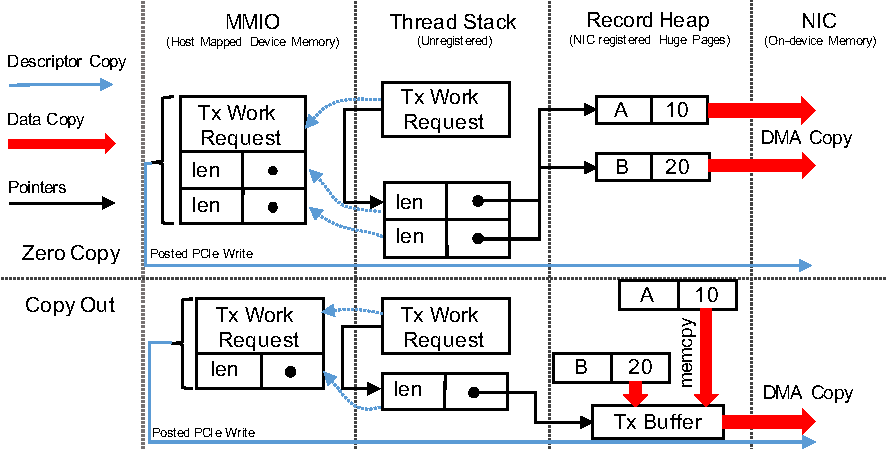
\includegraphics[width=\textwidth]{fig-mem-regions.pdf}
\caption{Key structures involved in network transmission.}
\label{fig:mem-regions}
\end{figure}

\begin{table}[t]
\def\arraystretch{1.25}%  1 is the default, change whatever you need
\caption{Experimental cluster configuration.}
\begin{tabular}{@{}l@{\hskip 12pt}l@{}}
\toprule
\textbf{CPU} & Intel Xeon E5-2450 (2.1~GHz, 2.9~GHz Turbo) \\
    & 8 cores, 2 hardware threads each \\
\textbf{RAM} & 16~GB DDR3 at 1600~MHz \\
\textbf{Network} & Mellanox MX354A ConnectX-3 Infiniband HCA (56 Gbps Full Duplex) \\
        & Connected via PCIExpress 3.0 x8 (63~Gbps Full Duplex) \\
%        & 7 Mellanox SX6036G FDR Switches \\
\textbf{Software} & CentOS 6.6, Linux 2.6.32, gcc 4.9.2, libibverbs 1.1.8, mlx4 1.0.6 \\
\bottomrule
\end{tabular}
\vspace{0.25eX}
\label{tbl:config}
\end{table}

\begin{figure}[t]
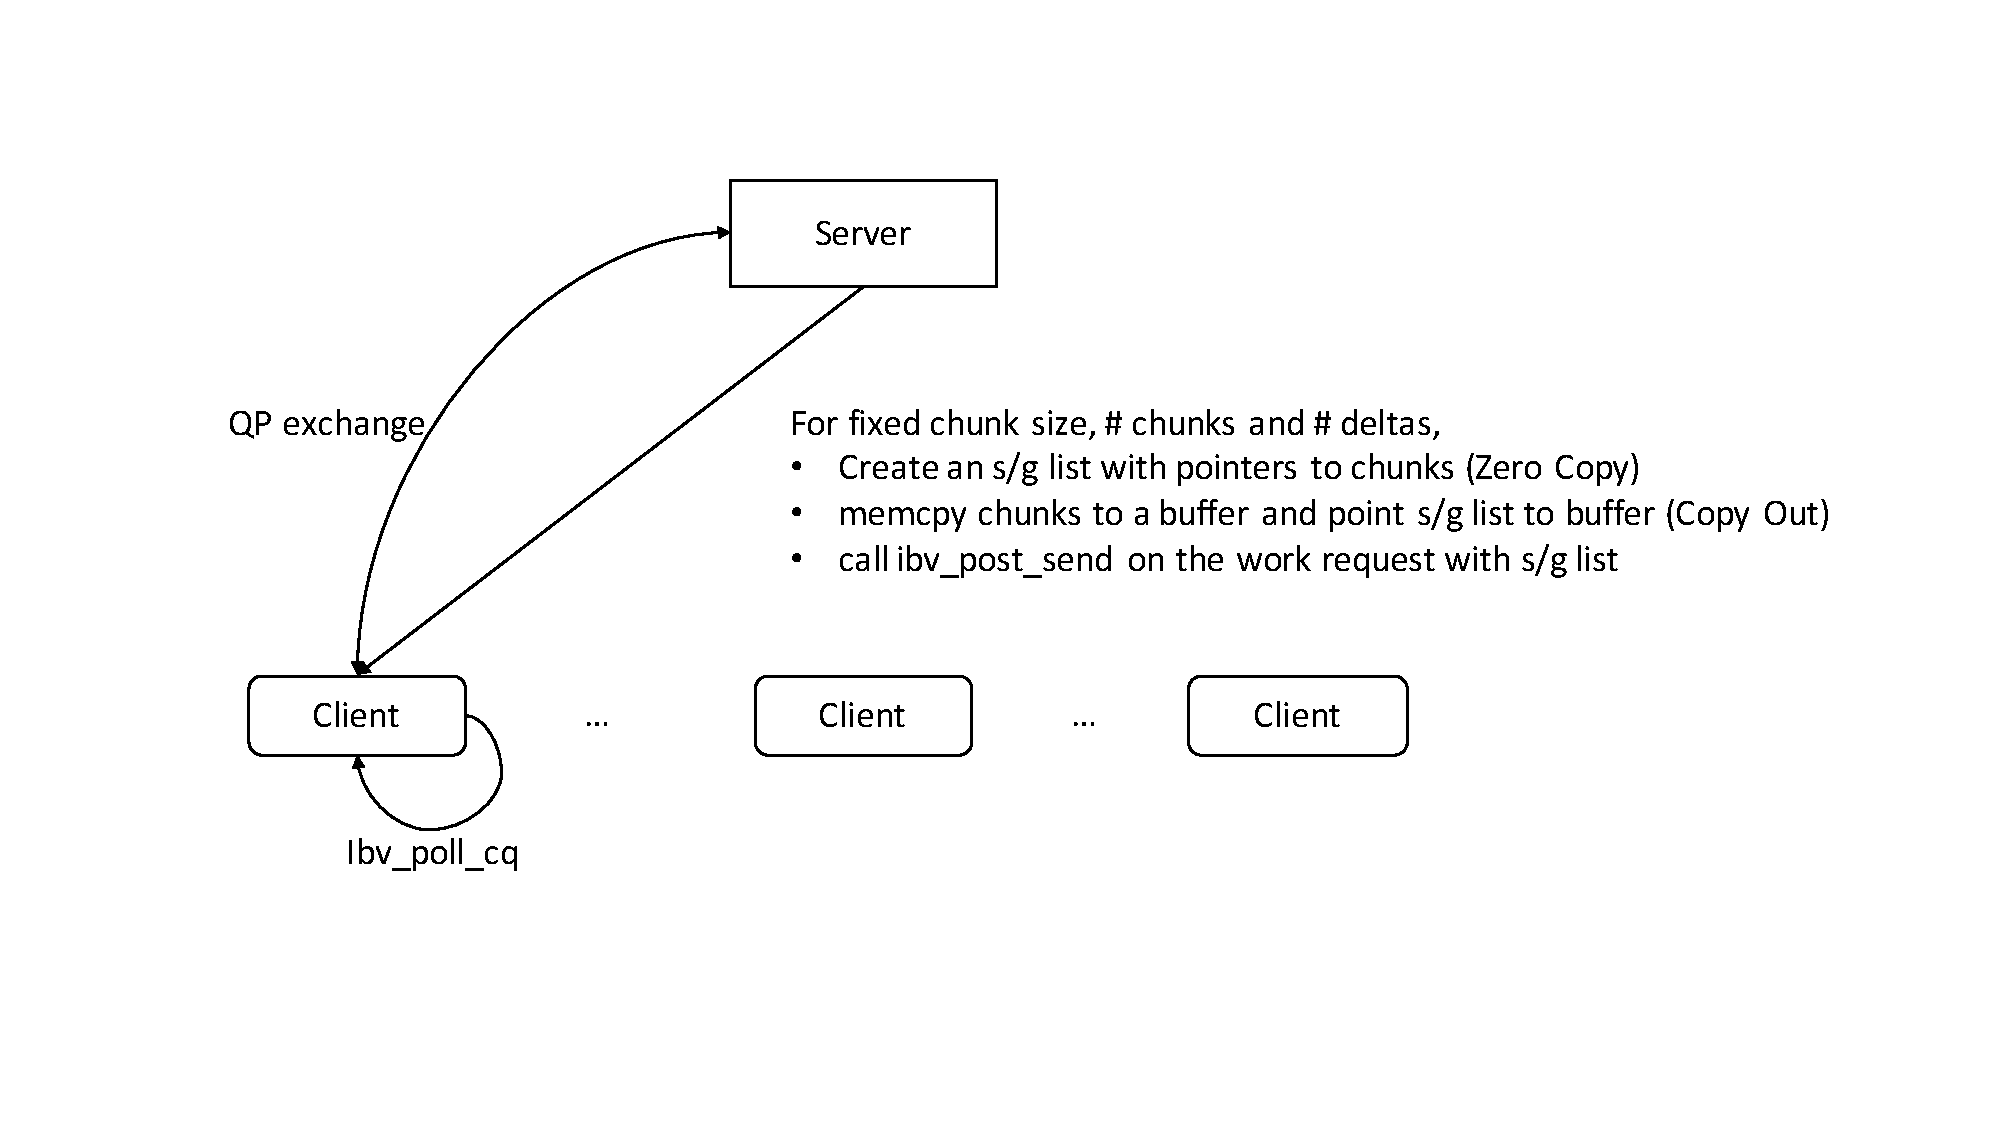
\includegraphics[width=\textwidth]{fig-setup.pdf}
\caption{Experiment setup. Each of the 15 clients communicate to a pinned thread on the server.}
\label{fig:setup}
\end{figure}

\begin{figure}[t]
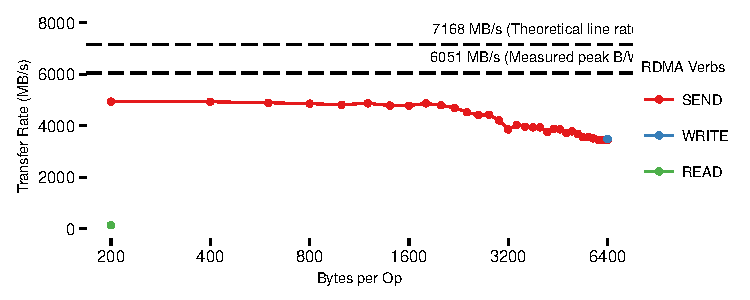
\includegraphics[width=\textwidth]{fig-200B-RDMAverbs}
\caption{Transmission rate for 200 B records over different RDMA verbs and 
varying S/G lengths. We only show \cpp{WRITE} at full capacity and \cpp{READ} at one read per transmission.}
\label{fig:200B_transrate}
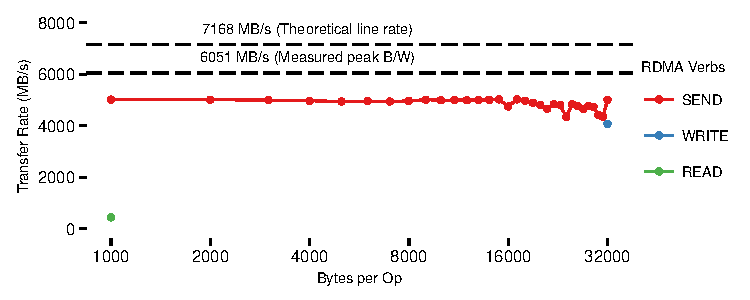
\includegraphics[width=\textwidth]{fig-1000B-RDMAverbs}
\caption{Transmission rate for 1000 B records over different RDMA verbs and 
varying S/G lengths. We only show \cpp{WRITE} at full capacity and \cpp{READ} at one read per transmission.}
\label{fig:1000B_transrate}
\end{figure}

\begin{figure}[t]
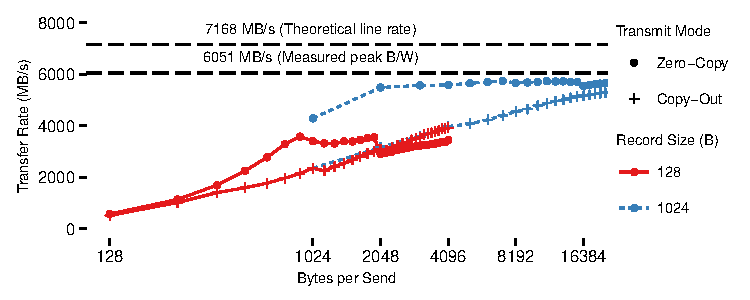
\includegraphics{fig-zero-copy-tput.pdf}
\caption{Transmission throughput for Zero Copy and Copy Out.}
\label{fig:zero-copy-tput}
\end{figure}

\begin{figure}[t]
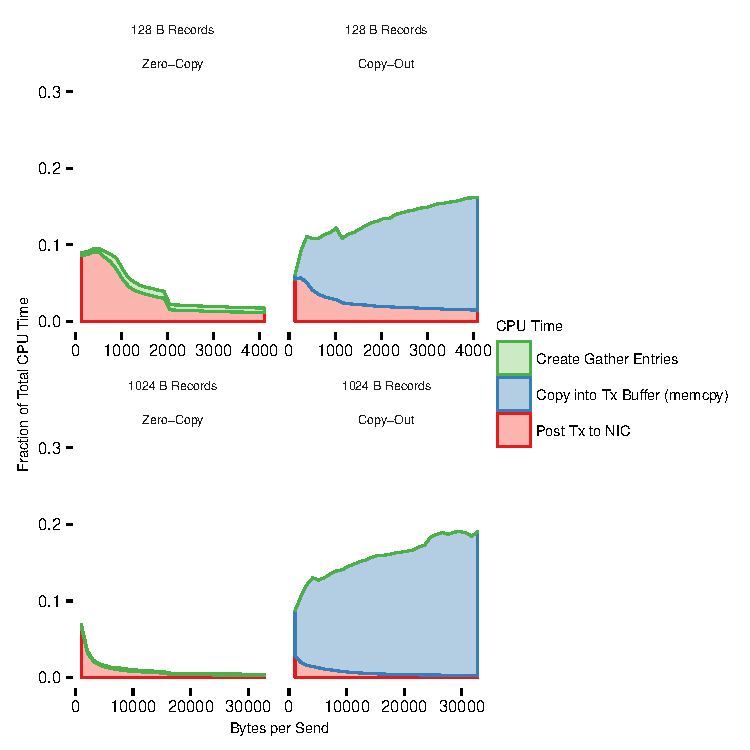
\includegraphics[width=\textwidth]{fig-overheads.pdf}
\caption{Breakdown of absolute CPU overheads for transmission.}
\label{fig:overheads}
\end{figure}

\begin{figure}[t]
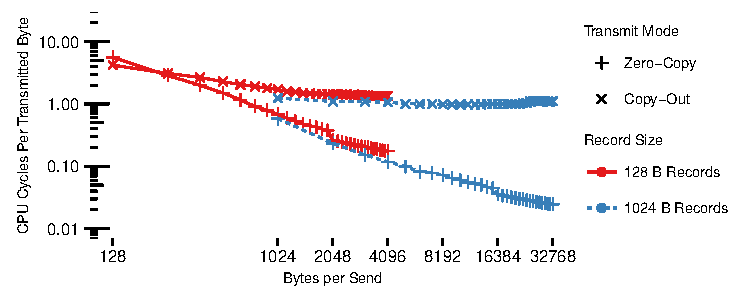
\includegraphics{fig-cycles.pdf}
\caption{Cycles per transmitted byte for large and small records with Zero Copy and Copy Out. Note the log-scale axes.}
\label{fig:cycles}
\end{figure}

\begin{figure}[t]
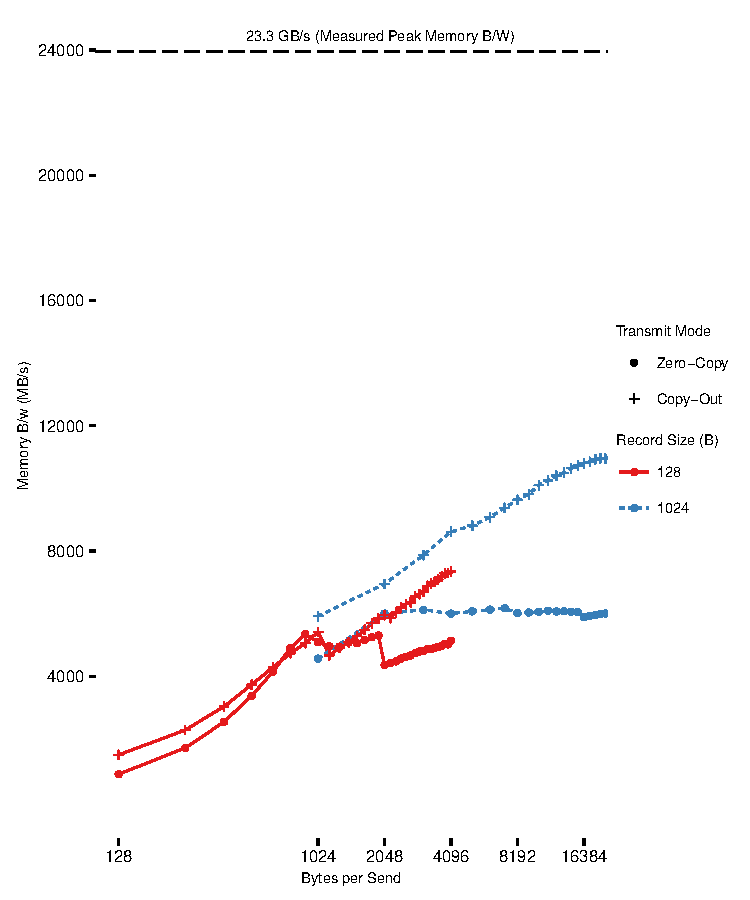
\includegraphics[width=\textwidth]{fig-membw.pdf}
\caption{Measured memory bandwidth impact on the system during transmission.}
\label{fig:membw}
\end{figure}

\begin{figure}[t]
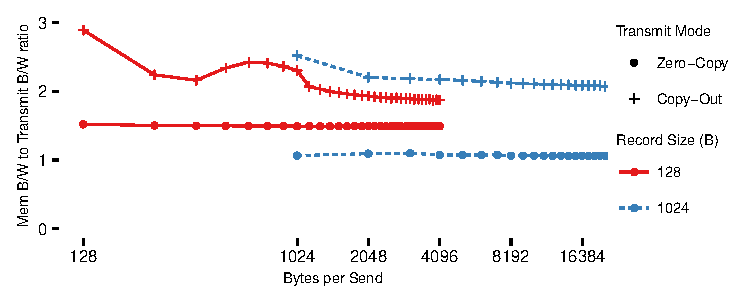
\includegraphics[width=\textwidth]{fig-membw-ratio.pdf}
\caption{Ratio of memory bandwidth to transmission throughput.}
\label{fig:membw-ratio}
\end{figure}

\begin{figure}[t]
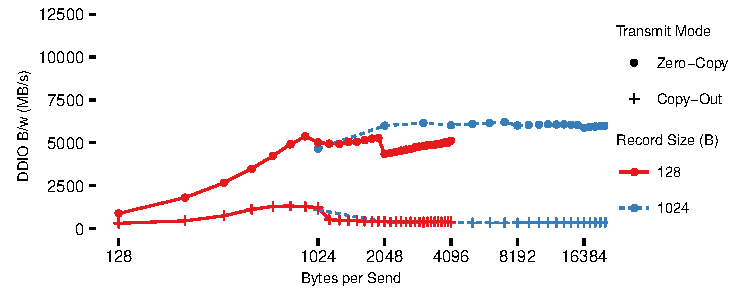
\includegraphics[width=\textwidth]{fig-ddiobw.pdf}
\caption{DRAM accesses (MB/s) LLC misses from DDIO. vs throughput.}
\label{fig:ddiobw}
\end{figure}

\begin{figure}[t]
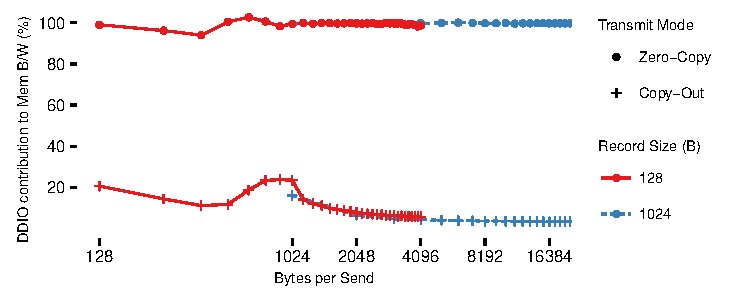
\includegraphics[width=\textwidth]{fig-ddiobw-percent.pdf}
\caption{Percentage of LLC misses that contribute to total memory bandwidth consumed.}
\label{fig:ddiobw-percent}
\end{figure}

\begin{figure}[t]
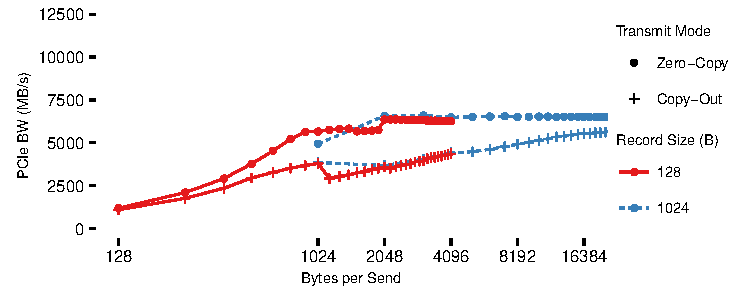
\includegraphics[width=\textwidth]{fig-pciebw.pdf}
\caption{DRAM accesses (MB/s) due to LLC misses due to PCIe.}
\label{fig:pciebw}
\end{figure}

\begin{figure}[t]
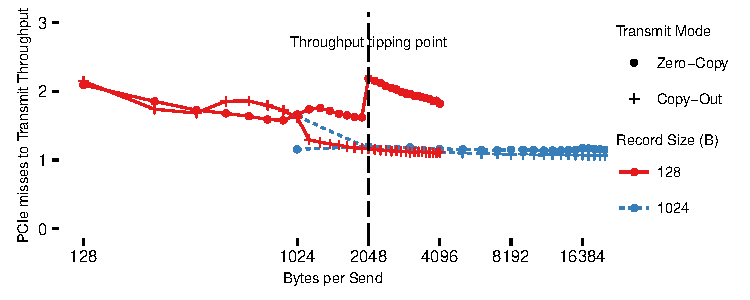
\includegraphics[width=\textwidth]{fig-pciebw-ratio.pdf}
\caption{Ratio of DRAM accesses because of PCIe to transmission throughput.}
\label{fig:pciebw-ratio}
\end{figure}


%%% -*-LaTeX-*-

\chapter{Applications for a Client-Assisted Design}
\label{chap:applications}

We have seen the impact of Zero Copy on network transmission and memory bandwidth and how that 
compares to using Copy Out to transmit data over the network. The difference
in throughput is explicitly seen for smaller 128~B records, where owing to the descriptor overhead and anomalies discussed 
in Chapter~\ref{chap:modernnics}, Copy Out gives better throughput performance especially when the transmissions get larger.
We have already established that 128~B records show a more realistic depiction of record sizes in the future
and that seems to be the growing consensus in the community~\cite{fb-memcache,fb-workload}. 

At first, the throughput results from comparing Zero Copy and Copy Out for 128~B 
records might tempt us to think that it is always better to use a Copy Out get maximum throughput with smaller records.
The complications of implementation and the cost of overheads are also rampant when using small records with Zero Copy.
The bigger problem with Copy Out might get overlooked in the face of all these issues surrounding Zero Copy.
While transmitting at around 5.9~GB/s (near line rate for the Connect-X3\textregistered NIC),
we saw that the memory pressure on the system is close to 12~GB/s, which is half of what we evaluated our server's total available memory bandwidth. 
This implies that network transmission will bottleneck available memory bandwidth for doing useful work such as processing data in a hybrid or analytical workload.

On-Line Analytical Processing (OLAP) and hybrid workloads composed of transactional and analytical queries have fuelled a renewed interest in column stores~\cite{cstore,cstorevsrowstore} in recent years. 
Column stores are uniquely positioned to take advantage of the NIC because of their layout and compression benefits.
 The impact of modern NIC while designing column stores should also be discussed for completeness. 

This chapter introduces a client-assisted design with bounded-disorder for using Zero Copy with no-update-in-place row stores as well as column stores. 
We evaluate the improvement in throughput and efficiency to provide evidence to back this approach.
We also make informed opinions on how Zero Copy might perform on column store designs 
for in-memory databases with co-operation from clients for materializing data.


\section{Bw-Trees}
Chapter~\ref{chap:modernnics} showed us that Copy Out might offer better transmission throughput for a large set 
of scattered small records. It also showed the perils of using Copy Out where it consumes a lot of memory bandwidth, 
starving the server of memory bandwidth that could be utilized for doing useful work.
Zero Copy promises memory bandwidth savings in addition to eliminating CPU overhead, 
while Copy Out can saturate the NIC throughput. We wanted to extract the best of both worlds, 
and we wanted to analyze structures that can uniquely take advantage of the 
Zero Copy paradigm. This would imply an arrangement of small records where the total transmission size 
goes up, helping the transmission throughput while being able to do Zero Copy to help reduce memory footprint. For this 
to work, we would also need a way of efficient update and synchronization so that data being fetched for transmission remain 
stable throughout the transmission.

Microsoft\textregistered Research came up with a modern B-tree structure called 
the Bw-Tree~\cite{bw-tree} which is their primary indexing structure for SQL Server Hekaton~\cite{hekaton}.
Bw-Tree is a highly performant, ordered index employing lock and latch free concurrency and effective utilization of caches in 
modern multicore processors. In the following sections, we explore how a client-assisted design involving a no-update-in-place 
structure such as Bw-Trees can take advantage of Zero Copy and gain maximum throughput 
without much system impact. We discuss how its lock freedom and delta records make it 
particularly suitable to exploit Zero Copy in the following sections. We then present
our evaluation of transmissions involving small records tacked on to bigger base records
to show the gains in throughput without consuming more memory bandwidth. 

\section{Lock-free Indexing}
\label{sec:bwtree-intro}
The Bw-Tree~\cite{bw-tree} is an atomic record store designed for extreme
concurrency. It is an ordered index that supports basic record create, update,
and delete (CRUD) operations in addition to searches and range scans.  It is
fully lock-free and nonblocking and is optimized for modern multicore
workloads. It can store to flash, but is also intended for in-memory
workloads; it serves as the ordered secondary index structure for the in-memory SQL
Server Hekaton~\cite{hekaton} engine.

In many ways, the Bw-Tree is a conventional paged B-link tree,
but it also has unique characteristics that interact with network-layer
design choices. Its lock freedom, its elimination of update-in-place,
and its lazy consolidation of updated records in virtual memory give it
tremendous flexibility in how query results are transmitted by the NIC.

Records may be embedded within leaf pages, or the leaf pages may
only contain pointers to data records. When used as a secondary index,
typically leaf pages would contain pointers, since otherwise, each record would
have to be materialized twice and the copies would need to be kept consistent.

The key challenge in a lock-free structure is providing atomic reads, updates,
inserts, and deletes without ever being able to quiesce ongoing operations (not
even on portions of the tree). Bw-Tree solves this problem by eliminating
update-in-place. All mutations are written to newly allocated memory; then
the changes are installed with a single atomic compare-and-swap instruction
that publishes the change.  Figure~\ref{fig:bw-tree} shows how this works.
In place updates are avoided by creating delta records ``off to the side'' 
that describe a logical modification to a page. Delta records are
prefixed to a chain ultimately attached to a base page.  When delta chains
grow long, they are compacted together with the base page to create a new base page.
All references to pages are translated through a mapping table that maps page
numbers to virtual addresses. This allows pages to be relocated in memory, and
it allows the contents of a page to swapped with a single atomic
compare-and-swap (CAS) operation.
\section{Delta Records}
\label{sec:deltarecords}
One of the key innovations of the Bw-Tree is its use of {\em delta records},
which make updates inexpensive.
Delta records allow the Bw-Tree to logically modify the
contents of an existing page without blocking concurrent page readers, without
atomicity issues, and without recopying the entire contents of the page for
each update.  Whenever a mutation is made to a page, a small record is
allocated, and the logical operation is recorded within this delta record. The delta
record contains a pointer to the page that it logically modifies. It
is then atomically installed by performing a CAS operation on the
mapping table that re-points the virtual address for a particular page number
to the address of the delta record.

Some threads already reading the original page contents may not see
the update, but all future operations on the Bw-Tree that access that page
will see the delta record. As readers traverse the tree, they consider
the base pages to be logically augmented by their delta records. Delta records
can be chained together up to a configurable length.  When the chain becomes
too long, a new base page is formed that combines the original base page
contents with the updates from the deltas. The new page is swapped in
the same way as other updates.

Read operations that run concurrent to update operations can observe superseded
pages and delta records, so their garbage collection must be deferred.
To solve this, each thread that
accesses the tree and each unlinked object are associated with a current {\em epoch}.
The global epoch is periodically incremented. Memory for an unlinked object can be
recycled when no thread belongs to its epoch or any earlier epoch.
The epoch mechanism gives operations consistent reads of the
tree, even while concurrent updates are ongoing. However, there is a
cost; if operations take a long time, they remain active within their epoch and
prevent reclamation of memory that has been unlinked from the data structure.


\section{NIC Implications for Bw-Tree}
Lock freedom has major implications on the in-memory layout of the
Bw-Tree. Most importantly, readers (such as the NIC DMA engine) can collect a
consistent view of the tree without interference from writers, and hold that
view consistent without stalling concurrent readers or writers to the tree.  This
natural record stability fits with the Zero Copy capabilities of modern NICs;
because the NIC's DMA engine is oblivious to any locks in the database engine,
structures requiring locking for updates would have to consider the NIC to
have a non-preemptible read lock for the entire memory region until the DMA completes.
Instead of copying records ``out'' of the data structure for transmission,
records can be accessed directly by the NIC. Eliminating the explicit copy of
the records into transmit buffers can save database server CPU and memory
bandwidth.

Page consolidation can also benefit the NIC and improve performance.  Records
in the Bw-Tree are opportunistically packed into contiguous pages in virtual
memory, but the view of a page is often augmented with (potentially many)
small delta records that are scattered throughout memory.
A database might save CPU and memory bandwidth by more
aggressively deferring or even eliminating consolidation of records into
contiguous regions of memory or pages. We show in
our evaluation that highly discontinuous data can slow
transmission throughput but that aggressive consolidation is inefficient; delta
records can dramatically reduce consolidation overheads while keeping records
sufficiently contiguous to make the NIC more efficient.
Overall, we seek to answer these key questions:
\begin{myitemize}
\item
When should records be transmitted directly from a Bw-Tree? Are there cases
where explicitly copying records into a transmit buffer is preferable to Zero Copy?
\item
How aggressive should a Bw-Tree be in consolidating records to benefit individual
clients and to minimize database server load?
\item
How does Zero Copy impact state reclamation in the Bw-Tree? Might long transmit
times hinder performance by delaying garbage collection of stale records?
\end{myitemize}



% Answering these questions?
% - When to tx zero copy versus not?
% - Show tx perf CPU use.


% K: Indexes in modern databases sustain million/op/s.

% K: To support extreme concurrency sometimes lock-free [cite BwTree, ART]

% K: Range scan performance key. But raises key question? How to inexpensively
% get the data to the NIC?

% K: Simplest approach: CO results and transmit. Tradtionally this would
% have yielded three copies. One into the results buffer, one for the kernel to
% copy the results into packet buffers, and one for the NIC to DMA the data for
% transmit.

% What about Zero Copy? Several problems:
%  - atomicity
%  - garbage collection and object lifetime
%  - packaging the objects for efficient transmit.
%    - pre-package? (paged structures)
%    - use NIC DMA engine?
% Key question? What are the gains?
%  - Reduced copies -> reduced memory bandwidth use, reduced CPU time

% K: Zero copy? Then data structure must be tied into messaging layer. Can work
% with epoch-based GC, but what about long scans? Could hold back GC and stall
% tree in the limit.




\section{Evaluation}

\subsection{Extending the Delta Format to Clients}


The experiments in Chapter~\ref{chap:modernnics} consider delivering a clean, ordered set of records to the
client. That is, the server collects and transmits the precise set of records
in the correct order, either via Copy Out or Zero Copy. Another option is to
transmit base pages along with their deltas and have clients merge the results.
This approach is attractive because it organically fits with the design of the
Bw-Tree and it suits the NIC's DMA engine well.  The NIC can transmit the
large contiguous base pages (16~KB, for example) with little CPU overhead.
It also eliminates Copy Out for small records, avoiding the ceiling of transmission throughput. %(\ref{Chnics-sec:zero-copy-tput}).
Merging records on the client side is cheap; the server can even append them to
the response in a sort order that matches the record order in the base page for
efficient $O(n)$ iteration over the records that requires no copies or sorting.


\subsection{Throughput and Efficiency of Delta Records}
\label{sec:delta-tput-efficiency}
Figure~\ref{fig:deltas-tput} shows the benefits of delta records. In our
experiment, each transmission consists of a single 16~KB base page while the
number (one to thirty one) and size (128~B and 1024~B) of the delta records attached to each transmission is varied.
The NIC benefits from the large base page, and it manages to keep the network
saturated. CPU overhead ranges from less than 0.3\% when there are a few delta
records up to about 0.6\% when there are more. This offers a 30$\times$ reduction 
in CPU overhead in comparison with our evaluation of the Copy Out approach in 
Section ~\ref{sec:overhead}. Compared to Zero Copy of scattered
small records, this approach also yields a 1.6$\times$ throughput advantage;
Figure~\ref{fig:zero-copy-tput} shows that throughput peaks around 3.4~GB/s when
records are scattered, while the delta format achieves around  5.6~GB/s. The main cost 
to this approach is the cost of consolidating delta records into new base pages 
when chains grow long; we consider this overhead in more detail in the next section.

% 5740/3532
% 1.62
% = 1.6x

\subsection{Tuning Page Consolidation}
\label{sec:consolidation}


Bw-Tree and many indexing structures are paged to amortize storage
access latency, and paging can have similar benefits for network transmission
as well. However, the user-level access of modern NICs makes interacting with
them much lower-latency than storage devices. This raises the question of
whether paging is still beneficial for in-memory structures. That is, is the
cost of preemptively consolidating updates into pages worth the cost, or is it
better to transmit fine-grained scattered records via Zero Copy or Copy Out?

%\begin{figure}[H]
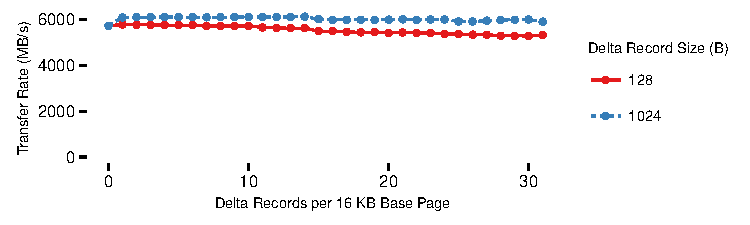
\includegraphics{fig-deltas.pdf}
\caption{Zero Copy transmit performance when transmitting using 
Bw-Tree like delta records}
\label{fig:deltas}
\end{figure}


% Regular CPU overhead
%    copied chunkSize chunksPerMessage   busyFrac
% 1       0       128                1 0.08386966
% 2       0       128                2 0.11668905
% 3       0       128                3 0.10951036
% 4       0       128                4 0.10252412
% 5       0       128                5 0.06622680
% 6       0       128                6 0.06367224
% 7       0       128                7 0.06985951
% 8       0       128                8 0.06227349
% 9       0       128                9 0.05706500
% 10      0       128               10 0.04953507
% 11      0       128               11 0.04680207
% 12      0       128               12 0.04342779
% 13      0       128               13 0.04162006
% 14      0       128               14 0.04048418
% 15      0       128               15 0.03841897
% 16      0       128               16 0.02195241
% 17      0       128               17 0.02131298
% 18      0       128               18 0.02084331
% 19      0       128               19 0.02049131
% 20      0       128               20 0.02022781
% 21      0       128               21 0.01989223
% 22      0       128               22 0.01952930
% 23      0       128               23 0.01917201
% 24      0       128               24 0.01921045
% 25      0       128               25 0.01872136
% 26      0       128               26 0.01838027
% 27      0       128               27 0.01814930
% 28      0       128               28 0.01809671
% 29      0       128               29 0.01792050
% 30      0       128               30 0.01771566
% 31      0       128               31 0.01749623
% 32      0       128               32 0.01781422


% Delta CPU overhead
%    copied deltaSize deltasPerMessage    busyFrac
% 1       0       128                0 0.004176226
% 2       0       128                1 0.004343818
% 3       0       128                2 0.004479262
% 4       0       128                3 0.004715360
% 5       0       128                4 0.004881293
% 6       0       128                5 0.004947248
% 7       0       128                6 0.005532234
% 8       0       128                7 0.005632129
% 9       0       128                8 0.005691837
% 10      0       128                9 0.005749774
% 11      0       128               10 0.005764381
% 12      0       128               11 0.005905733
% 13      0       128               12 0.006012879
% 14      0       128               13 0.006140493
% 15      0       128               14 0.006128670
% 16      0       128               15 0.004983695
% 17      0       128               16 0.005027644
% 18      0       128               17 0.005060442
% 19      0       128               18 0.005158658
% 20      0       128               19 0.005279367
% 21      0       128               20 0.005294916
% 22      0       128               21 0.005320413
% 23      0       128               22 0.005371369
% 24      0       128               23 0.005409892
% 25      0       128               24 0.005470040
% 26      0       128               25 0.005479338
% 27      0       128               26 0.005522727
% 28      0       128               27 0.005549651
% 29      0       128               28 0.005604431
% 30      0       128               29 0.005634841
% 31      0       128               30 0.005600399
% 32      0       128               31 0.005787729



The results of our earlier experiments help answer this question.  If Copy Out
is used to gain faster transmission of small records, then the answer is
simple. Even if every update created a complete copy of the full base page, the
extra copies would still be worthwhile so long as more pages are read per
second than updated. This is true for most update/lookup workloads and read-only
range queries make this an even better trade-off.

However, consolidation must be more conservative when using Zero Copy to yield
savings, since Zero Copy can collect scattered records with less overhead than
Copy Out. Yet there is a good reason to be optimistic.  Delta records
reduce the cost of updates for paged structures. If each base page is limited
to $d$ delta records before consolidation, the number of consolidations is
$\frac{1}{d}$. This means that allowing short delta chains dramatically reduces
consolidation costs, while longer chains offer decreasing returns. This fits with
the NIC's preference for short gather lists; allowing delta chains of length 4
would reduce consolidation by 75\% while maintaining transmit throughput that
meets or exceeds on-the-fly Copy Out.  The large 16~KB base pages also
improve transmit performance slightly, which improves efficiency.

For small records, transmitting compacted base pages that have a few deltas gives
a total CPU savings of about 10\%. For the same CPU cost, a server can perform
about 6.5~GB/s of page compaction or about 425,000 compactions per second for
16~KB pages. Even in the worst case scenario where all updates are focused on a
single page, delta chains of length four would tolerate 1.7~million updates per
second with CPU overhead lower than Copy Out. So, delta records can give the
efficiency of Zero Copy with the performance of Copy Out.


\subsection{Impact on Memory Bandwidth}
% Copy out max: 11596
% Delta max: 6226
Figure ~\ref{fig:deltas-membw} shows the total consumed memory bandwidth while 
transmitting records. It is interesting to note that regardless of the variation in 
delta record sizes, memory bandwidth stays roughly the same. Comparing Copy Out 
transmissions of similar size, we get a 46\% reduction in the consumption of 
memory bandwidth in the system. Another interesting factor is that the transmission 
involved only a few consolidated delta records, which we showed in Section~\ref{sec:consolidation} is 
beneficial; there is no added memory bandwidth pressure if we decide to transmit smaller 
or larger records. The bigger base page gets us to peak transmission, and a limited number of 
delta records is favored for aggregate CPU costs. We have arrived at the sweet spot of 
transmitting large amounts of data in a modern NIC.


\subsection{Impact on Garbage Collection}

Using Zero Copy tightly couples the higher level database engine's record
allocation and deallocation since records submitted must remain stable until
transmission completes. Fortunately, existing mechanisms in systems that avoid
update-in-place accommodate this well, like Bw-Tree's epoch mechanism described
in Section~\ref{sec:bwtree-intro}. Normally, the Bw-Tree copies-out returned records.
While an operation and its Copy Out are ongoing, the memory that contains records
that have been unlinked or superseded cannot be reclaimed. Zero Copy
effectively defers the copy until the actual time of transmission. As a result,
transmissions completions must notify the higher level database of transmission
completion to allow reclamation. This delay results in more latent garbage and
hurts the memory utilization of the system.

In practice, this effect will be small for two reasons. First, Zero Copy adds a
transmission, which completes within a few microseconds; however, it also saves a
\memcpy~ that accounts for 1~to~2~\textmu s for a 16~KB transmission. Second, the
amount of resulting data held solely for transmission should generally be
more than compensated for by eliminating the need for explicit transmit
buffers. With Copy out, the size of the transmit buffer pool is necessarily
larger than the amount of data under active transmission, and internal
fragmentation in the transmit buffers makes this worse.


\section{Zero Copy for Column Stores}

Column-oriented in-memory databases pose unique challenges in interacting with a modern NIC. 
Column stores use contiguous memory locations to store adjacent columns. They have also been known 
to use Run-Length Encoding, Dictionary Encoding, Bit-Vector Encoding, and heavier schemes 
like Lempel-Ziv Encoding for yielding better compression, which is one of the many value 
propositions of using a column-oriented layout. 

We observed in the previous  sections that Zero Copy offers promising performance if 
we had stable entries and used Zero Copy to transmit the results while responding to a range query. 
However, the fundamental problem lies in the fact that end-users expect query processing and analytics on data 
to materialize results in row-order. It has been argued before that early materialization of data
helps performance in column-oriented databases~\cite{cstore-material}. This makes the application 
of a scatter gather list difficult, and we might have already used a \memcpy ~or an alternative 
to materialize the data. 

We argue for the possibility of a different materialization strategy with more engagement from the 
clients. If the database server were to sent filtered columns and required metadata such as the 
dictionary encoding as scatter gather entries, we could leverage Zero Copy's performance. We believe 
this approach would work even for hybrid layouts~\cite{hyrise-hybridstores} that use row-oriented or 
column-oriented formats varying the width of columns according to the type of workload. Figure ~\ref{fig:rowstore-colstore}
shows how row stores and column stores could transmit data using Zero Copy using a client-assisted design.
In practice, there are numerous challenges associated with this design:
\begin{myitemize}
\item {\em Client co-operation}; this scheme of transmitting results would need smart clients that are 
capable of materializing data given the encoding scheme and the columns. We assume that the client 
has enough resources to spend in finessing the results.
\item {\em Low selectivity in queries}; we have seen packing more data yields more savings and performance 
from Zero Copy. We also know that the compression schemes in column stores can limit transfer sizes. 
As a result, queries with low selectivity are a natural fit for Zero Copy.
\item {\em Compressed metadata}; the client-assisted design would need the encoding to be transmitted
along with the results; this would need efficient compression and lean data structures for metadata.
\end{myitemize}
There needs to be further evaluation of how we can extract maximum performance and efficiency from 
a server equipped with a modern NIC.
\newline

\framebox[0.9\textwidth][c]{
  \parbox{0.7\textwidth}{
  \textbf{Takeaways: Client-Assisted Design with Delta Records}
  \begin{enumerate}
  \item Use of a large enough base page and updates as delta records helps in saturating NIC's transmission throughput.
  \item We get a 50\% reduction in memory bandwidth consumption using this approach without compromising transmission throughput.
  \item No updates in place and latch and lock freedom makes this approach clearly favorable for the modern NIC. 
  \end{enumerate}
  \textbf{Recommendation}: \textbf{Novel data structures can significantly influence the performance of a modern NIC}; To extract maximum performance from the NIC without compromising system resources, make use of client-assisted designs using lock-free structures that offer no updates in place.\label{takeaway:impact-bwtrees}
 }}


\section{Conclusion}
Zero Copy and Copy Out provides different optimizations for scattered, small records. A hybrid approach 
that leverages the high throughput that we obtain as a result of pre-assembling scattered records and 
using Zero Copy to transmit will yield good transmission throughput without consuming a lot of memory bandwidth.
\begin{myitemize}
\item With the assumption of {\em co-operative clients} and queries with low selectivity, we can continue 
to use Zero Copy and get better results while dealing with small, scattered records that are common in in-memory databases.
\item Advanced structures such as the Bw-Tree that allow no update in place and complete lock and latch freedom 
can be exploited for their suitability with the NICs. Further evaluation is required for these to work in practice.
\item Column stores could also benefit from the hybrid approach; materializing results in row-order makes Zero Copy 
more complicated in modern NICs and one possibility is to send the encoding metadata along with the results with client-assisted 
materialization.
\end{myitemize}
\newpage
\begin{figure}[H]
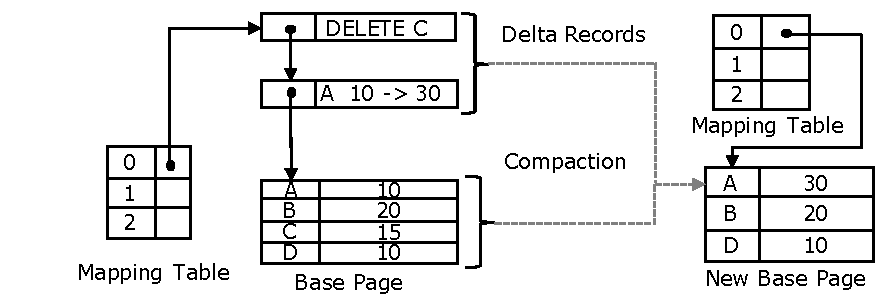
\includegraphics[width=\textwidth]{fig-bwtree.pdf}
\caption{ The structure of a Bw-Tree.}
\label{fig:bw-tree}
\end{figure}

\begin{figure}[H]
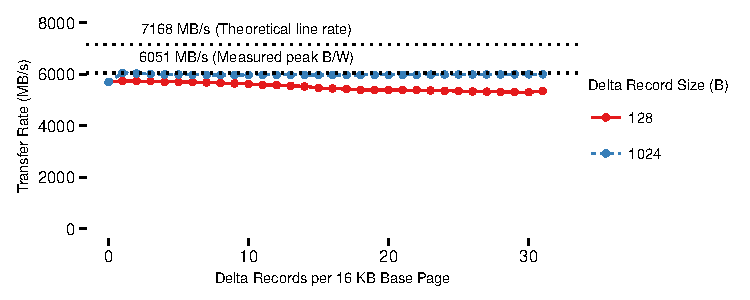
\includegraphics[width=\textwidth]{fig-deltas-tput.pdf}
\caption{Delta throughput}
\label{fig:deltas-tput}
\end{figure}

\begin{figure}[H]
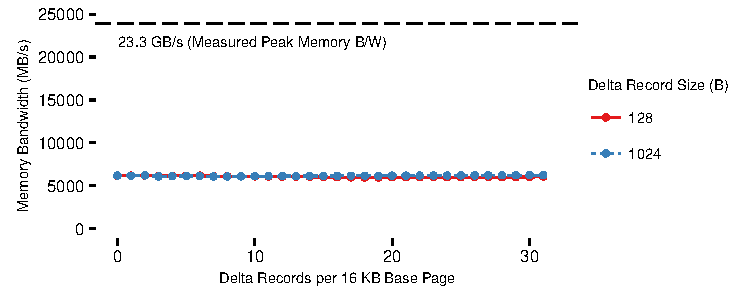
\includegraphics[width=\textwidth]{fig-deltas-membw.pdf}
\caption{Observed memory bandwidth impact varying delta records on a 16~KB base page.}
\label{fig:deltas-membw}
\end{figure}

\begin{figure}[H]
    \centering
    \begin{subfigure}[t]{0.4\textwidth}
        \centering
        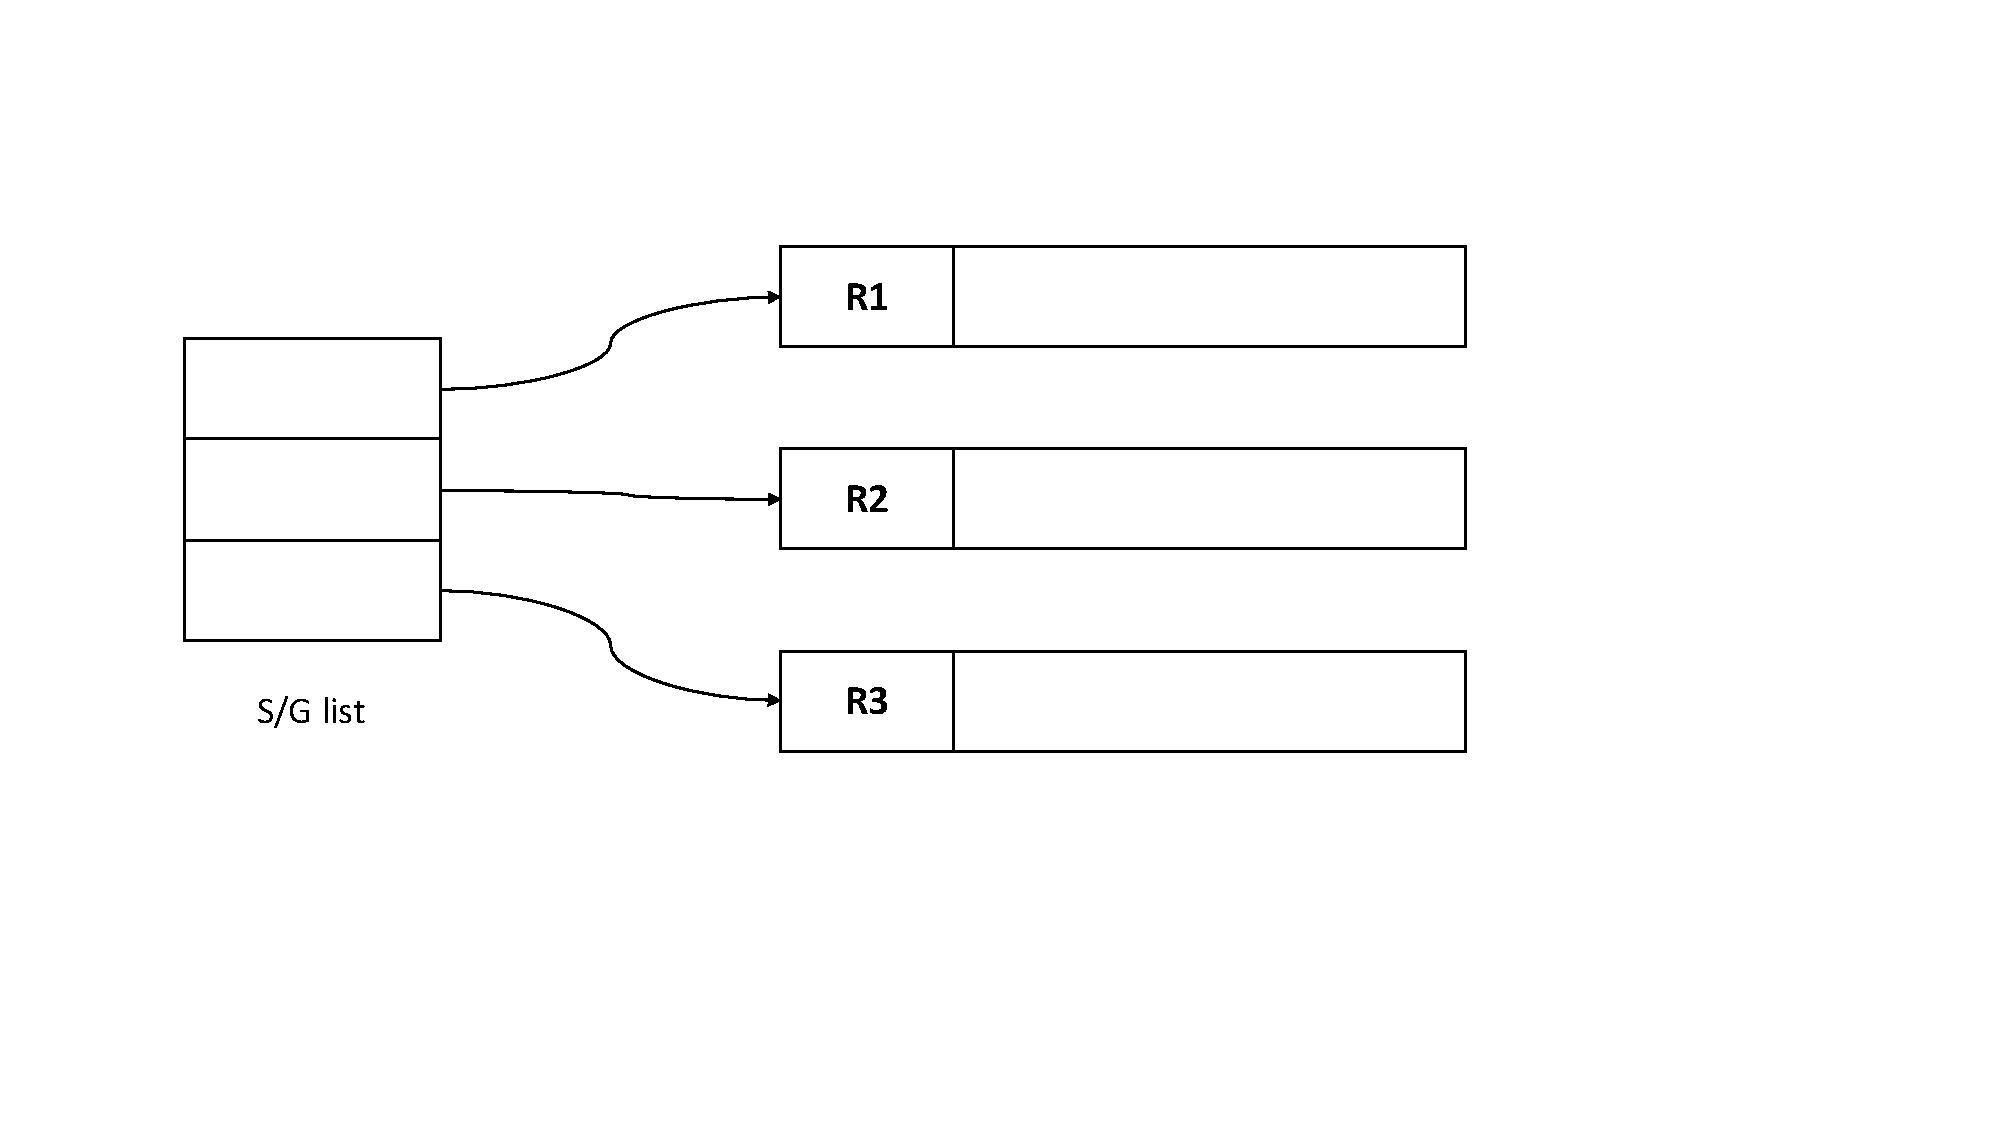
\includegraphics[height=1.5in]{fig-rowstore}
        \caption{Row-oriented Zero Copy}
    \end{subfigure}%
    ~ 
    \begin{subfigure}[t]{0.4\textwidth}
        \centering
        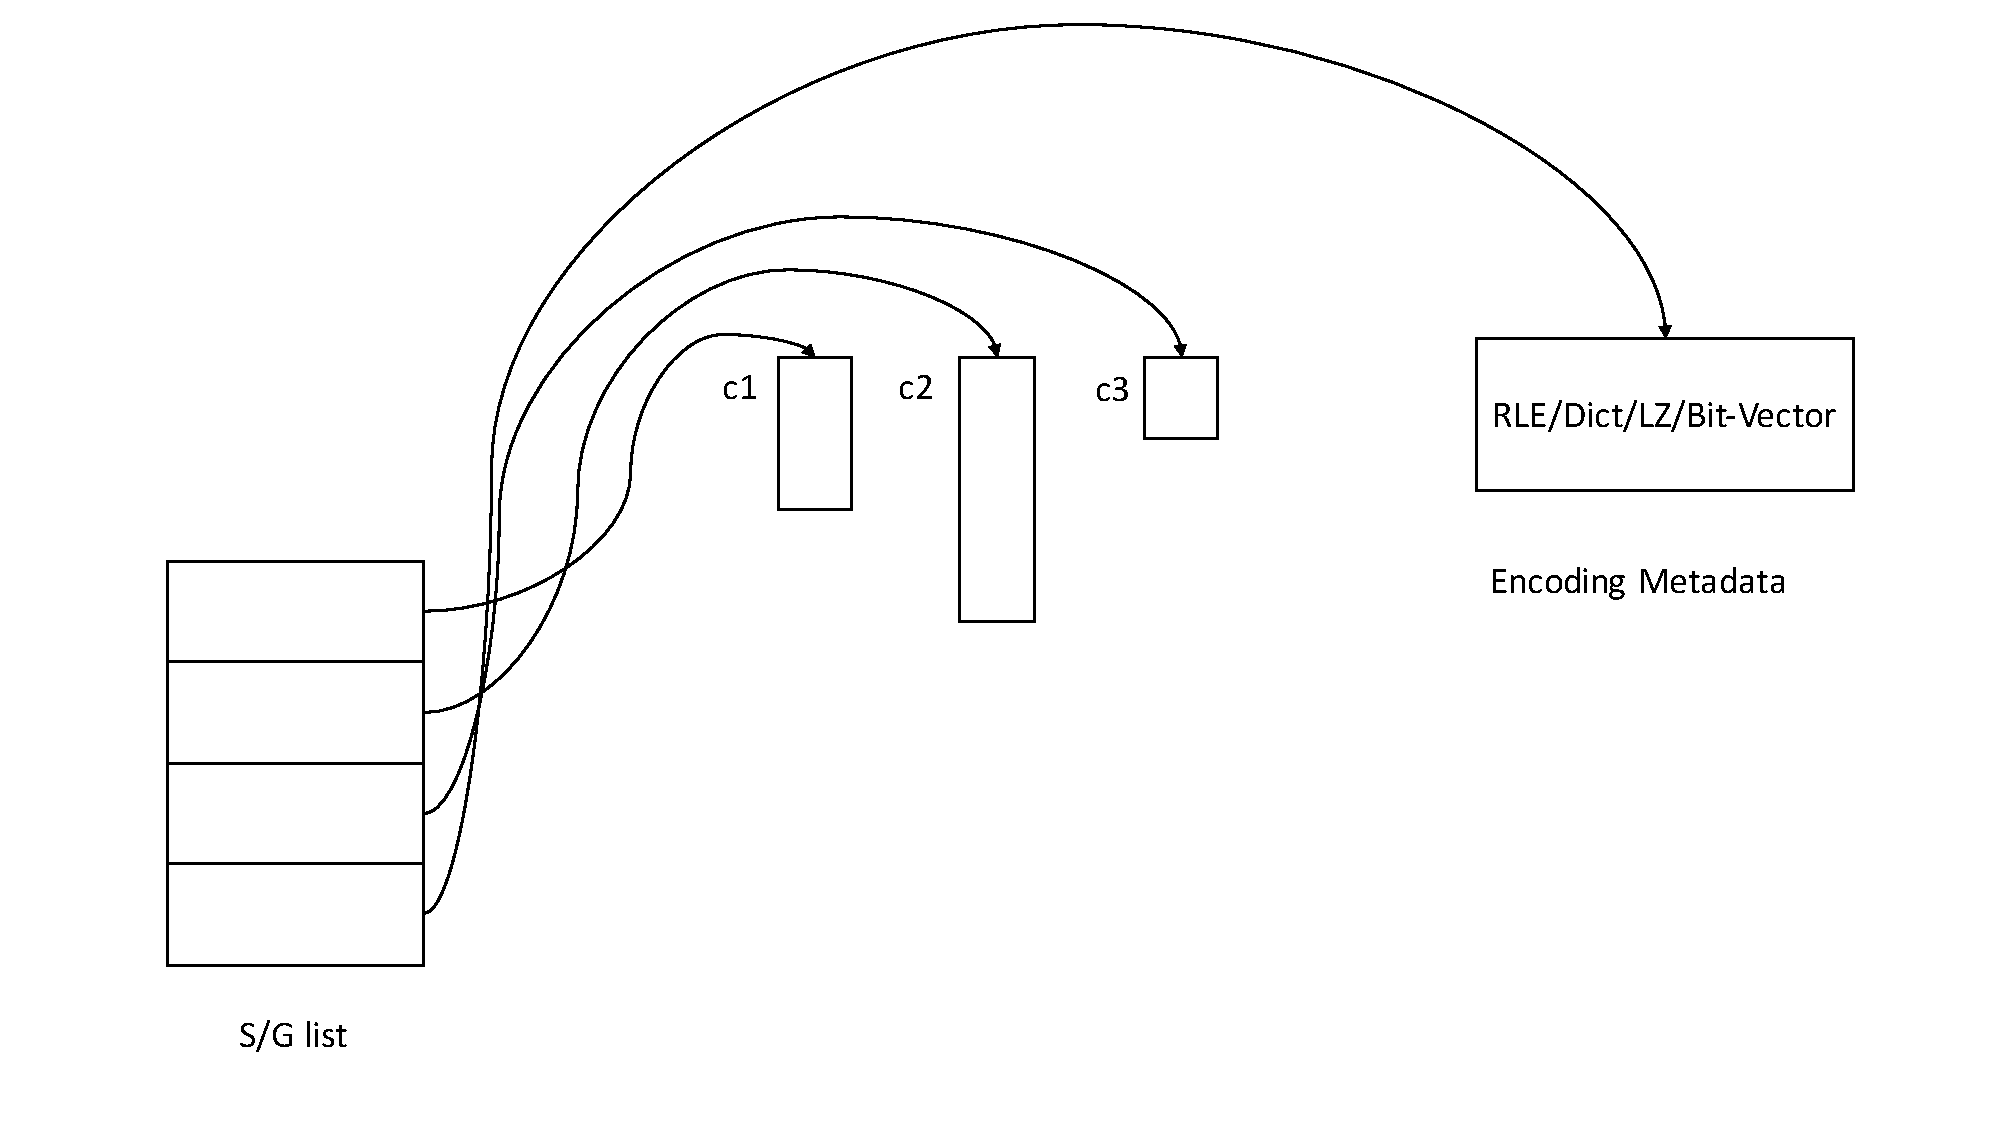
\includegraphics[height=1.5in]{fig-colstore}
        \caption{Column-oriented Zero Copy}
    \end{subfigure}
    \caption{Figure showing a possible design for Zero Copy on hybrid data layouts.}
\label{fig:rowstore-colstore}
\end{figure}

%  %%% -*-LaTeX-*-
\chapter{Pulling it all together}
This chapter summarises the key takeaways about modern NICs and our study of system impact while
transmitting at a very high data rate using them.

\framebox[0.9\textwidth][c]{
  \parbox{0.7\textwidth}{
  \textbf{Takeaways: Verbs}
  \begin{enumerate}
 \item \cpp{SEND} saturates NIC; can gather records and notify receiver when transmission completes.
 \item \cpp{WRITE} avoids invoking receiver; server must induce notifications some other way.
 \item \cpp{READ} is client initiated and avoids the server CPU in critical path; it's the lowest overhead on server,
  but can collect one contigous chunk per posted op, limiting its usefulness for returning complex responses.
  \end{enumerate}
  \textbf{Recommendation}: Use \cpp{SEND} primitives for returning scattered set of records. \label{takeaway:verbs}
 }}


\framebox[0.9\textwidth][c]{
  \parbox{0.7\textwidth}{
  \textbf{Takeaways: Throughput}
  \begin{enumerate}
  \item Bigger records can saturate the NIC; Zero Copy is significantly faster for bigger chunks.
  \item Zero Copy is limited by the length of S/G list; Zero Copy can't saturate the NIC transmitting 128~B records.
  \item Copy out can be faster for smaller records unless S/G length {\em is carefully tuned}; we examine Copy Out's efficiency in Section ~\ref{sec:overhead}.
  \end{enumerate}
  \textbf{Recommendation}: For large sets of small, scattered records, use Copy Out. If your record sizes are bigger, always use Zero Copy. \label{takeaway:tput}
 }}


\framebox[0.9\textwidth][c]{
  \parbox{0.7\textwidth}{
  \textbf{Takeaways: Breakdown of absolute CPU costs}
  \begin{enumerate}
  \item \memcpy ~dominates the CPU overheads in transmission; Zero Copy offers 8x savings for small records and 45x savings for larger records.
  \item Considerable CPU overhead means Copy Out is better at transmitting $<$384~B of data; For smaller records, overhead of adding and copying descriptors can't be ignored.
  \end{enumerate}
  \textbf{Recommendation}: If CPU overhead is the likely concern, use Zero Copy; adding an exception for this rule for transmissions $<$384~B might help minimising overheads. \label{takeaway:cpu-overhead}
 }}


\framebox[0.9\textwidth][c]{
  \parbox{0.7\textwidth}{
  \textbf{Takeaways: CPU Efficiency of Transmission}
  \begin{enumerate}
  \item Most efficient CPU utilization for transmission is obtained while using Zero Copy on large batches; 72\% savings for 128~B records and 95\% savings for 1024 B records.
  \item Zero Copy is 2x costlier than Copy Out in transmitting a single 128B record; results like equality searches on small records might be better served by Copy Out.
  \item If the results to be transmitted involve 2 or more records, Zero Copy is always more CPU efficient.
  \end{enumerate}
  \textbf{Recommendation}: Zero Copy effectively offloads CPU and cost per byte goes down drastically when you transmit larger batches of records. \label{takeaway:cpu-cycles}
 }}


\framebox[0.9\textwidth][c]{
  \parbox{0.7\textwidth}{
  \textbf{Takeaways: Impact of Memory Bandwidth}
  \begin{enumerate}
  \item Copy Out might occupy significant portion of available memory bandwidth; Transmissions of 32 records of 1~KB size consumed \textbf{half of all available bandwidth}.
  \item Smaller records have a smaller memory footprint and may not affect available bandwidth; The trend follows transmission throughput and there are areas where Zero Copy is costlier.
  \end{enumerate}
  \textbf{Recommendation}: Zero Copying larger records saves the most memory bandwidth while giving stellar throughput. \label{takeaway:impact-membw}
 }}


\framebox[0.9\textwidth][c]{
  \parbox{0.7\textwidth}{
  \textbf{Takeaways: Intel\textregistered Data Direct I/O}
  \begin{enumerate}
  \item While doing Zero Copy, almost all of the misses from DDIO region result in reads issued to memory controller.
  \item While doing Copy Out, since the data is already in memory, A miss from the DDIO region may not always result in a memory read.
  \end{enumerate}
  \textbf{Recommendation}: Keeping your transmission sizes under the size of a modern LLC (~20MB) can lower your memory bandwidth consumption considerably. \label{takeaway:impact-membw}
 }}


\framebox[0.9\textwidth][c]{
  \parbox{0.7\textwidth}{
  \textbf{Takeaways: Copy Out side effects of DDIO}
  \begin{enumerate}
  \item The additional \memcpy ~ step prefetches data to LLC at a cost and improves the number of DDIO misses that result in DRAM accesses. 
  \item If not for the DDIO effects, we would have seen a bigger drop in throughput and memory efficiency for Copy Out. 
  \end{enumerate}
  \textbf{Recommendation}: DDIO paints a slightly different picture of memory consumption favoring Copy Out; in the bigger scheme of things, total memory bandwidth consumed still makes us prefer Zero Copy. \label{takeaway:impact-ddiobw-savings}
 }}


\framebox[0.9\textwidth][c]{
  \parbox{0.7\textwidth}{
  \textbf{Takeaways: DRAM accesses due to PCIe traffic and anomaly in Throughput}
  \begin{enumerate}
  \item The memory utilization because of PCIe peaks as transmission throughput drops for small records doing Zero Copy.
  \end{enumerate}
  \label{takeaway:impact-membw}
 }}


\framebox[0.9\textwidth][c]{
  \parbox{0.7\textwidth}{
  \textbf{Takeaways: Client-Assisted Design with Delta Records}
  \begin{enumerate}
  \item Use of a large enough base page and updates as delta records helps in saturating NIC's transmission throughput.
  \item We get a 50\% reduction in memory bandwidth consumption using this approach without compromising transmission throughput.
  \item No updates in place and latch and lock freedom makes this approach clearly favorable for the modern NIC. 
  \end{enumerate}
  \textbf{Recommendation}: \textbf{Novel data structures can significantly influence the performance of a modern NIC}; To extract maximum performance from the NIC without compromising system resources, make use of client-assisted designs using lock-free structures that offer no updates in place.\label{takeaway:impact-bwtrees}
 }}

%%%% -*-LaTeX-*-
%Evaluation has been folded into other chapters as per Ryan's suggestion.
%%% -*-LaTeX-*-

\chapter{NIC Aware Reconfiguration}
\label{chap:migration}
We have seen that the current generation of NICs are capable of transferring Gigabytes of 
data per second in latencies of the order of a few microseconds. We have reasons to believe 
that the next generation of networking hardware will have the ability to process 
hundreds of millions of messages per second at bandwidth of the order of tens of Gigabytes per 
second and sub-microsecond latencies~\cite{cx6}.
We saw from the previous chapters how the nuanced performance characteristics of 
a modern NIC will influence overall transmit performance and server resource utilization 
for large data transfers such as responses to range scans. Another pressing 
concern for a modern in-memory database operating at scale is quick reconfiguration. 
Since DRAM is the most expensive resource in a modern cluster, efficient rebalancing 
involves fast reconfiguration that is frugal on resources and keeps the impact on their 
SLAs minimal. Informed with our lessons about the NIC, it is reasonable to assume that protocols for reconfiguration 
today can benefit from these optimizations and armed with the changes for proposed protocol, data migration might come 
closer to what the hardware is capable of doing today.

In this chapter, we discuss the state-of-the-art migration protocols and their 
performance, do an analysis of the existing migration protocol in RAMCloud, 
and armed with the lessons learned by profiling a modern NIC, we make concrete 
suggestions on how a new protocol might be well poised to take advantage of the 
new hardware.
\section{State-of-the-Art}
% Squall 10.a 5~MB/s calculation
% 10 GB database, divided over 4 nodes; that’s 2.5 GB per node
% Now scale down from 4 to 3, that’s 2.5 GB / 3 per node
% So 833 MB of data coming in
% Takes (220 - 30) = 190 s
% 833 MB / 190 S


Fast reconfiguration of in-memory data is something that has been overlooked largely
by the research community. There have been novel techniques for live migration of 
key value stores such as Albatross~\cite{albatross} that provides unavailability windows 
as short as 300ms, Zephyr~\cite{zephyr} that does on-demand pulls, and asynchronous data 
pushes to minimize failed transactions and unavailability for migration while operating 
at transactional latencies of 50~ms. Squall~\cite{squall} went further with fine-grained 
partitioning with optimizations such as prefetching. Squall also offers minimal overhead 
to their transactional latencies, which are of the order of tens of milliseconds and migrate 
data overall at the rate of around 5~MB/s (Refer to Squall paper, Figure 10 a). While these efforts offer reconfiguration speeds 
better than other systems and minimal addition to their millisecond latencies, that is far 
from what a modern NIC is capable of delivering. From our benchmark, we knew that the NIC 
can deliver transmission throughputs of around 5~GB/s while operating at microsecond latencies. 
There are important lessons to take from these recent research efforts on migration, but without 
devoting attention to the NIC and its complex performance characteristics, today's cluster of
storage servers cannot offer migration performance order of magnitudes better than the state-of-the-art.

\section{Migration in RAMCloud}
We saw from the previous section what the latest reconfiguration protocols are capable of doing and how they can only 
offer 1000$\times$ less throughput than the latest NICs operating under millisecond latencies. There is a different class of systems~\cite{ramcloud,farm,rdmabillion,herd} that 
were developed recently that optimizes for end-to-end latency and has the ability to perform millions of operations 
per second per server. RAMCloud~\cite{ramcloud} is a prime example of such a system that promises median read latencies 
of 5\textmu~s and responds to workloads up to a million operations per second. These characteristics result from the fact that 
these systems were designed from the ground up keeping low latencies in mind and any significant disruption to their operating 
latencies might deem them less useful. RAMCloud has a migration protocol that offers around 100MB/s data transfer speeds albeit 
synchronous and unpipelined. While this is faster than other systems, we believe that carefully leveraging the NIC, 
we can attain better throughput without compromising on latency.

\subsection{Current Protocol}
Figure ~\ref{fig:migration-current} shows the steps involved in the existing protocol. The key drawback to the current approach is that 
most of the steps involved are synchronous and blocking. The current protocol could make use of Zero Copy since migration usually involves a 
large amount of data and sets of large data and the presence of \cpp{safeVersion}~\cite{ramcloudtx} makes Zero Copy an interesting proposition 
for migration in RAMCloud. While doing migrations, we found that the migration throughput that RAMCloud's existing protocol provides to 
be around 150 MegaBytes per second (MB/s). While this is at least ten times better than the state-of-the-art, there is definitely room for improvement in the protocol.
We profiled the time spent in migration doing each of the steps mentioned in Figure~\ref{fig:migration-current}.

Figure~\ref{fig:bottlenecks} shows an analysis of how each of the bottlenecks affects RAMCloud's migration performance. We made versions of migration 
protocol bypassing each of the bottlenecks and measured RAMCloud's migration performance in each of those scenarios. We migrated a table of a hundred million 
records with record sizes of 100~Bytes, which comes close to 9~GB including the key and metadata.

The first bottleneck we bypassed was the re-replication of data to the backups. This is a configurable parameter and removing this, we observed a speedup from around 150~MB/s to around 
200~MB/s. This explains that while disk bandwidth was indeed a bottleneck, avoiding it does not give significant performance boost while migrating a small data set.

The second bottleneck we tried to avoid was to skip replaying the migrated segments on the receiver. From here on, the safety of the protocol is heavily compromised even under 
 nonfailures. Since the point of the experiment was to show how much each step contributes to overall performance, we discard safety. Skipping replaying segments took us from 
 200~MB/s to 600~MB/s. 

Since we exhausted all steps involved in the receiver during migration, we skipped the actual transmission of data from source to destination and not surprisingly, the throughput 
only went up from 600~MB/s to 700~MB/s. 

The final step is the most interesting with respect to the lessons we have learned by analyzing the NIC. Skipping the copying step before transmission took us from 700~MB/s to 
1150~MB/s. This underlines our earlier observation that any extra copy involved in a transmission is pure overhead and significantly affects performance. 
The analysis tells us that there is clearly room for improvement in migration performance in RAMCloud. While sequential replay of migrated segments of data seems to give the most benefits, 
it is safe to assume that use of Zero Copy while transmitting data from the source will enhance network transmission throughput without hurting the available memory bandwidth.

\subsection{Locality in RAMCloud}
RAMCloud's take on data locality is unique. RAMCloud promises uniform median latency of around 5\textmu s~\cite{ramcloud}. RAMCloud does not have a strong notion of collocating data across servers. 
It is known that transactions~\cite{ramcloudtx} and secondary indices~\cite{slik} can benefit with collocation of data. RAMCloud's data is hash partitioned, and within a server, the in-memory log is organized 
in a temporal order. We might be tempted to think that storing data in contiguous memory location in some order based on primary or secondary keys or even some other predetermined order will give better NIC performance. 
The key obstruction to doing this is RAMCloud's log cleaning mechanism~\cite{ramcloudfast}. RAMCloud's design philosophy rightly highlights the importance of DRAM utilization when all data is in memory. 
As a result, the log cleaner is designed in such a way that after cleaning, the log is reorganized so that records that are accessed in the same frequency are placed together; this makes sure that the records in the same 
segment get garbage collected together freeing up more space than otherwise. To keep this property intact, we cannot force a deterministic order of data in RAMCloud and this might turn out to be a problem if 
we want to pre-aggregate data to get higher transmission throughput.

We set up an experiment to demonstrate the effect of collocating data in RAMCloud. RAMCloud is slated to provide a throughput of one million operations per second. We set up a cluster of 10 RAMCloud servers 
and had ten clients issue ``multiget'' requests to the servers that return values for multiple keys in one operation. The operations were done on a table of 10 keys that were placed in various servers in different 
configurations. 

Figure~\ref{fig:colocation} shows the results of this experiment. When we had all 10 keys per table localized in each of the servers, the whole cluster is expected to produce a throughput of 100 million objects read per second.
Owing to the overhead of multiget, we observe around 45 million combined operations on the server. The dotted line shows the throughput of the server if we were to use a regular ``get'' request to extract keys one by one.
We see a great benefit in the total throughput when all keys are collocated in a single server for all tables. The x-axis indicates the server spread. When we move along the x-axis, the second point indicates a configuration where for every table, 9 keys belong in one server and 
another belongs to a different server. The right most point is the configuration where each server hosts one key of all the 10 tables across the server. The bottom half explains what fraction of total CPU burned was spent 
doing useful work (worker) and what fraction went into handling the communication between servers (dispatch). 
We can clearly see that the amount of useful work done takes a great hit while the communication overhead dominates 
even if each server in the cluster had to do one cross-machine extraction of data. Add this to the fact that if all the keys were evenly spread across the cluster, the ``multiget'' request does more harm than good and getting the 
keys one by one would have resulted in better aggregate throughput of the cluster. We can conclude that the effect of locality of data is paramount, and any movement of data to achieve better locality of data between servers will yield 
great performance later.
\section{Design Guidelines for a New Protocol}
Based on the analysis of the bottlenecks in the current protocol and the motivation that comes from having data localized to servers, some guidelines for developing a protocol for migration in RAMCloud
are given below that have ties to the lessons we learned from benchmarking a modern NIC.

\begin{myitemize}
\item Make use of {\em Zero Copy}; RAMCloud supports a slew of network transport protocols including TCP and Infiniband. Since kernel by-pass is essential in the design philosophy that calls for minimal 
interrupts, more popular packet processing oriented transports like DPDK~\cite{dpdk} are also supported. No matter what protocol is used, we have seen from our previous chapters that 
using Zero Copy yields superior performance and efficient utilization of resources. The new protocol should minimize the number of copies involved in transmission.

\item Layout your data such that there is {\em at least one large enough chunk} before transmission; Assuming we are doing a live migration while servicing data, it makes sense to reapply the guidelines 
from our evaluation of delta records in Bw-Trees here. Data could be pre-aggregated into a buffer
 and updates and some set of scattered records (limited by the network card) may be 
 transmitted, giving near line rate throughput and minimal overhead to consumed 
 memory bandwidth. Refer to Section~\ref{sec:delta-tput-efficiency} for how a 16KB 
 base page can enhance transmission throughput by 1.6 times.

\item {\em Defer re-replication} to the end; Our analysis of experiments only showed a minor increase of performance when we avoided re-replication. 
Larger migrations would need higher {\em disk I/O bandwidth}, which gets bottlenecked at around 
300MB/s for regular spinning disks. It would be ideal to defer re-replication to the end or use RDMA to achieve re-replication 
provided there is some way to ensure the safety of data in the face of failures during migration.

\item {\em Defer partitioning} decisions before migration; We mentioned that ordering data within a RAMCloud server is not feasible because of utilization. Any new migration scheme should continue to adhere to the principle of assuming no locality 
of data within the server before migration unless significant changes are made to the log cleaning mechanism.

\item {\em Parallelise or pipeline} steps in migration; We saw from our analysis that the sequential nature of the migration is detrimental to its performance. A new protocol should be 
able to parallelise the transfer of data as well as replaying at the receiver in order to attain maximum performance. 

\end{myitemize}
\newpage

\begin{figure}[H]
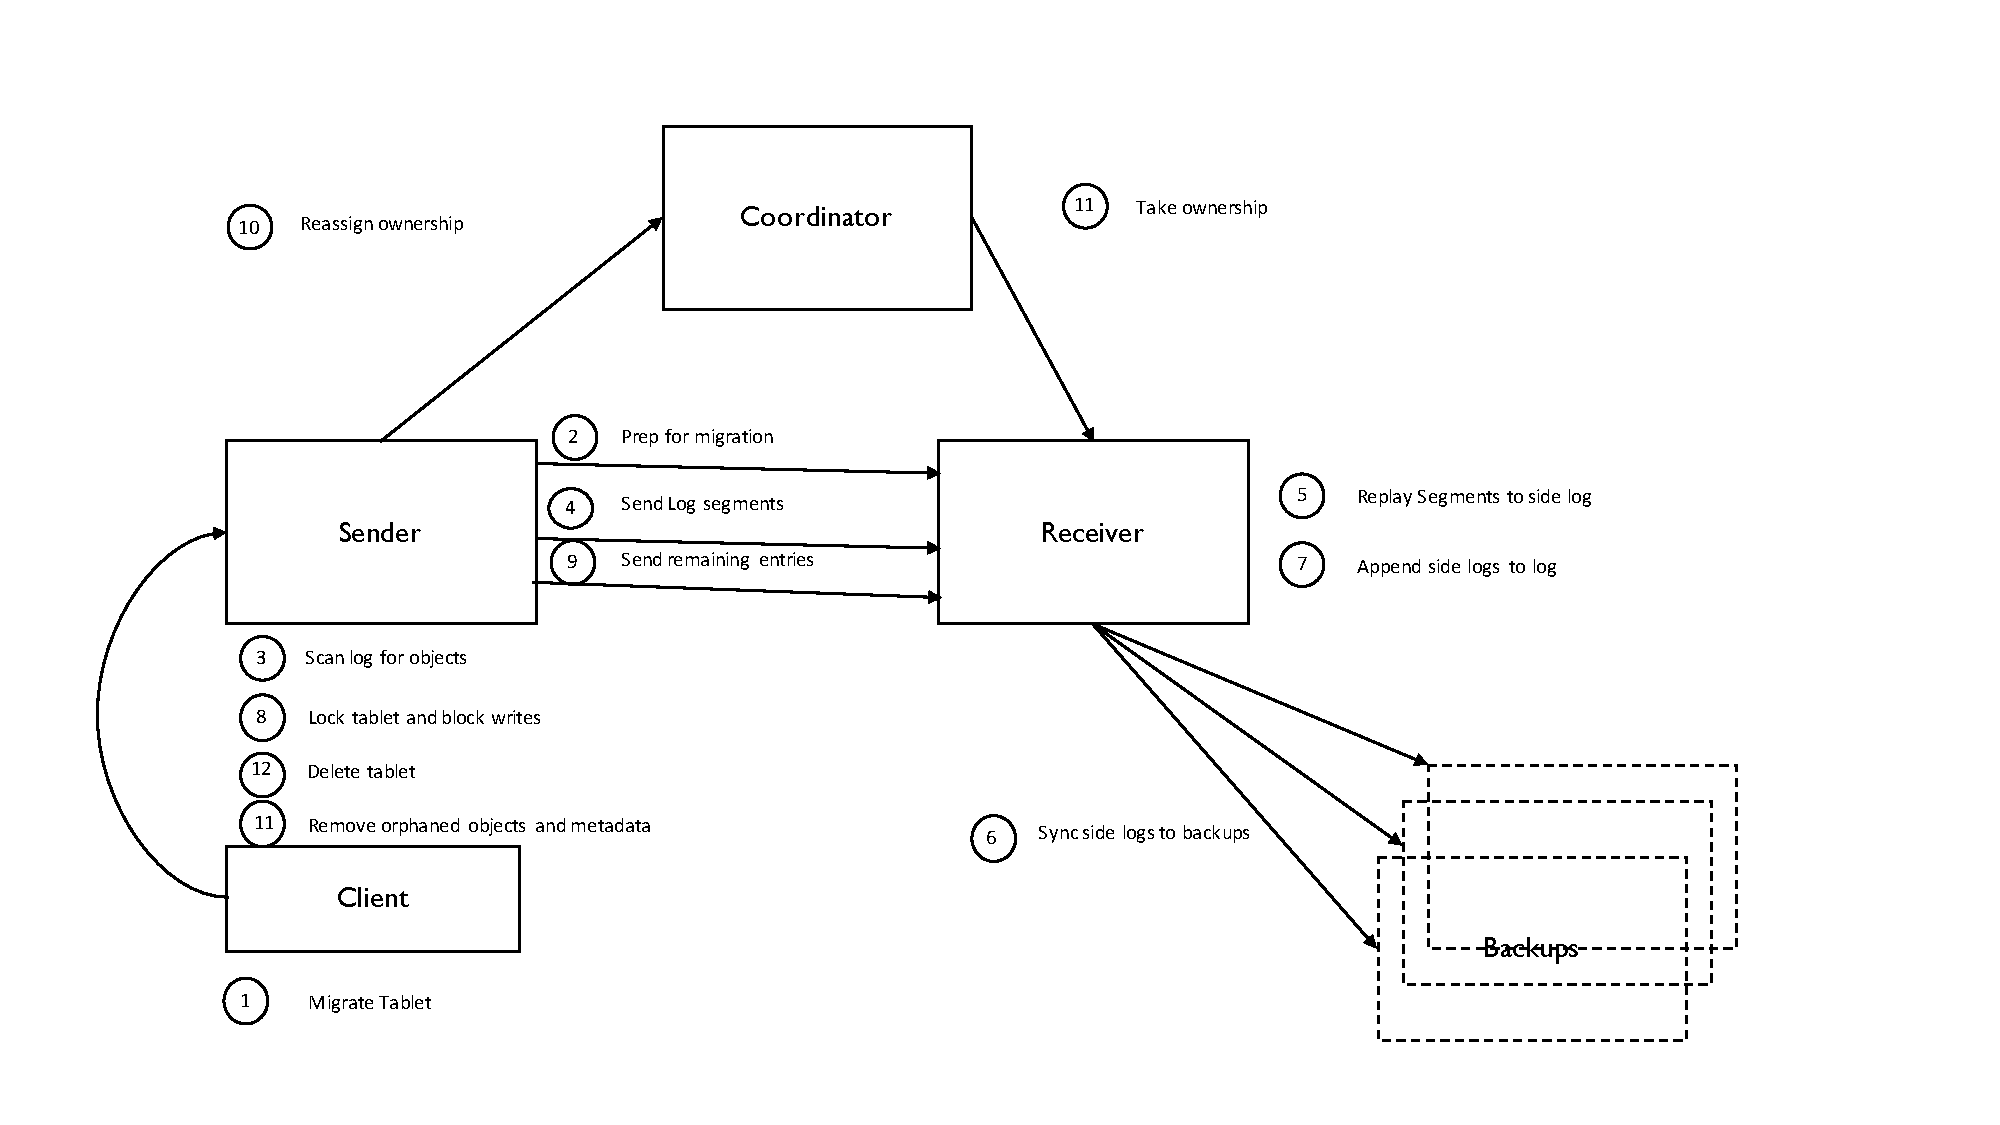
\includegraphics[width=\textwidth]{fig-current-migration.pdf}
\caption{Diagram showing steps involved in the current migration protocol of RAMCloud.}
\label{fig:migration-current}
\end{figure}

\begin{figure}[H]
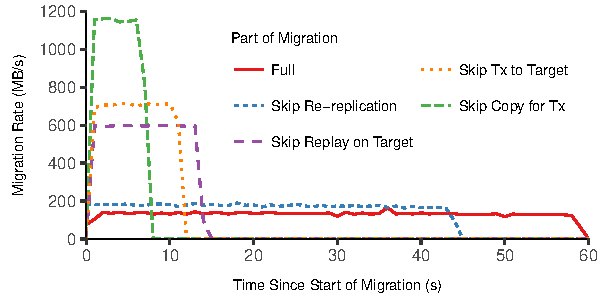
\includegraphics{fig-bottlenecks.pdf}
\caption{Analysis of bottlenecks in RAMCloud's current migration protocol.}
\label{fig:bottlenecks}
\end{figure}

\begin{figure}[H]
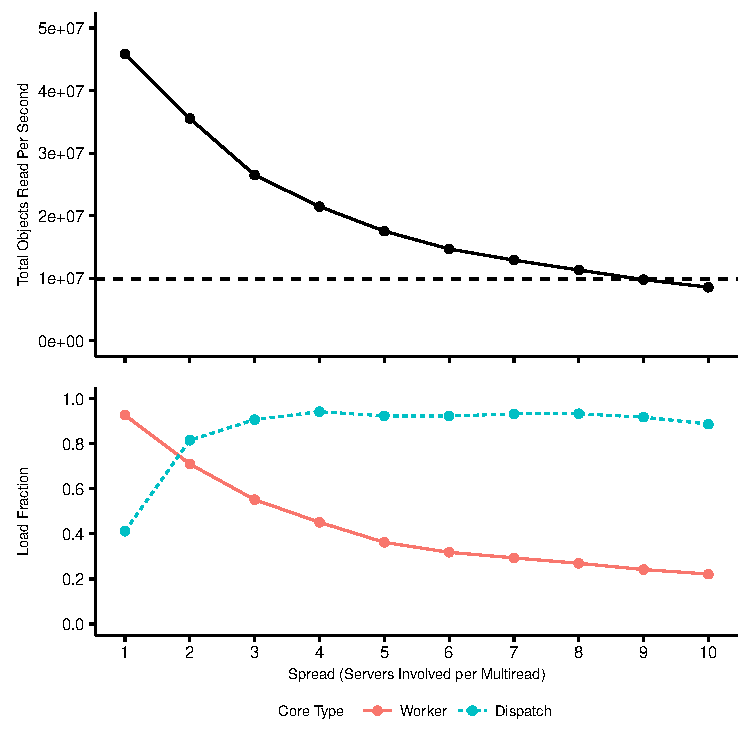
\includegraphics{fig-colocation.pdf}
\caption{Colocation plot. Collective throughput and fraction of useful work and communication overhead 
over server spread.}
\label{fig:colocation}
\end{figure}


%%% -*-LaTeX-*-

\chapter{Related Work}
\label{chap:relatedwork}

In-memory databases and low latency networks are very heavily researched areas
these days. Our work borrows concepts from numerous efforts both current and 
prior from the databases, networking, and operating systems research communities.
RAMCloud~\cite{ramcloud} itself was a research product built on top of other 
work on log-structured file systems and kernel by-pass networking. RAMCloud gave the 
world a distributed fast crash recovery, scalable log structured DRAM storage, and a new consensus 
algorithm~\cite{ryan-thesis,ongaro2011fast,ramcloudfast,raft} in addition to many other 
functionalities that makes it one of the most feature complete low latency storage systems 
to come out of research.

\section{In-memory Databases}
In-memory databases sparked a new wave of systems research in the 
networking and database communities. For a long time while developing storage
systems, researchers did not diverge from the  tried and tested model for the 
locality of reference. Conventional ``secondary storage" devices
such as disks were the final resting place of ever-growing amounts of managed data. With the 
enhanced requirements of scale by the popularization of Web 2.0 in the early 2000s, 
database designers created a caching layer of RAM in front of disks
to combat abysmal disk access times that were dragging down performance at scale. Memcached~\cite{memcached-orig}
is one such popular system and its further development
enabled it to operate at a scale of billions of operations per second on trillions of items~\cite{nishtala2013scaling}.

Another orthogonal area of research was to completely store all data in main memory.
This was made possible in the late 2000s by the evolution of DRAM technologies and declining cost of main memory.
Questions about durability and cost of replication 
were responded to by means of distributed recovery~\cite{ongaro2011fast} and advances in defragmentation techniques~\cite{ramcloudfast} 
ensured high DRAM utilization. Another recent development was in the acceptance of high throughput and low latency networks. 
Pioneered by the high performance computing community, these advanced networking fabrics 
such as Infiniband~\cite{pfister2001introduction} became more commonplace in 
data center networks, and kernel by-pass networking was made ubiquitous by packet processing 
frameworks such as DPDK~\cite{dpdk}, which enabled them to operate over universally accepted protocols
such as Ethernet. These developments have led to a deluge of storage systems research~\cite{mmdbmstutorial} 
exploring multiple verticals. Among the particularly notable ones are RAMCloud~\cite{ramcloud},
FaRM~\cite{farm}, and H-Store~\cite{hstore} (scale-out memory stores) and
MICA~\cite{mica}, HyPer~\cite{hyper}, and HERD~\cite{herd} (focused on single node performance).
While each of these systems has been driven by different dimensions 
of research, they all share the same concerns of in-memory storage systems 
operating on high-speed networks.

Today's main memory database systems offer a plethora of features that are at par with traditional
database systems including structured storage and indexing, concurrency control and transactions,
 durability and recovery techniques, query processing and compilation, support for high availability, and 
ability to support hybrid transactional and analytics workloads~\cite{mmdbmstutorial}.
FaRM~\cite{farm} is an in-memory, distributed computing platform that leverages lock-free reads over RDMA~\cite{rdma},
collocating objects and function shipping to provide performance characteristics of the 
highest order for an in-memory database. FaRM scales distributed transactions to
hundreds of millions of operations with recovery times of the order of milliseconds by relying on 
full replication in DRAM. There are other systems such as Silo~\cite{silo} that effectively utilize multicore CPUs.

\subsection{Column Stores}
Column-oriented databases have generated interest in recent years owing to the growing 
need of running complex analytical queries over a large amount of data. Most enterprise 
database solutions today ship with the column stores. This new focus has resulted 
in advanced materialization strategies and compression schemes~\cite{cstore,cstorevsrowstore,cstore-material,cstorecompression}.
In-memory databases with hybrid layouts~\cite{hybridinmemorycolstore} and other recent work on in-memory column stores~\cite{inmemorycracking} 
focus a lot on analytical workloads and techniques like database cracking~\cite{databasecracking} for adaptive indexing. 
MonetDB~\cite{monetdb} made significant milestones in OLAP processing of in-memory column stores. HyPer~\cite{hyperhybrid} 
is an example of a system that underlines the importance of RDMA in the context of a column store.


\subsection{Lock Freedom}
Lock freedom is important for Zero Copy and RDMA since the NIC also introduce contention 
since records are transmitted directly from their original memory location without an 
additional copy. Lock and latch freedom are 
design philosophies perfected on previous work on fine-grained concurrency 
primitives~\cite{finegrained} and lock-free hash tables ~\cite{lockfreeht}. Lock freedom is commonly
used in databases these days~\cite{htm} since they gained practicality by the common use of
epochs-based reclamation~\cite{lockfreedom} . 
More recent iterations of SQL engines such as Hekaton~\cite{hekaton} are 
examples for in-memory optimized  database engines. Bw-Tree~\cite{bw-tree}, a 
data structure that is lock and latch free, follows a no-update-in-place philosophy to indexing.
Others have worked on exploiting Hardware Transactional Memory~\cite{htm-old}
for in-memory transaction processing~\cite{drtm} as well as lock-free indexing~\cite{htm}.

\section{RDMA in Databases}
The merits of RDMA have been widely accepted by database researchers by now. The 
ability to offload CPU from transmission make it appealing while the necessity for 
multiple round trips to fetch data made people hesitant. The ability of Infiniband NICs to 
use scatter gather to assist remote memory access has also been discussed before~\cite{zerocopy04}.
From the early arguments~\cite{rdmacase} calling for the need for offloading CPUs to 
research aiming for a billion key value operations on key value servers ~\cite{rdmabillion},
RDMA seems to be a promising paradigm for the future of large-scale databases. Others have suggested
a decoupled server I/O architecture using Programmable I/O (PIO) and re-architecting virtual 
memory systems for network transfers~\cite{hicamp}. Key value stores
such as HERD~\cite{herd} and MICA~\cite{mica} and systems that provide more complex
data models such as RAMCloud~\cite{ramcloud} use RDMA effectively and there have been 
published guidelines to maximize performance for dispatch-heavy workloads~\cite{rdma}.

\section{Data Migration}
Research efforts focussing on reconfiguration for in-memory databases have seen a lot of 
interest lately. Albatross~\cite{albatross} offered live reconfiguration with unavailability windows as low as 
300ms. Zephyr~\cite{zephyr} focuses on mitigating violations to Service Level Agreements (SLAs) and limits 
change in average latency to 10-20\% but like Albatross, operates on latencies of the order of tens of milliseconds.  
Squall~\cite{squall} employs reactive pulls and pre-partitioning
of data for fast migrations and is the state-of-the-art for low impact migrations that specifically work well for 
heavily skewed workloads. Like others, Squall also operates on platforms with throughput and latencies orders of 
magnitude less than what is possible with today's hardware. The key challenge in implementing migration in a system 
like RAMCloud is to maintain the latencies that are 1000$\times$ tighter than these systems.

\section{Data Transfer in Fast Networks}
As pointed out by various researchers in the past, the days of slow networks are over~\cite{slow} 
and network no longer remains the primary bottleneck that database designers should take for granted.
This thesis argues heavily in favor of that fact. Several efforts in the past have exploited
user-level NIC access as well as RDMA for highly performant distributed database systems~\cite{ramcloud,farm,farmtx,drtm,hyper}
as well as block I/O for file systems~\cite{rdmagfs}. The closest analysis that we have found on 
range queries and in-memory databases~\cite{zerocopyrangequery} argues for use of RDMA reads and 
multisocket parallelisation of copying of data. Our analysis is more detailed and quantifies the 
results with memory bandwidth and effects of DDIO.
Our findings should also complement other efforts such as transactional key value stores~\cite{deuteronomy} 
and shared-data databases~\cite{tell}. Small, fixed-size request/response cycles have been optimized in
existing research~\cite{farm,herd,mica,rdma,ramcloud}, but the efficient
transmission of larger responses like range query results or data
migrations has been less well studied. Studies focused on large transmissions
have so far been limited to relatively static block-oriented data.
Our work focuses on optimizing transmission of large and complex query
results, which differs from these two categories. 

A complementary study by Kalia, Kaminsky, and Andersen~\cite{rdma} provides a
different analysis of host interaction with Mellanox Infiniband network adapters,
and they extract rules of thumb to help developers get the best performance from the hardware.
The low-level nature of their analysis is especially suited for
optimizing dispatch-heavy workloads with a high volume of small
request-response operations. While most of RDMA research prefers one-sided RDMA verbs, more recent efforts have shown 
the benefits of two-sided RDMA and datagram RPCs~\cite{fasst}. We believe that 
two-sided RDMA and RPC semantics are the most promising in today's architecture. In the future, 
richer semantics that allows the gathering of remote data might prove beneficial for one-sided RDMA verbs.


\section{Summary}
Our work is built on the premises of a lot of research ideas and its unique take on
heavy transfers in the presence of tight SLAs (latencies of the order of 10s of microseconds)
make it stand out among the related work. Until now, mixing workloads such as range scans 
and data migration, especially in the context of modern networks, has not been well
 understood from the server side. We present an in-depth analysis of resource utilization, 
 the impact of DDIO and how data layout affects performance and efficiency in a modern 
 in-memory database.

%%% -*-LaTeX-*-

\chapter{Conclusion}
\label{chap:conclusion}
Section~\ref{sec:contributions} remarked the following thesis statement:

``Scale-out in-memory stores are optimized for small requests
under tight SLAs, and bulk data movement, for rebalancing and range queries, interfere;
the thesis argues \linebreak carefully leveraging data layout and advancements in modern NICs
will yield gains in performance and efficiency for large transfers in these systems
without disrupting their primary obligations.''
 

We have found conclusive evidence for this statement by evaluating the transmit performance 
of a NIC and the resource utilization of a server while transferring large amounts of data. We 
made numerous recommendations and observations from benchmarking the NIC. We presented a client-assisted 
approach that will get better throughput without compromising resources. We analyzed the effect of collocating
data in RAMCloud and benchmarked the key bottlenecks in the current migration protocol. We also proposed a set of design 
guidelines for a new migration protocol for RAMCloud, drawing lessons from observing the NIC closely while it was 
transferring gigabytes of data. 

While evaluating the various RDMA primitives, we found that one-sided RDMA verbs, though they offload destination CPU, 
require additional acknowledgment mechanisms. We also found that client-initiated \cpp{READ}s cannot use the 
scatter gather DMA engine effectively. We arrived at the conclusion that \cpp{SEND} primitives 
are the most suited for returning scattered set of records.

We analyzed the transmission throughput of Zero Copy and Copy Out for 128~B records and found that bigger records can saturate the NIC.
Zero Copy is significantly faster for bigger chunks. Zero Copy is also limited by the length of S/G list for small 128~B records.
We also found that Copy Out can perform better if you have more records. We arrived at the following conclusion that 
unless your records are small and scattered, always use Zero Copy; for small and scattered records, you might need to tune your layout 
to get Zero Copy advantage.

Zero Copy with two-sided RDMA promises CPU savings by offloading CPU from the critical data transfer path of the sender. We found that 
CPU overheads in transmissions are largely due to the additional copies involved in Copy Out and Zero Copy benefits from avoiding the extra copy.
 
CPU efficiency of transmission is better measured in cycles spent per transmitted byte. We see that even transmitting two records at a time makes 
Zero Copy more CPU efficient in transmission and the gains get bigger for bigger transmissions.

Memory bandwidth is a crucial resource in an in-memory database server bound by DRAM capacity and latency. We found that for transfer of large 
records, the pressure on the memory controller is approximately 2X the transmission throughput and while transmitting at the line rate of our NIC, 
the server consumed half of all available memory bandwidth. If memory bandwidth is not an expendable resource, we ascertain that the designer should 
always use Zero Copy.
  
Intel\textregistered's recent micro-architectures have support for DDIO that treats LLC as the source and destination for I/O transfers. This has a significant impact on 
the memory pressure exerted to the system, especially for Copy Out. DDIO paints a slightly different picture favoring Copy Out since the cost of prefetching the data is 
paid up front; we do not incur additional misses from DDIO. This is less relevant in the bigger scheme of things and Zero Copy still wins in terms of total 
consumed memory bandwidth in the server
  
The transmission throughput anomaly where the throughput of Zero Copy is limited while transferring a large set of small scattered records is best explained to 
our knowledge with PCIe errors tapering off with 16 records per transmission.
 
We argued for a client-assisted design with no-update-in-place records that can gain the benefits of Zero Copy while retaining the transmission throughput of larger records. 
We get a 50\% reduction in memory bandwidth consumption using this approach without compromising transmission throughput. 
Having no updates in place and latch and lock freedom make this approach clearly favorable for the modern NIC. 

We also laid out the basic design for a new migration protocol in RAMCloud that makes use of Zero Copy, smart layout for transmission and bypassing re-replication using 
RDMA.

\section{Future Directions}

\begin{enumerate}
\item Investigate and build more hybrid data structures for Zero Copy; we saw how a lock and latch free data structure that can support no-update-in-place 
fits well with the NIC's Zero Copy structure. While we employed a similar structure in our benchmark to show the benefits, there is a lot of complexity associated 
with a full implementation of such a structure. It should also be mentioned that there may be other structures that are uniquely capable of exploiting the modern NIC's 
performance characteristics.
\item Evaluate impact on column stores; we discuss the possible impact of column stores and how the row-oriented result format might cause problems doing Zero Copy. We need 
to actually measure the transmit performance and resource impact for a complete implementation of a column oriented, in-memory database.
\item Analyze throughput anomaly for small records in depth; while DRAM traffic resulting from PCIe errors correlates with the performance dip observed in Zero Copy, 
they do not explain why this happens for exactly when we transmit 2048~B (16 records). There needs to be a more detailed analysis around this dimension.
\item Build an actual migration protocol for RAMCloud; the set of guidelines provided in the thesis only serves as a reference point; there would be significant challenges 
in the actual implementation of a migration protocol for a complex system such as RAMCloud where we may also need to generalize the protocol for older network hardware for backward 
compatibility.
\item Evaluation of a wider variety of NICs; we based all of our experiments on Mellanox Infiniband ConnectX-3\textregistered NICs. At the time of writing, Mellanox has already 
released plans of releasing NICs that offer 4$\times$ maximum throughput and latencies of a few hundred nanoseconds. The scatter gather length of thirty two was an important constant in 
all our observations; it would be interesting to note how the behavior of the system will change with a scatter gather list of a different length. We also need to draw parallel 
conclusions for other advanced NICs that may not explicitly support S/G DMA like the Mellanox hardware.
\end{enumerate}

\section{Lessons Learned}
We started out to measure the impact of data layout and pre-aggregation on network transmit performance. 
It was rewarding to explore the complexities of handling kernel by-pass over the InfiniBand library and 
scoreboarding in a multithreaded environment to arrive at the right measurements for transmission.
It was also challenging to profile the code for additional metrics reflecting system resource consumption 
without disrupting the actual transmissions. 

I learned a lot while developing many portions of this benchmark. My most important takeaway from this work 
is the virtue of having truly repeatable experiments. Having hardware environments that are set up to encourage 
repeatable research and the seemingly disproportionate amount of time spent on developing the tooling of the 
framework certainly helped in this regard, especially for comparing results after code modifications and root-cause analysis.
I got first-hand experience in concurrent programming, use of InfiniBand verbs, RDMA, and accurate cycle counting 
for profiling wall time. I have significantly improved my scripting and documentation skills over the course of this work. 
I have also learned valuable lessons on teamwork and collaboration and received a lot of help from my 
advisor and peers over the course of the work. I believe the guidelines that we drew from this work will 
help researchers of the future develop better performing in-memory databases for large transfers. 

\section{Parting Thoughts}
Today's database designer has to navigate a complex, multidimensional space of trade-offs and network transmission 
is a critical aspect of performance for the distributed, scale out stores of tomorrow. Smart layout of data and  
co-designing for hardware are paramount in extracting maximum network performance without consuming 
unnecessary system resources. The use of Zero Copy offers better transmission throughput and memory bandwidth utilization for 
large transfers if we carefully co-design the software keeping the network hardware in mind. Research on how to extract 
more transmission performance from column-oriented layouts and advanced indexing structures should continue until we bridge the 
gap between what a modern distributed database server can deliver and what the hardware, especially fast networks, is capable of doing.
%%%% -*-LaTeX-*-

\chapter{Proposed Work}
\label{chap:proposed-work}
This is a forward looking section listing out a few experiments that will
strengthen the thesis and pave way for a fast and efficient migration protocol.
Table~\ref{tbl:timeline-pending} shows the expected amount of work that needs to be done 
in the coming months to conclusively gather evidences that support the thesis. 
This will also serve as the schedule guideline for the rest of my program.


\section{DDIO}
Modern NICs can directly transmit or receive data from CPU's last level cache.
We haven’t yet fully evaluated this effect, and it could have significant impact on
the design of efficient migration. For example, the overhead of \memcpy and CPU
cache misses might at the source of migration may be offset by reduced transmission
costs. We plan to repeat our ibv-bench experiments from the IMDM paper
to assess whether we can exploit this effect for migration.


\textbf{Analyse effects of Direct Caching on memory bandwidth}: We need to find conclusive evidence about the impact of synchronization and 
advanced caching mechanism on our experiments. This would involve fully 
investigating the impact of DDIO~\cite{ddio} on memory bandwidth and figuring out 
a way to toggle the effect to compare before and after effects of Direct Caching.

\textbf{Get uncore and offcore performance measurements from the microbenchmark}: 
We need to re-run the ibv-benchmark to come sup with uncore and off-core performance
measurements to pinpoint the areas of contention while transmitting huge blocks
of data. So far, we have analysed the impacts on memory bandwidth by the traditional
copy out approach without considering the changes in access patterns and the effects
of Direct Caching~\cite{dca}. We should investiaate the last level cache characteristics 
and other performance events as prescribed in Intel\textregistered 's software development
manual in order to gather accurate performance measurements using the perf tool.

\textbf{Evaluating the effect of thread local storage}: The synchronisation primitives 
that are used in the microbenchmarks should not have a driving effect to the 
conclusions we make from them. We need to get new numbers for our measurements with
thread local buffers to see the impact.

\textbf{Recalibrating measurements for Connect-IB\textregistered}: Once we get the 
measurements accounting for the effects of Direct Caching and thread local buffers,
we need to re-evaluate Connect-IB\textregistered (newer) cards and compare them 
with the Connect-X 3\textregistered cards to evaluate the difference in 
throughput that can be achieved by Zero Copy by these devices in the light of new findings.



\section{Data Migration}
We are currently profiling RAMCloud’s existing migration mechanism, which seems to max out
at around 100MB/s, which is about two orders of magnitude away from the NIC's full line rate.
The key deliverable is a piece-wise assessment of the bottlenecks of the existing migration
protocol, obtained by progressively removing bottlenecks and measuring gains. Since 
indexes and data tables in RAMCloud are handled differently for migration, we need
to assess them both separately.


\textbf{Analysing bottlenecks in RAMCloud migration protocol}: We need to motivate the need for a fast and efficient migration protocol 
by virtue of uncovering bottlenecks in the current state of the art. This would entail
setting up the experiments showing data migration of RAMCloud using the latest 
available protocol and analysing and finding pain points that hamper performance.
After the analysis, this needs to translate to performance benefits in the absense
of disovered bottlenecks.  We will analyse the upperbound of each measurements with the help
of previous benchmarks showing the maximum transmission rate achieveable under 
a cluster of modern hardware. This will show how far we are away from 
operating at line rate and provide concrete evidence of limitations present in 
the current approach. Also, there needs to be another experiment which measures
the impact of indexes in migration for change in load and skew on indexed reads
in a system such as RAMCloud. We are hopeful that these will provide interesting
insights on data locality.

\textbf{Come up with guidelines for new protocol}: Based on all our measurements,
we need to come up with guidelines for a new migration protocol that will be efficient
and jitter free while keeping up with the tight SLAs of RAMCloud. This new protocol 
will be at least a 1000x faster than the state of the art migration mechanism 
for in-memory stores.
\begin{table}[H]
\def\arraystretch{1}%  1 is the default, change whatever you need
\begin{tabular}{|l|l|l|l|}
\hline
{Task 1} & \begin{tabular}{@{}l@{}} Develop a microbenchmark to measure\\
performance of infiniband verbs \end{tabular} & Feb 2016 & Done\\
{Task 2} & \begin{tabular}{@{}l@{}} Analyze performance of RDMA\\
 verbs over ibverbs library \end{tabular} & Mar 2016 & Done\\
{Task 3} & \begin{tabular}{@{}l@{}} Measure Transmit performance\\
 and CPU cycles for Zero Copy and Copy Out \end{tabular}& Apr 2016 & Done\\
{Task 4} & Compare Peformance of Delta Records  & May 2016 & Done\\
{Task 5} & Write up and submit results to IMDM-2016  & Jul 2016 & Done\\
{Task 6} & \begin{tabular}{@{}l@{}} Follow up measurements on \\
Connect-IB\textregistered and hugepages\end{tabular} & Aug 2016 & Done\\
{Task 7} & \begin{tabular}{@{}l@{}} Researching state of the art\\ 
protocols for in-memory migration\end{tabular} & Oct 2016 & Done\\
{Task 8} & Write up Abstract & Oct 2016 & Done\\
{Task 9} & Finish Writing Chapter on Introduction & Nov 2016 & Done\\

\hline
\textbf{Task 10} & \begin{tabular}{@{}l@{}} Analyse effects of DDIO\textregistered \\
 on memory bandwidth \end{tabular}& Nov 2016 & In Progress\\
\textbf{Task 11} & Finish the chapter on modern NICs & Nov 2016 & Done\\
\textbf{Task 12} & Defend the thesis proposal & Nov 2016 & In Progress\\
\textbf{Task 13} & \begin{tabular}{@{}l@{}} Get uncore and offcore performance \\
measurements from the microbenchmark\end{tabular} & Dec 2016 & TBD\\
\textbf{Task 14} & \begin{tabular}{@{}l@{}}Analysing bottlenecks in \\
RAMCloud migration protocol\end{tabular} & Dec 2016 & TBD\\
\hline
\textbf{Task 15} & Finish writing migration chapter & Jan 2017 & TBD\\
\textbf{Task 16} & Come up with guidelines for new protocol & Jan 2017 & TBD\\
\textbf{Task 17} & Finish writing Conclusion & Jan 2017 & TBD\\
\textbf{Task 18} & Final thesis defense & Feb 2017 & TBD\\
\hline
\end{tabular}
\vspace{0.25eX}
\captionsetup{justification=centering}
\caption{Thesis Timeline. Pending tasks boldfaced.}
\label{tbl:timeline-pending}
\end{table}



%\section{Evaluation}
%%%% -*-LaTeX-*-
%Evaluation has been folded into other chapters as per Ryan's suggestion.



%%%% -*-LaTeX-*-

\chapter{The Second}

This is a chapter.

\blah

\index{gnu}

\index{gnu!diet}
\index{gnu!diet!wet season}
\index{gnu!diet!dry season}

\index{rhinodon}
\index{rhinodont}
\index{rhinoceros}
\index{rhinoceros horn}
\index{rhinocerite}
\index{rhinestone}
\index{Rhineland}
\index{Rhinegrave}
\index{Rhine berry}
\index{rhea}
\index{rat}
\index{raccoon}
\index{Queensland viper}
\index{quail}
\index{quagga}
\index{puffin}
\index{pterodactyl}
\index{pronghorn (\bioname{Antilocapra americana})}
\index{peccary}
\index{panther}
\index{panda}
\index{opossum}
\index{okapi}
\index{octopus}
\index{ocelot (\bioname{Leopardus pardalis})}
\index{nilgai}
\index{Neanderthal}
\index{nautilus}
\index{narwhal}
\index{muskrat}
\index{musk ox}
\index{moose (\bioname{Alces alces})}
\index{mastodon}
\index{mastiff}
\index{marmot (\bioname{Marmota marmota})}
\index{margay (\bioname{Leopardus wiedii})}
\index{manatee (\bioname{Trichechus inunguis})}
\index{mammoth}

\index{Alces alces@\bioname{Alces alces}}
\index{Antilocapra americana@\bioname{Antilocapra americana}}
\index{Marmota marmota@\bioname{Marmota marmota}}

%%%% -*-LaTeX-*-

\chapter{Related Work}

In this chapter, we review works that relate to usage of Machine Learning (ML)/Data Mining (DM) techniques in the area of networking and discuss in detail how researchers are using these methods for different purposes. We also put into the context how our problem statement and solution differ from the existing work and advances the state of the art.

First, we review the different ML/DM approaches that are being used for traffic classification and intrusion detection in the area of cybersecurity.

Second, we survey the vast body of work that does packet based inspection and also analyze the shift of research focus towards inspecting at higher granularities specifically the flow based inspection techniques.

Finally, we discuss how unsupervised approaches are being used to look at network data at higher granularities and compare our solution with the prior work. 



\section{Data Mining and machine learning techniques for intrusion detection}

There are many papers published in the area of cybersecurity describing the different ML/DM techniques used. Buczak et al \cite{buczak2016survey} provided a survey of  the popular techniques used and thoroughly describe ML/DM methods which provides a good starting point to people who intend to do research in the area of ML/DM for intrusion detection.

The survey by Buczak et al \cite{buczak2016survey} has been mainly on explaining the ML and DM methods whereas Bhuyan et al. \cite{bhuyan2014network} in his paper described different techniques used for network anomaly detection in detail. Garcia's work \cite{garcia2009anomaly} also explained different intrusion techniques in detail. He extended his work to  use machine learning techniques for anomaly detection with a focus on signature-based intrusion-detection.
Narayan et al. \cite{peddabachigari2007modeling} proposed a hybrid classification method utilizing both naive bayes and decision trees for intrusion detection. While their findings had higher accuracy applying these supervised techniques to our dataset was not feasible as we had very less labeled data.

Wired networks generally have multiple layers of security before the intruder enters the network. But, the wireless networks are more vulnerable to malicious attacks. They add a whole new semantics to the network security such as dynamically changing topology, different authentication techniques and ad-hoc formation of networks. The process  followed in this paper works in the context of both wired and wireless networks. Zhang et al. in his work \cite{zhang2003intrusion} provide a perspective focused only on wireless network protection.

\section{Machine Learning for traffic classification}

Apart from using ML/DM techniques for intrusion detection, one other field where these have been extensively used is to classify the network data. The survey \cite{nguyen2008survey} lists the prominent ML/DM techniques used to classify the data and describes the need for traffic classification. In order to provide the promised quality of service and be liable to the government laws, network administrators should be able to distinguish the traffic on their network. 

Traditional well-known port number based classification is not sufficient on its own to distinguish different applications  as different services are using HTTP protocol to send their data and obfuscate from the traffic classifiers. Also, papers such as choicenet \cite{wolf2014choicenet} point out that to develop an economy plane for the internet similar to the implicit content based billing architecture in mobile architecture there is a need for network administrators to classify the network data.

Naive Bayes form is the simplest technique used for this type of classification and has been explained in greater detail in the work of Andrew and Denis \cite{moore2005internet}. This work was extended by applying Bayesian neural network approach \cite{auld2007bayesian} for increasing the accuracy. Though these classification techniques proved to be efficient in differentiating network data they have a drawback that they can only distinguish the network data into known classes which is in contrast to our goal of identifying implicit behavior which is not known in advance.

Renata\cite{bernaille2006traffic} looked at unsupervised techniques for traffic classification. In contrast to the existing approaches, he followed a principle of early detection. Accordingly, he looked at the first few packets of TCP flow and classified them into different applications. The underlying logic behind this method is that during handshake process each application behaves in a specific way exchanging a particular sequence of messages. 
He used K-Means algorithm to form clusters. Initially, training data collected over a period  is used to generate a model which gives a set of clusters. When new data arrives simple Euclidean distance is used to map this flow to a cluster. The flow belongs to the cluster which it is closest to. Though this approach had 80 percent accuracy it has few drawbacks, If we cannot capture initial few packets of a service it's effectiveness is compromised. If a flow doesn't fall under any cluster the behavior is undefined.
Renata's \cite{bernaille2006traffic} approach was similar to us as we also explored unsupervised techniques in our system but they differ in the point that they examine the packet data and map their clusters to only known classes of traffic.

Jeffrey and Mahanti et al. \cite{erman2007semi} explored hybrid techniques for traffic classification. The intuition behind this exploration is that not all data available will be labeled and when data from new services get appended to the existing dataset the supervised learning techniques are falling short in recognizing them and they map the new data set to one of the existing classes. To overcome this shortcoming they approached the problem in two steps. In the first step, the dataset containing labeled and unlabeled data is passed to a clustering algorithm. In the second step, the labeled data is used to classify clusters and this is done as follows: Within each cluster, all the labeled data is considered and the label with majority forms the label of this cluster. Clusters without any labeled data are classified as 'Unknown'. When new data arrives it will be assigned based on the Euclidean distance to the closest cluster similar to \cite{bernaille2006traffic}. This has combined advantages of supervised and unsupervised learning. It also decreases the training time because of few labeled data. Its uniqueness comes from being able to map the data from new applications and services to 'Unknown' cluster or to their respective clusters if they are a simple variation of existing application's characteristics. A  slight variation of this approach has been used by us during our experiments and the following issues have been noticed. First, there were cases in which we have seen a cluster mapping to multiple labels as both turned out to be major labels in the cluster differing by a small value. In this case, labeling a cluster just based on majority doesn't suggest the clusters behavior. Second, the amount  of labeled data could be negligible compared to the size of the cluster. Third, two clusters could turn out to have similar labels. Lastly, the time consumed for this two-step approach is high as we had to iterate through the data twice. Noticing that this technique isn't in-line with  our goals we have embraced a totally unsupervised approach to our problem.


\section{Usage of flow records for IDS/Classification}

Traditionally network data inspection is done by inspecting the contents of every packet. But, the granularity at which this is happening is changing based on the requirements. Earlier packet inspection is used to be a norm but inspecting the contents of every packet is prohibitive in this data-centric age. In this section, we look at how flows (aggregated packet data) are being used as input for ML/DM algorithms in place of packets.

In our opinion, flow-based detection should not be seen as a replacement but should be treated as a complement to packet-based inspection. We envision that a network administrator should be able to understand the behavior of his network through an aggregated view of network data (in our case flows) and should dive into packet data only when suspicious about an activity. This two-step approach will ease the way the network administrators manage their network.

Work of Li et al. \cite{gao2005towards} and Gao et al. \cite{gao2006resilient} are two examples of DOS detection using flows. In their approach, a process tracks the presence of a flow in a specified time frame and another process runs an anomaly-based engine that triggers if there is a sharp variation from the expected mean. A similar approach was proposed by Zhao et al.\cite{zhao2006detection} to identify the IP addresses of the scanning hosts and DOS attackers using the flow data. Our system though uses flows captures a broader view apart from identifying these specific attacks. Network Flows are also used in building worm detectors \cite{dubendorfer2005framework} \cite{diibendorfer2005host}, botnet detectors \cite{strayer2008botnet} \cite{livadas2006usilng} \cite{karasaridis2007wide}. Specifically, the botnet detector built by Livadas et al.  \cite{livadas2006usilng} is of interest as they built a model using the aggregated flows similar to our work.
%%%% -*-LaTeX-*-

\chapter{Design Overview} \label{design}

Detecting the behaviors implicit in the NetFlow data and
using them in conjunction with existing tools to make network management easier is the overarching premise of this work. In this chapter we describe the design of our system, and how the
different components fit into the architecture.

\section{Components}
Our design is comprised of the following essential components: Netflow Collection, Feature Engineering, Pattern Detector, and
applications as shown in \figref{arch}.
\begin{figure}[t]
	\centerline{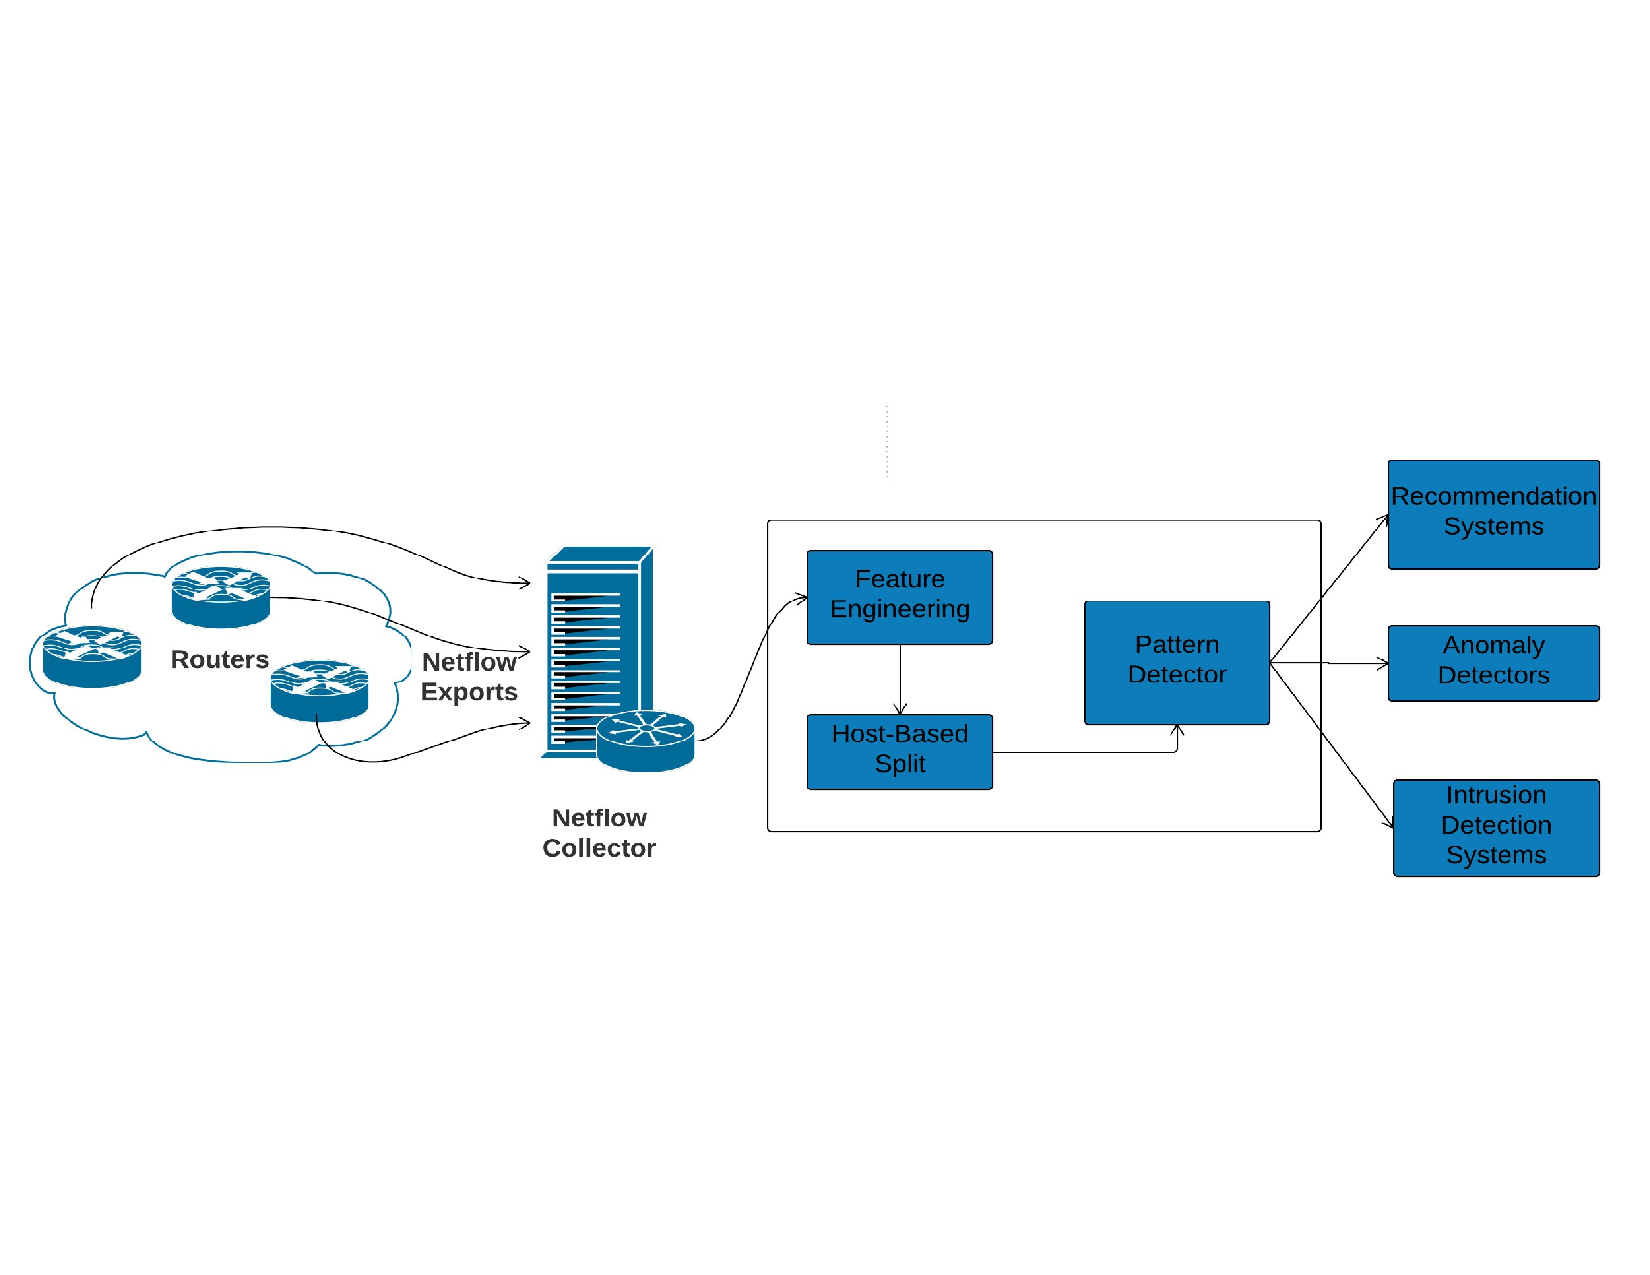
\includegraphics[trim=4cm 4cm 4cm 4cm, scale = 0.6]{architecture.pdf}}
	\caption{Architecture.}%
	\figlabel{arch}
\end{figure}

\subsection{NetFlow collection}
While the term NetFlow has become a de-facto industry standard, many other network hardware manufacturers support alternative flow technologies namely Jflow, s-flow, NetStream, etc.. The University routers from which we have collected the data for this experiment have been equipped with NetFlow on it which led to using NetFlow as our flow technology. 
\subsubsection{What is NetFlow?}
NetFlow is a proprietary protocol for collecting IP flow packets information on networks. There are different variants to this protocol but across all these versions a flow is defined uniquely by its source and destination IP addresses, source and destination ports, transportation protocol. Whenever one of these values changes a new flow is created. For each flow the number of packets, bytes and other network related information are tallied and stored in the routers cache till it expires, then this information is exported to a collector. 

The captured flows are exported to NetFlow collectors at frequent intervals. The flows that are to be exported are determined based on the following rules: 1) When a flow is inactive for a certain time without receiving any new packets. 2) If the flow is active than max threshold time which is configurable. 3) If a TCP flag (FIN / RST) indicates the flow is terminated. NetFlow provides a powerful tool to keep track of what kind of traffic is going on the network, and are widely used for network monitoring. Most vendors support different flavors of similar flow monitoring approaches and a common standardization is done within the IETF IPFIX working group.

There are different variants of NetFlow with each advanced version giving additional information about the flow. The fields that we used in our experiment and that are supported across the versions are in \figref{netflow}.

\begin{figure}[t]
	\centerline{
	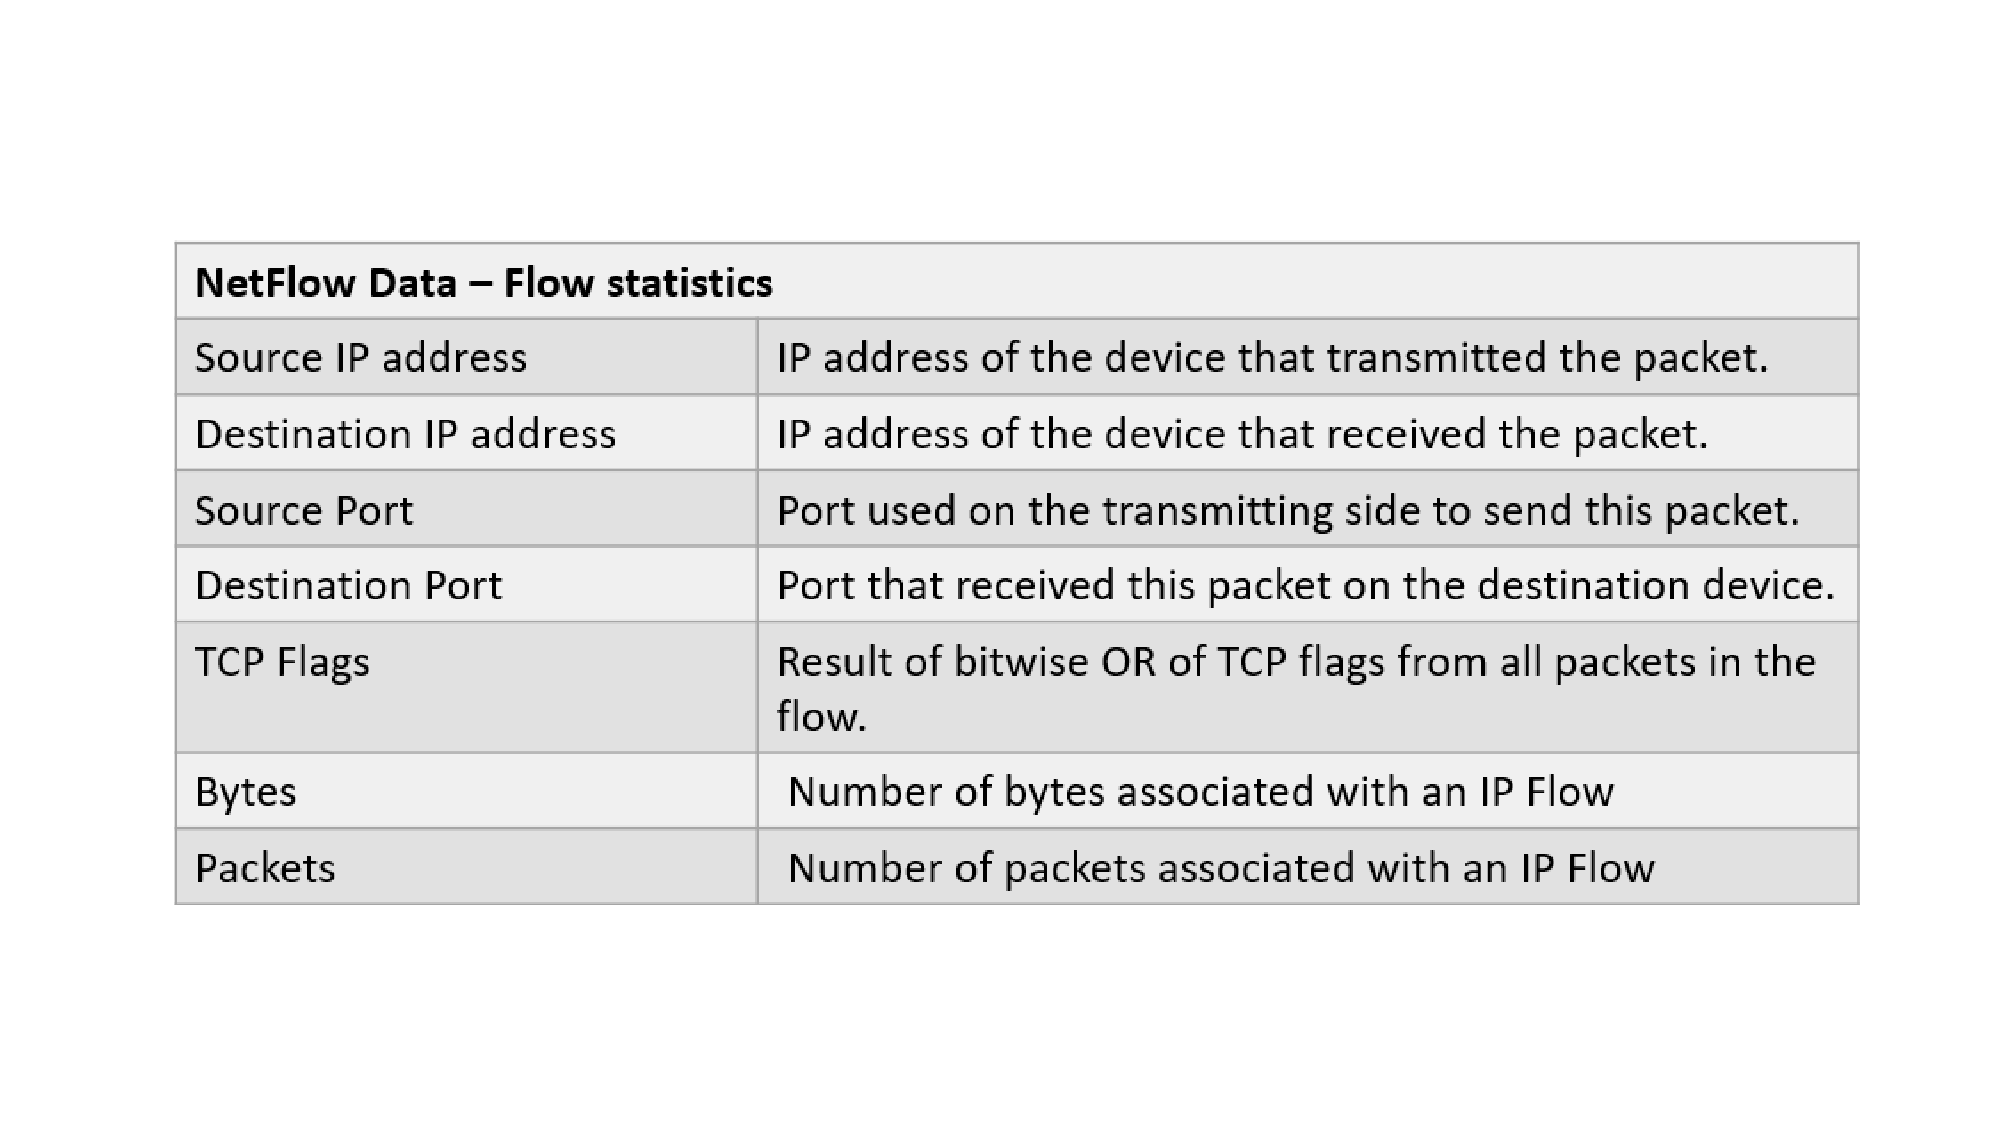
\includegraphics[trim=2cm 2cm 2cm 2cm, scale = 0.55]{netflow.pdf}}
	\caption{NetFlow Fields captured in a Flow }
	\figlabel{netflow}
\end{figure}

\subsection{Feature Engineering}

Feature Engineering is the process of transforming raw
data into features so as to better represent the underlying structure of the data. This helps in increasing the accuracy of the models we build using data mining techniques. This step comes before modeling and after seeing the data.
Features extracted from the data directly influence the models generated and predictions made out of it. The better the features are the better the results will be. The results that we achieve when we are using DM approaches are a factor of the data set in hand, the features generated , the prediction model and the way the problem is framed. Most of the times even simpler models perform better if the features describe the structure inherent to the data. 
Below we describe different steps involved in the Feature Engineering with sample set of data.
\begin{table}[t]
	\caption{Netflow raw data.}%
	\centerline{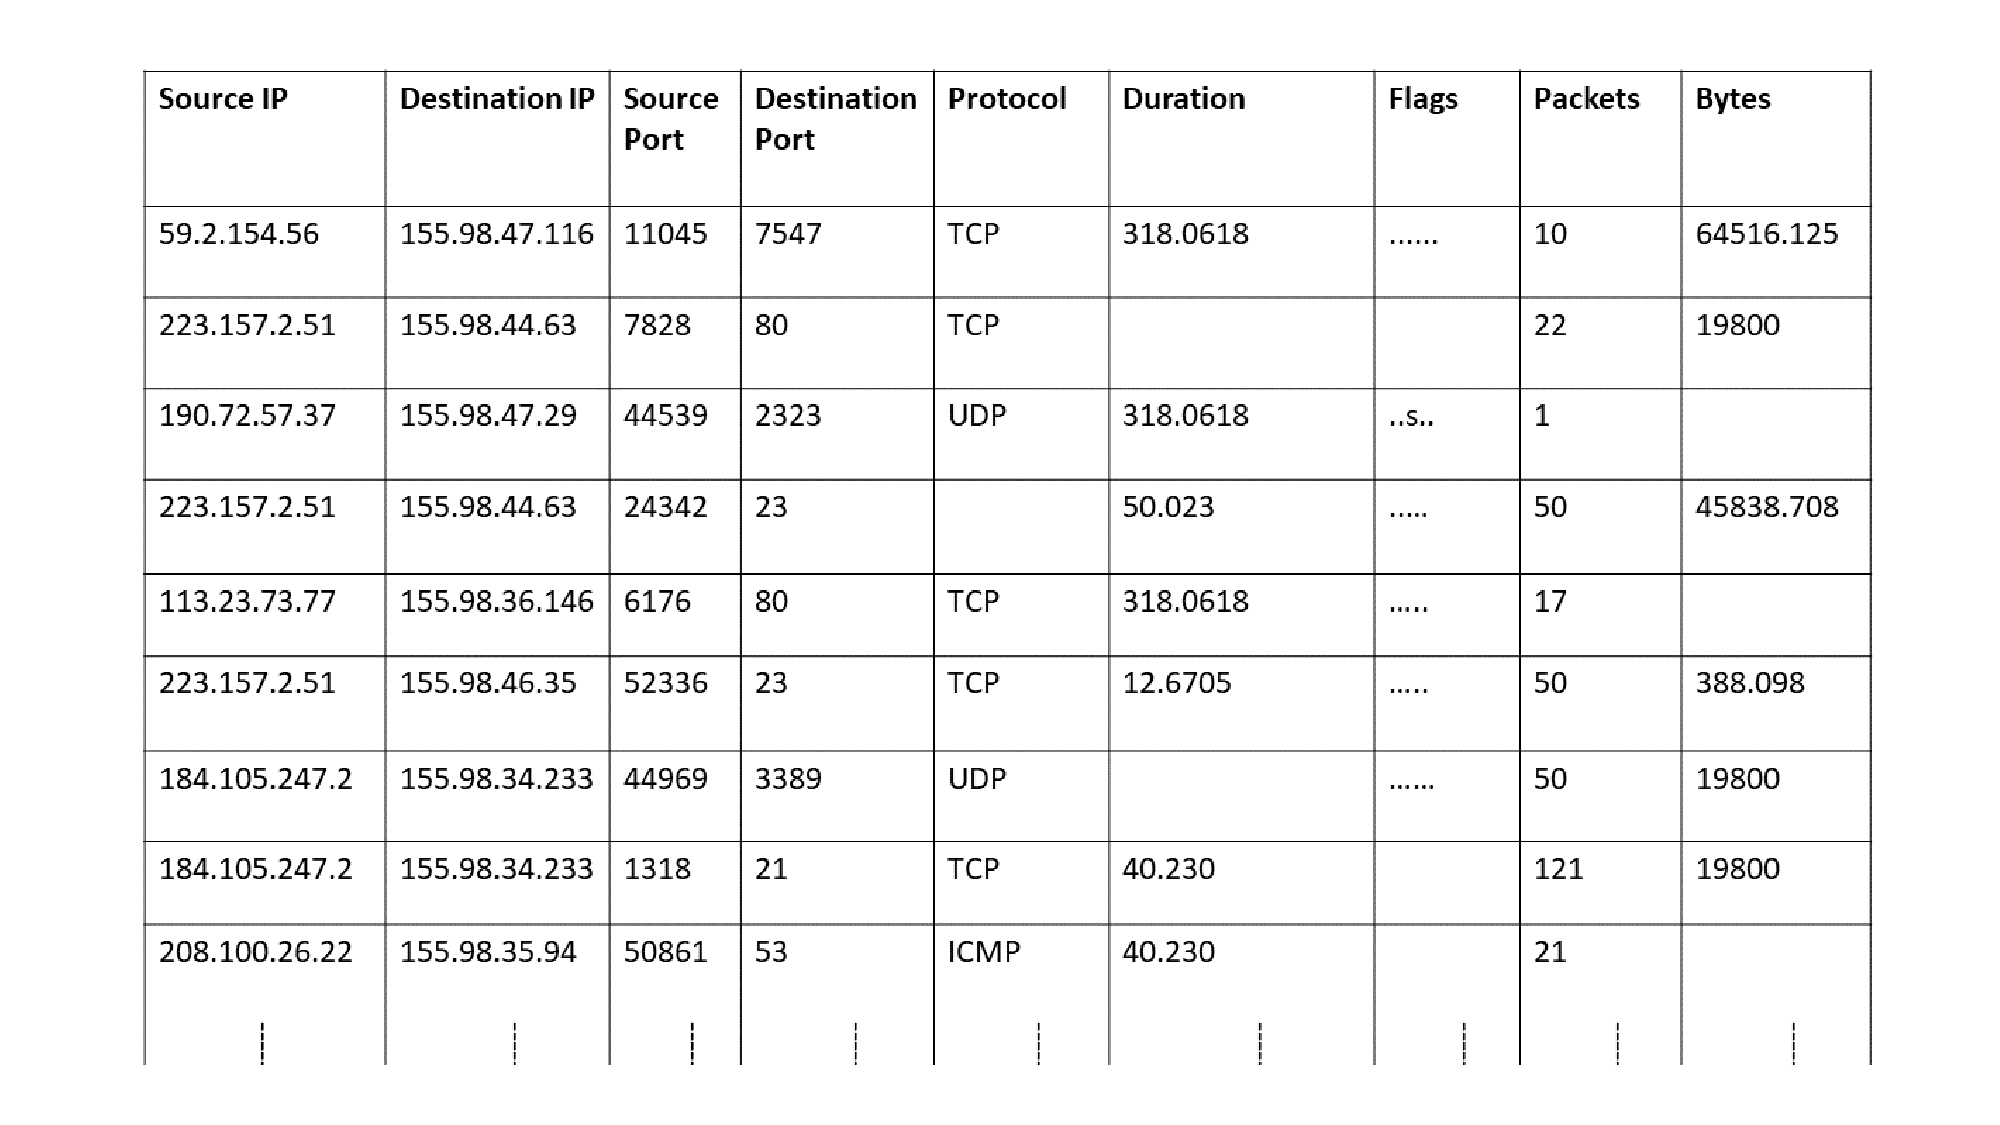
\includegraphics[scale = 0.5]{raw_data.pdf}}	
	 \tablabel{raw_data}
\end{table}
 
\subsubsection{Missing Data} 

\tabref{raw_data} is a sample of network data collected using NetFlow. In total there are 40 columns (only 9 columns are shown in the table) for each record with each column capturing different flow information. From the table we can see that there are few missing values. Missing data is a common issue that every data science experiment has to deal with and there could be different reasons why NetFlow records could be missing some values such as, few filters could be turned on the router that doesn't let the NetFlow collector collect all the information, overloading of NetFlow collector and others. We handled Missing data using the following techniques 

1) Replace missing values with the mean. For the features such as duration, total packets and bytes exchanged we assume that missing values are distributed similarly to the values that are present for each source IP. The rational approach here would be to substitute values using mean as it maintains the existing distribution.

2) Replace missing values with the median/ mode. This is an other technique to handle missing data, It should be noted that using different statistical measures to replace missing values yield different solutions. Features that have categorical data cannot be handled using mean or median and hence we approach mode to fill in their missing values. The feature protocols was handled using the mode approach, filling the missing values with the most frequently occurring protocol value for that source IP.

3) The question that arises when replacing missing values is what percentage of values can a feature miss atmost. For example, filling in half the values of a feature in this step with a statistic measure is not reasonable. Features of this kind are considered as noise and could affect the effectiveness of the data mining algorithm. The better option here would be to discard the coulmn that has too may missing calues. In our case there were handful of columns that fell under this category and are discarded. flags shown in the \tabref{raw_data} is one among them. After handling missing values our data looks as in \tabref{missing_data}.

\begin{table}[t]
	\caption{NetFlow raw data after handling missing values}%
	\centerline{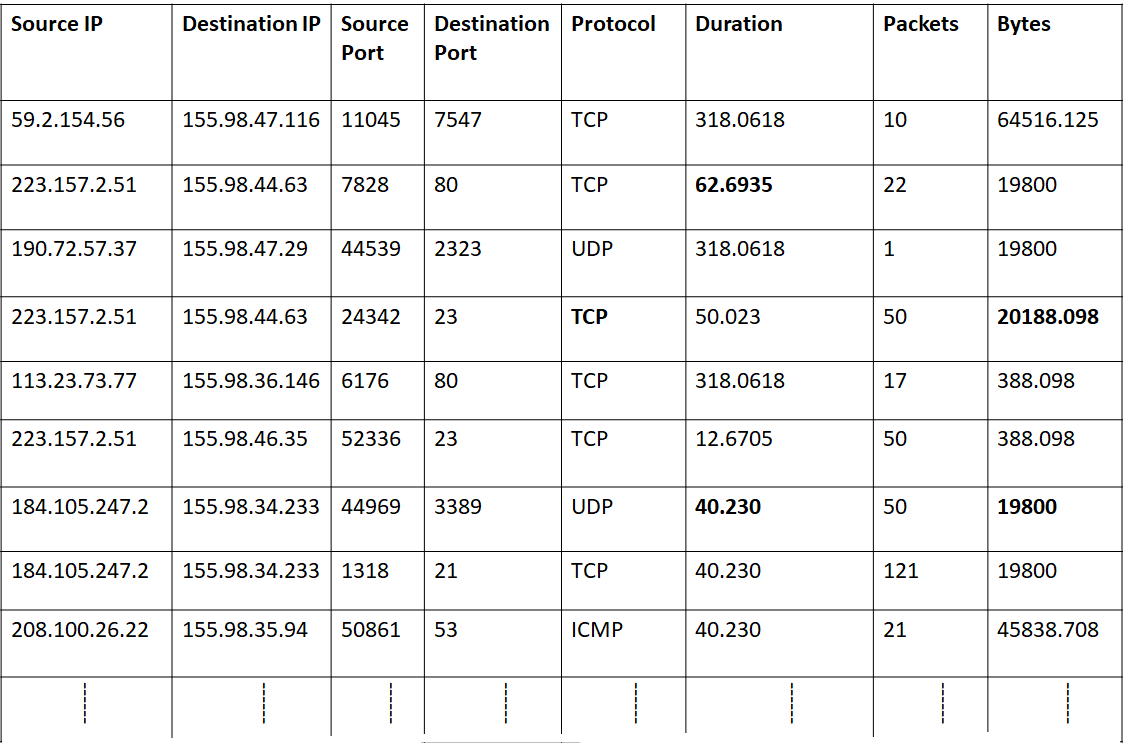
\includegraphics[scale = 0.6]{missing_data.png}}
	
	\tablabel{missing_data}
\end{table}


\subsubsection{Converting Categorical to Numerical Variables} 

Features could be either numerical or categorical variables. When dealing with algorithms that work on numerical data we have to make sure that the categorical variables are handled.
For example, in our case feature protocol, has values such as TCP, UDP and others. One approach is to encode them as 0, 1, and 2 respectively converting them to numerical variables. This could pose a problem when using distance measuring algorithms as the distance between the encoded attributes, like 1 (UDP) ,0 (TCP) is smaller than 0 (TCP) ,2 (others) generating an unintended meaning to this feature and could lead to biasing of few values. Another approach would be to create a feature for each value of the categorical variable and mark it as 0 or 1 based on if the value is present or not. There are both pros and cons to this method. The pros are if we choose to aggregate the values on all features this conversion gives a numerical value to work with. The cons are scaling and standardization could be affected. \tabref{categorical} represents data set after this step.

\begin{table}[t]
	\caption{After Converting categorical data to numerical}%
	\centerline{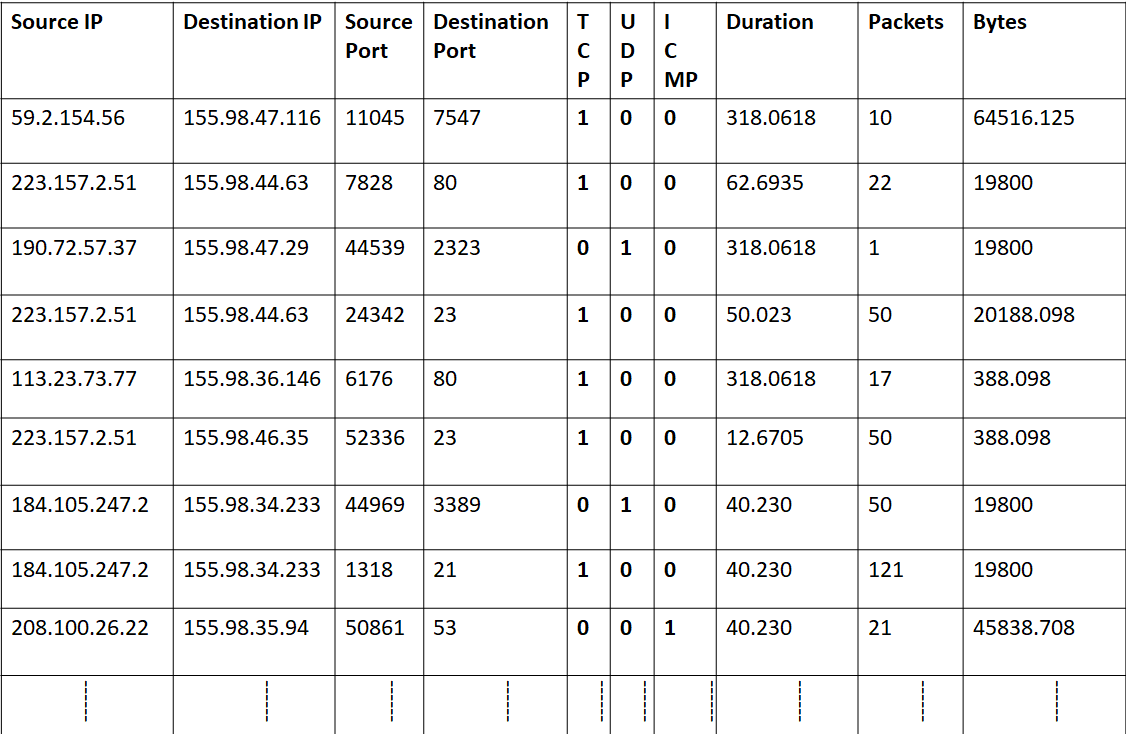
\includegraphics[scale = 0.6]{categorical.png}}
	\tablabel{categorical}
\end{table}

Above two steps fall under a family of techniques called data cleaning. After the data cleaning and removing the irrelevant columns of data using domain knowledge we aggregated NetFlow data based on source IP as our work focuses learning about hosts from their aggregate data. The \tabref{aggregated} shows a sample of aggregated data with ten features.
The first record in the \tabref{aggregated} conveys the information that in the given data set the host 59.2.154.56 (source IP) had appeared 450 times. Out of those 450 instances it had contacted 116 unique hosts. A total of 110 different source ports were used in the 450 flows and all the packets were sent to single destination port. The columns TCP, UDP, ICMP indicate how many of these flows fall under each category. So of the 450 flows there are 406 flows in which TCP protocol was used , 4 had UDP protocol used and the rest 40 had used ICMP protocol. And the columns Total Duration, Total Bytes, Total Packets indicate the respective information exchanged by this sourceIP on a whole. This aggregated data is what we use for learning host behaviors. But, before that we have to apply few other feature engineering techniques as described below.

\begin{table}[b]
	\caption{Aggregated data by Source IP}%
	\centerline{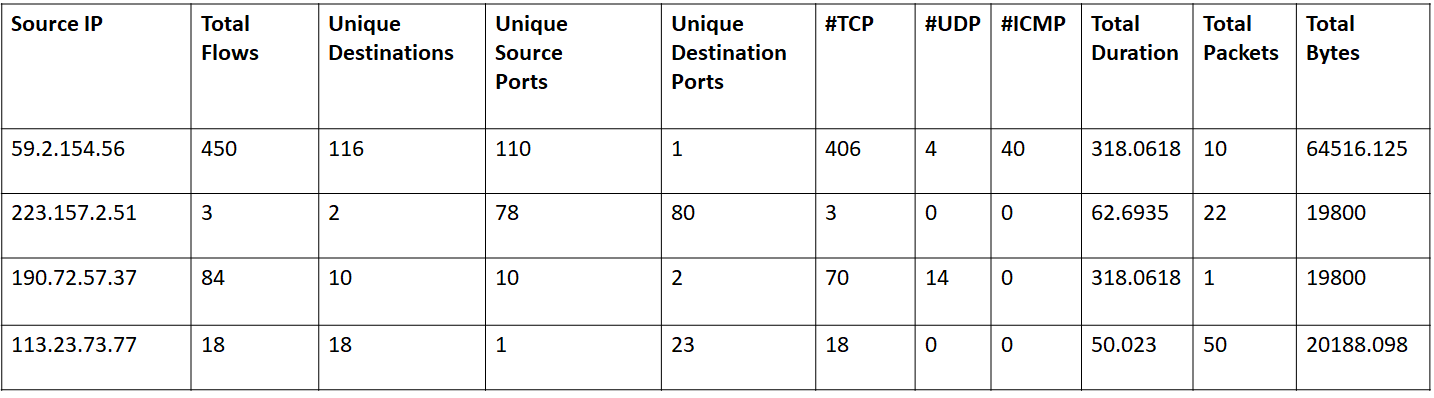
\includegraphics[scale = 0.6]{aggregated.png}}	
	\tablabel{aggregated}
\end{table}


\subsubsection{Feature Scaling} 
Feature Scaling/Feature Normalization, a method used to standardize the range of independent features of data. Failure to standardize variables might result in algorithms placing undue significance to variables that are on a higher scale. For example from the \tabref{aggregated} it is evident that the total packets and total bytes have higher magnitude compared to total flows and destinations. This range difference shouldn't bias our results.
There are different ways to do feature scaling namely, Min-Max scaling, Variance scaling, L2 normalization etc.. The choice depends on the data and different statistics of it such as Mean, Variance, L2 norm. Scaling is not advisable in all instances we might	loose valuable information if applied without proper thought. In our case we have chosen simple Min-Max scaling as our goal was merely to change the range of the data and not the distribution and Min-Max scaling helps us in achieving this at a lower cost.

\subsubsection{Feature Transformation} 
Transforming Non-normal distribution to Normal, many ML/DM tools perform well on normalized data and having skewed data will give inaccurate results. Log transformations are generally used to normalize the skewed data which is the case with most network data. After transforming the data if it doesn't capture the essence of original data we could look at other options such as square root, cube root. BoxCox is also another technique that changes the distribution of variables from non-normal to normal or near normal. \figref{feature} shows the distribution of a feature Total Flows from our aggregated data, as seen from the graph it is heavily skewed towards left and this can be directly attributed to the data set we have in hand. The graph indicates that in most instances number of flows in which a source IP appears is less than 100 and hence we employ transformation techniques to decrease the amount of skewness in the data.  \figref{feature_transformed} shows the same data after applying log transformation. 

\begin{figure}[t]
	\centerline{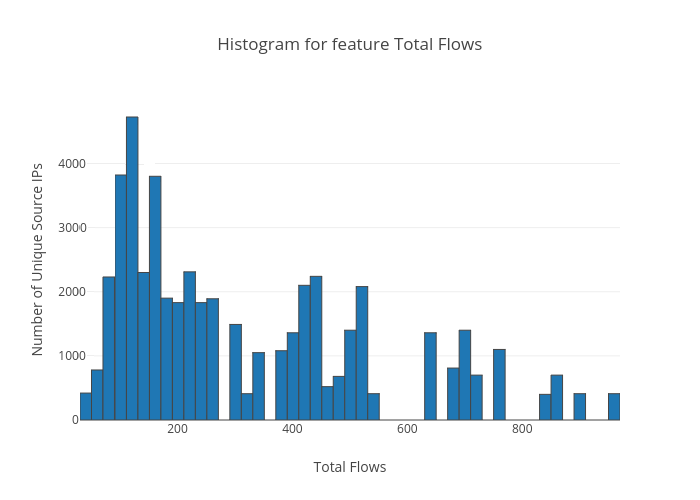
\includegraphics[scale = 0.9]{feature.png}}
	\caption{Skewed data before transformation}%
	\figlabel{feature}
\end{figure}

\begin{figure}[t]
	\centerline{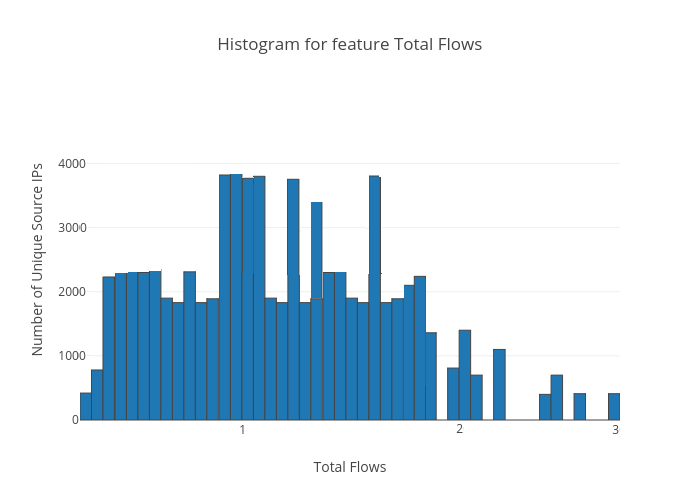
\includegraphics[scale = 0.9]{transformed.png}}
	\caption{Normalized data}%
	\figlabel{feature_transformed}
\end{figure}



\subsubsection{Feature Selection}		
	
	Feature Selection refers to the process of selecting a subset of relevant features to model the data. It helps in shorter time periods of execution, overcoming the overfitting problem and making the solution more generic and avoid curse of dimensionality. The central premise of this process is to remove redundant or irrelevant features that don't make much sense to the problem we ought to solve. Feature selection and dimensionality reduction are two confusing terms. Though, both methods seek to reduce the number of attributes in the dataset, but dimensionality reduction does it by creating new combinations of attributes, where as feature selection methods include and exclude attributes present in the data without changing them. Principal Component Analysis, Singular Value Decomposition are examples of dimensionality reduction methods. The techniques used to do feature selection depend on text, numerical variables and they are three general classes of them Filter, Wrapper, Embedded methods.	Feature selection is a much tougher problem in unsupervised setting as we don't have any labels that helpus in determining the information gain with and without a feature.Problems of
	this kind have been rarely studied in the literature \cite{boutsidis2009unsupervised} \cite{dash2002feature}. 
	
	The common strategy of most approaches is the use of filter methods Filter model methods do not utilize any clustering algorithm to test the quality of the features. They evaluate the score of each feature according to criteria \cite{dash2002feature} mentioned here. It selects the features with the highest score. It is called the filter since it filters out the irrelevant features using given criteria. 
	Wrapper methods are an other class of methods used for feature selection where we train the given model with different combinations of features and make inferences accordingly.
	Some common examples of wrapper methods are forward feature selection, backward feature elimination and recursive feature elimination. Forward selection is similar to elbow method explained in the next section. It is an iterative technique where we start with zero features and in each step we keep adding feature that has the most information gain or best expresses the underlying structure. This procedure is stopped when addition of an extra feature doesn't add any significant information to the model. forward The backward eliminaion technique is exactly opposite to the Forward selection method. Here we start with all the features and remove the least significant feature at each iteration. This iterative procedure stops when no improvement is observed on removal of features.
	
	We have chosen wrapper methods backward elimination technique for feature selection as it measures the usefulness of a subset of features by actually training a model on it. Though, it is computationally expensive compared to Filter based approaches in our context it was reasonable as we had only 10 features to look into. The result of feature selection is we have detected two features that have very less information gain namely the ICMP ports and duration and hence we removed these two from our feature list making our final feature count to 8.
	 Feature Selection has helped us in enabling the machine learning algorithm to train faster. It reduced the complexity of the model and made it easier to interpret. We were also able to address the overfitting problem.






\section{Pattern Detector}
Pattern Detector consists of the core logic of our system. After cleaning the data and applying feature engineering we send the data through a pattern detector. Pattern Detector sends the data through a clustering algorithm. It then maps the generated clusters to the host behaviors which is explained later.

As mentioned in the background section we choose to address our problem using unsupervised learning approaches. The most common unsupervised learning method is cluster analysis, which is used for exploratory data analysis to find hidden patterns or grouping in data. 

\subsubsection{Why K-Means ??}
 In the section \ref{unsupervised} we have discussed about different type of clustering techniques in detail. Here we provide a reasoning for choosing K-Means.
 
Connectivity models like Hierarchical clustering don't have a provision for relocating objects that may have been incorrectly grouped at an early stage. Also, use of different distance metrics for measuring distances between clusters may generate different results. Performing multiple experiments and comparing
the results is recommended to support the veracity of
the original results. Lastly, time complexity of at least O($n^2logn$) is required, where n is the number of data points thus lacking scalability for handling big datasets.

Distribution Models assume a distribution for data but for many real data sets, there may be no concisely defined mathematical model (e.g. assuming Gaussian distributions is a rather strong assumption on the data). Also, though distribution models have an excellent  theoretical foundation but they suffer from one key problem known as overfitting. 

We have experimented our data set with the density model DBSCAN and we have found the data being grouped at most in to only two clusters. The reason for this is that density based models expect some kind of density drop to detect cluster borders. Recall from the above section that our data set has many source IPs that appear in less than 100 flows and hence there wasn't any drop in density observed resulting in bad clustering.

Experimenting with centroid models especially K-Means gave us an advantage to play with the variable K and view into how host behaviors are being grouped with different values of K. It is scalable for heavier datasets and doesn't suffer from the overfitting problem. Also, there isn't any inherent assumption on which distribution the dataset should follow. Thus, making it a clear choice for building our system.


\subsubsection{How to choose K ??}
 In many situations, parameters and variables chosen by the algorithm or by users affects the performance of the algorithm differently and results in different outputs. Similarly, an essential problem of the K-means clustering method is to define an appropriate number of clusters K. In the literature there are different approaches proposed to determine an accurate value of K.
 These methods include direct methods and statistical testing methods. Direct methods consists of optimizing a criterion, such as the within cluster sums of squares or the average silhouette. The corresponding methods are named elbow and silhouette methods, respectively. Statistical testing methods consists of comparing evidence against null hypothesis. An example is the gap statistic. We have used the direct methods as they optimize a criteria the elbow method to determine K and then cross-verified the values with the Silhouette Index obtained for this same data set.
 
 Recall that, the basic idea behind partitioning methods, such as k-means clustering, is to define clusters such that the total intra-cluster variation [or total within-cluster sum of square (WSS)] is minimized. The total WSS measures the compactness of the clustering and we want it to be as small as possible. The Elbow method looks at the total WSS as a function of the number of clusters: One should choose a number of clusters so that adding another cluster doesn’t improve much better the total WSS. 
 The optimal number of clusters can be defined as follow:
 \begin{itemize}
 	\item Compute k-means clustering for different values of k. For instance, by varying k from 1 to 50 clusters.
 	
 	\item For each k, calculate the total within-cluster sum of square ($W_k$).
 	\begin{center}
 	 	\boldsymbol{$D_k = \sum_{x_i \in C_k} \sum_{x_j \in C_k} ||{x_i -x_j}||^2$}	 \\
 	 	
 	 	
 	 	\boldsymbol{$ W_k = \sum_{1}^{K} \frac{1}{n_k} D_k$}
 	\end{center}  
    Where K is the number of clusters, $n_k$ is the number of points in cluster k and $D_k$ is the sum of distances between all points in the cluster.
 	\item Plot the curve of wss according to the number of clusters k. 	
 	\item The location of a bend (knee) in the plot is generally considered as an indicator of the appropriate number of clusters.
 \end{itemize}

 	The graph depicts the amount of information we are gaining with addition of each cluster. the first clusters will add much information, but at some point the marginal gain will drop, giving an angle in the graph. The number of clusters are chosen at this point, hence the elbow criterion. \figref{elbow} shows the elbow curve obtained for our data set on a chosen day. This method gave us a value of 7 for K.
 	

\begin{figure}[t]
	\centerline{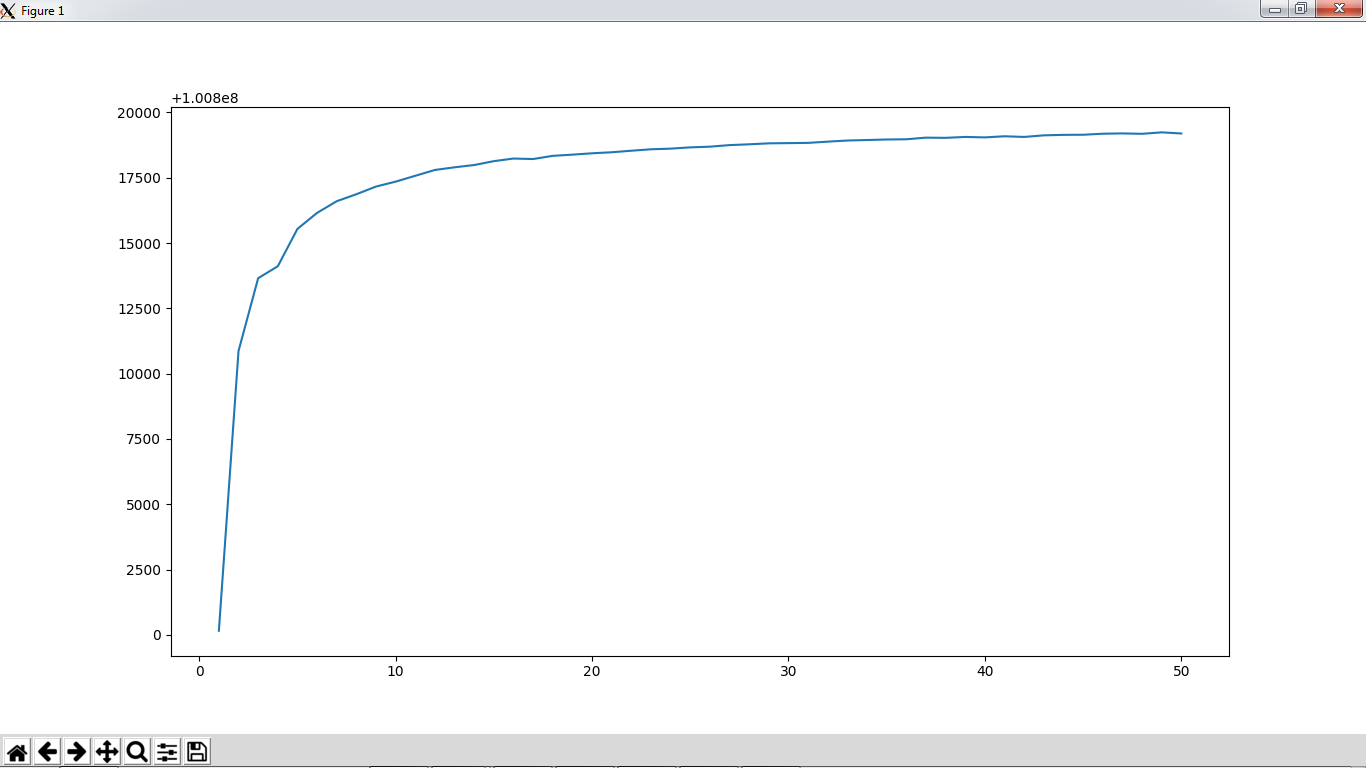
\includegraphics[scale = 0.4]{elbow.png}}
	\caption{Elbow Method}%
	\figlabel{elbow}
\end{figure}

 However, the elbow method is not unambiguous. especially if the data is not very clustered we will notice that the elbow chart will not have a clear elbow. Instead, we see a fairly smooth curve, and it's unclear what is the best value of k to choose. In cases like this, we might try a different method for determining the optimal k. Hence, to corroborate the claim of elbow method for K we also ran our data set through another technique called silhouette.

	The average silhouette approach measures the quality of a clustering. That is, it determines how well each object lies within its cluster. A high average silhouette width indicates a good clustering.	Average silhouette method computes the average silhouette of observations for different values of k. The optimal number of clusters k is the one that maximize the average silhouette over a range of possible values for k.	The algorithm is similar to the elbow method and can be computed as follow: 
	
	\begin{itemize}
		\item Compute k-means clustering for different values of k. For instance, by varying k from 1 to 50 clusters.
		\item For each k, calculate the average silhouette of observations (avg.sil).
		
		\begin{center}
			\boldsymbol{$s(i) = \frac{b(i) - a(i)}{max(a(i),b(i))}$}
		\end{center}
		Here s(i) is the silhouette index of a cluster point i. Where a(i) is the average distance of point i to all the objects in the same cluster while b(i) is the minimum average distance from the point i to all the points of different cluster. avg.sil is calculated by finding mean of all the s(i) for each point in a cluster.
		
		\item Plot the curve of avg.sil according to the number of clusters k.
		\item The location of the maximum is considered as the appropriate number of clusters.
	\end{itemize}
 
  The intuition behind this approach is for a point as a(i) is a measure of how dissimilar i is to its own cluster, a small value means it is well matched. Furthermore, a large b(i) implies that i is badly matched to its neighboring cluster. Thus an s(i) close to one means that the data is appropriately clustered. if s(i) is close to negative one, then by the same logic we see that i would be more appropriate if it was clustered in its neighboring cluster. The average s(i) over all data of a cluster is a measure of how tightly grouped all the data in the cluster are. Thus the average s(i) over all data of the entire dataset is a measure of how appropriately the data have been clustered. \figref{silhouette} shows the the plot obtained using silhouette technique. 
 
   An important point that has to be noted here is that, though we have a method to evaluate K, we don't invoke this method daily to determine the K value. We chose a reference day and determine the K value for that day and that K value is used for the remaining days till the network admin chooses to change this reference day. A reference day is selected generally to reflect all the behaviors that are seen in our network in day-to-day basis. The choice of changing this reference day also vests with the network admin as he knows how the usage of network has been changed and whenever a reference day is changed we need to calcualte the K value again.
   
 \begin{figure}[t]
 	\centerline{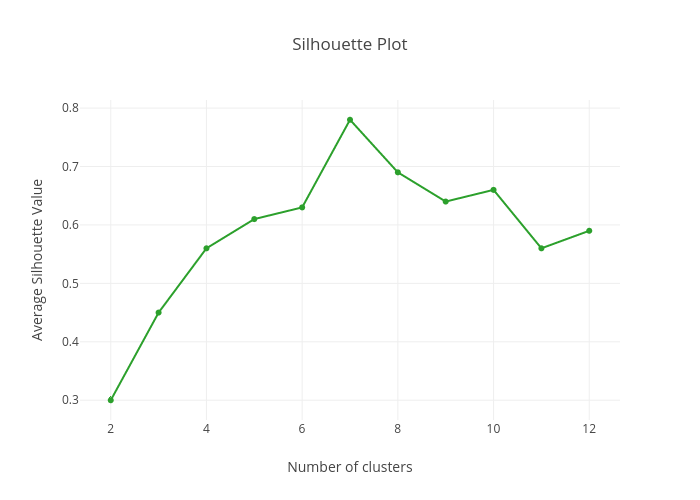
\includegraphics[scale = 0.6]{silhouette.png}}
 	\caption{Silhouette Method}%
 	\figlabel{silhouette}
 \end{figure}
 
\subsubsection{Cluster Labeling and Comparison}  \label{cluster_labeling}

The output of the pattern detection step is a set of clusters. We explored these clusters to better understand the grouping of hosts. We observed that each cluster exhibits a unique behavior. That is all the hosts in a cluster exhibit similar behavior. These clusters were labeled accordingly.
Recall the overarching premise of our work is to analyze the behavior of hosts looking at the aggregated host data. In order to analyze the behavior of hosts over a time period we should be able to compare hosts behavior across days. We dealt with this by initially comparing the hosts behavior for any two days and then extended it to any given time period. To achieve this we chose a reference day and label the clusters on that day through manual inspection. On any other day we label the clusters by comparing it with this reference day. Cluster comparison is an active research area but in our case it is slightly easier to solve because the number of clusters that are formed on each day are constant (i.e, as we choose the same k value as on reference day.) and each cluster maps to a unique behavior. So, all that we need to do is to find a one-to-one mapping with the reference day clusters. 
Now this turns out to be an assignment problem which is well studied \cite{kuhn1955hungarian}. Assignment problem is a special type of linear programming problem which deals with the allocation of the various resources to the various activities on one to one basis. It does it in such a way that the cost or time involved in the process is minimum and profit or sale is maximum. 

In our case both the resources and activities are nothing but clusters formed on two different days and this has to be done in such a way that the total effort is least. Assignment Problem is a well studied problem and has polynomial time solutions. One such algorithm is the Hungarian algorithm\cite{}.

\section{Applications} \label{applications}
Our system can be used to build different applciations that help in network management as listed below.
\begin{itemize}
	
	\item \textit{Anomaly Detectors}, applications that expose the hosts that are behaving as outliers and don't conform to an expected pattern. We can use our system to build such applications. For example, we found a cluster of hosts that are exhibiting anamolous behavior during our exploration of  emulab data. We can observe the change of this cluster size and center over days and there by notify the network admin if there is a shift in anamoly behavior that network admin has to be aware of. Here we can take the help of  work done by \cite{} to determine when should a network admin be notified. 
	
	\item \textit{Dynamic Security Rules Generator}, Looking at the historic user behavior we can generate dynamic rules for security of the network. Few of them could be, to block certain ips that are exhibiting inconsistent behavior etc. Authentication rules can also adapt dynamically by observing the changes of different clusters and their cluster centers. Such as, number of unsuccessful attempts a client can make to a server can also be limited based on the different ports client is using.
	
	\item \textit{Recommendation Systems}, We can capture the different behaviors exhibited by network users over time and use this to predict a behavior on a certain day of a week or month using the historical data. This helps network admin to prepare well ahead and plan the bandwidth or other network resources accordingly.
	
	In this direction of building applications through the results obtained from our system we have created a web tool that analyzes data in different dimensions and is explained in detail in evaluation chapter.

\end{itemize}


 

%In that direction of building a recommendation system we came up with an user interface that helps to analyze historic data , this should go into evaluation section.%





% \numberofappendices = 1   % Set 0 for none, else number of appendices.
\numberofappendices = 0
%\appendix       % Chapters, sections are now appendix style A, A.1, A.2, B, C, D, ...

%%%% -*-LaTeX-*-

\chapter{The First}

This is an appendix.  Notice that the \LaTeX{} markup for an appendix
is, surprisingly, \verb=\chapter=.  The \verb=\appendix= command does
not produce a heading; instead, it just changes the numbering style
from numeric to alphabetic, and it changes the heading prefix from
\textbf{CHAPTER} to \textbf{APPENDIX}.

\blah \blah \blah

%%%% -*-LaTeX-*-

\chapter{The Second}

This is an appendix.

\blah \blah \blah

\index{gnu hair}
\index{gnu  hair}
\index{ gnu  hair}
\index{ gnu hair }
\index{E. coli bacterium@\bioname{E. coli} bacterium}

\index{GNU Project}
\index{gnu}

\index{gnu!diet}
\index{gnu!diet!wet season}
\index{gnu!diet!dry season}

\index{gnu!predators}
\index{gnu!predators!crocodiles}
\index{gnu!predators!hyenas}
\index{gnu!predators!lions}

\index{Connochaetes gnou@\bioname{Connochaetes gnou}}

%%%% -*-LaTeX-*-

\chapter{The Third}

This is an appendix.

There are several books
\cite{%
    Singh:1997:FEE,%
    Salomon:1995:AT,%
    Robbins:2005:CSS,%
    Randell:1982:ODC,%
    Olver:2010:NHM,%
    Mittelbach:2004:LC,%
    Lamport:1985:LDP,%
    Knuth:1999:DT,%
    Knuth:1986:TB,%
    Knuth:1986:MB,%
    Farmelo:2009:SMH%
}
listed in our bibliography.

We also reference several journal articles
\cite{%
    Wiles:1995:MEC,%
    Taylor:1995:RTP,%
    Lahiri:2002:ADA,%
    Kim:1999:AFC,%
    Johnson:1978:LDT,%
    Huskey:1980:LLC,%
    Heilbron:1969:GBA,%
    Hall:1994:PNE,%
    Goldstine:1946:ENI,%
    Einstein:1911:BMAb,%
    Einstein:1911:BMAa,%
    Einstein:1906:NBM,%
    Cody:1981:APF,%
    Beebe:1989:PCP,%
    Babbage:1910:BBA%
}
and three famous doctoral theses of later winners
\cite{%
    Einstein:1905:NBM,%
    Dirac:1926:QM,%
    Bohr:1911:SME%
}
of the Nobel Prize in Physics (1922, 1933, and
1921):

Notice that, even though those citations appeared
in \LaTeX{} \verb=\cite{...}= commands with their
\BibTeX{} citation labels in reverse alphabetical
order, thanks to the \verb=citesort= package,
their reference-list numbers have been sorted in
numerically ascending order, and then
range-reduced.

Mention should also be made of a famous Dutch
computer scientist's first publication
\cite{Dijkstra:1953:FBV}.

Font metrics are an important, albeit low-level,
aspect of typesetting. See the \emph{Adobe
Systems} manual about that company's procedures
\cite{Adobe:1990:AFM}.

The bibliography at the end of this thesis contains several examples
of documents with non-English titles, and their \BibTeX{} entries
provide title translations following the practice recommended by the
American Mathematical Society and SIAM\@.  Here is a sample entry that
shows how to do so:
%
\begin{verbatim}
@PhdThesis{Einstein:1905:NBM,
  author =       "Albert Einstein",
  title =        "{Eine Neue Bestimmung der Molek{\"u}ldimensionen}.
                 ({German}) [{A} new determination of molecular
                 dimensions]",
  type =         "Inaugural dissertation",
  school =       "Bern Wyss.",
  address =      "Bern, Switzerland",
  year =         "1905",
  bibdate =      "Fri Dec 17 10:46:57 2004",
  bibsource =    "http://www.math.utah.edu/pub/tex/bib/einstein.bib",
  note =         "Published in \cite{Einstein:1906:NBM}.",
  acknowledgement = ack-nhfb,
  language =     "German",
  advisor =      "Alfred Kleiner (24 April 1849--3 July 1916)",
  URL =          "http://en.wikipedia.org/wiki/Alfred_Kleiner",
  remark =       "Received August 19, 1905 and published February 8,
                 1906.",
  Schilpp-number = "6",
}
\end{verbatim}

The \texttt{note} field in that entry refers to another bibliography
entry that need not have been directly cited in the document text.
Such cross-references are common in \BibTeX{} files, especially for
journal articles where there may be later comments and corrigenda that
should be mentioned.  Embedded \verb=\cite{}= commands ensure that
those possibly-important other entries are always included in the
reference list when the entry is cited.  The last bibliography entry
\cite{Wiles:1995:MEC} in this thesis has a long \texttt{note} field
that tells more about what some may view as the most important paper
in mathematics in the last century.

When entries cite other entries that cite other entries that cite
other entries that \ldots{}, multiple passes of \LaTeX{} and \BibTeX{}
are needed to ensure consistency.  That is another reason why document
compilation should be guided by a \texttt{Makefile} or a batch script,
rather than expecting the user to remember just how many passes are
needed.

\BibTeX{} entries are \emph{extensible}, in that arbitrary key\slash
value pairs may be present that are not necessarily recognized by any
bibliography style files.  The \texttt{advisor},
\texttt{acknowledgement}, \texttt{bibdate}, \texttt{bibsource},
\texttt{language}, \texttt{remark}, and \texttt{Schilpp-number} fields
are examples, and may be used by other software that processes
\BibTeX{} entries, or by humans who read the entries.  \texttt{DOI}
and \texttt{URL} fields are currently recognized by only a few styles,
but that situation will likely change as publishers demand that such
important information be included in reference lists.

In \BibTeX{} \texttt{title} fields, braces protect words, such as
proper nouns and acronyms, that cannot be downcased if the selected
bibliography style would otherwise do so.  In German, all nouns are
capitalized, and the simple way to ensure their protection is to brace
the entire German text in the title, as we did in the entry above.

The world's first significant computer program may
have been that written in 1842 by Lady Augusta Ada
Lovelace (1815--1852) for the computation of Bernoulli
numbers \cite{Huskey:1980:LLC,Kim:1999:AFC}.  She
was the assistant to Charles Babbage
(1791--1871), and they are the world's first
computer programmers. The programming language
\emph{Ada} is named after her, and is defined in
the ANSI/MIL-STD-1815A Standard; its number
commemorates the year of her birth.

We do not discuss mathematical \emph{transforms}
in this dissertation, but you can find that phrase
in the index (except that this sample thesis doesn't have one!)

\blah

\blah
\blah

\blah


%%% The choice of bibliography style is a major decision, jointly made
%%% by you, your thesis advisor and the thesis editor. Common choices are
%%% one of the four standard BibTeX styles (abbrv, alpha, plain, and unsrt),
%%% or enhanced styles like acm, amsplain, siam, and hundreds of others
%%% available in TeX Live, and other Unix and Windows TeX distributions.
%%%
%%% Do NOT handcode your reference list, because you are unlikely to
%%% achieve consistency or conformance to the University of Utah Thesis Office
%%% requirements: let BibTeX do that tedious job for you!
%%%
%%% Remember that reference-list metadata in BibTeX files remains
%%% constant across journals and publishers, and is are often reused
%%% in other documents and shared with others, whereas formatted
%%% reference-list styles change: with BibTeX, you only need to record
%%% the metadata once.
%%%
%%% If you prefer named, rather than numeric or tagged citations, you
%%% may use styles such as authordate{1,2,3,4}, chicago, harvard, or
%%% natbib.  Be aware, however, that most of those require an
%%% additional \usepackage{} command to supply \LaTeX{} with
%%% definitions of commands that the style needs, and that there are
%%% usually several flavors of LaTeX citation commands beyond the
%%% standard \cite{} command that you need to understand before you
%%% can use them properly in your prose.

%%% This tells BibTeX to read siam.bst from the first directory where
%%% it is found in the BSTINPUTS search path:

\bibliographystyle{siam}

%%% This can also specify a comma-separated list (without embedded
%%% spaces) of *.bib files found by BibTeX in its BIBINPUTS search
%%% path.  The argument \jobname means the base name of the top-level
%%% LaTeX file, avoiding an unnecessary filename dependence here.
%%%
%%% BibTeX writes only one .bbl file, no matter how many *.bib files
%%% are listed here, using the name \jobname.bbl.
%%%
%%% LaTeX reads BibTeX's formatted reference list from the file
%%% \jobname.bbl.

\bibliography{\jobname}

%%% The last part of this sample thesis is two specialized indexes,
%%% and a general topic index.  If the companion Makefile is used to
%%% create the DVI or PDF file for this work, the topic index excludes
%%% the lengthy list of free software packages.  However, the biology
%%% names of the first index are included in the topic index.

%%% Switch from thesis double spacing to single spacing for the three
%%% indexes, as a matter of style (to match the reference list), and
%%% for compactness.

\singlespace

%%% Define several index cross references (there are many more such
%%% in chap1.tex, but the examples here give a useful summary of how
%%% they are made):

\index{DCT|see{discrete cosine transform}}
\index{DWT|see{discrete wavelet transform}}
\index{Borel measure ($\mu$)}
\index{mu@$\mu$ (mu)|see{Borel measure}}
\index{Escherichia coli@\bioname{Escherichia coli}|see{E. coli}}
\index{transform|seealso{Discrete DCT Transform}}
\index{transform|seealso{Fast Fourier Transform}}

\renewcommand {\bioname} [1] {\emph{#1}}   % redefine to suppress color and indexing in index
\renewcommand {\fsfname} [1] {\texttt{#1}} % redefine to suppress color and indexing in index

\renewcommand {\indexname} {Binomial Nomenclature Index}

%\input{\jobname-bioname.ind}

\renewcommand {\indexname} {Free Software Index}

%\input{\jobname-fsfname.ind}

\renewcommand {\indexname} {Topic Index}

\overfullrule = 0pt % suppress visible warnings about overfull hboxes
%\printindex

\end {document}
